\documentclass[twoside,a4paper,11pt,openright]{report}

%
% Base packages. Only change if you know what you are doing.
%
\usepackage[utf8]{inputenc}	% input encoding setting
\usepackage[english]{babel}	% english hyphenation
\usepackage{newpxtext}		% font palatino
\usepackage{newpxmath}		% matching math-font
\usepackage[T1]{fontenc}	% font encoding setting
\usepackage{amsmath}		% math extensions
\usepackage{microtype}		% improved microtypography
\usepackage{csquotes}		% contextual quotes
\usepackage{calc}		    % calculation of tex dimensions
\usepackage[%
  inner=25mm,%
  outer=35mm,%
  top=25mm,%
  bottom=30mm,%
  includeheadfoot,%
  headheight=14pt,%
  marginparwidth=25mm%
]{geometry}			        % adjustment of type area
\usepackage{parskip}		% no indentation
\usepackage{emptypage}		% no page numbers on empty pages
\usepackage{array}		    % table extension
\usepackage{graphicx}		% integration of graphics
\usepackage{tikz}
\usetikzlibrary{positioning,calc}
\usepackage{float}		    % adjustment of floating environments
\usepackage{fancyhdr}		% customization of headers and footers
\usepackage{pgfplots}
\pgfplotsset{compat=1.18}

%
% Packages that could be included if needed.
%

%\usepackage{biblatex}		% bibliographie
%\usepackage[style=ieee]{biblatex}
%\addbibresource{citationDB.bib}
%\usepackage{textcomp}
\usepackage{xcolor}		% colours
\usepackage{subcaption}	% subnumbering for illustrations
%\usepackage{subfig}

\usepackage{listings}		% source code listings
\lstset{basicstyle = \ttfamily,columns=fullflexible}
%\usepackage{listingsutf8}
%\usepackage{units}		% physical units
% TODO: caption
\captionsetup{
    labelsep=colon,
    format=hang
}
% TODO: rotating
% TODO: paralist
% TODO: tikz
\usepackage[table,x11names]{xcolor}

\usepackage{rotating}

\usepackage{pdfpages}       % include official statement of authorship
\usepackage{tocbibind}

%\usepackage[acronym]{glossaries} % glossary
\usepackage[acronym,toc]{glossaries}
\makenoidxglossaries

% ==========================================
% AI and General Computing
% ==========================================

\newacronym{ai}{AI}{Artificial Intelligence}
\newacronym{abi}{ABI}{Application Binary Interface}
\newacronym{api}{API}{Application Programming Interface}
\newacronym{css}{CSS}{Cascading Style Sheets}
\newacronym{defi}{DeFi}{Decentralized Finance}
\newacronym{graphrag}{GraphRAG}{Graph-Based Retrieval-Augmented Generation}
\newacronym{html}{HTML}{Hypertext Markup Language}
\newacronym{http}{HTTP}{Hypertext Transfer Protocol}
\newacronym{id}{ID}{Identifier}
\newacronym{json}{JSON}{JavaScript Object Notation}
\newacronym{llm}{LLM}{Large Language Model}
\newacronym{rag}{RAG}{Retrieval-Augmented Generation}
\newacronym{rpc}{RPC}{Remote Procedure Call}
\newacronym{sdk}{SDK}{Software Development Kit}

% ==========================================
% Blockchain, Wallets and DeFi Assets
% ==========================================

\newacronym{ecdsa}{ECDSA}{Elliptic Curve Digital Signature Algorithm}
\newacronym{eoa}{EOA}{Externally Owned Account}
\newacronym{erc}{ERC}{Ethereum Request for Comments}
\newacronym{erc20}{ERC-20}{Ethereum Request for Comments 20 (Token Standard)}
\newacronym{erc4337}{ERC-4337}{Ethereum Request for Comments 4337 (Account Abstraction)}
\newacronym{erc7579}{ERC-7579}{Ethereum Request for Comments 7579 (Modular Smart Accounts)}
\newacronym{eth}{ETH}{Ether}
\newacronym{usdc}{USDC}{USD Coin}
\newacronym{usdt}{USDT}{Tether USD}
\newacronym{weth}{WETH}{Wrapped Ether}

% ==========================================
% Evaluation and Measurement
% ==========================================

\newacronym{bps}{bps}{Basis Points}
\newacronym{f1}{F1}{F1 Score (Harmonic Mean of Precision and Recall)}
\newacronym{fn}{FN}{False Negative}
\newacronym{fp}{FP}{False Positive}
\newacronym{p95}{P95}{95th Percentile}
\newacronym{tn}{TN}{True Negative}
\newacronym{tp}{TP}{True Positive}

\setacronymstyle{long-short}

% %\makeglossaries
% \makenoidxglossaries
% 
% ==========================================
% AI and General Computing
% ==========================================

\newacronym{ai}{AI}{Artificial Intelligence}
\newacronym{abi}{ABI}{Application Binary Interface}
\newacronym{api}{API}{Application Programming Interface}
\newacronym{css}{CSS}{Cascading Style Sheets}
\newacronym{defi}{DeFi}{Decentralized Finance}
\newacronym{graphrag}{GraphRAG}{Graph-Based Retrieval-Augmented Generation}
\newacronym{html}{HTML}{Hypertext Markup Language}
\newacronym{http}{HTTP}{Hypertext Transfer Protocol}
\newacronym{id}{ID}{Identifier}
\newacronym{json}{JSON}{JavaScript Object Notation}
\newacronym{llm}{LLM}{Large Language Model}
\newacronym{rag}{RAG}{Retrieval-Augmented Generation}
\newacronym{rpc}{RPC}{Remote Procedure Call}
\newacronym{sdk}{SDK}{Software Development Kit}

% ==========================================
% Blockchain, Wallets and DeFi Assets
% ==========================================

\newacronym{ecdsa}{ECDSA}{Elliptic Curve Digital Signature Algorithm}
\newacronym{eoa}{EOA}{Externally Owned Account}
\newacronym{erc}{ERC}{Ethereum Request for Comments}
\newacronym{erc20}{ERC-20}{Ethereum Request for Comments 20 (Token Standard)}
\newacronym{erc4337}{ERC-4337}{Ethereum Request for Comments 4337 (Account Abstraction)}
\newacronym{erc7579}{ERC-7579}{Ethereum Request for Comments 7579 (Modular Smart Accounts)}
\newacronym{eth}{ETH}{Ether}
\newacronym{usdc}{USDC}{USD Coin}
\newacronym{usdt}{USDT}{Tether USD}
\newacronym{weth}{WETH}{Wrapped Ether}

% ==========================================
% Evaluation and Measurement
% ==========================================

\newacronym{bps}{bps}{Basis Points}
\newacronym{f1}{F1}{F1 Score (Harmonic Mean of Precision and Recall)}
\newacronym{fn}{FN}{False Negative}
\newacronym{fp}{FP}{False Positive}
\newacronym{p95}{P95}{95th Percentile}
\newacronym{tn}{TN}{True Negative}
\newacronym{tp}{TP}{True Positive}



%
% The hyperref package enables links within a document. For technical reasons 
% it must be loaded as one of the last packages. 
% Some packages should only be loaded after hyperref. 
% See section 9 in the package documentation: https://ctan.org/pkg/hyperref
%

\usepackage{hyperref}

\usepackage[nameinlink]{cleveref}
\crefname{appsec}{appendix}{appendices}
\Crefname{appsec}{Appendix}{Appendices}

%
% Packages that are only important for the design. 
% They can be removed after completion.
%
\usepackage{todonotes}		% TODO-remarks
\usepackage{lipsum}		% dummy text
\usepackage{layout}		% representation of print space
\usepackage{soul}

% Insert line numbers for correction notes.
%\usepackage[switch*]{lineno}
%\linenumbers



%
% This approach fools TeXstudio and Texmaker to not show the included files in
% the structure tree. This promotes clarity. Files inside the `latex/'
% directory are not expected to be edited and thus should not be selectable.
% Effectively the command \myinput is just an alias for \input but won't be
% recognized be the editor.
%
\let\myinput\input

\myinput{latex/float}		% adjustments for float environments
\myinput{latex/titlepage}	% Format template for the cover sheet
\myinput{latex/simplesection}	% simple headings for tasks, etc.

\usepackage{ragged2e}
\newcolumntype{L}[1]{>{\RaggedRight\arraybackslash}p{#1}}
\renewcommand{\arraystretch}{1.3} % Default: 1.0

% Activate if needed
\myinput{latex/fancyhdr}	% header and footer settings
%\myinput{latex/linespace_md}	% extended line spacing in floating environments, footnotes and minpages



%%
%% Load literature database.
%%
%\addbibresource{citationDB.bib}

\raggedbottom

\begin{document}
%
% preamble and directories
%

% roman page numbers for the opening credits
\pagenumbering{roman}

%
% thesis
%
\begin{tuctitlepage}
\begin{tuctitleorgunit}
Chemnitz University of Technology \\
Faculty of Computer Science \\
Chair of Distributed and Self-Organizing Systems \\
\end{tuctitleorgunit}

\tuctitlelogo

\tuctitlethesistype{Master Thesis}
\bigskip
\tuctitledegree{Master of Science (M.Sc.)}
\bigskip
\tuctitleauthor{Sanatkumar Hareshbhai Kakadiya}

\vspace*{0pt plus 2fill}
\begin{tuctitletopic}
Securing AI Agents in Decentralized Finance through Graph-Based Intent Verification
\end{tuctitletopic}
\vspace*{0pt plus 2fill}

\begin{tuctitletable}[\bfseries]{1}
Reviewer: & Prof. Dr.-Ing Martin Gaedke \\
Advisor:  & Lucas Schröder M. Sc.\\
\end{tuctitletable}

\vspace*{0pt plus 1fill}

\tuctitleplacedate{Chemnitz, November 16, 2026}
\end{tuctitlepage}

% short presentation
%\cleardoublepage
%\input{content/abstract}

% given task/topic
\thispagestyle{empty} % Removes page numbers and headers
\noindent\rule{\textwidth}{0.5pt}
\vspace*{0pt} % Ensures \vfill works correctly from the top of the page
\vfill 


\begin{flushleft}
\textbf{Kakadiya, Sanatkumar Hareshbhai} \\
Securing AI Agents in Decentralized Finance through Graph-Based Intent Verification \\
Master Thesis, Department of Computer Science \\
Chemnitz University of Technology, 16 November 2026
\end{flushleft}

\cleardoublepage
\vspace*{0pt plus 1fill}
\begin{tucsimplesection}{Acknowledgment}
First and foremost, I would like to express my sincere gratitude to my supervisor, Mr. Lucas Schröder, for giving me the opportunity to work on this highly fascinating and challenging research topic. His invaluable feedback, rigorous academic standards, and continuous guidance were instrumental in shaping the architecture and direction of this thesis. A huge thanks to him for their technical support, insightful discussions, and patience during the implementation phases of this project.

Furthermore, my thanks go to the entire team at the VSR Professorship at TU Chemnitz for providing a stimulating academic environment.

Finally, I am deeply thankful to my family and friends. Their unwavering emotional support, encouragement, and understanding during the long months of research and writing made the completion of this Master’s thesis possible.
\end{tucsimplesection}
\vspace*{0pt plus 2.5fill}


\cleardoublepage
\vspace*{0pt plus 1fill}
\begin{tucsimplesection}[2\bigskipamount]{Abstract}

\bigskip
The integration of automated AI agents into Decentralized Finance (DeFi) introduces potential
for abstracting complex financial operations behind simple natural language commands. To
enable such automation safely, the ERC-4337 Account Abstraction standard has emerged as a
foundational execution layer, providing programmable smart contract wallets with basic
constraints such as session-scoped spending limits and whitelisted contract enforcement.
However, it cannot evaluate the semantic correctness of the contracts that an AI agent targets.
Current AI-Web3 architectures rely on probabilistic Retrieval-Augmented Generation (RAG)
for on-chain data retrieval, leaving automated agents vulnerable to hallucination-induced
misrouting and adversarial prompt injection attacks, possibly resulting in irreversible loss of
user funds. \\ \\
This thesis aims to tackle this issue through a verification architecture that introduces a
deterministic, graph-based pre-execution validation layer between the AI reasoning stage and
the blockchain execution layer. Instead of directly identifying contract addresses, the AI should
only extract the declared transaction intent, while an automatically populated, domain-specific
Blockchain graph would then be used to verify the involved protocols, pools, and tokens
before allowing the transaction. This graph-based resolution layer could then be combined with
an ERC-4337 smart contract wallet at the execution stage for a layered verification architecture.\\ \\
The objective of this thesis is the creation of a solution or the combination of existing
approaches to solve the above-described problem of verifying DeFi transactions in AI agents.
This includes an analysis of the state of the art of existing verification mechanisms, Blockchain
graphs, graph retrieval methods, and other relevant literature. Based on this analysis, a possible
solution should be conceptualized, demonstrated through a prototypical implementation, and a
suitable evaluation conducted based on its effectiveness and its compliance with requirements
extracted through the literature research.
\end{tucsimplesection}
\vspace*{0pt plus 2.5fill}


% table of contents
\tableofcontents

\cleardoublepage
% % \listoffigures

% % \cleardoublepage
% % \listoftables

% % % if you have lots of listings, uncomment this:
% % %\cleardoublepage
% % %\renewcommand{\lstlistlistingname}{List of Listings}
% % %\lstlistoflistings\addcontentsline{toc}{chapter}{\lstlistlistingname}
% % %\todo[color=cyan]{weglassen wenn zu wenig?}

% % % if you don't have a lot of abbreviations or acronyms, comment this out:
% % \cleardoublepage
% % \newcommand{\myglossaryname}{List of Abbreviations}
% % \printnoidxglossary[title=\myglossaryname, toctitle=\myglossaryname, type=\acronymtype,nonumberlist,nogroupskip]

% % List of Figures
% % This is needed because the Introduction contains figures such as:
% % - Workflow of Current System Failure
% % - Proposed System Architecture
% % - Blockchain Property Graph Verification
% \cleardoublepage
% \listoffigures

% % List of Tables
% % Commented out for now because the Introduction does not contain tables yet.
% % Uncomment this later when you add tables in the thesis.
% \cleardoublepage
% \listoftables

% % List of Listings
% % Commented out for now because there are no code listings yet.
% % Uncomment this later if you add several code listings in the Implementation chapter.
% % \cleardoublepage
% % \renewcommand{\lstlistlistingname}{List of Listings}
% % \lstlistoflistings
% % \addcontentsline{toc}{chapter}{\lstlistlistingname}

% % List of Abbreviations
% % Keep this because the Introduction uses many abbreviations:
% % LLM, DeFi, ERC-4337, EOA, RAG, GraphRAG, AI, etc.
% \cleardoublepage
% \newcommand{\myglossaryname}{List of Abbreviations}
% \printnoidxglossary[
%     title=\myglossaryname,
%     toctitle=\myglossaryname,
%     type=\acronymtype,
%     nonumberlist,
%     nogroupskip,
% ]



% ==================================================
% List of Figures
% ==================================================
\cleardoublepage
\listoffigures

% ==================================================
% List of Tables
% ==================================================
\cleardoublepage
\listoftables

% ==================================================
% List of Listings
% ==================================================
% \cleardoublepage
% \renewcommand{\lstlistlistingname}{List of Listings}
% \lstlistoflistings
% \addcontentsline{toc}{chapter}{\lstlistlistingname}

% List of Abbreviations
\cleardoublepage

% Include all defined abbreviations, even if \gls{} is not used

\glsaddall[types=\acronymtype]

\printnoidxglossary[
    title={List of Abbreviations},
    toctitle={List of Abbreviations},
    type=\acronymtype,
    nonumberlist,
    nogroupskip
]



% TODO: directories
% TODO: abbreviations



%
% text body
%

% arabic page numbers for the main part
\cleardoublepage
\pagenumbering{arabic}

\chapter{Introduction}
\label{chap:introduction}


% \section{Situation}
% \label{sec:situation}

People use financial services to save money, exchange currencies, borrow funds, make
payments, and earn interest. In traditional finance, these services are usually managed
by banks or other central organisations that approve transactions and maintain account
records. Decentralized Finance (DeFi) provides similar financial services through applications that operate on blockchain networks. A blockchain can be understood as a shared digital record that is maintained across multiple computers. Instead of relying on a central organisation to process financial operations, DeFi applications use smart contracts\footnote{A smart contract is executable code deployed at a blockchain address. Its functions process calls and update on-chain state according to the contract implementation and the current blockchain context.}. Smart contracts can implement operations such as token exchange, lending, borrowing, repayment, withdrawal, and asset transfer.

Users normally interact with DeFi applications through digital wallets. A wallet allows a user to control digital assets and approve blockchain transactions. In contrast to many traditional financial services, blockchain transactions are generally executed directly according to the information contained in the submitted transaction. Once confirmed, an incorrect transaction can be difficult or impossible to reverse. The broader ecosystem of blockchain-based applications is commonly referred to as Web3. Within this environment, users increasingly interact not only with conventional graphical interfaces but also with automated software systems. Recent developments in Large Language Models (LLMs) have enabled AI agents that can interpret natural-language instructions, select available tools, prepare structured parameters, and interact with external systems. Research on autonomous blockchain agents also describes increasing levels of automation, ranging from blockchain information retrieval to transaction preparation and delegated execution \cite{alqithamiAutonomousAgentsBlockchains2026}.

In this thesis, an AI agent is understood as a software component that interprets a user's natural-language request and converts it into structured information that can later be used for a blockchain operation. For example, a user could provide the instruction:

\begin{quote}
``Exchange 50 USDT for WETH using Uniswap\footnote{Uniswap is a decentralized exchange protocol that allows users to swap tokens through automated liquidity pools instead of a traditional order-book system. In this thesis, Uniswap is used as a representative example of a DeFi swap protocol.}.''
\end{quote}

USDT is a digital token designed to maintain a value close to the US dollar, while WETH, or Wrapped Ether, represents Ether in a token format that can be used by ERC-20-compatible applications.

An AI agent can make this interaction easier because the user does not need to know the exact smart-contract address, callable function, or other low-level blockchain details. The agent can translate the user's instruction into structured information and coordinate the technical components required to perform the action. Programmable smart accounts further support this type of automation. ERC-4337\footnote{ERC-4337 is an Ethereum standard that brings Account Abstraction to the network at the application layer without requiring core protocol changes. https://eips.ethereum.org/EIPS/eip-4337} allows smart accounts to apply programmable validation before an operation is executed. Research on ERC-4337 shows how this architecture separates account-specific validation from subsequent execution \cite{buterinERC4337AccountAbstraction2021,
linMeasurementInvestigationERC43372024}.

These developments create the possibility of a workflow in which a user describes a financial goal in ordinary language and an AI agent helps transform it into a blockchain action. At the same time, they introduce an important question: whether the transaction prepared by the automated system actually represents the financial action that the user intended.


% \section{Motivation}
% \label{sec:motivation}

% The ability to generate an executable action does not necessarily mean that the generated action is correct. This distinction becomes particularly important when AI systems are allowed to perform actions involving money or digital assets.

% Consider a small online business called \textit{BrightCart Studio}. The company regularly purchases packaging materials from an approved supplier. An employee gives an AI assistant the following instruction:

% \begin{quote}
% \textit{``Order 100 packaging boxes from our approved supplier.''}
% \end{quote}

% The instruction appears simple from the employee's perspective. However, the assistant must correctly identify the intended supplier, select the correct product, and use the appropriate payment destination. If the assistant selects the approved supplier and the correct payment information, the order can be completed as intended. However, the assistant could also select a website with a similar company name or an outdated supplier account. In such a case, the payment itself may still be technically valid: the bank account exists and the payment system can process the transaction. Nevertheless, the result does not correspond to what the employee requested.

% The payment system has not failed. It has correctly processed the information that it received. The problem occurred earlier because the AI-generated action was not checked against the user's intended business relationship.

% Figure~\ref{fig:motivation_scenario} illustrates this difference.

% \begin{figure}[htbp]
%     \centering
%     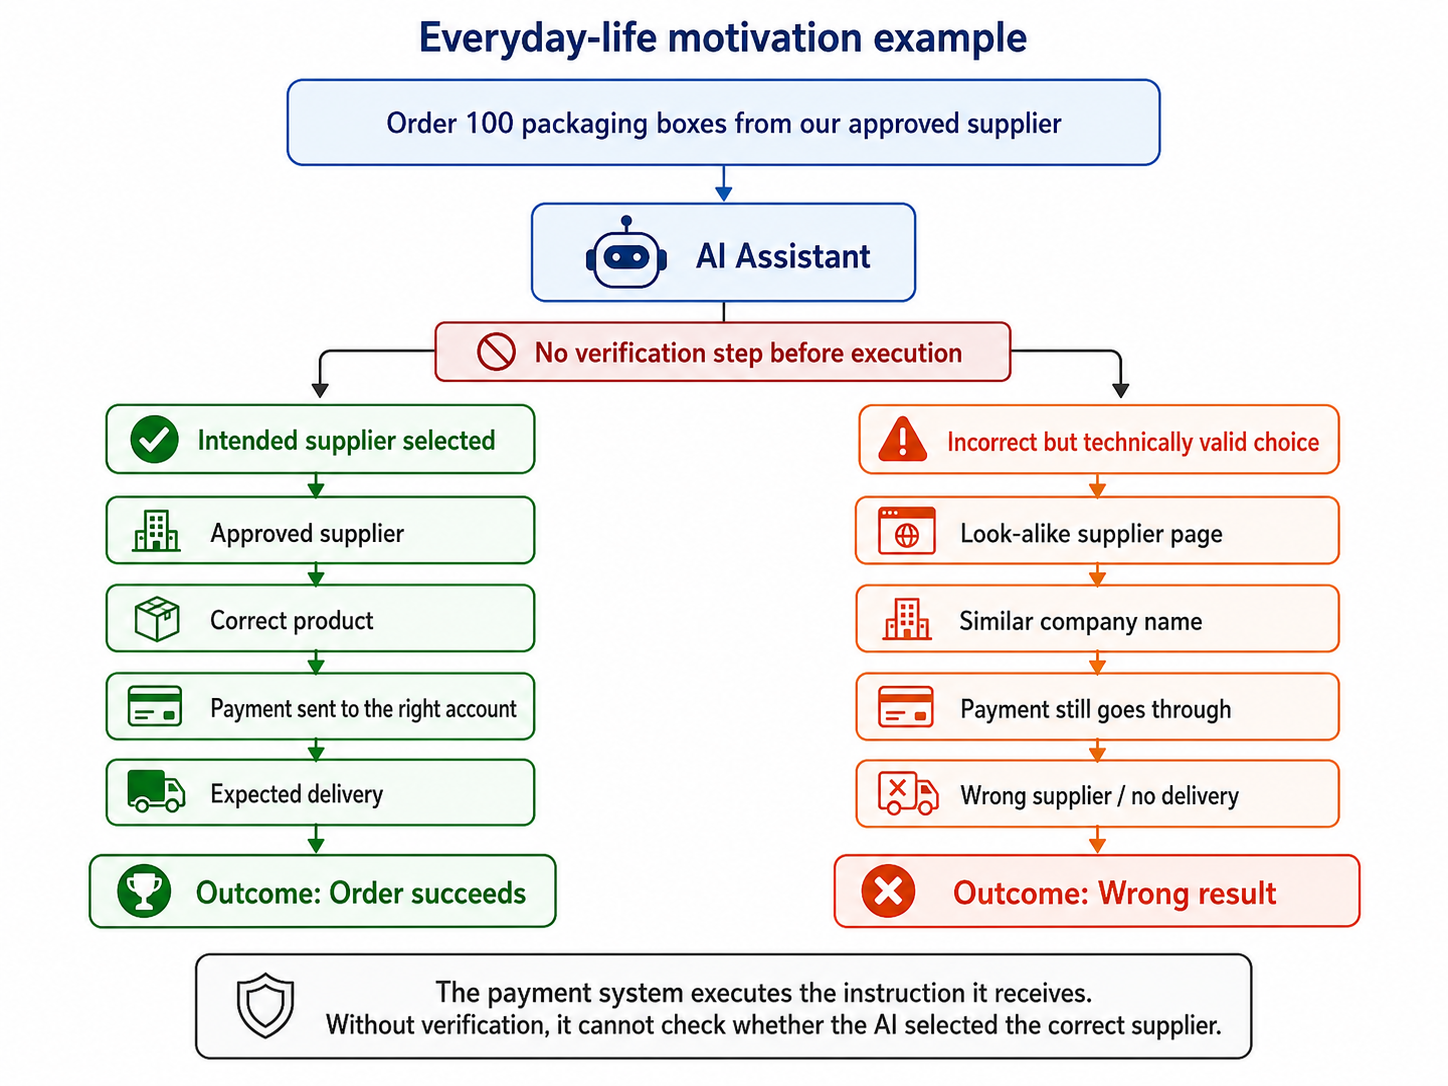
\includegraphics[width=0.88\textwidth]{figures/motivation_scenario.png}
%     \caption{An AI assistant may select either the intended supplier or an incorrect but technically valid supplier when no independent verification step is applied.(generated by GPT)}
%     \label{fig:motivation_scenario}
% \end{figure}

% The same situation can occur in DeFi. Consider the instruction:

% \begin{quote}
% \textit{``Supply 100 USDT to Aave\footnote{Aave is an Open Source Protocol to create Non-Custodial Liquidity Markets to earn interest on supplying and borrowing assets with a variable interest rate.} V3.''}
% \end{quote}

% The user expects a specific financial result: 100 USDT should be supplied to the intended Aave V3 market. To carry out this request, several technical elements must eventually correspond to each other. The operation must involve the correct protocol deployment, the requested action, an appropriate smart contract, a function capable of performing that action, and a supported USDT reserve.

% A transaction containing incorrect execution information may nevertheless be technically valid. It may be correctly encoded, digitally signed, accepted by a smart contract, and included in the blockchain. Technical execution therefore does not by itself establish that the transaction reflects the user's original request.

% This distinction is especially relevant in blockchain systems because confirmed transactions are difficult to reverse. A mistake involving the wrong contract, token, recipient, or function can therefore have direct financial consequences.

% The motivation for this thesis is not to replace existing wallet security, transaction simulation, digital signatures, or smart-contract security mechanisms. These mechanisms address important aspects of blockchain security. The motivation is to address a different question:

% \begin{quote}
% \textit{Does the transaction that is about to be constructed correspond to the DeFi action that the user actually requested?}
% \end{quote}

% Answering this question before execution would allow AI-assisted DeFi systems to combine the usability of natural-language interaction with an additional check of the intended execution relationship.

\section{Motivation}
\label{sec:motivation}

An AI assistant can prepare an instruction that a payment system accepts
even when the funds are directed to the wrong destination. Consider
\textit{BrightCart Studio}, a small online business whose employee asks
an assistant to ``order 100 packaging boxes from our approved supplier.'' BrightCart's supplier record identifies Account A as the registered
payment account for Supplier A. As Figure~\ref{fig:motivation_scenario}
shows, the assistant selects Supplier A but enters Account B in the
payment instruction. If Account B can receive the payment and the
instruction passes the payment system's checks, the payment may be
processed. The error lies in the association between the supplier and
the account selected for payment.

\begin{figure}[H]
    \centering
    % \begingroup
% \definecolor{motfill}{HTML}{F8FAFC}
% \definecolor{motborder}{HTML}{475569}
% \definecolor{motarrow}{HTML}{64748B}
% \definecolor{mottext}{HTML}{1E293B}
% \definecolor{motaccent}{HTML}{9A4A32}
% \begin{tikzpicture}[
%     >=stealth,
%     font=\sffamily\fontsize{10}{12}\selectfont,
%     box/.style={draw=motborder, fill=motfill, text=mottext,
%         line width=0.6pt, rounded corners=2pt,
%         align=center, inner xsep=8pt, inner ysep=9pt},
%     panel/.style={box, text width=5.4cm, minimum height=2.9cm},
%     flow/.style={->, draw=motarrow, line width=0.85pt,
%         shorten <=2pt, shorten >=2pt},
%     compare/.style={->, draw=motarrow, line width=0.85pt,
%         shorten <=2pt, shorten >=2pt},
%     icon/.style={draw=motborder, line width=0.8pt,
%         line cap=round, line join=round},
%     pics/person/.style={code={
%         \draw[icon] (0,0.12) circle (0.11);
%         \draw[icon] (-0.22,-0.22) .. controls (-0.22,0.02)
%             and (0.22,0.02) .. (0.22,-0.22) -- cycle;
%     }},
%     pics/record/.style={code={
%         \draw[icon] (-0.18,-0.23) rectangle (0.18,0.23);
%         \foreach \y in {-0.12,0,0.12}
%             \draw[icon] (-0.10,\y) -- (0.10,\y);
%     }},
%     pics/ai/.style={code={
%         \draw[icon,rounded corners=1pt]
%             (-0.18,-0.18) rectangle (0.18,0.18);
%         \foreach \p in {-0.09,0.09}{
%             \draw[icon] (\p,0.18) -- (\p,0.27);
%             \draw[icon] (\p,-0.18) -- (\p,-0.27);
%             \draw[icon] (0.18,\p) -- (0.27,\p);
%             \draw[icon] (-0.18,\p) -- (-0.27,\p);
%         }
%         \node[text=motborder,font=\sffamily\tiny] at (0,0) {AI};
%     }},
%     pics/mismatch/.style={code={
%         \draw[icon,draw=motaccent] (0,0) circle (0.23);
%         \draw[icon,draw=motaccent] (-0.11,0.06) -- (0.11,0.06);
%         \draw[icon,draw=motaccent] (-0.11,-0.06) -- (0.11,-0.06);
%         \draw[icon,draw=motaccent] (-0.07,-0.15) -- (0.07,0.15);
%     }},
%     pics/payment/.style={code={
%         \draw[icon,rounded corners=1pt]
%             (-0.28,-0.18) rectangle (0.28,0.18);
%         \draw[icon] (-0.28,0.05) -- (0.28,0.05);
%         \draw[icon] (-0.19,-0.09) -- (-0.04,-0.09);
%     }}
% ]
% \node[box, text width=11.9cm] (request) at (0,0)
%     {\rule{0pt}{0.48cm}\\[2pt]\textbf{Employee request}\\[4pt]
%     ``Order 100 packaging boxes from our approved supplier.''};

% \node[panel] (record) at (-3.25,-3.25)
%     {\rule{0pt}{0.48cm}\\[2pt]\textbf{Approved supplier record}\\[7pt]
%     Supplier A\\[4pt]
%     Registered account: \textbf{Account A}};

% \node[panel] (candidate) at (3.25,-3.25)
%     {\rule{0pt}{0.48cm}\\[2pt]\textbf{AI payment instruction}\\[7pt]
%     Supplier A\\[4pt]
%     Selected account: \textcolor{motaccent}{\textbf{Account B}}};

% \pic at ([yshift=-0.40cm]request.north) {person};
% \pic at ([yshift=-0.45cm]record.north) {record};
% \pic at ([yshift=-0.45cm]candidate.north) {ai};

% \draw[flow] (request.south -| record.north) -- (record.north);
% \draw[flow] (request.south -| candidate.north) -- (candidate.north);

% \node[box, draw=motaccent, text width=11.9cm] (mismatch) at (0,-6.2)
%     {\rule{0pt}{0.48cm}\\[2pt]\textbf{Account mismatch}};

% \pic at ([yshift=-0.40cm]mismatch.north) {mismatch};

% \draw[compare] (record.south) -- (record.south |- mismatch.north);
% \draw[compare] (candidate.south) -- (candidate.south |- mismatch.north);

% \node[box, text width=11.9cm] (consequence) at (0,-8.75)
%     {\rule{0pt}{0.48cm}\\[2pt]\textbf{Without verification}\\[4pt]
%     Payment may reach the wrong account.};
% \pic at ([yshift=-0.40cm]consequence.north) {payment};
% \draw[flow] (mismatch.south) -- (consequence.north);
% \end{tikzpicture}
% \endgroup

% Requires \usepackage{tikz}. Drawing only; keep the figure
% environment and its label in the introduction chapter.
\begingroup
\definecolor{motborder}{HTML}{475569}
\definecolor{motfill}{HTML}{F8FAFC}
\definecolor{mottext}{HTML}{1E293B}
\definecolor{motaccent}{HTML}{914832}

\begin{tikzpicture}[
    x=1cm, y=1cm,
    font=\sffamily\small,
    every node/.style={text=mottext, inner sep=0pt}
]
% The request provides context for both columns.
\node[align=center, text width=11.4cm] at (0,0)
    {``Order 100 packaging boxes from our approved supplier.''};

% Comparison table: fields at left, expected and proposed values at right.
\fill[motfill] (-5.7,-0.60) rectangle (5.7,-1.65);
\draw[motborder, line width=0.7pt]
    (-5.7,-0.60) -- (5.7,-0.60)
    (-5.7,-1.65) -- (5.7,-1.65)
    (-5.7,-3.05) -- (5.7,-3.05);

\node[anchor=west, font=\sffamily\small\bfseries]
    at (-5.45,-1.12) {Field};
\node[align=center] at (-0.55,-1.12)
    {\textbf{Expected}\\Company record};
\node[align=center] at (3.48,-1.12)
    {\textbf{Actual proposal}\\AI payment instruction};

\node[anchor=west] at (-5.45,-2.03) {Supplier};
\node at (-0.55,-2.03) {Supplier A};
\node at (3.48,-2.03) {Supplier A};

\node[anchor=west] at (-5.45,-2.70) {Payment account};
\node at (-0.55,-2.70) {\textbf{Account A}};
\node[text=motaccent] at (3.48,-2.70) {\textbf{Account B}};
\end{tikzpicture}
\endgroup
    \caption{BrightCart's registered payment details and the assistant's
    proposal.}
    \label{fig:motivation_scenario}
\end{figure}

In DeFi, the corresponding question is whether the selected contract
belongs to the intended market. Consider the request:

\begin{quote}
\textit{``Supply 100 USDT to Aave V3.''}\footnote{Aave is a
decentralised liquidity protocol that supports supplying and borrowing
cryptoassets. For an empirical study of lending markets including Aave,
see Gudgeon et al.~\cite{gudgeonLoanableFunds2020}. For the Aave V3 Pool
contract, see \url{https://aave.com/docs/aave-v3/smart-contracts/pool}.}
\end{quote}

The request specifies the action, asset, and amount, but leaves the
network and market unstated. Suppose the execution context identifies
the network and Market A as the intended Aave V3 market. The supply
operation then requires the Pool contract for Market A, its supply
function, and the USDT reserve supported by that market.

In Figure~\ref{fig:aave_supply_comparison}, the assistant preserves
the instruction to supply 100 USDT but selects Pool B, which belongs
to Market B on the same network. If Market B supports the same token
and the call meets its execution conditions, the transaction could
succeed. The funds would then be supplied to Market B even though
Market A was intended.

\begin{figure}[htbp]
    \centering
    % Drawing only. Requires \usepackage{tikz}.
\begingroup
\definecolor{motInk}{HTML}{1E293B}
\definecolor{motRule}{HTML}{475569}
\definecolor{motLight}{HTML}{F1F5F9}
\definecolor{motRust}{HTML}{853E2D}
\begin{tikzpicture}[x=1cm,y=1cm,font=\sffamily\small,
every node/.style={text=motInk,inner sep=0pt}]
\node[align=center,font=\sffamily\bfseries] at (0,0)
  {\textquotedblleft Supply 100 USDT to Aave V3.\textquotedblright};
\node[align=center,font=\sffamily\small] at (0,-.52)
  {Execution context: intended market A};
\fill[motLight] (-5.7,-.98) rectangle (5.7,-1.85);
\draw[motRule,line width=.65pt] (-5.7,-.98)--(5.7,-.98)
 (-5.7,-1.85)--(5.7,-1.85) (-5.7,-3.93)--(5.7,-3.93);
\node[anchor=west,font=\sffamily\small\bfseries] at (-5.45,-1.42) {Field};
\node[align=center] at (-.45,-1.42) {\textbf{Expected}\\Market record};
\node[align=center] at (3.52,-1.42) {\textbf{Proposed}\\AI instruction};
\node[anchor=west] at (-5.45,-2.21) {Operation};
\node at (-.45,-2.21) {Supply 100 USDT};
\node at (3.52,-2.21) {Supply 100 USDT};
\node[anchor=west] at (-5.45,-2.87) {Target contract};
\node at (-.45,-2.87) {\textbf{Pool A}};
\node[text=motRust] at (3.52,-2.87) {\textbf{Pool B}};
\node[anchor=west] at (-5.45,-3.53) {Market of target};
\node at (-.45,-3.53) {Market A};
\node[text=motRust] at (3.52,-3.53) {Market B};
\end{tikzpicture}
\endgroup
    \caption{Expected and proposed Pool contracts for the same Aave V3
    supply request.}
    \label{fig:aave_supply_comparison}
\end{figure}

Related work illustrates why the identity behind an address matters.
Tsuchiya et al.\ document transfers to unintended addresses that
resembled those of familiar recipients
\cite{tsuchiyaAddressPoisoning2025}. Gallersd\"orfer et al.\ examine
how a wallet can verify the association between a website and a
contract address \cite{gallersdorferMetaMaskTLS2022}. The Aave example
requires a distinct check: even a legitimate Pool contract can be
inappropriate for a request if it belongs to a different market.

This thesis complements wallet controls, transaction simulation,
digital signatures, and smart-contract security analysis by asking
the following question before transaction construction:

\begin{quote}
\textit{Does authoritative information for the selected network and
market support the execution relationships required by the proposed
DeFi operation?}
\end{quote}

Approval means that the mandatory relationships for the structured
operation have been established within the supported scope. It does
not establish that the assistant interpreted the original request
correctly, guarantee successful execution, or predict a favourable
financial outcome. If the evidence is incomplete or outdated to the
extent that a required relationship cannot be established, the
operation must not be approved.

% \section{Problem Analysis}
% \label{sec:problem_analysis}

% The motivating example represents one instance of a broader problem. AI-driven DeFi workflows contain several stages at which incomplete, incorrect, or mismatched information can influence the final transaction. Research on autonomous blockchain agents identifies related risks involving intent formulation, delegated execution, authorization, policy misuse, and transaction pipelines \cite{alqithamiAutonomousAgentsBlockchains2026}.

% The main sub-problems relevant to this thesis are described below.


% \subsection{Natural-Language Requests Can Be Incomplete or Ambiguous}
% \label{subsec:natural_language_problem}

% Users normally describe financial actions in ordinary language rather than through complete blockchain transaction parameters.

% For example:

% \begin{quote}
% ``Swap WETH for USDT.''
% \end{quote}

% This request does not specify an amount, blockchain network, protocol deployment, or other action-specific information.

% Similarly:

% \begin{quote}
% ``Supply USDT to Aave.''
% \end{quote}

% does not specify the amount, network, Aave market, or exact asset representation.

% An AI agent may attempt to infer missing information. However, an automatically inferred value may differ from what the user intended. A secure workflow must therefore distinguish information that describes the user's financial intention from technical information that can be resolved later. Critical ambiguity must not silently become part of an executable financial operation.


% \subsection{AI-Generated Information Can Be Plausible but Incorrect}
% \label{subsec:probabilistic_ai_problem}

% LLMs are useful for interpreting natural language, but their outputs are probabilistic. A generated result may appear clear and technically convincing while still containing incorrect or mismatched information. Retrieval-Augmented Generation can improve access to external and more current information, but retrieval does not automatically guarantee that the retrieved information is authoritative, complete, or correctly interpreted. The final result may still contain an incorrect protocol, action, asset, address, or function.

% This creates a security problem when the same generated information is used directly to construct a financial transaction. The correctness of an AI-generated action should therefore not depend only on the confidence or plausibility of the language-model output.


% \subsection{DeFi Actions Require Different Execution Relationships}
% \label{subsec:action_specific_problem}

% Different DeFi operations require different \textbf{execution relationships}. 
% For example, a \textit{token swap} typically connects an input asset and an output asset with an exchange protocol, router contract, swap function, and supported liquidity pool or token pair. 
% A \textit{lending operation}, in contrast, connects a lending protocol with a supported reserve asset, protocol contract, action-specific function, and amount. 
% Therefore, the required verification depends on the \textbf{type of DeFi action} being performed. Transfers and token approvals require different information again.

% Therefore, verifying only one isolated value is insufficient. For example, confirming that a contract belongs to Aave does not prove that it is the correct contract for the requested action. Likewise, confirming that USDT is a known token does not prove that it is supported by the selected protocol deployment.

% The relevant entities must form the correct action-specific execution relationship.


% \subsection{Human-Readable Names Are Not Sufficient Identifiers}
% \label{subsec:identifier_problem}

% Users naturally refer to protocols and assets using names such as ``Aave'', ``Uniswap'', ``USDT'', or ``WETH''. Blockchain execution, however, ultimately depends on network-specific contract addresses, functions, and encoded parameters. A token symbol may exist on several blockchain networks, and different contracts may use identical or similar names. A contract may also use terminology associated with a well-known protocol without belonging to an official deployment.

% Consequently, a correct interpretation at the language level does not automatically provide an authoritative blockchain identifier. The relationship between human-readable intent and the corresponding on-chain entities must be established before execution.


% \subsection{Authorization and Intent Correctness Are Different Problems}
% \label{subsec:authorization_problem}

% Programmable wallets can restrict the actions available to an automated agent. For example, a wallet may limit the maximum amount that can be spent or restrict transactions to selected contracts. ERC-4337 and related programmable-account mechanisms provide an important basis for such controlled execution \cite{buterinERC4337AccountAbstraction2021,
% linMeasurementInvestigationERC43372024}.

% These mechanisms primarily answer an authorization question:

% \begin{quote}
% ``Is this agent permitted to execute this operation?''
% \end{quote}

% However, authorization does not necessarily answer:

% \begin{quote}
% ``Is this operation the correct interpretation of the user's request?''
% \end{quote}

% For example, an agent may have permission to interact with both Uniswap and Aave. If it prepares a Uniswap swap when the user requested an Aave supply action, the operation could remain within the wallet's permissions while still being inconsistent with the user's intention.

% Authorization and intent correctness must therefore be treated as separate concerns.


% \subsection{Verification Depends on Current and Authoritative Information}
% \label{subsec:trusted_information_problem}

% The correctness of a DeFi execution path depends on information about protocol deployments, smart contracts, callable functions, pools, reserves, assets, and blockchain networks. This information may change. Protocols can introduce new deployments, add supported assets, update integrations, or deprecate earlier components. Information that was once correct may therefore become outdated.

% A verification mechanism that uses outdated or untrusted information can produce incorrect decisions even when its internal checking process behaves consistently. The source and freshness of verification information are therefore part of the problem itself.


% \subsection{Problem Statement}
% \label{subsec:problem_statement}

% The preceding sub-problems lead to the central problem addressed by this thesis:

% \begin{quote}
% \textbf{The problem addressed in this thesis is how to verify, before blockchain execution, that an AI-generated DeFi transaction intent is consistently mapped to the intended protocol deployment, action, authoritative smart contract, callable function, and supported asset or protocol resource.}
% \end{quote}

% Figure~\ref{fig:problem_statement_overview} summarises the position of this problem within an AI-driven DeFi workflow.

% \begin{figure}[htbp]
%     \centering
%     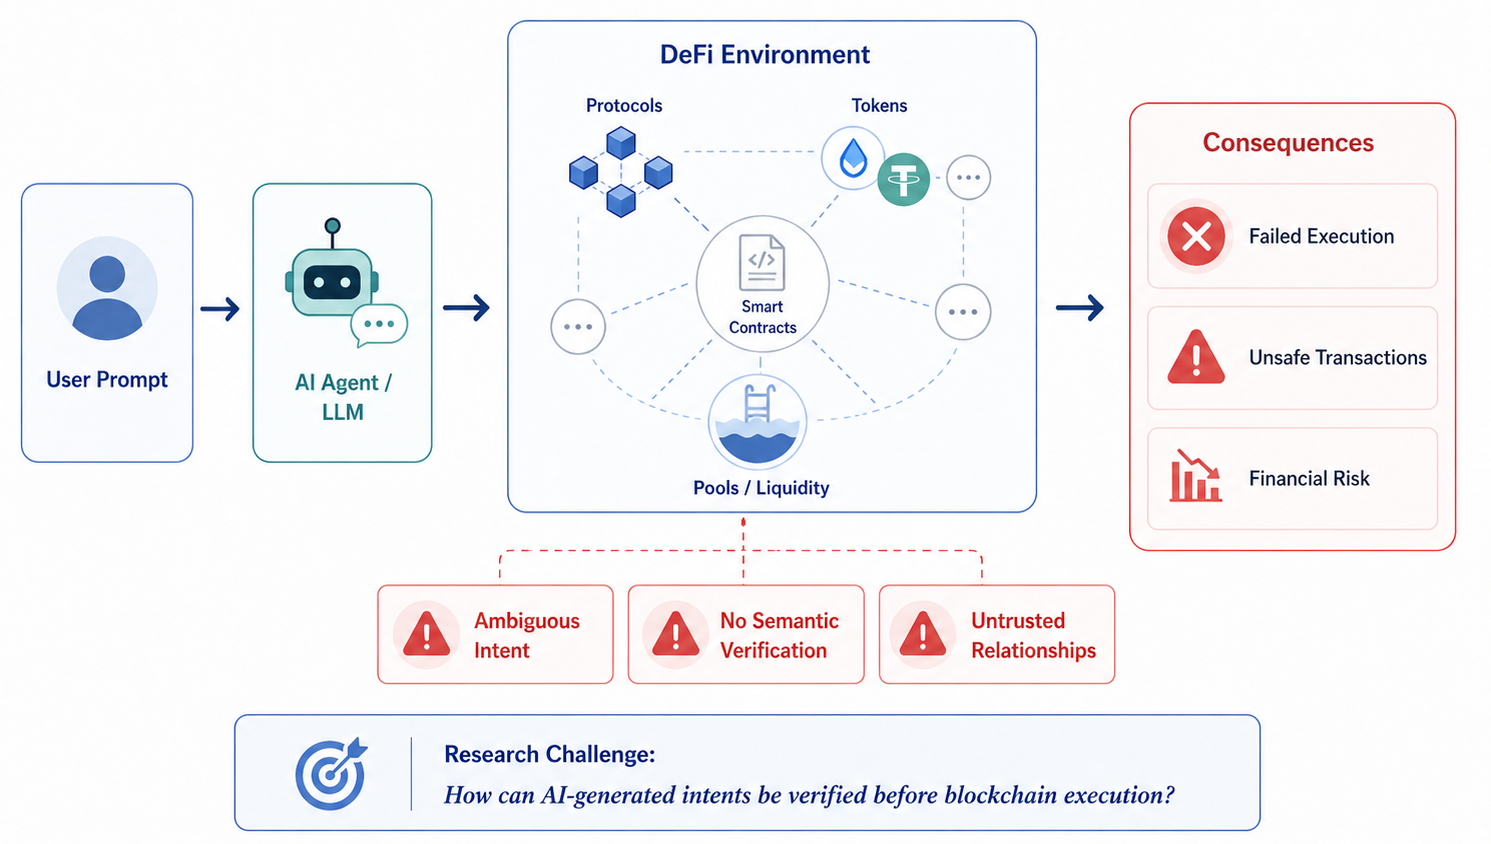
\includegraphics[width=0.90\textwidth]{figures/problem_statement_overview.png}
%     \caption{The verification problem investigated between AI-generated DeFi intent and blockchain transaction construction.(generated by GPT)}
%     \label{fig:problem_statement_overview}
% \end{figure}

% The problem is located after the user's request has been interpreted but before the corresponding blockchain transaction is constructed and executed. The required check concerns not only individual entities, but also whether those entities form the correct relationship for the requested financial action.
\section{Problem Analysis}
\label{sec:problem_analysis}

% Bold, unnumbered headings on their own line; keep each with its paragraph.
\providecommand{\problemheading}[1]{%
  \par\addvspace{0.8\baselineskip}%
  \noindent\textbf{#1}\par\nobreak\smallskip\nobreak
  \noindent\ignorespaces}

The supply example illustrates how an assistant can preserve the requested
action and amount yet select a contract belonging to the wrong market.
Research on autonomous blockchain agents identifies related risks in intent
formulation, delegated execution, authorisation, and transaction preparation
\cite{alqithamiAutonomousAgentsBlockchains2026}. The first three subproblems concern incomplete or ambiguous requests,
plausible but incorrect model outputs, and execution relationships that
cannot be verified by checking entities in isolation. The remaining three
concern the difficulty of resolving names to on-chain identifiers, the
limits of wallet authorisation as evidence of user intent, and the
reliability of the information used for verification.

\problemheading{Incomplete or ambiguous requests}
A request can be incomplete even when the intended action is clear.
Consider the instruction:

\begin{quote}
\textit{``Swap WETH for USDT.''}
\end{quote}

The user has specified the swap direction but has not said how much WETH
to exchange. Identifying the appropriate deployment or pool cannot resolve
that omission. By contrast, consider a request that specifies the amount:

\begin{quote}
\textit{``I need 100 USDT from Aave.''}
\end{quote}

Here the uncertainty concerns the action. Depending on the user's position,
the request could mean withdrawing previously supplied USDT or borrowing
USDT. Both could put the same amount in the user's wallet, but withdrawing
reduces a supplied balance, whereas borrowing creates a debt. If the
context does not distinguish these intentions, the assistant must seek
clarification or stop before preparing the operation. Technical details present a different case. Once the action and execution
context are established, contract addresses can be resolved from
authoritative information. An explicit application policy may also supply
a default network when the user omits it, but must not override a network
the user specifies.

\problemheading{Plausible but incorrect AI interpretations}
LLMs are useful for interpreting natural language, but their outputs
are probabilistic. A generated result may appear clear and technically
convincing while containing incorrect or mismatched information.
Retrieval-Augmented Generation can improve access to external
information, including information that is more recent than the model's
training data. However, retrieval does not automatically establish that
the information is authoritative, complete, current, or correctly
interpreted. The generated result may still contain an incorrect
protocol, action, asset, address, or function.

This creates a security problem when generated information is used
directly to construct a financial transaction. A plausible explanation
or a structurally valid output does not establish that the proposed
operation is supported by the selected protocol deployment. The
correctness of an AI-generated action should therefore not depend
solely on the apparent confidence or plausibility of the model's output. Two forms of correctness must be distinguished. The first concerns
whether the structured intent accurately represents the user's request.
The second concerns whether the execution relationships required by
that intent can be established from authoritative information. An
incorrectly interpreted request may still describe an operation with
valid execution relationships. Interpretation correctness and
relationship verification must therefore be assessed separately.


\problemheading{Valid entities with incompatible execution relationships}
For a token swap, the selected contract and function must support the
exchange, and the chosen pool or route must connect the input and output
assets. For a lending operation, the contract must belong to the selected
market, the function must perform the requested action, and the asset must
correspond to a supported reserve. A function that borrows an asset cannot
serve a request to repay it, even if both functions belong to the same
contract. Checking each entity independently misses this distinction. A Pool contract
may belong to Aave V3 and a token contract may identify USDT on the
selected network, yet the Pool may belong to another market or may not
support that reserve. Verification must therefore establish the
relationships required by the particular action and deployment.

\problemheading{Ambiguous protocol and asset identifiers}
Users naturally refer to protocols and assets using names such as
``Aave'', ``Uniswap'', ``USDT'', or ``WETH''. Blockchain execution,
however, depends on network-specific contract addresses, functions,
and encoded parameters. A token symbol may be used on several
blockchain networks, and different contracts may use identical or
similar names. A contract may also use terminology associated with a
well-known protocol without belonging to an official deployment. Consequently, a correct interpretation of a name at the language level
does not provide an authoritative blockchain identifier. Resolving
``USDT'', for example, requires identifying the relevant token contract
within the applicable network and establishing its relationship to
the selected protocol resource.

The mapping from human-readable intent to on-chain entities must
therefore be grounded in authoritative information. A matching name
alone is insufficient evidence that a contract, asset, or protocol
resource is appropriate for the requested operation.


\problemheading{Wallet permissions do not establish user intent}
Programmable wallets can restrict the actions available to an automated
agent. Depending on their implementation, wallet policies may limit
spending amounts or restrict interactions to selected contracts.
ERC-4337 and related programmable-account mechanisms provide a basis
for implementing such controlled execution
\cite{buterinERC4337AccountAbstraction2021,
linMeasurementInvestigationERC43372024}.

These controls address an authorisation question:

\begin{quote}
\textit{``Is this agent permitted to execute this operation?''}
\end{quote}

Authorisation does not necessarily answer:

\begin{quote}
\textit{``Does this operation correspond to the user's request?''}
\end{quote}

For example, an agent may have permission to interact with both Uniswap
and Aave. If it prepares a Uniswap swap when the user requested an Aave
supply action, the operation could remain within the wallet's
permissions while being inconsistent with the user's intention. This example also illustrates the boundary of relationship
verification. If the incorrectly generated swap intent describes a
supported Uniswap operation, its execution relationships may be valid.
Checking those relationships alone would not reveal that the user
originally requested a different action.

Interpretation correctness, relationship verification, and execution
authorisation must therefore be treated as separate concerns. Within
this distinction, the central verification task of this thesis is to
establish whether the structured DeFi intent is consistent with the
authoritative execution relationships required for the proposed
operation.


\problemheading{Outdated or incomplete verification evidence}
The correctness of a DeFi execution structure depends on information
about protocol deployments, smart contracts, callable functions, pools,
reserves, assets, and blockchain networks. This information may change.
Protocols can introduce new deployments, add supported assets, update
integrations, or deprecate earlier components. Information that was
once correct may therefore become outdated. A verification mechanism that relies on outdated or untrusted
information can produce incorrect decisions even when its internal
checking process behaves consistently. The source and freshness of
verification knowledge are therefore part of the problem itself. Completeness is also relevant. If a required relationship is absent
from the available knowledge, this absence does not necessarily
establish that the operation is unsupported. It may instead indicate
incomplete coverage or a failed acquisition or update process.
Treating an absent relationship as evidence of an unsupported operation
requires sufficiently complete and current knowledge for the relevant
verification scope.

The verification process must therefore distinguish evidence of an
unsupported or inconsistent operation from insufficient evidence to
reach a decision. When the required relationships cannot be established
reliably, the operation must not be approved.


\problemheading{Problem statement}
These subproblems lead to the central question of this thesis:

\begin{quote}
\textbf{Before a transaction is constructed, how can a verifier establish
whether authoritative information supports the relationships that an
AI-generated structured DeFi intent requires among the network, protocol
deployment, action, contract, function, and relevant assets, pools, or
reserves?}
\end{quote}

Figure~\ref{fig:problem_statement_overview} shows where a mismatch can
pass unnoticed if a structured intent is used directly for transaction
construction. The solid arrows show the processing sequence. The
annotation marks the transition at which evidence for the proposed
relationships is needed. If a mismatch goes unchecked, the transaction
may fail, or it may execute against an unintended target.

\begin{figure}[H]
    \centering
    \begingroup
\definecolor{probfill}{HTML}{F8FAFC}
\definecolor{probborder}{HTML}{475569}
\definecolor{probtext}{HTML}{1E293B}
\definecolor{probaccent}{HTML}{984A35}
\definecolor{probgap}{HTML}{FCF8F6}
\begin{tikzpicture}[
    >=stealth,
    font=\sffamily\fontsize{10}{12}\selectfont,
    box/.style={draw=probborder,fill=probfill,text=probtext,
      rounded corners=2pt,line width=0.6pt,align=center,
      inner xsep=7pt,inner ysep=8pt},
    flow/.style={->,draw=probborder,line width=0.75pt,
      shorten <=2pt,shorten >=2pt},
    icon/.style={draw=probborder,line width=0.8pt,line cap=round,
      line join=round},
    pics/person/.style={code={
      \draw[icon] (0,0.15) circle (0.12);
      \draw[icon] (-0.24,-0.22) .. controls (-0.24,0.05)
        and (0.24,0.05) .. (0.24,-0.22);
      \draw[icon] (-0.24,-0.22)--(0.24,-0.22);
    }},
    pics/chip/.style={code={
      \draw[icon,rounded corners=1pt] (-0.2,-0.2) rectangle (0.2,0.2);
      \foreach \p in {-0.1,0.1}{
        \draw[icon] (\p,0.2)--(\p,0.29);
        \draw[icon] (\p,-0.2)--(\p,-0.29);
        \draw[icon] (0.2,\p)--(0.29,\p);
        \draw[icon] (-0.2,\p)--(-0.29,\p);
      }
      \node[text=probborder,font=\sffamily\tiny] at (0,0) {AI};
    }},
    pics/document/.style={code={
      \draw[icon] (-0.18,-0.25)--(0.18,-0.25)--(0.18,0.13)
        --(0.06,0.25)--(-0.18,0.25)--cycle;
      \draw[icon] (0.06,0.25)--(0.06,0.13)--(0.18,0.13);
      \foreach \p in {-0.12,-0.02,0.08}
        \draw[icon] (-0.10,\p)--(0.09,\p);
    }},
    pics/blocks/.style={code={
      \draw[icon] (-0.4,-0.12) rectangle (-0.16,0.12);
      \draw[icon] (-0.12,-0.12) rectangle (0.12,0.12);
      \draw[icon] (0.16,-0.12) rectangle (0.4,0.12);
      \draw[icon] (-0.16,0)--(-0.12,0);
      \draw[icon] (0.12,0)--(0.16,0);
    }}
]
% Only the five stages use boxes and arrows. The note is a margin annotation.
\foreach \id/\x/\glyph/\title in {
    req/0/person/{User\\request},interp/2.68/chip/{AI\\interpretation},
    cand/5.36/document/{Structured\\intent},build/8.64/document/{Transaction\\construction},
    exec/11.32/blocks/{Blockchain\\execution}}{
    \node[box,minimum width=2.20cm,minimum height=1.54cm] (\id) at (\x,0) {};
    \pic at (\x,0.43) {\glyph};
    \node[align=center,text=probtext,font=\sffamily\bfseries\fontsize{9}{10.2}\selectfont]
        at (\x,-0.24) {\title};
}
\draw[flow] (req.east)--(interp.west);
\draw[flow] (interp.east)--(cand.west);
\draw[flow] (cand.east)--(build.west);
\draw[flow] (build.east)--(exec.west);

% Non-directional leader touches the transition, not either stage.
\draw[draw=probaccent,densely dashed,line width=0.65pt]
    (7.00,-0.05)--(7.00,-1.08);
\node[anchor=north,text=probaccent,font=\sffamily\bfseries\small]
    at (7.00,-1.11) {verification gap};
\node[anchor=north,align=center,text=probtext,font=\sffamily\small]
    at (7.00,-1.66) {If a required relationship is left unchecked, a mismatch can\\
                      cause execution to fail or the wrong operation to succeed.};
\end{tikzpicture}
\endgroup
    \caption[Verification gap before transaction construction]{Verification gap before transaction construction in DeFi.}
    \label{fig:problem_statement_overview}
\end{figure}

The proposed verifier addresses this gap by checking the structured intent
against authoritative knowledge. Approval requires evidence for every
mandatory relationship within the supported scope. An established
mismatch and insufficient evidence both prevent the operation from
proceeding, although they are distinct findings. Only an approved
structured verification result may be used to construct the transaction;
the execution component must not reconstruct the operation from the
original request. Approval neither establishes that the model interpreted
the request correctly nor guarantees successful execution or a favourable
financial outcome.


\section{Objectives and Scope}
\label{sec:objectives_scope}

The main objective of this thesis is to investigate whether an
automatically populated, domain-specific property graph can verify the
execution relationships required by an AI-generated DeFi intent before
transaction construction, and how the resulting decision can be used
in a controlled ERC-4337 wallet workflow.

Research on knowledge graphs and large language models examines how
explicit relationships can support the use of external knowledge
\cite{panUnifyingLargeLanguage2024}. Graph-based retrieval approaches
also use these relationships to retrieve information across connected
entities \cite{hanRetrievalAugmentedGenerationGraphs2025,
hanRAGVsGraphRAG2026}. In this thesis, the graph serves a different
purpose: it provides the evidence against which a proposed operation
is checked.

The six sub-objectives below correspond, in order, to the six
sub-problems identified in Section~\ref{sec:problem_analysis}:

\begin{enumerate}
    \item \textbf{Identify missing or ambiguous intent information.}
    Translate selected natural-language requests into machine-readable
    intents and distinguish information established by the request or
    the configured execution context from information that still
    requires clarification.

    \item \textbf{Check AI-generated proposals against independent
    evidence.}
    Assess the operation proposed by the assistant against protocol
    and blockchain information obtained independently of the language
    model. A plausible interpretation is not sufficient grounds for
    approval.

    \item \textbf{Verify the relationships required by each action.}
    Represent and check how the deployment, contract, function, and
    assets must be connected for the proposed action, including the
    relevant pool or reserve where applicable. The presence of each
    entity in the graph is insufficient if the required connections
    do not hold.

    \item \textbf{Resolve names to identifiers on the selected network.}
    Establish which deployment, contract, and token identifiers
    correspond to the protocol and asset names used in a structured
    intent. This allows the verifier to distinguish entities that
    share a name or symbol.

    \item \textbf{Distinguish intent verification from wallet
    authorisation.}
    Investigate how a controlled ERC-4337 wallet workflow can use the
    verification result so that only an approved operation proceeds
    to transaction construction. Permission to call a contract does
    not, by itself, establish that the contract is appropriate for
    the requested action.

    \item \textbf{Account for the source, freshness, and completeness
    of verification evidence.}
    Automatically populate the graph from configured authoritative
    sources and distinguish evidence of a mismatch from a case in
    which the available information is too incomplete or outdated
    to support a decision.
\end{enumerate}

The evaluation assesses these objectives across supported and
unsupported operations. It examines verification effectiveness,
repeatability, decision traceability, processing time, and the extent
to which the graph can be extended without redesigning the
verification model.

\medskip
\noindent\textbf{Scope.}
The prototype is evaluated on Ethereum Sepolia and covers two protocols
with different execution relationships. For Uniswap V3, it considers
single-hop token swaps, for which the selected router and swap function
must support the operation and the pool must correspond to the
requested token pair. For Aave V3, it considers supply, withdrawal,
borrowing, and repayment, for which the selected Pool contract,
function, and reserve asset must correspond to the intended market
and action. The asset scope includes USDT and WETH. Protocol-specific ingestion components populate the graph with the
entities and relationships needed for these operations. The bounded
scope makes it possible to document the expected relationships and
test both supported execution paths and cases involving an incorrect
contract, an unsupported asset or protocol-action combination, or
missing evidence. Extensibility is examined by adding entities or
relationships within this model.

\medskip
\noindent\textbf{Meaning and limits of approval.}
The verifier distinguishes three outcomes. \texttt{APPROVE} means
that the available authoritative evidence supports the mandatory
relationships for the structured operation in the selected context.
\texttt{REJECT} means that the evidence establishes a mismatch.
\texttt{INSUFFICIENT\_EVIDENCE} means that a required relationship
cannot be established from sufficiently complete and current
information. Only \texttt{APPROVE} permits the operation to proceed. Approval applies to the structured intent submitted for verification.
It does not establish that the assistant captured every aspect of the
user's original request: an incorrectly interpreted action may itself
have valid execution relationships. Approval also does not guarantee
successful execution, a favourable financial outcome, or the absence
of vulnerabilities in a protocol contract.

The thesis does not attempt to cover the entire DeFi ecosystem,
provide investment advice, audit or formally verify protocol
implementations, or enable unrestricted trading with real funds on
production networks. Compromised wallets or devices, stolen keys,
manipulated oracles, and attacks on the assistant's reasoning process
are also outside its scope. An operation produced through prompt
injection may fail the relationship checks, but the verifier does not
detect prompt injection itself.


\section{Outline of the Thesis}
\label{sec:thesis_structure}

The remainder of the thesis follows the argument established in this chapter.\\ Chapter~\ref{chap:stateoftheart} first derives the requirements that follow from the identified problem and examines how existing execution-layer security, AI-agent blockchain execution, retrieval-based, graph-based, and smart-contract security approaches address them. \\ Chapter~\ref{chap:concept} then presents the basis for the proposed concept, which defines the structured intent, property-graph model, verification process, and interaction with controlled wallet execution. \\Chapter~\ref{chap:implementation} then describes how this concept is implemented as a working prototype using the selected protocols and assets. \\Chapter~\ref{chap:evaluation} evaluates the prototype against the previously defined requirements, including correct and incorrect verification cases, repeatability, traceability, processing time, and extensibility. \\Finally, Chapter~\ref{chap:conclusion} interprets the results, discusses the limitations of the work, and identifies directions for future research.

\clearpage

\chapter{State of the Art} \label{chap:stateoftheart}

This chapter examines existing approaches that are relevant to secure AI-driven DeFi execution. The purpose of this chapter is to understand which parts of the problem are already addressed by existing research and technologies, and where limitations remain. The analysis covers the complete path from interpreting a natural-language request to validating and controlling a blockchain transaction.

First, a set of problem-driven requirements is defined to provide a common basis for evaluation. The chapter then reviews five main approach categories: execution layer security, AI agent blockchain execution, retrieval-based approaches, graph-based approaches, and smart contract security analysis. These approaches are compared against the defined requirements to identify their strengths and limitations. Finally, the chapter discusses the remaining gap between AI generated intent and trusted blockchain execution, which provides the basis for the concept developed in the following chapter.

% ============================================================
% Requirements Analysis
% ============================================================

\section{Requirements Analysis}
\label{sec:requirements_analysis}

The requirements in this section are derived from the problems and objectives
identified in Chapter~\ref{chap:introduction}. They describe the capabilities
that an ideal solution should provide in order to address the problem of
AI-driven DeFi execution.

The main problem is that an AI-generated blockchain action may be technically
executable while still being inconsistent with the user's intended action.
A natural-language request may be incomplete or ambiguous, and the execution
information generated from it may contain an incorrect protocol, contract,
function, asset, pool, reserve, or other protocol-specific relationship. A second concern is that verification itself depends on trustworthy information.
A verification mechanism cannot reliably identify an incorrect execution path
if the information used as its reference is outdated, untrusted, or cannot be
associated with a particular protocol deployment or blockchain network.

Finally, detecting an incorrect action is useful only when the verification
result affects execution. A rejected action must not continue toward blockchain
submission, while an approved action should remain limited to the conditions
that were actually verified.

Based on these problems, six requirements are defined. They cover the complete
path from representing the user's request, through verification, to controlled
execution. The requirements are intentionally independent of the proposed
implementation. Technologies such as Neo4j, Cypher, ERC-4337, a particular
Large Language Model (LLM), or specific protocol APIs are therefore not
requirements themselves. They are implementation choices discussed in later
chapters.

Table~\ref{tab:requirements_overview} summarises the requirements.

\begin{table}[H]
\centering
\small
\begin{tabular}{p{0.8cm} p{3.7cm} p{8.7cm}}
\hline
\textbf{ID} & \textbf{Requirement} & \textbf{Problem Addressed} \\ \hline

R1 &
Complete and unambiguous structured intent &
Natural-language requests may be incomplete, ambiguous, or unsuitable for
direct transaction processing. \\

R2 &
Intent-to-execution relationship validation &
Individually valid protocol, contract, function, and asset information may
still form an incorrect execution path. \\

R3 &
Authoritative and maintainable verification knowledge &
Verification may produce incorrect results when its reference information is
untrusted, outdated, or cannot be associated with the correct network or
protocol deployment. \\

R4 &
Pre-execution enforcement and controlled execution &
Detecting an invalid action does not protect the user if the action can still
be executed, while unrestricted wallet authority introduces an additional
execution risk. \\

R5 &
Traceable verification result &
An approval or rejection is difficult to inspect when the reason for the
verification decision cannot be identified. \\

R6 &
Bounded verification time &
A pre-execution verification mechanism may become unsuitable for interactive
use if it introduces excessive processing delay. \\

\hline
\end{tabular}
\caption{Requirements for secure AI-driven DeFi execution}
\label{tab:requirements_overview}
\end{table}


% ============================================================
% Assessment Method
% ============================================================


\subsection{Assessment Method}
\label{subsec:requirements_assessment_method}

The requirements are used to assess the existing approaches
reviewed in this chapter. For R1 to R5, a four-level star scale
is applied using the requirement-specific criteria defined
in the following subsections. Each requirement contains four
criteria. As summarised in Table~\ref{tab:general_assessment_scale},
four supported criteria result in three stars, three in
two stars, one or two in one star, and none in zero stars.
Mandatory criteria may limit the maximum rating even when
other criteria are satisfied.

\begin{table}[H]
\centering
\small
\begin{tabular}{p{1.5cm} p{3.5cm} p{8.3cm}}
\hline
\textbf{Rating} &
\textbf{Coverage Level} &
\textbf{General Assessment Condition} \\ \hline

$\star\star\star$ & Strong coverage &
All four assessment criteria are supported. \\

$\star\star\circ$ & Substantial coverage &
Three of the four assessment criteria are supported. \\

$\star\circ\circ$ & Limited coverage &
One or two assessment criteria are supported. \\

$\circ\circ\circ$ & No coverage &
None of the assessment criteria are supported. \\

\textit{N/E} & Not evaluable &
Insufficient evidence is available for a reliable assessment. \\

\hline
\end{tabular}
\caption{General assessment scale for qualitative requirements}
\label{tab:general_assessment_scale}
\end{table}

Ratings are based on capabilities demonstrated in the
reviewed literature rather than those requiring additional,
unspecified components. Since each approach group contains
different systems, its assessment reflects documented
characteristic capabilities of the group. Features
demonstrated only by individual representatives are
distinguished from general group capabilities. A criterion
is counted as supported only when the reviewed evidence
justifies its inclusion in the group-level assessment.

R6 is assessed separately using quantitative latency
thresholds. Where the available evidence does not allow
a reliable assessment, the result is marked as
\textit{N/E} rather than treating missing evidence as
demonstrated failure. The State of the Art assessment
relies on published evidence, while the proposed prototype
is assessed through experiments and measurements in the
Evaluation chapter ~\ref{chap:evaluation}. The criterion-level evidence supporting the group ratings
is documented in Appendix~\ref{app:requirement_assessment}.




% ============================================================
% R1
% ============================================================

\subsection{R1: Complete and Unambiguous Structured Intent}
\label{subsec:r1_structured_intent}

\paragraph{Problem.}

Users normally express DeFi actions in natural language. For example:

\begin{quote}
``Supply 100 USDT to Aave V3.''
\end{quote}

Although this request is understandable to a human, it is not yet suitable for
transaction processing. A software system first needs a machine-readable
representation of the requested action. The difficulty is not limited to extracting words or values. The representation
must also contain the information required for the requested action and must
identify when important information is missing or ambiguous.

For example:

\begin{quote}
``Swap WETH for USDT.''
\end{quote}

does not specify the amount to be swapped. Depending on the context, the
blockchain network may also be unclear. Similarly, a token symbol alone does
not necessarily identify a unique blockchain asset. If an AI agent silently guesses such information, the resulting transaction
may differ from what the user intended.

\paragraph{Requirement.}

The system shall transform the user's natural-language request into a complete
and unambiguous machine-readable intent before execution-specific information
is selected.

Depending on the requested action, the structured intent may contain:

\begin{itemize}
    \item the requested action;
    \item the selected protocol;
    \item the blockchain network;
    \item the involved asset or assets;
    \item the amount;
    \item the recipient or spender; and
    \item additional action-specific user parameters.
\end{itemize}

The mandatory information depends on the requested operation. A swap requires
an input and output asset. A transfer requires a recipient. A token approval
requires a spender. A lending operation may require an asset and an operation
such as supply, withdraw, borrow, or repay. R1 does not require the language-processing component to determine the final
smart-contract address, callable function, liquidity pool, reserve, or complete
transaction payload. These execution-specific elements are addressed by R2.

\paragraph{Assessment criteria.}

R1 is assessed using the following criteria:

\begin{enumerate}
    \item[\textbf{C1}] The approach transforms a natural-language request
    into a machine-readable representation.

    \item[\textbf{C2}] The representation identifies the requested action
    and its action-specific mandatory information.

    \item[\textbf{C3}] Missing or invalid mandatory information is detected.

    \item[\textbf{C4}] Ambiguous critical information leads to clarification
    or rejection instead of silent guessing.
\end{enumerate}


% \begin{table}[H]
% \centering
% \begin{tabular}{p{2.3cm} p{9.9cm}}
% \hline
% \textbf{Rating} & \textbf{Assessment Condition} \\ \hline

% $\star\star\star$ &
% All four criteria C1--C4 are supported. \\

% $\star\star\circ$ &
% Three criteria are supported, including C1 and C2. \\

% $\star\circ\circ$ &
% One or two criteria are supported, or three criteria are supported without
% both mandatory criteria. \\

% $\circ\circ\circ$ &
% The approach does not provide an action-specific machine-readable
% representation of the user's request. \\


% \hline
% \end{tabular}
% \caption{Assessment scale for R1: Complete and unambiguous structured intent}
% \label{tab:r1_scale}
% \end{table}

% C1 and C2 are mandatory because they represent the minimum functionality required for structured intent generation.

The general scale in Table~\ref{tab:general_assessment_scale} applies.
C1 and C2 are mandatory for a rating above
$\star\circ\circ$, because they represent the minimum functionality required for structured intent generation.


Missing information may be resolved through an explicitly
defined application policy where appropriate. Such defaults
must be applied consistently and distinguished from values
inferred without sufficient information. Ambiguities that
cannot be resolved through a defined policy require
clarification or rejection.

% ============================================================
% R2
% ============================================================

\subsection{R2: Intent-to-Execution Relationship Validation}
\label{subsec:r2_execution_relationship}

\paragraph{Problem.}

A complete structured intent does not guarantee that the execution information
selected for it is correct. Different pieces of information may be individually
valid while still forming an incorrect combination.

For example, an AI agent may correctly identify Aave V3, USDT, and a supply
operation but still select a contract or function that does not belong to the
intended Aave V3 supply operation. Such a transaction may still be technically executable. Technical validity
alone therefore does not prove that the selected execution information
correctly represents the user's intent.

In Web3, DeFi operations are performed through identifiable on-chain entities.
A wallet interacts with a contract at a particular address, calls a particular
function, and supplies parameters such as token addresses and amounts.
Protocols such as Uniswap and Aave expose their operations through
protocol-specific contracts, pools, markets, and supported assets
\cite{uniswapDocs,aaveV3OverviewDocs}.

For this thesis, a \textit{relationship} describes an explicit association
between entities that are expected to belong together for a particular
execution.

Examples include:

\begin{itemize}
    \item a protocol deployment supporting a particular action;
    \item an action being executed through an official contract;
    \item a contract exposing the required function;
    \item a lending market supporting a particular reserve asset; and
    \item a liquidity pool supporting the required token pair.
\end{itemize}

\paragraph{Requirement.}

The system shall validate that the execution information selected for the
structured intent forms the expected action-specific relationship before
blockchain execution.

A simplified execution relationship can be represented as:

% \begin{quote}
% Protocol Deployment
% $\rightarrow$
% Action
% $\rightarrow$
% Official Contract
% $\rightarrow$
% Callable Function
% $\rightarrow$
% Supported Asset or Resource
% \end{quote}

% Requires: \usepackage{tikz,graphicx,float}

\begin{figure}[H]
\centering
\resizebox{\linewidth}{!}{%
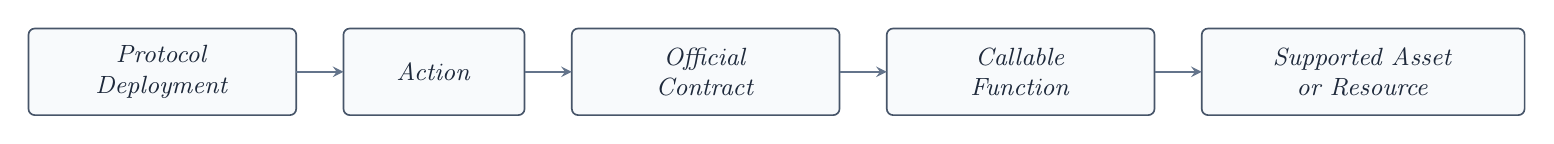
\begin{tikzpicture}[x=1cm,y=1cm,>=stealth]

% Colours
\definecolor{stepfill}{HTML}{F8FAFC}
\definecolor{stepborder}{HTML}{475569}
\definecolor{arrowcol}{HTML}{64748B}
\definecolor{steptext}{HTML}{1E293B}

% Protocol Deployment
\draw[rounded corners=0.08cm, draw=stepborder,
      fill=stepfill, line width=0.6pt]
  (0,0) rectangle (3.4,1.1);
\node[align=center, text=steptext, font=\small]
  at (1.7,0.55)
  {\textit{Protocol}\\\textit{Deployment}};

% Action
\draw[rounded corners=0.08cm, draw=stepborder,
      fill=stepfill, line width=0.6pt]
  (4.0,0) rectangle (6.3,1.1);
\node[align=center, text=steptext, font=\small]
  at (5.15,0.55)
  {\textit{Action}};

% Official Contract
\draw[rounded corners=0.08cm, draw=stepborder,
      fill=stepfill, line width=0.6pt]
  (6.9,0) rectangle (10.3,1.1);
\node[align=center, text=steptext, font=\small]
  at (8.6,0.55)
  {\textit{Official}\\\textit{Contract}};

% Callable Function
\draw[rounded corners=0.08cm, draw=stepborder,
      fill=stepfill, line width=0.6pt]
  (10.9,0) rectangle (14.3,1.1);
\node[align=center, text=steptext, font=\small]
  at (12.6,0.55)
  {\textit{Callable}\\\textit{Function}};

% Supported Asset or Resource
\draw[rounded corners=0.08cm, draw=stepborder,
      fill=stepfill, line width=0.6pt]
  (14.9,0) rectangle (19.0,1.1);
\node[align=center, text=steptext, font=\small]
  at (16.95,0.55)
  {\textit{Supported Asset}\\\textit{or Resource}};

% Arrows
\draw[->, line width=0.7pt, draw=arrowcol]
  (3.4,0.55) -- (4.0,0.55);

\draw[->, line width=0.7pt, draw=arrowcol]
  (6.3,0.55) -- (6.9,0.55);

\draw[->, line width=0.7pt, draw=arrowcol]
  (10.3,0.55) -- (10.9,0.55);

\draw[->, line width=0.7pt, draw=arrowcol]
  (14.3,0.55) -- (14.9,0.55);

\end{tikzpicture}%
}
\caption{Simplified action-oriented relationship path used for verification.}
\label{fig:action_oriented_relationship}
\end{figure}


The exact relationship depends on the requested action. A swap may additionally
require verification of a router, token pair, and corresponding liquidity pool.
A lending action may require verification of the protocol deployment, Pool
contract, lending function, and reserve asset. R2 does not prescribe a particular verification technology. Relationships may
be checked using structured rules, registries, policy engines, graph structures,
or another suitable mechanism.

\paragraph{Assessment criteria.}

R2 is assessed using the following criteria:

\begin{enumerate}
    \item[\textbf{C1}] The selected protocol deployment is checked against
    the requested action.

    \item[\textbf{C2}] The target contract and callable function are checked
    against the requested action.

    \item[\textbf{C3}] The required asset, pool, reserve, market, or other
    protocol-specific resource is checked against the selected action and
    deployment.

    \item[\textbf{C4}] The relationship validation is performed before
    blockchain execution.
\end{enumerate}


% \begin{table}[H]
% \centering
% \begin{tabular}{p{2.3cm} p{9.9cm}}
% \hline
% \textbf{Rating} & \textbf{Assessment Condition} \\ \hline

% $\star\star\star$ &
% All four criteria C1--C4 are supported. \\

% $\star\star\circ$ &
% Three criteria are supported, including C4. \\

% $\star\circ\circ$ &
% One or two criteria are supported, or three criteria are supported without
% pre-execution validation. \\

% $\circ\circ\circ$ &
% The approach does not validate the relationship between the requested action
% and the selected execution information. \\


% \hline
% \end{tabular}
% \caption{Assessment scale for R2: Intent-to-execution relationship validation}
% \label{tab:r2_scale}
% \end{table}
The general scale in Table~\ref{tab:general_assessment_scale} applies.
C4 is mandatory for a rating above $\star\circ\circ$ because R2 concerns
pre-execution validation rather than analysis of an already executed transaction.

% ============================================================
% R3
% ============================================================

\subsection{R3: Authoritative and Maintainable Verification Knowledge}
\label{subsec:r3_verification_knowledge}

\paragraph{Problem.}

The correctness of a verification decision depends on the information used as
the reference for that decision.

For example, checking whether a contract belongs to Aave V3 is useful only when
the expected contract information itself is trustworthy. An outdated contract
address, incorrect token mapping, wrong protocol version, or stale pool or
reserve relationship may lead to an incorrect verification result even when the
verification logic itself operates correctly. This problem is particularly relevant in DeFi because execution information may
differ between blockchain networks and protocol versions. Supported assets,
pools, reserves, and protocol deployments may also change over time. Verification knowledge must therefore have an identifiable origin and must be
maintainable when the supported environment changes.

\paragraph{Requirement.}

The system shall obtain verification information from identifiable trusted or
authoritative sources and shall retain sufficient context to determine where
the information originated and to which deployment it applies.

The system shall also allow outdated or changed verification information to be
updated or invalidated without redesigning the complete verification mechanism.

Relevant context may include:

\begin{itemize}
    \item the information source;
    \item blockchain network;
    \item protocol and protocol version;
    \item contract or asset address;
    \item synchronization or retrieval time; and
    \item validity or active status.
\end{itemize}

R3 does not require the use of a particular API or data-storage technology.
For example, a solution may obtain information from official protocol APIs,
deployment registries, verified on-chain data, protocol documentation, or
another identifiable authoritative source. R3 does not prescribe a particular information source,
synchronisation method, or data-storage technology.
The mechanisms selected to address this requirement
are discussed in the Concept and Implementation chapters.


\paragraph{Assessment criteria.}

R3 is assessed using the following criteria:

\begin{enumerate}
    \item[\textbf{C1}] Verification information originates from defined
    trusted or authoritative sources.

    \item[\textbf{C2}] The origin and relevant context of the verification
    information can be identified, including information such as source,
    network, or protocol version where applicable.

    \item[\textbf{C3}] Changed, outdated, or removed verification information
    can be updated or invalidated.

    \item[\textbf{C4}] Additional supported entities or relationships can be
    incorporated without redesigning the complete verification mechanism.
\end{enumerate}


The general scale in Table~\ref{tab:general_assessment_scale} applies.
C1 is mandatory for a rating above $\star\circ\circ$ because verification
knowledge must originate from an identifiable trusted or authoritative source.

For assessment, the accepted sources and the basis for treating them as
trusted or authoritative shall be stated explicitly. Source authority
shall be assessed for the relevant information and deployment context;
retrieval relevance or the presence of information in a knowledge base
alone does not establish authority.
% ============================================================
% R4
% ============================================================

\subsection{R4: Pre-Execution Enforcement and Controlled Execution}
\label{subsec:r4_enforcement}

\paragraph{Problem.}

Identifying an incorrect or unverifiable action does not protect the user if the
action can still proceed to signing or blockchain submission.

For example, a verification mechanism may correctly detect that the selected
contract does not belong to the requested protocol. If this result is presented
only as a warning while the transaction remains executable, the verification
mechanism does not provide an effective security boundary. A second problem occurs after an action has been approved. Approval of one
verified action should not provide an automated agent with unrestricted
authority over the user's wallet. The execution should remain limited to the
conditions that were verified.

\paragraph{Requirement.}

The system shall prevent rejected or unresolved actions from continuing toward
blockchain execution and shall allow approved actions to execute only under
defined execution restrictions.

The expected process is:

\begin{enumerate}
    \item the required verification checks are completed;
    \item an explicit approval or rejection is produced;
    \item rejected or unresolved actions are prevented from continuing;
    \item only approved actions are passed to the execution mechanism; and
    \item approved actions remain restricted to the verified execution
    conditions.
\end{enumerate}

Relevant restrictions may include permitted target contracts,
    permitted callable functions,
     transaction or spending limits,
    permitted recipients or spenders,
     blockchain-network restrictions,
    time-limited permissions and
    revocable delegated permissions. Programmable smart-account architectures can support such execution controls.
ERC-4337, for example, separates UserOperation validation from execution and
allows smart-account implementations to define their own validation logic
\cite{buterinERC4337AccountAbstraction2021,
linMeasurementInvestigationERC43372024}.

R4 does not require ERC-4337 specifically. The requirement concerns the
enforcement of the verification decision and controlled execution of an
approved action.

\paragraph{Assessment criteria.}

R4 is assessed using the following criteria:

\begin{enumerate}
    
\item[\textbf{C1}] An explicit verification outcome
is produced before blockchain execution, distinguishing
approval, rejection, and insufficient evidence.

\item[\textbf{C2}] Rejected or unresolved actions are
automatically prevented from continuing toward execution.


    \item[\textbf{C3}] Approved actions execute only within restrictions
that enforce the applicable verified execution conditions.

\item[\textbf{C4}] The executed operation remains bound to the approved
security-relevant parameters. Changes to these parameters require
revalidation of the modified operation before execution.
\end{enumerate}


The general scale in Table~\ref{tab:general_assessment_scale} applies.
C2 and C3 are mandatory for a rating above $\star\circ\circ$ because
the requirement covers enforcement of
negative decisions and controlling approved
execution.

% ============================================================
% R5
% ============================================================

\subsection{R5: Traceable Verification Result}
\label{subsec:r5_traceability}

\paragraph{Problem.}

A verification decision is difficult to inspect when the system returns only an
unexplained approval or rejection.

For example:

\begin{quote}
``Transaction rejected.''
\end{quote}

does not indicate whether the rejection was caused by the protocol, contract,
function, asset, amount, recipient, or another verification condition. This is particularly important when an AI-generated action appears reasonable
to the user but is rejected by the verification mechanism. The user, developer,
or evaluator should be able to identify which verification condition produced
the decision.

\paragraph{Requirement.}

The system shall provide a structured and traceable
verification result that identifies the outcome and
the conditions responsible for it. This includes
approval, rejection, and cases where sufficient
verification evidence is unavailable. The underlying result shall contain sufficient
information to identify the relevant verification
condition, entity, or relationship. Where applicable,
the expected and observed values shall be available
to support inspection of the decision.

For example, instead of returning only:

\begin{quote}
``Transaction rejected.''
\end{quote}

the system may report:

\begin{quote}
``Contract mismatch: the selected address does not match the expected contract
for the selected protocol deployment.''
\end{quote}

\paragraph{Assessment criteria.}

R5 is assessed using the following criteria:

\begin{enumerate}
    
\item[\textbf{C1}] The verification outcome,
including approval, rejection, or insufficient evidence,
is explicitly reported.

    \item[\textbf{C2}] A reason or stable verification identifier is
    provided.

    \item[\textbf{C3}] The specific field, rule, entity, or relationship
    responsible for the result can be identified.

    \item[\textbf{C4}] When a mismatch occurs, the expected and observed
    values are available when both values can be determined.
\end{enumerate}


% \begin{table}[H]
% \centering
% \begin{tabular}{p{2.3cm} p{9.9cm}}
% \hline
% \textbf{Rating} & \textbf{Assessment Condition} \\ \hline

% $\star\star\star$ &
% All four criteria C1--C4 are supported. \\

% $\star\star\circ$ &
% Three criteria are supported, including C3. \\

% $\star\circ\circ$ &
% One or two criteria are supported, or a general explanation is provided
% without identifying the exact verification condition. \\

% $\circ\circ\circ$ &
% The approach provides no usable explanation or traceable verification result. \\

% \hline
% \end{tabular}
% \caption{Assessment scale for R5: Traceable verification result}
% \label{tab:r5_scale}
% \end{table}

The general scale in Table~\ref{tab:general_assessment_scale} applies.
C3 is mandatory for a rating above $\star\circ\circ$ because a traceable
result must identify the verification condition responsible for the decision.
% ============================================================
% R6
% ============================================================

\subsection{R6: Bounded Verification Time}
\label{subsec:r6_latency}

\paragraph{Problem.}

The verification mechanism is positioned before blockchain execution and
therefore introduces an additional processing step into every protected
transaction.

Even if the verification decision is correct, an excessively slow verification
process may make the system unsuitable for interactive use. Terms such as
``fast'' or ``low latency'' are therefore insufficient unless the expected
processing time can be measured.

% \paragraph{Requirement.}

% A quantitative threshold is required so that the additional verification delay can be evaluated objectively. Since the verification stage is part of an interactive pre-execution workflow, this thesis adopts two seconds as a conservative prototype-specific upper bound for the verification decision.

% For the prototype developed in this thesis, the measurable target is
% defined:

% \begin{quote}
% At least 95\% of pre-execution verification decisions shall be returned within
% 2 seconds.
% \end{quote}

% The two-second threshold is a project-specific acceptance target for the prototype and is not presented as a universal performance requirement for all DeFi applications.

% The measurement begins when a complete structured intent reaches the
% verification stage and ends when the verification decision and its structured
% result are available. The measurement excludes, 
%     user input time,
%    LLM intent-generation time,
%     user wallet-confirmation time,
%     bundler processing time,
%      blockchain submission time, and
%     blockchain confirmation time of a transaction.

% These stages are excluded because R6 measures only the additional processing
% delay introduced by the verification mechanism. The two-second threshold is a project-specific acceptance target for the
% prototype and is not presented as a universal performance requirement for all
% DeFi applications. When existing approaches are assessed, a rating is assigned only when their
% reported measurements are sufficiently comparable with the defined
% pre-execution measurement boundary. Otherwise, the result is marked as
% \textit{N/E}.

\paragraph{Requirement.}

Pre-execution verification introduces additional processing
time into an interactive transaction workflow. To assess
this overhead, the thesis defines the following
prototype-specific acceptance target:

\begin{quote}
At least 95\% of pre-execution verification decisions
shall be returned within 2 seconds.
\end{quote}

The measurement begins when a complete structured intent
reaches the verification stage and ends when the structured
verification result becomes available. It excludes
natural-language processing, user interaction, wallet
confirmation, bundler processing, and blockchain submission
and confirmation times. The threshold is an evaluation target selected for this
prototype rather than a universal performance requirement.
Existing approaches are rated only when their reported
measurements are comparable with this measurement boundary.
Otherwise, the result is marked as \textit{N/E}.

\begin{table}[H]
\centering
\begin{tabular}{p{2.3cm} p{9.9cm}}
\hline
\textbf{Rating} & \textbf{Assessment Condition} \\ \hline

$\star\star\star$ &
At least 95\% of comparable pre-execution verification decisions complete
within 2 seconds. \\

$\star\star\circ$ &
At least 90\% but fewer than 95\% of comparable verification decisions complete
within 2 seconds. \\

$\star\circ\circ$ &
At least 75\% but fewer than 90\% of comparable verification decisions complete
within 2 seconds. \\

$\circ\circ\circ$ &
Fewer than 75\% of comparable verification decisions complete within
2 seconds, or the approach is explicitly designed only for offline or
post-execution analysis. \\


\hline
\end{tabular}
\caption{Assessment scale for R6: Bounded verification time}
\label{tab:r6_scale}
\end{table}


The following section reviews existing approaches and evaluates them against
these six requirements.

% ============================================================
% 2.2 Existing Approaches
% ============================================================

\section{Approaches}
\label{sec:sota_approaches}

% The requirements defined in Section~\ref{sec:requirements_analysis}
% describe the capabilities expected from a solution for secure
% AI-driven DeFi execution. This section reviews existing approaches
% that address different parts of these requirements. The literature
% is organised into five \textit{approach groups}, according to the
% main technical focus considered in the discussion:
% execution control, AI-assisted action generation, knowledge
% retrieval, graph-based relationship analysis, and smart-contract
% security analysis.

% These groups provide a structure for the review rather than a
% classification into mutually exclusive types of systems. They
% cover both technical mechanisms and analytical objectives.
% A single system may therefore contribute to more than one group.
% For example, a smart-contract security tool may use a graph to
% represent function calls or data dependencies. Its graph
% representation is relevant to graph-based relationship analysis,
% while its investigation of vulnerabilities is relevant to
% smart-contract security analysis. The distinction between these two groups concerns the aspect
% being examined. Graph-based relationship analysis focuses on
% how connected information is represented, queried, or analysed.
% Smart-contract security analysis focuses on whether contract
% code or behaviour exhibits vulnerabilities or violates specified
% properties. Their overlap does not make them interchangeable.
% Where a system is discussed in both groups, each discussion
% addresses the aspect relevant to that group.

% Individual standards, frameworks, and research systems are
% examined as representative examples. For each group, the review
% considers the information processed, the mechanism applied,
% the result produced, and its relevance to the requirements.
% It distinguishes capabilities demonstrated by the reviewed
% systems from capabilities that depend on additional components.
% A practical solution may combine several groups, such as
% AI-assisted intent generation, relationship verification,
% and execution controls.

% Table~\ref{tab:approach_groups} summarises the focus of each group.
% The requirement comparison in Section~\ref{sec:sota_comparison}
% assesses their coverage of R1--R6. Similar ratings indicate
% similar coverage under the assessment criteria; they do not
% imply that the approaches have the same purpose or are
% technically equivalent.


The requirements defined in Section~\ref{sec:requirements_analysis}
describe the capabilities expected from a solution for secure
AI-driven DeFi execution. This section reviews existing approaches
that address different parts of these requirements. The literature
is organised into five \textit{approach groups} according to their
primary technical focus: execution control, AI-assisted blockchain
action generation, knowledge retrieval, graph-based relationship
analysis, and smart-contract security analysis.

Each approach group represents a broad technical direction. Within
these groups, subgroups distinguish methods according to their
underlying mechanisms or analytical objectives. Individual
standards, frameworks, and research systems are discussed as
representative examples of the corresponding methods. This
distinction is important because the capabilities demonstrated by
one system do not necessarily apply to every approach within
the same group.

The groups are not mutually exclusive. A system may combine
mechanisms from several groups or be relevant to more than
one analytical objective. For example, smart-contract security
analysis may use graphs to represent function calls or data
dependencies. Such representations are relevant to graph-based
relationship analysis, while the identification of vulnerabilities
belongs to smart-contract security analysis. The distinction
therefore concerns the purpose for which a mechanism is used,
rather than the presence of a particular technology. For each group, the review first considers its general
characteristics, including the information processed, the
mechanisms applied, and the results produced. The subsequent
discussion examines the relevant subgroups and representative
systems, including their contributions and limitations with
respect to the requirements. Capabilities inherent to a method
are distinguished from those demonstrated by individual
implementations or requiring additional components.

Figure~\ref{fig:approach_hierarchy} provides an overview of
the reviewed approach groups and their subgroups.
Table~\ref{tab:approach_groups} summarises the technical focus
of each group. The requirement
comparison in Section~\ref{sec:sota_comparison} assesses their
coverage of R1 to R6. Similar ratings indicate similar coverage
under the assessment criteria; they do not imply that the
approaches have the same purpose or are technically equivalent.



\begin{table}[H]
\centering
\small
\renewcommand{\arraystretch}{1.15}
\begin{tabular}{p{4.8cm} p{9.2cm}}
\hline
\textbf{Approach Group} & \textbf{Focus of the Review} \\
\hline

Execution-Layer Security and Policy Enforcement &
Mechanisms that authorise or block prepared operations and
restrict the execution authority available to an account
or automated agent. \\

AI-Agent Blockchain Execution &
Methods that translate natural-language goals into structured
actions, tool calls, workflows, and blockchain operations. \\

Knowledge Retrieval and Grounding &
Methods that obtain external information to support
interpretation, planning, analysis, or verification. \\

Graph-Based Relationship Analysis &
Methods that represent and examine connected information,
including transaction flows, program dependencies, domain
knowledge, and validation dependencies. \\

Smart Contract Security Analysis &
Methods that examine contract code, execution behaviour,
and cross-contract interactions for vulnerabilities or
violations of specified properties. \\

\hline
\end{tabular}
\caption{Technical focus of the five approach groups reviewed.}
\label{tab:approach_groups}
\end{table}

\begin{figure}[H]
\centering
\begingroup

\definecolor{stepfill}{HTML}{F8FAFC}
\definecolor{stepborder}{HTML}{475569}
\definecolor{arrowcol}{HTML}{64748B}
\definecolor{steptext}{HTML}{1E293B}

\resizebox{0.98\linewidth}{!}{%
\begin{tikzpicture}[
    x=1cm, y=1cm,
    root/.style={
        draw=stepborder,
        fill=stepfill,
        rounded corners=2pt,
        line width=0.75pt,
        text=steptext,
        text width=5cm,
        minimum height=0.83cm,
        align=center,
        inner sep=5pt,
        font=\sffamily\bfseries
             \fontsize{10}{12}\selectfont
    },
    group/.style={
        draw=stepborder,
        fill=stepfill,
        rounded corners=2pt,
        line width=0.65pt,
        text=steptext,
        text width=3.95cm,
        minimum height=1.12cm,
        align=center,
        inner sep=5pt,
        font=\sffamily\bfseries
             \fontsize{10}{12}\selectfont
    },
    subgroup/.style={
        draw=stepborder,
        fill=white,
        rounded corners=2pt,
        line width=0.5pt,
        text=steptext,
        text width=3.75cm,
        minimum height=1.08cm,
        align=center,
        inner xsep=5pt,
        inner ysep=5pt,
        font=\sffamily
             \fontsize{10}{12}\selectfont
    },
    synthesis/.style={
        subgroup,
        dashed
    },
    link/.style={
        draw=arrowcol,
        line width=0.65pt
    }
]

% =====================================================
% LEVEL 1: ROOT
% =====================================================

\node[root] (root) at (0,0)
    {Existing Approaches};


% =====================================================
% LEVEL 2: FIVE APPROACH GROUPS
% =====================================================

\node[group] (g1) at (-9.8,-1.95)
    {Execution-Layer Security\\
     and Policy Enforcement};

\node[group] (g2) at (-4.9,-1.95)
    {AI-Agent Blockchain\\
     Execution};

\node[group] (g3) at (0,-1.95)
    {Knowledge Retrieval\\
     and Grounding};

\node[group] (g4) at (4.9,-1.95)
    {Graph-Based Relationship\\
     Analysis};

\node[group] (g5) at (9.8,-1.95)
    {Smart Contract\\
     Security Analysis};


% =====================================================
% ROOT-TO-GROUP BRANCHES
% =====================================================

\draw[link]
    (root.south) -- (0,-0.85);

\draw[link]
    (-9.8,-0.85) -- (9.8,-0.85);

\foreach \n in {1,2,3,4,5} {
    \draw[link]
        (g\n.north) --
        (g\n.north |- 0,-0.85);
}


% =====================================================
% LEVEL 3: GROUP 1
% Execution-Layer Security and Policy Enforcement
% =====================================================

\node[subgroup] (a1) at (-9.65,-4.05)
    {ERC-4337 and\\
     programmable smart accounts};

\node[subgroup] (a2) at (-9.65,-5.60)
    {Transaction simulation};


% =====================================================
% LEVEL 3: GROUP 2
% AI-Agent Blockchain Execution
% =====================================================

% Individual systems are representative examples.

\node[subgroup] (b1) at (-4.75,-4.05)
    {Tool-based action frameworks\\
     \textit{Coinbase AgentKit}};

\node[subgroup] (b2) at (-4.75,-5.60)
    {Workflow-grounded agents\\
     \textit{Web3Agent}};

\node[subgroup] (b3) at (-4.75,-7.15)
    {Intent-to-transaction verification\\
     \textit{Arbiter}};

\node[subgroup] (b4) at (-4.75,-8.70)
    {Transaction-intent mining\\
     \textit{Related research}};


% =====================================================
% LEVEL 3: GROUP 3
% Knowledge Retrieval and Grounding
% =====================================================

\node[subgroup] (c1) at (0.15,-4.05)
    {Retrieval-grounded blockchain\\
     and security systems};

\node[subgroup] (c2) at (0.15,-5.60)
    {GraphRAG and\\
     graph-assisted retrieval};


% =====================================================
% LEVEL 3: GROUP 4
% Graph-Based Relationship Analysis
% =====================================================

\node[subgroup] (d1) at (5.05,-4.05)
    {Transaction and\\
     cash-flow graphs};

\node[subgroup] (d2) at (5.05,-5.60)
    {Code and cross-contract graphs};

\node[subgroup] (d3) at (5.05,-7.15)
    {Knowledge graphs and\\
     semantic relationship models};

\node[subgroup] (d4) at (5.05,-8.70)
    {Validation-workflow graphs};

% The final box represents a synthesis, not
% a separate approach subgroup.

\node[synthesis] (d5) at (5.05,-10.25)
    {Relevance of property graphs\\
     to verification (synthesis)};


% =====================================================
% LEVEL 3: GROUP 5
% Smart Contract Security Analysis
% =====================================================

\node[subgroup] (e1) at (9.95,-4.05)
    {Static, symbolic, and\\
     formal analysis};

\node[subgroup] (e2) at (9.95,-5.60)
    {LLM-assisted smart\\
     contract auditing};

\node[subgroup] (e3) at (9.95,-7.15)
    {Cross-contract and\\
     DeFi-specific analysis};


% =====================================================
% CONNECTIONS: GROUP 1
% =====================================================

\draw[link]
    (g1.south) -- (-9.8,-3.10)
    -- (-12.0,-3.10)
    -- (-12.0,-5.60);

\draw[link]
    (-12.0,-4.05) -- (a1.west);

\draw[link]
    (-12.0,-5.60) -- (a2.west);


% =====================================================
% CONNECTIONS: GROUP 2
% =====================================================

\draw[link]
    (g2.south) -- (-4.9,-3.10)
    -- (-7.1,-3.10)
    -- (-7.1,-8.70);

\draw[link]
    (-7.1,-4.05) -- (b1.west);

\draw[link]
    (-7.1,-5.60) -- (b2.west);

\draw[link]
    (-7.1,-7.15) -- (b3.west);

\draw[link]
    (-7.1,-8.70) -- (b4.west);


% =====================================================
% CONNECTIONS: GROUP 3
% =====================================================

\draw[link]
    (g3.south) -- (0,-3.10)
    -- (-2.2,-3.10)
    -- (-2.2,-5.60);

\draw[link]
    (-2.2,-4.05) -- (c1.west);

\draw[link]
    (-2.2,-5.60) -- (c2.west);


% =====================================================
% CONNECTIONS: GROUP 4
% =====================================================

\draw[link]
    (g4.south) -- (4.9,-3.10)
    -- (2.7,-3.10)
    -- (2.7,-10.25);

\draw[link]
    (2.7,-4.05) -- (d1.west);

\draw[link]
    (2.7,-5.60) -- (d2.west);

\draw[link]
    (2.7,-7.15) -- (d3.west);

\draw[link]
    (2.7,-8.70) -- (d4.west);

\draw[link]
    (2.7,-10.25) -- (d5.west);


% =====================================================
% CONNECTIONS: GROUP 5
% =====================================================

\draw[link]
    (g5.south) -- (9.8,-3.10)
    -- (7.6,-3.10)
    -- (7.6,-7.15);

\draw[link]
    (7.6,-4.05) -- (e1.west);

\draw[link]
    (7.6,-5.60) -- (e2.west);

\draw[link]
    (7.6,-7.15) -- (e3.west);


\end{tikzpicture}%
}

\endgroup

\caption{Hierarchy of the five approach groups
and the subtopics reviewed.}

\label{fig:approach_hierarchy}

\end{figure}


% ============================================================
% 2.2.1
% ============================================================

% \subsection{Execution-Layer Security and Policy Enforcement Approaches}
% \label{subsec:execution_layer_security}

% Execution-layer security approaches operate near the point where a blockchain
% operation is authorised, signed, or submitted. Their input is normally an
% already prepared transaction, wallet request, or smart-account operation.
% Their main purpose is to determine whether the operation is permitted under a
% defined execution policy. These policies may restrict elements such as the target contract, callable
% function, recipient, amount, blockchain network, execution period, or authority
% granted to an automated agent. If a policy condition fails, the operation can
% be rejected before blockchain execution.

% This capability is especially relevant to R4 because detecting an incorrect
% action is useful only when the verification result can prevent execution.
% Execution-layer security also provides a mechanism for limiting the authority
% of approved automated actions. However, execution policy and intent correctness are different concerns. A
% transaction can satisfy a wallet policy while still representing the wrong
% interpretation of the user's request. For example, an agent may be permitted to
% interact with an official protocol contract, but the selected function or asset
% may still not correspond to the requested operation.

% Execution-layer controls therefore provide a strong enforcement boundary, but
% they generally depend on another component to determine what should be accepted
% or rejected.


% \subsubsection{ERC-4337 and Programmable Smart Accounts}

% ERC-4337 introduces an account-abstraction architecture in which users submit
% \textit{UserOperations} that are processed through an EntryPoint contract
% \cite{buterinERC4337AccountAbstraction2021,
% linMeasurementInvestigationERC43372024}. A smart account validates a UserOperation according to its programmed account
% logic before execution. This enables more flexible authorisation than the
% traditional Externally Owned Account (EOA) model.

% The architecture is relevant to automated agents because account validation can
% support application-specific authorization rules. However, ERC-4337 itself does
% not define whether a particular Aave supply operation, Uniswap swap, token
% approval, or transfer correctly represents a natural-language request. It therefore provides infrastructure through which a verification decision can
% be enforced rather than providing the complete intent-verification mechanism
% itself.

% Modular smart-account architectures extend this idea. ERC-7579 defines
% interfaces for modular smart accounts and account modules
% \cite{erc7579MinimalModularSmartAccounts2023}. Such modularity allows
% additional validation and execution logic to be introduced without placing all
% security functionality directly inside the core account. ZeroDev documents delegated permissions and session-key mechanisms that can
% limit what an automated process is allowed to perform
% \cite{zeroDevPermissionsSessionKeys2026}. Safe Guards similarly allow
% transaction parameters to be inspected and can reject a transaction when the
% defined guard conditions are not satisfied
% \cite{safeSmartAccountGuards2026}. Safe also documents smart-account
% architectures for AI-agent interaction
% \cite{safeAIAgentsSmartAccounts2026}.

% These mechanisms strongly contribute to R4 by supporting mandatory blocking and
% controlled execution. Their contribution to R2 and R3 depends on the
% verification rules and knowledge supplied to them. A smart account does not
% automatically maintain an authoritative model of DeFi protocol relationships.


% \subsubsection{Transaction Simulation}

% Transaction simulation evaluates a candidate transaction against a selected
% blockchain state without committing its resulting state changes. Tenderly, for example, provides simulation results such as execution status,
% contract calls, emitted events, state changes, and asset changes
% \cite{tenderlyTransactionSimulation2026}. Simulation is useful because it can identify a transaction that would revert or
% produce unexpected state changes before the transaction is submitted. However, simulation normally begins after the target contract and calldata have
% already been selected.\\ It therefore primarily answers:

% \begin{quote}
% ``What is this prepared transaction expected to do?''
% \end{quote}

% The verification problem considered in this thesis asks an earlier question:

% \begin{quote}
% ``Does this execution information correctly represent the user's requested
% action?''
% \end{quote}

% A transaction may simulate successfully while targeting an unintended but
% technically valid contract or function. Simulation can therefore provide
% additional evidence for R2, but it does not independently establish the
% complete intent-to-execution relationship.

% \paragraph{Relationship to the requirements.}

% Execution-layer approaches primarily address R4 because smart accounts,
% guards, and permission mechanisms can block rejected operations and restrict
% approved execution. They provide limited support for R2 and R3 when trusted
% contracts or execution policies are configured externally, and they can
% contribute to R5 through identifiable policy failures. They do not normally
% generate structured intents, while comparable evidence for R6 is insufficient.


% \begin{table}[H]
% \centering
% \renewcommand{\arraystretch}{1.3}
% \begin{tabular}{cccccc}
% \hline
% \textbf{R1} & \textbf{R2} & \textbf{R3} & \textbf{R4} & \textbf{R5} & \textbf{R6} \\ \hline

% $\circ\circ\circ$ &
% $\star\circ\circ$ &
% $\star\circ\circ$ &
% $\star\star\star$ &
% $\star\star\circ$ &
% \textit{N/E} \\

% \hline
% \end{tabular}
% \caption{Requirement coverage of execution-layer security and policy enforcement approaches}
% \label{tab:req_execution_layer}
% \end{table}


\subsection{Execution-Layer Security and Policy Enforcement Approaches}
\label{subsec:execution_layer_security}

Execution-layer security approaches control whether a prepared
blockchain operation is authorised to proceed toward execution.
They typically operate after an action has been translated into
transaction parameters, a wallet request, or a smart-account
operation. Their primary concern is not the interpretation of
the user's original request, but whether the resulting operation
satisfies defined authorisation and execution conditions.

A central characteristic of this group is the enforcement of
restrictions on the authority available to an account or
automated agent. Such restrictions may concern the target
contract, callable function, recipient, token, amount, network,
or period during which an operation is permitted. Programmable
smart accounts support application-specific validation, while
modular account architectures allow additional authorisation
and execution mechanisms to be incorporated
\cite{buterinERC4337AccountAbstraction2021,
erc7579MinimalModularSmartAccounts2023}.
Permission mechanisms and transaction guards provide further
means of restricting automated operations
\cite{zeroDevPermissionsSessionKeys2026,
safeSmartAccountGuards2026}.

The result of an execution policy check is generally a decision
to permit or prevent an operation under the configured
conditions. Transaction simulation provides a related but
different form of pre-execution assessment. It examines the
expected behaviour of a prepared transaction and can reveal
execution failures or unexpected state changes without
submitting the transaction to the blockchain
\cite{tenderlyTransactionSimulation2026}. Simulation findings
can inform an execution decision, but they do not automatically
enforce one. These approaches are particularly relevant to AI-driven DeFi
because an automated agent may generate technically valid
operations that exceed its intended authority. Execution-layer
controls can restrict such operations independently of the
component that generated them. However, satisfying an execution
policy does not establish that the selected action correctly
represents the user's request. An agent may be authorised to
interact with an official protocol contract while selecting an
unintended function or asset. Execution control therefore
depends on separately defined rules or verification results
when intent correctness must also be established.

Two technical directions are considered within this group:
programmable smart accounts and policy controls, which restrict
execution authority, and transaction simulation, which examines
the expected effects of prepared operations.

\subsubsection{ERC-4337 and Programmable Smart Accounts}

Programmable smart accounts allow authorisation conditions to
be defined through account logic rather than relying only on
the signature-based authorisation of an Externally Owned
Account (EOA). This supports mechanisms such as delegated
permissions, restricted operations, and application-specific
validation rules. ERC-4337 introduces an account-abstraction architecture based
on \textit{UserOperations}, an EntryPoint contract, and
smart-account validation
\cite{buterinERC4337AccountAbstraction2021,
linMeasurementInvestigationERC43372024}.
A smart account validates a UserOperation according to its
implemented logic before execution. ERC-7579 extends the
design possibilities by specifying interfaces for modular
smart accounts and their validation and execution modules
\cite{erc7579MinimalModularSmartAccounts2023}.

Individual implementations demonstrate different policy
mechanisms. ZeroDev documents delegated permissions and
session keys that can restrict an automated process to
specified operations
\cite{zeroDevPermissionsSessionKeys2026}.
Safe Guards can inspect transaction parameters and prevent
execution when configured conditions are violated
\cite{safeSmartAccountGuards2026}.
Safe also describes smart-account applications involving
AI agents \cite{safeAIAgentsSmartAccounts2026}.

These mechanisms demonstrate how authorisation and execution
restrictions can be enforced, although the available controls
depend on the account implementation and its configuration.
Neither ERC-4337 nor programmable account logic inherently
determines whether a particular DeFi operation correctly
represents a natural-language intent. This requires additional
verification rules and reference information. Smart-account
mechanisms can enforce such a decision once it has been
established.

\subsubsection{Transaction Simulation}

Transaction simulation examines the expected execution of
a prepared blockchain transaction against a selected
blockchain state without committing its resulting changes.
It typically receives transaction parameters and calldata
and produces information about execution status, contract
calls, state changes, events, or asset movements. Tenderly provides a representative implementation, including
transaction traces, execution results, and state and asset
changes \cite{tenderlyTransactionSimulation2026}.
These results can help identify transactions that would
revert or behave unexpectedly before submission.

Simulation primarily answers the question:

\begin{quote}
``What is this prepared transaction expected to do?''
\end{quote}

The verification problem considered in this thesis asks:

\begin{quote}
``Does this execution information correctly represent the
user's requested action?''
\end{quote}

A transaction may simulate successfully while calling an
unintended but technically valid contract or function.
Simulation therefore provides useful behavioural evidence
but does not independently establish the correctness of
the intent-to-execution relationship. Preventing submission
based on simulation findings also requires an additional
enforcement mechanism.

\paragraph{Relationship to the requirements.}


Execution-layer security and policy enforcement approaches
primarily address R4 by restricting execution authority and
blocking operations that violate configured policies
\cite{buterinERC4337AccountAbstraction2021,
zeroDevPermissionsSessionKeys2026,
safeSmartAccountGuards2026}. Binding execution to verified
parameters depends on the implemented controls. Their contribution to R2 is limited to checking selected
transaction parameters, such as contracts, functions, or
recipients, without inherently validating the complete
intent-to-execution relationship. Similarly, R3 receives
limited support because authoritative knowledge acquisition
and maintenance are not intrinsic to these mechanisms.

These approaches can support R5 through identifiable policy
failures and simulation results, including transaction traces
\cite{safeSmartAccountGuards2026,
tenderlyTransactionSimulation2026}. However, the available
decision evidence depends on the implementation. They do
not inherently provide natural-language intent generation
under R1, while comparable verification-time measurements
for R6 are not established by the reviewed evidence.

\begin{table}[H]
\centering
\renewcommand{\arraystretch}{1.3}
\begin{tabular}{cccccc}
\hline
\textbf{R1} & \textbf{R2} & \textbf{R3} &
\textbf{R4} & \textbf{R5} & \textbf{R6} \\
\hline

$\circ\circ\circ$ &
$\star\circ\circ$ &
$\star\circ\circ$ &
$\star\star\star$ &
$\star\star\circ$ &
\textit{N/E} \\

\hline
\end{tabular}
\caption{Requirement coverage of execution-layer security
and policy enforcement approaches}
\label{tab:req_execution_layer}
\end{table}

% ============================================================
% 2.2.2
% ============================================================

% \subsection{AI-Agent Blockchain Execution Approaches}
% \label{subsec:ai_agent_blockchain_execution}

% AI-agent blockchain execution approaches connect natural-language reasoning
% with blockchain functionality. A user describes a desired action, and a
% Large Language Model (LLM) selects an available tool, workflow, or action and
% generates the required parameters. The output may be a structured tool call, a multi-step execution plan,
% transaction parameters, or a candidate blockchain operation.

% The main strength of this category is its ability to convert a human-readable
% request into a structured representation that software can process. It is
% therefore closely related to R1. Tool-based architectures also reduce the execution space available to an LLM.
% Instead of generating arbitrary blockchain interactions, an agent selects from
% predefined actions with structured input schemas.

% However, structured output does not guarantee correct output. The model may
% select a valid action while choosing the wrong protocol, network, token,
% recipient, spender, amount, or other parameter. This creates an important distinction between \textit{action generation} and
% \textit{action verification}. AI-agent frameworks primarily help determine
% what action should be constructed. Additional verification is needed when the
% selected action must be checked against authoritative execution information.


% \subsubsection{Coinbase AgentKit}

% Coinbase AgentKit provides a practical architecture for connecting AI agents
% with blockchain functionality through wallet providers and action providers
% \cite{coinbaseAgentKit2026}. Action providers expose structured blockchain operations to the agent. The
% agent selects an action and supplies parameters, while application code handles
% the underlying blockchain interaction. This structure contributes to R1 because actions are exposed through defined
% schemas rather than unrestricted natural-language output. It can also reduce
% the set of operations available to an agent.

% However, the existence of an action provider does not by itself establish an
% independent verification layer. Protocol knowledge may be encoded inside the
% action provider or application code, but the framework does not inherently
% maintain a reusable model that checks the complete relationship between the
% user intent, protocol deployment, contract, function, and asset before
% execution. AgentKit is therefore primarily an execution-enablement framework. Verification
% and execution restrictions depend on the additional components with which it is
% combined.


% \subsubsection{Web3Agent}

% Web3Agent provides natural-language-driven blockchain interaction together with
% retrieved workflow, API, and error-handling knowledge
% \cite{TODO_Web3Agent}. A relevant contribution of Web3Agent is that it does not simply generate a
% transaction and execute it. It evaluates workflow consistency and contextual
% feasibility before execution. This makes Web3Agent relevant to both R1 and R2. It demonstrates that
% pre-execution reasoning about blockchain workflows already exists.

% However, workflow feasibility is not identical to validating an authoritative
% protocol execution relationship. A workflow may be logically feasible while
% still depending on an outdated deployment address, an incorrect network, an
% unsupported reserve, or another execution relationship that requires
% authoritative protocol information. Web3Agent can therefore contribute to R2 and R3 when the retrieved information
% has identifiable authority, version, and update properties. Its exact coverage
% depends on the information sources and verification rules demonstrated by the
% system.


% \subsubsection{Arbiter}

% Arbiter is one of the closest existing approaches to the verification problem
% considered in this thesis. It receives a natural-language intent together with
% a proposed DeFi transaction and evaluates whether the transaction is aligned
% with that intent \cite{TODO_Arbiter2026}. The approach combines technical validation with LLM-supported semantic checks.
% Its reported checks include canonical-address validation, amounts and decimals,
% slippage, fees, deadlines, parameter manipulation, and broader
% intent-transaction inconsistencies. Arbiter can produce an auditable \textit{ACCEPT} or \textit{REJECT} result
% before execution. It therefore directly demonstrates that pre-execution
% intent-transaction verification is possible and substantially contributes to
% R2, R4, and R5.

% Arbiter also uses a Graph-of-Thoughts structure. However, the meaning of its
% graph differs from the property graph investigated in this thesis. Arbiter's
% graph represents dependencies between validation operations. The graph proposed
% in this thesis represents persistent DeFi domain knowledge, including protocol
% deployments, actions, official contracts, functions, assets, pools, and
% reserves. The distinction is therefore not whether pre-execution verification exists, but
% how the verification knowledge is represented, maintained, queried, and
% connected to wallet execution.


% \subsubsection{Transaction Intent Mining}

% Transaction-intent mining approaches attempt to infer the likely purpose or
% semantic meaning of blockchain transactions
% \cite{TODO_TransactionIntentMining}. These approaches can support transaction classification, monitoring, forensic
% analysis, and behavioural understanding. However, their typical workflow begins
% with an observed or historical blockchain transaction.

% They therefore answer a question such as:

% \begin{quote}
% ``What was the likely purpose of this transaction?''
% \end{quote}

% rather than:

% \begin{quote}
% ``Should this proposed transaction be allowed to execute for the current user
% request?''
% \end{quote}

% They are relevant to semantic understanding but are not direct replacements for
% pre-execution validation and enforcement.

% \paragraph{Relationship to the requirements.}

% AI-agent blockchain execution approaches provide strong support for R1 by
% transforming natural-language requests into structured blockchain actions.
% Systems such as Web3Agent and Arbiter additionally provide pre-execution checks
% related to R2 and traceable results related to R5. Their support for trusted
% knowledge management and mandatory wallet enforcement is more limited and
% usually depends on additional components.
% \begin{table}[H]
% \centering
% \renewcommand{\arraystretch}{1.3}
% \begin{tabular}{cccccc}
% \hline
% \textbf{R1} & \textbf{R2} & \textbf{R3} & \textbf{R4} & \textbf{R5} & \textbf{R6} \\ \hline

% $\star\star\circ$ &
% $\star\star\circ$ &
% $\star\circ\circ$ &
% $\star\circ\circ$ &
% $\star\star\circ$ &
% \textit{N/E} \\

% \hline
% \end{tabular}
% \caption{Requirement coverage of AI-agent blockchain execution approaches}
% \label{tab:req_ai_agent}
% \end{table}


\subsection{AI-Agent Blockchain Execution Approaches}
\label{subsec:ai_agent_blockchain_execution}

AI-agent blockchain execution approaches connect natural-language
interaction with blockchain operations. Their primary purpose is
to transform a user's request into a structured action that can
be processed by blockchain software. Depending on the approach,
the generated result may be a tool call, an execution plan,
transaction parameters, or a candidate blockchain operation.
Frameworks such as Coinbase AgentKit demonstrate how predefined
blockchain actions can be exposed to AI agents, while systems
such as Web3Agent incorporate workflow information into
blockchain interaction
\cite{coinbaseAgentKit2026,TODO_Web3Agent}.

A central characteristic of this group is the separation
between language-based action selection and the technical
operations performed by blockchain tools. Rather than allowing
an LLM to interact directly with arbitrary contracts, an
application may expose predefined actions with structured
input parameters. This constrains the available operations
and allows application code to handle transaction construction
and blockchain communication
\cite{coinbaseAgentKit2026}. Other approaches extend this
process by incorporating workflow reasoning or additional
checks before execution
\cite{TODO_Web3Agent,TODO_Arbiter2026}. The main contribution of these approaches is the conversion
of human-readable instructions into machine-readable blockchain
actions. This is particularly relevant to R1 because DeFi
operations require explicit parameters such as the action,
protocol, asset, amount, and recipient. However, producing
a structurally valid action does not establish that its
parameters correctly represent the user's intention.
An agent may select an available tool while providing an
incorrect network, contract, asset, or other execution
parameter. The distinction between action generation and
action verification is therefore important.

The reviewed literature covers several related technical
directions: tool-based blockchain action generation,
workflow-grounded agents, and intent-to-transaction
verification. Transaction-intent mining is also considered
as related research on the interpretation of blockchain
operations. These directions differ in their inputs,
mechanisms, and objectives, although they all contribute
to understanding the relationship between human intentions
and blockchain transactions.

\subsubsection{Tool-Based Blockchain Action Generation}

Tool-based approaches expose blockchain functionality through
predefined operations with structured parameters. The agent
selects an available operation and supplies the required
information, while application code performs the underlying
blockchain interaction. This reduces the need for the LLM
to generate unrestricted transaction logic. 

Coinbase AgentKit is a representative framework that provides
wallet providers and action providers for blockchain
interaction \cite{coinbaseAgentKit2026}. Action providers
define operations that an agent can invoke through structured
interfaces. The framework therefore supports the generation
of machine-readable blockchain actions and restricts the
operations exposed to the model. However, the availability of a structured action does not
independently establish that the selected protocol, contract,
function, and asset correspond to the user's request.
Verification may be implemented within an action provider
or through additional application components, but a
separate authoritative relationship-verification mechanism
is not inherent to the framework.

\subsubsection{Workflow-Grounded Blockchain Agents}

Workflow-grounded approaches extend action generation by
incorporating information about the steps, dependencies,
and conditions required to perform blockchain operations.
This allows the agent to consider whether a proposed
sequence of actions is feasible rather than selecting
individual tools without contextual information. 

Web3Agent represents this direction by combining
natural-language blockchain interaction with retrieved
workflow, API, and error-handling knowledge
\cite{TODO_Web3Agent}. Its workflow consistency and
contextual feasibility checks provide a form of
pre-execution assessment beyond structured action
generation alone. Nevertheless, workflow feasibility does not necessarily
establish that the underlying execution information is
authoritative or current. An operation may follow a
feasible workflow while relying on an outdated deployment,
incorrect network, or unsupported protocol resource.
Its contribution to authoritative verification therefore
depends on the reliability, applicability, and maintenance
of the information used.

\subsubsection{Intent-to-Transaction Verification}

Intent-to-transaction verification approaches examine whether
a proposed blockchain transaction is consistent with the
user's expressed objective. Unlike approaches primarily
concerned with generating actions, their main purpose is
to identify inconsistencies before execution.

Arbiter is a particularly relevant representative because
it compares a natural-language DeFi intent with a proposed
transaction \cite{TODO_Arbiter2026}. It combines technical
validation with LLM-supported semantic checks, including
canonical addresses, amounts, token decimals, slippage,
fees, deadlines, and potential parameter manipulation.
The system produces an auditable \textit{ACCEPT} or
\textit{REJECT} decision before execution. Arbiter also employs a Graph-of-Thoughts structure to
organise dependencies between validation operations.
This differs from a persistent property graph containing
protocol deployments, contracts, functions, assets,
pools, and reserves. Its graph structures the verification
procedure rather than maintaining the domain relationships
against which an execution path is checked. Arbiter demonstrates that pre-execution verification of
DeFi transactions against user intentions is already
being investigated. The relevant distinction for this
thesis is therefore not the existence of such verification,
but the representation and maintenance of authoritative
execution relationships and their use in deterministic
verification decisions.

\subsubsection{Transaction-Intent Mining}

Transaction-intent mining is a related research direction
that attempts to infer the purpose or semantic meaning
of blockchain transactions
\cite{TODO_TransactionIntentMining}. These approaches
typically examine observed transactions or historical
blockchain activity and may support classification,
monitoring, or forensic analysis. Their primary objective differs from pre-execution
verification. Transaction-intent mining generally asks
what an observed transaction was intended to accomplish,
whereas the problem considered in this thesis concerns
whether a proposed transaction should be accepted for
the current user request.

These approaches contribute to the understanding of
transaction semantics but do not inherently provide
authoritative pre-execution validation or execution
enforcement.

\paragraph{Relationship to the requirements.}

AI-agent blockchain execution approaches primarily support
R1 by transforming natural-language requests into structured
blockchain actions. Tool-based frameworks provide defined
action interfaces, while workflow-grounded agents incorporate
execution context \cite{coinbaseAgentKit2026,TODO_Web3Agent}.
However, detecting incomplete or ambiguous parameters is
not a general capability of the group. Individual approaches also contribute to R2. Web3Agent
examines workflow consistency and contextual feasibility,
while Arbiter performs pre-execution checks of transaction
consistency with user intent
\cite{TODO_Web3Agent,TODO_Arbiter2026}.
These mechanisms address aspects of intent validation but
do not, as a group, demonstrate systematic verification of
all action-specific execution relationships defined by R2.

Support for R3 depends on the authority, provenance, and
maintenance of external information. Similarly, R4 requires
enforcement mechanisms beyond producing a verification
decision. For R5, Arbiter demonstrates traceable validation
through identifiable checks and decision evidence
\cite{TODO_Arbiter2026}, although this capability is not
inherent to all AI-agent frameworks. For R6, the reviewed
results do not establish sufficiently comparable measurements
within the verification-time boundary defined in this thesis.

\begin{table}[H]
\centering
\renewcommand{\arraystretch}{1.3}
\begin{tabular}{cccccc}
\hline
\textbf{R1} & \textbf{R2} & \textbf{R3} &
\textbf{R4} & \textbf{R5} & \textbf{R6} \\
\hline

$\star\star\circ$ &
$\star\star\circ$ &
$\star\circ\circ$ &
$\star\circ\circ$ &
$\star\star\circ$ &
\textit{N/E} \\

\hline
\end{tabular}
\caption{Requirement coverage of AI-agent blockchain
execution approaches}
\label{tab:req_ai_agent}
\end{table}

% ============================================================
% 2.2.3
% ============================================================

% \subsection{Knowledge Retrieval and Grounding Approaches}
% \label{subsec:knowledge_retrieval_grounding}

% Knowledge retrieval and grounding approaches obtain external information and
% make it available to an LLM or another reasoning component. Retrieval-Augmented Generation (RAG), for example, retrieves information from
% an external collection and uses the retrieved context to support generation
% \cite{lewisRetrievalAugmentedGeneration2020}. This approach reduces dependence on knowledge stored only in the model's
% parameters. Information can be updated independently of retraining the LLM.

% In blockchain and smart-contract applications, retrievable information may
% include:

% \begin{itemize}
%     \item protocol documentation;
%     \item deployment addresses;
%     \item Application Binary Interfaces (ABIs);
%     \item supported assets;
%     \item transaction workflows;
%     \item audit reports;
%     \item vulnerability descriptions;
%     \item security properties; and
%     \item API and error-handling information.
% \end{itemize}

% This category is particularly relevant to R3 because a
% verification mechanism requires trustworthy and maintainable reference
% information. However, retrieval and authority should not be treated as equivalent. A retrieval system may return a semantically relevant document that is outdated,
% belongs to another blockchain network, refers to another protocol version, or
% originates from an unsuitable source. Retrieval relevance therefore does not
% prove that the retrieved information is authoritative for the current
% transaction.

% For example, retrieving a document that mentions an Aave contract address does
% not by itself establish that the address belongs to the correct Aave V3
% deployment on the selected blockchain network.

% Consequently, a verification workflow must distinguish between:

% \begin{quote}
% ``This information is relevant to the query''
% \end{quote}

% and

% \begin{quote}
% ``This information is an accepted authoritative fact for the current
% verification context.''
% \end{quote}


% \subsubsection{Retrieval-Grounded Blockchain and Security Systems}

% Web3Agent demonstrates how retrieved workflow information, API descriptions,
% and error-handling knowledge can support blockchain planning
% \cite{TODO_Web3Agent}. Retrieval is also increasingly used in smart-contract analysis. Systems such as
% PropertyGPT, SmartProof, LLM-BSCVM, CyberTrust AI, and Knowdit use external
% security knowledge, properties, audit information, or related context to improve
% analysis
% \cite{TODO_PropertyGPT,TODO_SmartProof,TODO_LLM_BSCVM,
% TODO_CyberTrustAI,TODO_Knowdit}.

% These systems demonstrate the value of external knowledge. They also show that
% the information required for security decisions does not need to remain fixed
% inside an LLM. For R3, however, the important issue is not simply whether external information
% can be retrieved. The system must also establish where the information came
% from, whether it applies to the correct chain and protocol version, and how it
% is updated or invalidated when the underlying information changes.


% \subsubsection{GraphRAG and Graph-Assisted Retrieval}

% GraphRAG extends retrieval by using Graph-Based Relationship information, graph
% construction, traversal, or graph-based organisation to provide richer context
% to a downstream model \cite{hanRetrievalAugmentedGenerationGraphs2025}. GraphRAG can be useful when answering a question requires information from
% several connected entities rather than one isolated document. Research comparing
% traditional RAG and GraphRAG shows that their effectiveness depends on the
% query type, graph construction method, retrieval strategy, and evaluation
% setting \cite{hanRAGGraphRAGSystematic2025}. GraphRAG is relevant to this thesis because both approaches may use graphs, but
% their purposes are different.

% A typical GraphRAG workflow uses a graph to retrieve context for an LLM. The
% final answer may still depend on generative interpretation. The property graph investigated in this thesis instead uses explicit typed
% relationships as part of the verification decision itself. A query can ask
% whether a specific required relationship exists in the maintained verification
% knowledge.

% Therefore:

% \begin{quote}
% GraphRAG primarily uses a graph to improve information retrieval and model
% grounding.
% \end{quote}

% whereas:

% \begin{quote}
% the proposed verification approach uses graph relationships as explicit
% evidence for accepting or rejecting an execution path.
% \end{quote}

% The distinction is important because graph retrieval alone does not imply
% authoritative curation, binary verification, or transaction enforcement.


% \paragraph{Relationship to the requirements.}

% Knowledge retrieval and grounding approaches contribute mainly to R3 because
% they make external and updateable information available to the reasoning or
% verification process. They can support R2 by providing protocol information,
% but retrieval relevance alone does not prove that the information is
% authoritative or that the complete execution relationship is correct. They do
% not inherently provide execution enforcement.

% \begin{table}[H]
% \centering
% \renewcommand{\arraystretch}{1.3}
% \begin{tabular}{cccccc}
% \hline
% \textbf{R1} & \textbf{R2} & \textbf{R3} & \textbf{R4} & \textbf{R5} & \textbf{R6} \\ \hline

% $\circ\circ\circ$ &
% $\star\circ\circ$ &
% $\star\star\circ$ &
% $\circ\circ\circ$ &
% $\circ\circ\circ$ &
% \textit{N/E} \\

% \hline
% \end{tabular}
% \caption{Requirement coverage of knowledge retrieval and grounding approaches}
% \label{tab:req_knowledge_retrieval}
% \end{table}


\subsection{Knowledge Retrieval and Grounding Approaches}
\label{subsec:knowledge_retrieval_grounding}

Knowledge retrieval and grounding approaches obtain information
from external sources to support language models or other
processing components. Their main characteristic is the
separation of externally maintained knowledge from the
model or application that uses it. Retrieval-Augmented
Generation (RAG), for example, retrieves relevant information
from an external collection and incorporates it into the
generation process \cite{lewisRetrievalAugmentedGeneration2020}.
This allows information to be updated without retraining the
language model. The information processed by these approaches may include
documents, structured records, API responses, or connected
knowledge representations. Retrieval mechanisms identify
information relevant to a request and provide it as context
for subsequent interpretation, planning, or analysis.
Graph-assisted retrieval extends this process by considering
relationships between entities rather than relying only
on isolated documents
\cite{hanRetrievalAugmentedGenerationGraphs2025}.
The output is generally retrieved evidence or contextual
information, rather than an independently enforced
execution decision.

In blockchain applications, external knowledge may describe
protocol deployments, contract addresses, Application Binary
Interfaces (ABIs), supported assets, transaction workflows,
or security properties. Such information can help an agent
construct or examine blockchain operations. However,
retrieval relevance and information authority are different
properties. A retrieved document may be relevant to an
operation while describing another network, an outdated
deployment, or an unsupported protocol version.
Consequently, reliable verification requires additional
conditions concerning source authority, applicability,
provenance, and freshness. The literature considered in this group covers
retrieval-grounded blockchain and security systems,
together with GraphRAG and other graph-assisted retrieval
methods. Both directions use external information, but
they differ in how that information is organised and
selected for downstream processing.

\subsubsection{Retrieval-Grounded Blockchain and Security Systems}

Retrieval-grounded systems use external operational or
security knowledge to support blockchain-related tasks.
Web3Agent combines natural-language interaction with
workflow, API, and error-handling information to support
blockchain operations \cite{TODO_Web3Agent}. Retrieved
information contributes to planning and contextual
feasibility assessment. Retrieval is also used in smart-contract security analysis.
PropertyGPT, for example, retrieves existing security
properties to support the generation and verification
of properties for other contracts
\cite{TODO_PropertyGPT}. Other systems discussed in the
literature, including SmartProof, LLM-BSCVM, CyberTrust AI,
and Knowdit, investigate the use of external security
knowledge or contextual information in contract analysis
\cite{TODO_SmartProof,TODO_LLM_BSCVM,
TODO_CyberTrustAI,TODO_Knowdit}.

These examples demonstrate how externally stored knowledge
can support reasoning and analysis without being embedded
entirely in an LLM. However, their retrieval mechanisms do
not necessarily establish whether the information remains
authoritative for a particular DeFi deployment. Source
selection and knowledge maintenance must therefore be
considered separately from retrieval quality.

\subsubsection{GraphRAG and Graph-Assisted Retrieval}

GraphRAG incorporates graph-structured information into
retrieval and generation workflows. Instead of relying
exclusively on document similarity, these approaches may
retrieve connected entities, relationships, paths, or graph
summaries to provide additional context to a language model
\cite{hanRetrievalAugmentedGenerationGraphs2025}. Graph-assisted retrieval is particularly useful when
relevant information is distributed across several
connected entities. However, its effectiveness depends
on the graph construction method, retrieval strategy,
and evaluation setting
\cite{hanRAGGraphRAGSystematic2025,
hanRAGVsGraphRAG2026}.

The distinction from the verification problem considered
in this thesis concerns how the graph is used. GraphRAG
primarily retrieves relationship information to support
downstream reasoning or generation. A relationship-verification
mechanism instead evaluates defined conditions against
accepted reference information to determine whether a
specific execution relationship is supported. GraphRAG does not inherently guarantee that retrieved
relationships originate from authoritative sources, remain
current, or are used in a deterministic approval decision.
These properties require additional verification and
knowledge-management mechanisms.

\paragraph{Relationship to the requirements.}

Knowledge retrieval and grounding approaches contribute
primarily to R3 by supporting external knowledge access
and the extension of information sources
\cite{lewisRetrievalAugmentedGeneration2020,
hanRetrievalAugmentedGenerationGraphs2025}.
These capabilities are relevant to R3-C4, while source
identification and updating may support C2 and C3 in
individual implementations. However, retrieval alone
does not establish C1, which requires defined trusted
or authoritative sources. Since C1 is mandatory for a
rating above one star, the reviewed group is assessed
conservatively as providing limited R3 coverage.

These approaches can contribute to R2 by supplying
protocol or workflow information used in pre-execution
checks, as illustrated by retrieval-supported systems
such as Web3Agent \cite{TODO_Web3Agent}. Nevertheless,
retrieval does not inherently validate the complete
action-specific execution relationships required by R2.
The group does not independently provide structured
intent generation under R1, execution enforcement under
R4, or a traceable verification decision under R5.
For R6, comparable verification-time measurements are
not established by the reviewed evidence.

\begin{table}[H]
\centering
\renewcommand{\arraystretch}{1.3}
\begin{tabular}{cccccc}
\hline
\textbf{R1} & \textbf{R2} & \textbf{R3} &
\textbf{R4} & \textbf{R5} & \textbf{R6} \\
\hline

$\circ\circ\circ$ &
$\star\circ\circ$ &
$\star\circ\circ$ &
$\circ\circ\circ$ &
$\circ\circ\circ$ &
\textit{N/E} \\

\hline
\end{tabular}
\caption{Requirement coverage of knowledge retrieval
and grounding approaches}
\label{tab:req_knowledge_retrieval}
\end{table}



% ============================================================
% 2.2.4
% ============================================================

% \subsection{Graph-Based Relationship Analysis Approaches}
% \label{subsec:graph_structured_approaches}

% Graph-Based Relationship approaches represent information using nodes and relationships.
% Their important characteristic is not simply that a graph is used, but
% \textit{what the graph represents} and \textit{how the graph is used}. This distinction is necessary because blockchain research uses graphs for many
% different purposes. A graph may represent transaction flows, source-code
% dependencies, security knowledge, protocol entities, or even the order in which
% verification checks should be performed. A graph itself does not guarantee trustworthy information, correct decisions,
% repeatable behaviour, transaction blocking, or security. These properties
% depend on the graph schema, data sources, relationship definitions, provenance,
% update mechanism, query rules, and integration with the surrounding system. The reviewed graph-oriented literature can therefore be divided into several
% subgroups.


% \subsubsection{Transaction and Cash-Flow Graphs}

% Transaction graphs model blockchain accounts, smart contracts, transfers,
% token flows, and temporal behaviour. Approaches such as graph-transformer fraud detection, DeFiGuard, and
% RugScreener use transaction or temporal graph information to identify suspicious
% behaviour, manipulation, or other security risks
% \cite{TODO_DeFiGraphTransformerFraud,TODO_DeFiGuard,TODO_RugScreener}.

% These systems typically answer questions such as:

% \begin{quote}
% ``Does this transaction behaviour resemble suspicious or malicious activity?''
% \end{quote}

% This is valuable for fraud detection and protocol monitoring. However, it
% differs from the central question of this thesis:

% \begin{quote}
% ``Does the required protocol-action-contract-function-asset relationship
% exist for this user intent?''
% \end{quote}

% Transaction graphs may contribute risk information, but their
% use for behavioural analysis does not by itself establish the
% action-specific execution relationships assessed under R2.


% \subsubsection{Code and Cross-Contract Graphs}

% Graph structures are also used to represent source-code relations, function
% calls, state dependencies, data flows, and cross-contract interactions. Approaches such as CHAINTRIX, DeFiTail, DeFiTainter, and CoTA use graph or
% relationship information to analyse vulnerabilities and interactions across
% smart contracts
% \cite{TODO_CHAINTRIX,TODO_DeFiTail,TODO_DeFiTainter,TODO_CoTA}. These systems can identify dangerous contract behaviour or dependencies and can
% therefore provide useful evidence about whether a contract should be considered
% trusted. However, they primarily analyse program behaviour. They do not inherently
% determine whether a safe contract or function is the correct contract or
% function for a specific natural-language request.


% \subsubsection{Knowledge Graphs and Semantic Relationship Models}

% Knowledge graphs represent domain entities and explicit relationships
% between them. Hogan et al.\ distinguish graph data models, query
% languages, and validation mechanisms as related foundations of
% knowledge graphs \cite{hoganKnowledgeGraphs2021}. The property graph
% model associates labels and properties with nodes and relationships,
% allowing contextual information to accompany the represented
% connections \cite{anglesPropertyGraphModel2018}. In blockchain
% applications, these entities may include networks, protocol
% deployments, contracts, functions, assets, pools, and reserves.

% Explicit relationships can be examined through graph pattern queries.
% Francis et al.\ describe how Cypher expresses and matches subgraph
% patterns in property graphs \cite{francisCypher2018}. Applied to the
% verification problem considered here, such patterns can check whether
% the selected deployment, contract, function, and asset are connected
% as required by an action. This differs from checking only whether
% each entity exists. However, a successful match establishes agreement
% with the stored information, not the independent correctness or
% authority of that information. Research on combining LLMs and knowledge graphs also distinguishes
% graph-supported language models, model-assisted graph construction,
% and integrated reasoning architectures
% \cite{panUnifyingLargeLanguage2023}. Blockchain examples such as
% Knowdit and cryptoasset entity-linking approaches illustrate the
% use of structured knowledge for security analysis and attribution
% \cite{TODO_Knowdit,TODO_CryptoassetEntityLinking}. These applications
% provide relevant examples of semantic organisation, although their
% objectives differ from verifying a proposed DeFi execution
% relationship before submission.

% For example, verification information may conceptually represent:

% % \begin{quote}
% % Protocol Deployment
% % $\rightarrow$
% % Action
% % $\rightarrow$
% % Official Contract
% % $\rightarrow$
% % Callable Function
% % $\rightarrow$
% % Supported Asset.
% % \end{quote}
% \begin{figure}[H]
% \centering
% \resizebox{\linewidth}{!}{%
% \begin{tikzpicture}[x=1cm,y=1cm,>=stealth]

% % Colours
% \definecolor{stepfill}{HTML}{F8FAFC}
% \definecolor{stepborder}{HTML}{475569}
% \definecolor{arrowcol}{HTML}{64748B}
% \definecolor{steptext}{HTML}{1E293B}

% % Protocol Deployment
% \draw[rounded corners=0.08cm, draw=stepborder,
%       fill=stepfill, line width=0.6pt]
%   (0,0) rectangle (3.4,1.1);
% \node[align=center, text=steptext, font=\small]
%   at (1.7,0.55)
%   {\textit{Protocol}\\\textit{Deployment}};

% % Action
% \draw[rounded corners=0.08cm, draw=stepborder,
%       fill=stepfill, line width=0.6pt]
%   (4.0,0) rectangle (6.3,1.1);
% \node[align=center, text=steptext, font=\small]
%   at (5.15,0.55)
%   {\textit{Action}};

% % Official Contract
% \draw[rounded corners=0.08cm, draw=stepborder,
%       fill=stepfill, line width=0.6pt]
%   (6.9,0) rectangle (10.3,1.1);
% \node[align=center, text=steptext, font=\small]
%   at (8.6,0.55)
%   {\textit{Official}\\\textit{Contract}};

% % Callable Function
% \draw[rounded corners=0.08cm, draw=stepborder,
%       fill=stepfill, line width=0.6pt]
%   (10.9,0) rectangle (14.3,1.1);
% \node[align=center, text=steptext, font=\small]
%   at (12.6,0.55)
%   {\textit{Callable}\\\textit{Function}};

% % Supported Asset
% \draw[rounded corners=0.08cm, draw=stepborder,
%       fill=stepfill, line width=0.6pt]
%   (14.9,0) rectangle (18.1,1.1);
% \node[align=center, text=steptext, font=\small]
%   at (16.5,0.55)
%   {\textit{Supported}\\\textit{Asset}};

% % Arrows
% \draw[->, line width=0.7pt, draw=arrowcol]
%   (3.4,0.55) -- (4.0,0.55);

% \draw[->, line width=0.7pt, draw=arrowcol]
%   (6.3,0.55) -- (6.9,0.55);

% \draw[->, line width=0.7pt, draw=arrowcol]
%   (10.3,0.55) -- (10.9,0.55);

% \draw[->, line width=0.7pt, draw=arrowcol]
%   (14.3,0.55) -- (14.9,0.55);

% \end{tikzpicture}%
% }
% \caption{Schematic illustration of validation dependencies.
% The chain illustrates a dependency sequence rather than
% Arbiter's complete validation architecture.}
% \label{fig:action_oriented_relationship_path}
% \end{figure}

% % The important property is that these relationships are explicitly represented
% % rather than inferred only from textual similarity during each request. Knowledge-oriented blockchain systems such as Knowdit and entity-linking
% % approaches demonstrate the use of structured domain entities and relationships
% % for security or attribution tasks
% % \cite{TODO_Knowdit,TODO_CryptoassetEntityLinking}. Their objectives differ from pre-execution DeFi authorization, but they
% % demonstrate that structured semantic relationships can support reusable and
% % inspectable blockchain knowledge.


% \subsubsection{Validation-Workflow Graphs}

% Graphs can also represent dependencies between verification steps.
% Arbiter uses a Graph-of-Thoughts structure to coordinate technical
% and semantic checks of a proposed DeFi transaction against a user
% intent \cite{TODO_Arbiter2026}. Its graph organises the validation
% procedure rather than serving as a persistent representation of
% protocol deployments and their execution relationships.
% Arbiter's graph can be represented conceptually as:

% % \begin{quote}
% % Validation Check
% % $\rightarrow$
% % Dependent Validation Check
% % $\rightarrow$
% % Decision.
% % \end{quote}
% \begin{figure}[H]
% \centering
% \resizebox{\linewidth}{!}{%
% \begin{tikzpicture}[x=1cm,y=1cm,>=stealth]

% % Colours
% \definecolor{stepfill}{HTML}{F8FAFC}
% \definecolor{stepborder}{HTML}{475569}
% \definecolor{arrowcol}{HTML}{64748B}
% \definecolor{steptext}{HTML}{1E293B}

% % Validation Check
% \draw[rounded corners=0.08cm, draw=stepborder,
%       fill=stepfill, line width=0.6pt]
%   (0,0) rectangle (4.2,1.1);
% \node[align=center, text=steptext, font=\small]
%   at (2.1,0.55)
%   {\textit{Validation Check}};

% % Dependent Validation Check
% \draw[rounded corners=0.08cm, draw=stepborder,
%       fill=stepfill, line width=0.6pt]
%   (5.1,0) rectangle (10.3,1.1);
% \node[align=center, text=steptext, font=\small]
%   at (7.7,0.55)
%   {\textit{Dependent}\\\textit{Validation Check}};

% % Decision
% \draw[rounded corners=0.08cm, draw=stepborder,
%       fill=stepfill, line width=0.6pt]
%   (11.2,0) rectangle (15.4,1.1);
% \node[align=center, text=steptext, font=\small]
%   at (13.3,0.55)
%   {\textit{Decision}};

% % Arrows
% \draw[->, line width=0.7pt, draw=arrowcol]
%   (4.2,0.55) -- (5.1,0.55);

% \draw[->, line width=0.7pt, draw=arrowcol]
%   (10.3,0.55) -- (11.2,0.55);

% \end{tikzpicture}%
% }
% \caption{Conceptual representation of validation dependencies in Arbiter.}
% \label{fig:arbiter_validation_graph}
% \end{figure}

% These uses of graphs are complementary. A workflow graph describes
% which checks are performed and how they depend on one another.
% A domain knowledge graph represents the information against which
% those checks operate. Consequently, the presence of a graph alone
% does not establish that two systems perform the same kind of
% verification. Figure~\ref{fig:action_oriented_relationship_path} illustrates
% the domain relationships considered in this thesis.

% \subsubsection{Relevance of Property Graphs to Verification}

% Graph representation and graph validation are distinct concerns.
% PG-Schema provides explicit type definitions and constraints for
% property graphs \cite{anglesPGSchema2023}. For RDF graphs, SHACL
% defines constraints and validation reports
% \cite{w3cSHACL2017}, while Corman et al.\ investigate formal semantics
% for recursive shape constraints \cite{cormanRecursiveSHACL2018}.
% These approaches show how requirements on graph data can be stated
% and checked explicitly. Nevertheless, conformance to a schema does
% not by itself establish that a recorded contract address is
% authoritative or that a relationship remains applicable to a
% particular DeFi action.

% Provenance and completeness introduce further conditions on the
% use of graph information. PROV-O provides a vocabulary for
% representing the origins and derivation of information
% \cite{w3cPROVO2013}. Such records support inspection but do not
% independently guarantee source reliability or freshness.
% Darari et al.\ study how completeness statements for RDF data
% sources can support reasoning about the completeness of query
% answers \cite{darariCompletenessRDF2018}. Although developed for
% RDF, this work highlights a relevant distinction for verification:
% a missing relationship may reflect incomplete knowledge rather
% than an unsupported operation. Treating absence as evidence
% against an operation therefore requires justified coverage of
% the relevant verification context.

% For the problem considered in this thesis, property graphs offer
% an explicit representation of connected execution entities that
% can be examined through action-specific queries. Their usefulness
% depends on defined verification rules, accepted information
% sources, and maintained coverage. The reviewed schema, provenance,
% and completeness approaches provide foundations and alternatives;
% they are not, by themselves, complete mechanisms for DeFi intent
% verification.

% \paragraph{Relationship to the requirements.}


% Graph-based approaches can support R2 through explicit
% action-specific relationships and queries, R3 through contextual
% and provenance information, and R5 through identifiable evidence
% or constraint violations. These contributions depend on the
% implemented verification and knowledge-maintenance mechanisms.
% Graph representation alone neither interprets natural-language
% requests under R1 nor enforces execution restrictions under R4.
% Comparable evidence is required to assess R6. The suitability
% of graphs as a verification component must therefore be
% distinguished from the requirement coverage demonstrated by
% a complete system.

% \begin{table}[H]
% \centering
% \renewcommand{\arraystretch}{1.3}
% \begin{tabular}{cccccc}
% \hline
% \textbf{R1} & \textbf{R2} & \textbf{R3} & \textbf{R4} & \textbf{R5} & \textbf{R6} \\ \hline

% $\circ\circ\circ$ &
% $\star\circ\circ$ &
% $\star\circ\circ$ &
% $\circ\circ\circ$ &
% $\star\circ\circ$ &
% \textit{N/E} \\

% \hline
% \end{tabular}
% \caption{Requirement coverage of Graph-Based Relationship Analysis approaches}
% \label{tab:req_graph_structured}
% \end{table}



\subsection{Graph-Based Relationship Analysis Approaches}
\label{subsec:graph_structured_approaches}

Graph-based relationship analysis approaches represent
information through entities and explicit connections
between them. Their central characteristic is the
ability to examine relationships rather than treating
each entity independently. Depending on the application,
graphs may represent transaction flows, program
dependencies, domain knowledge, or the dependencies
between validation operations
\cite{hoganKnowledgeGraphs2021,
anglesPropertyGraphModel2018}. The mechanisms used in this group include graph construction,
traversal, pattern matching, and structural analysis. Their
inputs may consist of transaction histories, contract code,
structured records, or domain-specific information. The
result can be a classification, an identified dependency,
a matched relationship pattern, or evidence of a violated
constraint. Graph query languages such as Cypher provide
a means of examining connected structures through explicit
patterns \cite{francisCypher2018}.

However, the presence of a graph does not establish that
its information is trustworthy or that its conclusions
are suitable for execution decisions. Graph correctness
depends on the represented entities and relationships,
their sources, and the rules used to interpret them.
Provenance models and graph validation mechanisms provide
ways to describe information origins and structural
constraints, but they do not independently guarantee
source authority or freshness
\cite{w3cPROVO2013,w3cSHACL2017}. The reviewed literature covers four distinct directions:
transaction and cash-flow graphs, code and cross-contract
graphs, knowledge graphs and semantic relationship models,
and validation-workflow graphs. Their common characteristic
is the analysis of connected information, while the meaning
of the graph and its analytical objective differ.

\subsubsection{Transaction and Cash-Flow Graphs}

Transaction and cash-flow graphs represent relationships
between blockchain accounts, contracts, transfers, and
asset movements. They are commonly used to examine
transaction behaviour, temporal patterns, and the flow
of assets between entities.

Graph-based fraud detection approaches, DeFiGuard, and
RugScreener illustrate this direction by analysing
transaction or temporal relationships to identify
suspicious behaviour and potential security risks
\cite{TODO_DeFiGraphTransformerFraud,
TODO_DeFiGuard,TODO_RugScreener}. These approaches are valuable for monitoring and
behavioural analysis. However, identifying suspicious
transaction patterns differs from establishing whether
a selected protocol, contract, function, and asset
form the correct execution relationship for a user's
request. Their findings may provide additional risk
information but do not independently satisfy the
action-specific validation required by R2.

\subsubsection{Code and Cross-Contract Graphs}

Code-oriented graphs represent relationships within
or between smart contracts, including function calls,
control flow, data dependencies, and contract
interactions. Their purpose is to expose program
structures that may be difficult to analyse through
individual code elements.

Approaches such as CHAINTRIX, DeFiTail, DeFiTainter,
and CoTA investigate contract interactions and
dependencies to identify vulnerabilities or unsafe
behaviour
\cite{TODO_CHAINTRIX,TODO_DeFiTail,
TODO_DeFiTainter,TODO_CoTA}. These analyses can contribute evidence about contract
behaviour and potential security weaknesses. However,
a function or interaction that is not identified as
vulnerable is not necessarily the correct one for
a particular natural-language DeFi request. Code
relationship analysis therefore serves a different
purpose from intent-to-execution relationship
verification.

\subsubsection{Knowledge Graphs and Semantic Relationship Models}

Knowledge graphs represent domain-specific entities and
their semantic relationships. Unlike graphs derived
primarily from transaction activity or program code,
their structure is intended to describe knowledge about
a particular domain. Hogan et al.\ discuss knowledge
graph models, query languages, and related validation
mechanisms \cite{hoganKnowledgeGraphs2021}.
Property graphs associate labels and properties with
nodes and relationships, allowing contextual information
to accompany the represented connections
\cite{anglesPropertyGraphModel2018}. These representations can support explicit queries over
connected entities. Cypher, for example, provides
pattern-matching operations for property graphs
\cite{francisCypher2018}. In a DeFi verification context,
such patterns could represent associations between
protocol deployments, supported actions, contracts,
functions, assets, pools, and reserves.

Research on the integration of language models and
knowledge graphs also distinguishes graph-supported
reasoning from model-assisted graph construction
\cite{panUnifyingLargeLanguage2023}.
Blockchain-related applications such as Knowdit and
cryptoasset entity-linking approaches demonstrate uses
of structured knowledge for security analysis and
attribution
\cite{TODO_Knowdit,TODO_CryptoassetEntityLinking}. The relevance to this thesis lies in representing
execution-related information as connected entities
rather than independent records. Nevertheless, a
successful graph query establishes consistency with
stored relationships. It does not independently prove
that those relationships are authoritative, complete,
or current.

% Keep your existing figure with the label:
% fig:action_oriented_relationship_path
% The figure illustrates:
% Protocol Deployment -> Action -> Official Contract
% -> Callable Function -> Supported Asset
%
% Recommended corrected caption:
% "Simplified illustration of domain relationships
% relevant to action-specific verification."

\subsubsection{Validation-Workflow Graphs}

Validation-workflow graphs represent the dependencies
between checks rather than the domain information
being checked. They can organise the order of validation
operations, express dependencies between conditions,
and combine individual findings into a decision.

Arbiter provides a relevant example through its
Graph-of-Thoughts-based validation structure
\cite{TODO_Arbiter2026}. Its approach combines
technical and semantic checks to examine the
consistency between a proposed DeFi transaction
and the user's intent. The important distinction concerns what the graph
represents. Arbiter's graph organises the validation
procedure, whereas a domain knowledge graph can
represent persistent information about protocol
deployments and their execution relationships.
These representations may complement one another,
but their purposes are not equivalent.

% Keep your existing figure with the label:
% fig:arbiter_validation_graph
% It illustrates:
% Validation Check -> Dependent Validation Check
% -> Decision

\subsubsection{Relevance of Property Graphs to Verification}

Representing relationships and validating graph
information are separate concerns. PG-Schema
introduces type definitions and constraints for
property graphs \cite{anglesPGSchema2023}.
For RDF graphs, SHACL provides a means of defining
structural constraints and producing validation
reports \cite{w3cSHACL2017}. Corman et al.\
also investigate the semantics of recursive shape
constraints \cite{cormanRecursiveSHACL2018}. These mechanisms demonstrate how graph data can
be checked against defined structural requirements.
However, schema conformance does not establish
whether an address or relationship is authoritative
for a particular blockchain deployment.

Provenance and completeness are further considerations.
PROV-O provides a vocabulary for representing the
origins and derivation of information
\cite{w3cPROVO2013}. Darari et al.\ investigate
completeness statements for RDF data sources and
their use in reasoning about query answers
\cite{darariCompletenessRDF2018}. This distinction is particularly relevant when
verification depends on the absence of a relationship.
A missing graph connection may indicate an unsupported
operation, but it may also result from incomplete
knowledge. Treating absence as evidence against an
operation requires sufficient knowledge coverage
for the relevant verification context.

Property graphs therefore provide a suitable
representation for examining connected execution
information through action-specific queries.
Their use as a verification mechanism requires
additional decisions concerning source authority,
knowledge maintenance, completeness, and the
conditions under which query results lead to
approval or rejection.

\paragraph{Relationship to the requirements.}

Graph-based relationship analysis approaches provide
limited support for R2 through explicit representation
and examination of connected entities
\cite{anglesPropertyGraphModel2018,francisCypher2018}.
Graph patterns can express conditions relevant to
R2-C1 through R2-C3 when the required domain
relationships are modelled. However, the reviewed
graph mechanisms do not inherently implement all
these checks for DeFi operations or ensure their
application before execution under C4. For R3, graph models can support extensible
relationships and contextual metadata, while
provenance mechanisms can identify information origins
\cite{hoganKnowledgeGraphs2021,w3cPROVO2013}.
These capabilities relate to R3-C2 and R3-C4.
However, neither authoritative source acquisition
under C1 nor reliable invalidation of outdated
information under C3 follows from graph representation
alone. The group therefore receives limited R3
coverage rather than a higher rating.

Graph queries and constraint-validation mechanisms
can also contribute to R5 by exposing matched
relationships or identifiable violations
\cite{francisCypher2018,w3cSHACL2017}.
This supports parts of R5-C2 and R5-C3, but does not
inherently provide a complete intent-verification
decision satisfying R5-C1 and R5-C4. Graph representation does not independently perform
natural-language intent generation under R1 or enforce
wallet execution restrictions under R4. For R6,
the reviewed literature does not establish comparable
measurements for the pre-execution verification
boundary defined in this thesis.

\begin{table}[H]
\centering
\renewcommand{\arraystretch}{1.3}
\begin{tabular}{cccccc}
\hline
\textbf{R1} & \textbf{R2} & \textbf{R3} &
\textbf{R4} & \textbf{R5} & \textbf{R6} \\
\hline

$\circ\circ\circ$ &
$\star\circ\circ$ &
$\star\circ\circ$ &
$\circ\circ\circ$ &
$\star\circ\circ$ &
\textit{N/E} \\

\hline
\end{tabular}
\caption{Requirement coverage of graph-based
relationship analysis approaches}
\label{tab:req_graph_structured}
\end{table}


% ============================================================
% 2.2.5
% ============================================================

% \subsection{Smart Contract Security Analysis Approaches}
% \label{subsec:smart_contract_security}

% Smart contract security analysis focuses on identifying vulnerabilities,
% incorrect program behaviour, violated properties, and unsafe interactions in
% smart-contract code or deployed blockchain applications. Inputs may include Solidity source code, bytecode, transaction traces,
% execution paths, formal properties, data-flow information, and contract
% documentation. These approaches are relevant to this thesis because a verification mechanism
% should not treat an unsafe or malicious contract as authoritative execution
% knowledge. Smart-contract analysis can therefore contribute evidence used when
% deciding which contracts and functions should be trusted.

% However, contract security and intent correctness are different questions.

% Smart-contract analysis commonly asks:

% \begin{quote}
% ``Does this contract contain a vulnerability or violate an expected property?''
% \end{quote}

% The verification problem considered in this thesis asks:

% \begin{quote}
% ``Does this protocol-action-contract-function-asset relationship correctly
% represent the user's structured intent?''
% \end{quote}

% A contract can be secure but still be the wrong contract for the user's
% requested action. Conversely, selecting the correct protocol contract does not
% prove that the contract contains no vulnerabilities. The two forms of
% verification are therefore complementary.


% \subsubsection{Static, Symbolic, and Formal Analysis}

% Static and symbolic approaches analyse possible program behaviour without
% requiring every execution path to be observed directly. Systems such as SymGPT, FairChecker, and OVer use symbolic reasoning, generated
% properties, or formalised constraints to identify contract-level problems
% \cite{TODO_SymGPT,TODO_FairChecker,TODO_OVer}. Property-oriented systems such as PropertyGPT and SmartProof further explore
% the use of LLMs for generating, retrieving, or reasoning about security
% properties
% \cite{TODO_PropertyGPT,TODO_SmartProof}.

% These approaches may provide structured evidence about whether a contract
% satisfies expected security properties. Such evidence can contribute to the
% trustworthiness of verification knowledge under R3. However, they are not primarily designed to map a natural-language DeFi request
% to the correct protocol execution relationship.


% \subsubsection{LLM-Assisted Smart Contract Auditing}

% Recent work increasingly combines LLM reasoning with conventional program
% analysis or structured security workflows. GPTScan combines LLM-supported identification of potential logic
% vulnerabilities with program analysis
% \cite{sunGPTScanDetectingLogic2023}. LLM-SmartAudit uses specialised LLM agents
% for smart-contract vulnerability analysis
% \cite{weiLLMSmartAuditAdvanced2024}. LogicScan uses structured business
% specifications and contrastive analysis for business-logic vulnerability
% detection \cite{gaoLogicScanLLMDriven2026}. Other systems, including LLM-BSCVM and CyberTrust AI, explore LLM-supported or
% knowledge-grounded analysis of smart contracts
% \cite{TODO_LLM_BSCVM,TODO_CyberTrustAI}.

% These systems illustrate a broader pattern relevant to this thesis:
% probabilistic reasoning can be combined with structured or programmatic
% verification rather than being used as the only security mechanism.


% \subsubsection{Cross-Contract and DeFi-Specific Analysis}

% DeFi security analysis must often consider interactions across several smart
% contracts rather than isolated source files. DeFiTail, DeFiTainter, CHAINTRIX, and related approaches analyse interaction,
% taint, dependency, or transaction relationships across contracts
% \cite{TODO_DeFiTail,TODO_DeFiTainter,TODO_CHAINTRIX}. Such results can provide evidence that a contract, function, or interaction
% should not be admitted to a trusted execution model.

% Again, this is complementary to intent verification. These approaches may help
% answer:

% \begin{quote}
% ``Should this contract or function be considered safe enough to trust?''
% \end{quote}

% while the proposed relationship verification subsequently asks:

% \begin{quote}
% ``Is this trusted contract or function the correct one for the requested
% action?''
% \end{quote}


% \paragraph{Relationship to the requirements.}

% Smart contract security analysis contributes mainly to R3 by providing evidence
% about whether contracts, functions, and interactions should be considered
% trustworthy. Structured findings can also support R5. However, these approaches
% normally analyse contract correctness rather than determining whether a
% particular contract and function match the user's intended DeFi action, and
% they do not generally provide wallet-level enforcement.

% \begin{table}[H]
% \centering
% \renewcommand{\arraystretch}{1.3}
% \begin{tabular}{cccccc}
% \hline
% \textbf{R1} & \textbf{R2} & \textbf{R3} & \textbf{R4} & \textbf{R5} & \textbf{R6} \\ \hline

% $\circ\circ\circ$ &
% $\star\circ\circ$ &
% $\star\circ\circ$ &
% $\circ\circ\circ$ &
% $\star\circ\circ$ &
% \textit{N/E} \\

% \hline
% \end{tabular}
% \caption{Requirement coverage of smart contract security analysis approaches}
% \label{tab:req_smart_contract_security}
% \end{table}


\subsection{Smart Contract Security Analysis Approaches}
\label{subsec:smart_contract_security}

Smart contract security analysis approaches examine the
implementation and behaviour of blockchain programs to
identify vulnerabilities, incorrect behaviour, and violations
of specified properties. Their inputs may include source code,
bytecode, execution traces, program dependencies, and formal
specifications. The main objective is to determine whether
a contract or interaction exhibits security weaknesses,
rather than whether it represents a particular user's
intended transaction. 

The group includes static analysis, symbolic execution,
formal verification, and LLM-assisted analysis. These
mechanisms differ in how they examine contract behaviour.
Static techniques inspect program structures and dependencies,
while symbolic and formal methods reason about possible
execution paths or specified properties. LLM-assisted systems
incorporate language-model reasoning into security analysis,
often alongside more structured validation mechanisms
\cite{sunGPTScanDetectingLogic2023,
weiLLMSmartAuditAdvanced2024,
TODO_PropertyGPT}. The results of these approaches commonly include vulnerability
findings, affected code locations, execution traces, violated
properties, or verification outcomes. Such evidence can support
the assessment of contract security, although the absence of
detected vulnerabilities does not establish that a contract is
free of all weaknesses. DeFi applications introduce additional
complexity because relevant behaviour may involve interactions
between several contracts rather than a single program
\cite{TODO_DeFiTail,TODO_DeFiTainter,
TODO_CHAINTRIX}. 

Three technical directions are considered: static, symbolic,
and formal analysis; LLM-assisted smart contract auditing;
and cross-contract and DeFi-specific analysis. They differ
in their analysis mechanisms but share the objective of
examining contract behaviour for security problems.

\subsubsection{Static, Symbolic, and Formal Analysis}

Static and symbolic approaches examine possible contract
behaviour through program analysis, execution paths,
or logical constraints. Formal verification further
examines whether specified properties hold under
defined assumptions.

Systems such as SymGPT, FairChecker, and OVer investigate
symbolic reasoning or formalised constraints for identifying
contract-level problems
\cite{TODO_SymGPT,TODO_FairChecker,TODO_OVer}.
PropertyGPT and SmartProof additionally investigate
the generation, retrieval, or verification of contract
security properties
\cite{TODO_PropertyGPT,TODO_SmartProof}. These approaches can provide structured evidence about
contract behaviour. However, satisfying a security
property does not establish that the analysed contract
or function is appropriate for a specific natural-language
DeFi request. Their main contribution is therefore
contract-level assurance rather than intent-to-execution
relationship validation.

\subsubsection{LLM-Assisted Smart Contract Auditing}

LLM-assisted auditing combines language-model capabilities
with security analysis to identify potential vulnerabilities
or violations of expected behaviour. GPTScan combines LLM-supported identification of logic
vulnerabilities with program analysis
\cite{sunGPTScanDetectingLogic2023}.
LLM-SmartAudit uses specialised LLM agents for
smart-contract security analysis
\cite{weiLLMSmartAuditAdvanced2024}.
LogicScan examines business-logic vulnerabilities using
structured specifications and contrastive analysis
\cite{gaoLogicScanLLMDriven2026}.
Related systems, including LLM-BSCVM and CyberTrust AI,
investigate LLM-supported or knowledge-grounded contract
analysis
\cite{TODO_LLM_BSCVM,TODO_CyberTrustAI}.

These systems illustrate how probabilistic language-model
reasoning can support security analysis alongside more
structured methods. Nevertheless, identifying a potential
vulnerability remains different from determining whether
a proposed blockchain operation correctly represents the
user's intended action.

\subsubsection{Cross-Contract and DeFi-Specific Analysis}

Cross-contract analysis considers dependencies and
interactions between several contracts. This is relevant
to DeFi applications, where the behaviour of an operation
may depend on multiple interacting components. DeFiTail, DeFiTainter, and CHAINTRIX investigate
cross-contract interactions, dependencies, or information
flows to identify potentially unsafe behaviour
\cite{TODO_DeFiTail,TODO_DeFiTainter,
TODO_CHAINTRIX}.

Such analysis may provide evidence that a contract,
function, or interaction should not be trusted. However,
a contract that passes the relevant security analysis
is not necessarily the correct contract for a requested
DeFi action. Contract security analysis and
intent-to-execution relationship verification therefore
address complementary concerns.

\paragraph{Relationship to the requirements.}

Smart contract security analysis approaches contribute
primarily to the assessment of contract behaviour.
Their relevance to R3 lies in producing identifiable
security findings associated with analysed contracts
or functions, which may provide supporting evidence
for R3-C2
\cite{sunGPTScanDetectingLogic2023,
TODO_PropertyGPT}. However, these findings do not
inherently establish authoritative verification sources
under C1 or provide the knowledge-maintenance mechanisms
required by C3 and C4. R3 coverage is therefore limited. The group also provides limited support for R5 through
identified vulnerabilities, affected code locations,
and violated security properties
\cite{sunGPTScanDetectingLogic2023,
gaoLogicScanLLMDriven2026}. These results may support
R5-C2 and R5-C3, but they do not constitute a complete
intent-verification decision.

The reviewed mechanisms do not independently satisfy
the action-specific checks required by R2. In particular,
analysing contract behaviour does not establish that
the selected deployment, function, and asset correspond
to the user's requested operation. Accordingly, the
group is not credited with direct R2 coverage under
the defined assessment criteria. These approaches do not inherently provide natural-language
intent generation under R1 or wallet-level execution
enforcement under R4. For R6, the reviewed measurements
are not sufficiently comparable with the verification-time
boundary defined in this thesis.

\begin{table}[H]
\centering
\renewcommand{\arraystretch}{1.3}
\begin{tabular}{cccccc}
\hline
\textbf{R1} & \textbf{R2} & \textbf{R3} &
\textbf{R4} & \textbf{R5} & \textbf{R6} \\
\hline

$\circ\circ\circ$ &
$\circ\circ\circ$ &
$\star\circ\circ$ &
$\circ\circ\circ$ &
$\star\circ\circ$ &
\textit{N/E} \\

\hline
\end{tabular}
\caption{Requirement coverage of smart contract
security analysis approaches}
\label{tab:req_smart_contract_security}
\end{table}


%   2.3   Comparison



% \section{Comparison of Approaches}
% \label{sec:sota_comparison}

% The approaches reviewed in Section~\ref{sec:sota_approaches}
% address different aspects of secure AI-driven DeFi execution.
% This section compares their coverage of the six requirements
% defined in Section~\ref{sec:requirements_analysis}. The purpose
% is to identify their contributions and remaining limitations,
% and to establish where a combination of mechanisms is needed.

% Table~\ref{tab:requirements_approach_comparison} presents a
% group-level synthesis of the preceding review. The ratings
% summarise the requirement coverage attributed to each group
% on the basis of the reviewed systems and mechanisms. They
% should be read together with the supporting assessments in
% Section~\ref{sec:sota_approaches}; they do not describe every
% system that could belong to a group or the capabilities of
% every possible implementation. The criteria and rating scale defined in
% Section~\ref{sec:requirements_analysis} provide the basis for
% the assessment. A capability must be supported by evidence
% from the reviewed work. The possibility of adding a component
% does not establish that the capability is already provided.
% Likewise, the use of a graph, an LLM, or a programmable account
% does not by itself demonstrate satisfaction of a requirement.
% Where a system combines several mechanisms, the assessment
% must distinguish their respective contributions.

% The groups overlap in some of the systems they discuss.
% Their ratings should therefore neither be added together
% nor interpreted as a ranking of interchangeable solutions.
% Identical ratings indicate the same assessed level of
% coverage under the rubric, even when the underlying
% mechanisms, objectives, and outputs differ.
% The designation \textit{N/E} indicates insufficient comparable
% evidence for an assessment, rather than demonstrated failure
% to satisfy the requirement.

% \begin{table}[H]
% \centering
% \renewcommand{\arraystretch}{1.4}
% \resizebox{\textwidth}{!}{%
% \begin{tabular}{lcccccc}
% \hline
% \textbf{Approach Group}
% & \textbf{R1}
% & \textbf{R2}
% & \textbf{R3}
% & \textbf{R4}
% & \textbf{R5}
% & \textbf{R6} \\
% \hline

% Execution-Layer Security and Policy Enforcement
% & $\circ\circ\circ$
% & $\star\circ\circ$
% & $\star\circ\circ$
% & $\star\star\star$
% & $\star\star\circ$
% & \textit{N/E} \\

% AI-Agent Blockchain Execution
% & $\star\star\circ$
% & $\star\star\circ$
% & $\star\circ\circ$
% & $\star\circ\circ$
% & $\star\star\circ$
% & \textit{N/E} \\

% Knowledge Retrieval and Grounding
% & $\circ\circ\circ$
% & $\star\circ\circ$
% & $\star\star\circ$
% & $\circ\circ\circ$
% & $\circ\circ\circ$
% & \textit{N/E} \\

% Graph-Based Relationship Analysis
% & $\circ\circ\circ$
% & $\star\circ\circ$
% & $\star\circ\circ$
% & $\circ\circ\circ$
% & $\star\circ\circ$
% & \textit{N/E} \\

% Smart Contract Security Analysis
% & $\circ\circ\circ$
% & $\star\circ\circ$
% & $\star\circ\circ$
% & $\circ\circ\circ$
% & $\star\circ\circ$
% & \textit{N/E} \\

% \hline
% \end{tabular}%
% }
% \caption{Requirement coverage summarised from the reviewed
% approaches, grouped by technical focus. Ratings follow the
% criteria in Section~\ref{sec:requirements_analysis};
% \textit{N/E} denotes insufficient comparable evidence.}
% \label{tab:requirements_approach_comparison}
% \end{table}

% The identical ratings of graph-based relationship analysis
% and smart-contract security analysis do not imply that
% these groups address the same problem. Graph-based analysis
% examines connected information, which may include domain
% relationships, transaction flows, or program dependencies.
% Smart-contract security analysis examines code and behaviour
% for vulnerabilities or violations of specified properties.
% The groups intersect when contract analysis uses graph
% representations, but their contributions remain distinct.
% An assessment of contract behaviour does not by itself
% establish that the contract is appropriate for a particular
% user request. Conversely, establishing the intended execution
% relationships does not establish that the participating
% contracts are free of vulnerabilities.

% The comparison also distinguishes requirement coverage from
% the suitability of a mechanism for a particular role.
% Property graphs and graph queries provide a basis for
% representing and examining connected execution information.
% Their limited standalone coverage of intent interpretation
% and execution enforcement does not exclude their use as
% a verification component. It indicates that these additional
% responsibilities require other mechanisms.

% % ============================================================
% % 2.3.2 R2
% % ============================================================

% \subsection{R2: Intent-to-Execution Relationship Validation}
% \label{subsec:comparison_r2}

% R2 is only partially addressed by the reviewed approach groups.

% AI-agent blockchain execution provides the strongest existing contribution.
% In particular, Web3Agent performs workflow-level feasibility checks, while
% Arbiter compares a proposed DeFi transaction with a natural-language intent
% before execution \cite{TODO_Web3Agent,TODO_Arbiter2026}. Arbiter additionally
% checks information such as canonical addresses, amounts, fees, deadlines, and
% other transaction parameters. These systems demonstrate that pre-execution intent-transaction verification
% already exists. However, such approaches do not generally maintain the complete
% protocol-action-contract-function-asset relationship model defined by R2.
% The category is therefore assessed as substantial rather than complete
% coverage.

% Execution-layer approaches can check individual execution parameters such as
% target contracts, function selectors, recipients, or spending limits. These
% checks are useful but normally depend on previously defined policies and do not
% establish the complete semantic relationship between the user's request and the
% selected DeFi execution path. Knowledge retrieval approaches can provide relevant protocol information, while
% Graph-Based Relationship approaches can explicitly represent relationships among
% entities. However, neither category inherently performs a complete
% pre-execution intent-to-execution decision. They therefore provide limited
% coverage when considered independently. Smart-contract security analysis can determine whether contracts or functions
% exhibit unsafe behaviour, but a secure contract is not necessarily the correct
% contract for a specific user request. Its contribution to R2 is consequently
% also limited.


% % ============================================================
% % 2.3.3 R3
% % ============================================================

% \subsection{R3: Authoritative and Maintainable Verification Knowledge}
% \label{subsec:comparison_r3}

% R3 concerns the information on which verification decisions depend.

% Knowledge retrieval and grounding approaches provide the strongest contribution
% to this requirement. Retrieval-based architectures maintain information outside
% the LLM and allow the external knowledge source to be changed without
% retraining the model \cite{lewisRetrievalAugmentedGeneration2020}. In
% blockchain applications, this knowledge may include protocol documentation,
% deployment addresses, ABIs, workflow descriptions, or security information. However, retrieval alone does not prove that the retrieved information is
% authoritative, applicable to the correct blockchain network and protocol
% version, or still current. Source selection, provenance, versioning, and
% invalidating outdated information therefore require additional mechanisms.

% Graph-Based Relationship approaches provide complementary capabilities. A graph can
% associate relationships with properties such as network, protocol version,
% source, synchronization time, and validity state. It can also be extended with
% additional entities and relationships. Nevertheless, the use of a graph does
% not establish that its contents originate from trusted sources. A graph
% containing outdated or incorrectly populated information remains unreliable. Execution-layer and AI-agent approaches may contain trusted addresses, tool
% definitions, or protocol configurations, but authoritative knowledge management
% is generally not their primary function. Smart-contract security analysis can contribute evidence about whether a
% contract or function should be trusted, but it does not normally maintain the
% complete protocol execution knowledge required by R3.

% The comparison therefore indicates that R3 is best addressed by combining
% \textit{authoritative knowledge acquisition} with a structured and maintainable
% representation of that knowledge.


% % ============================================================
% % 2.3.4 R4
% % ============================================================

% \subsection{R4: Pre-Execution Enforcement and Controlled Execution}
% \label{subsec:comparison_r4}

% Execution-layer security provides the strongest coverage of R4.

% Programmable smart accounts, guards, permission mechanisms, and related
% execution policies can determine whether an operation is permitted before it is
% submitted. They can also restrict automated execution according to conditions
% such as target contracts, callable functions, spending limits, recipients, or
% time periods
% \cite{buterinERC4337AccountAbstraction2021,
% erc7579MinimalModularSmartAccounts2023,
% zeroDevPermissionsSessionKeys2026,
% safeSmartAccountGuards2026}. These mechanisms therefore provide the execution boundary required to turn a
% verification decision into an enforceable control. AI-agent systems can generate transactions and systems such as Arbiter can
% produce pre-execution approval or rejection decisions. However, producing a
% decision is not equivalent to guaranteeing that a rejected action cannot be
% executed or that an approved agent is restricted to the verified parameters.
% Additional wallet or policy mechanisms are required. Retrieval, graph-representation, and smart-contract-analysis approaches do not
% inherently control wallet execution. They therefore provide no direct coverage
% of R4 when considered as independent categories.


% % ============================================================
% % 2.3.5 R5
% % ============================================================

% \subsection{R5: Traceable Verification Result}
% \label{subsec:comparison_r5}

% Several approach groups contribute to R5, but they provide different forms of
% traceability.

% Execution-layer security can identify the policy or transaction parameter that
% caused an operation to be rejected. This provides substantial support for
% traceability, particularly when policy failures expose the relevant rule or
% restricted parameter. AI-agent verification systems can also provide useful decision evidence.
% Arbiter, for example, is designed to produce an auditable ACCEPT or REJECT
% result together with the checks contributing to that result
% \cite{TODO_Arbiter2026}. Graph-Based Relationship approaches provide a different form of traceability. When a
% decision is based on explicit entities and relationships, the system can expose
% an existing path or identify the relationship that is missing. This is useful
% for explaining why a requested execution path was accepted or rejected. However, graph representation alone does not guarantee that such information is
% returned as a verification result. It must be integrated into an actual
% decision mechanism. Smart-contract security tools often provide findings, code locations,
% properties, traces, or violated conditions
% \cite{TODO_PropertyGPT,TODO_SmartProof,
% sunGPTScanDetectingLogic2023,gaoLogicScanLLMDriven2026}.
% These results are traceable within the context of contract analysis, but they
% do not necessarily explain the intent-to-execution decision considered in this
% thesis.

% Knowledge retrieval systems may return source documents or retrieved evidence,
% but retrieval evidence alone is not equivalent to a structured approval or
% rejection result.


% % ============================================================
% % 2.3.6 R6
% % ============================================================

% \subsection{R6: Bounded Verification Time}
% \label{subsec:comparison_r6}

% R6 requires a quantitative assessment of the additional time introduced by the
% pre-execution verification stage. The requirement defined in
% Section~\ref{subsec:r6_latency} uses a project-specific target of at least
% 95\% of verification decisions within two seconds. The reviewed approaches use different experimental setups and frequently report
% end-to-end execution time, model-response time, analysis time, or no comparable
% latency measurement at all. These measurements cannot be directly interpreted
% as the pre-execution verification time defined by R6. Assigning a star rating without comparable measurements would therefore be
% misleading. For this reason, the approach groups are marked as
% \textit{N/E} for R6.

% This does not mean that the approaches necessarily fail the requirement. It
% means that the available evidence is insufficient to apply the measurement
% scale consistently. R6 is therefore measured directly for the prototype in the
% Evaluation chapter.


\section{Comparison of Approaches}
\label{sec:sota_comparison}

The five approach groups reviewed in
Section~\ref{sec:sota_approaches} address different aspects
of secure AI-driven DeFi execution. Table~\ref{tab:requirements_approach_comparison}
summarises their coverage of the six requirements defined
in Section~\ref{sec:requirements_analysis}. The ratings
follow the requirement-specific assessment criteria and
the evidence discussed for each group. They represent
a synthesis of the reviewed mechanisms rather than
capabilities shared by every system within a group.
The supporting criterion-level assessments and their
evidence are provided in
Appendix~\ref{app:requirement_assessment}.

\begin{table}[H]
\centering
\renewcommand{\arraystretch}{1.4}
\resizebox{\textwidth}{!}{%
\begin{tabular}{lcccccc}
\hline
\textbf{Approach Group}
& \textbf{R1}
& \textbf{R2}
& \textbf{R3}
& \textbf{R4}
& \textbf{R5}
& \textbf{R6} \\
\hline

Execution-Layer Security and Policy Enforcement
& $\circ\circ\circ$
& $\star\circ\circ$
& $\star\circ\circ$
& $\star\star\star$
& $\star\star\circ$
& \textit{N/E} \\

AI-Agent Blockchain Execution
& $\star\star\circ$
& $\star\star\circ$
& $\star\circ\circ$
& $\star\circ\circ$
& $\star\star\circ$
& \textit{N/E} \\

Knowledge Retrieval and Grounding
& $\circ\circ\circ$
& $\star\circ\circ$
& $\star\circ\circ$
& $\circ\circ\circ$
& $\circ\circ\circ$
& \textit{N/E} \\

Graph-Based Relationship Analysis
& $\circ\circ\circ$
& $\star\circ\circ$
& $\star\circ\circ$
& $\circ\circ\circ$
& $\star\circ\circ$
& \textit{N/E} \\

Smart Contract Security Analysis
& $\circ\circ\circ$
& $\circ\circ\circ$
& $\star\circ\circ$
& $\circ\circ\circ$
& $\star\circ\circ$
& \textit{N/E} \\

\hline
\end{tabular}%
}
\caption{Requirement coverage of the reviewed approach groups
according to the assessment criteria defined in
Section~\ref{sec:requirements_analysis}.}
\label{tab:requirements_approach_comparison}
\end{table}



The comparison shows that AI-agent approaches contribute
most directly to structured intent generation (R1),
while individual systems also demonstrate pre-execution
validation capabilities relevant to R2. Execution-layer
security provides the strongest mechanisms for enforcing
execution restrictions (R4). Knowledge retrieval and
graph-based analysis offer complementary means of obtaining
and representing verification information. However, neither
inherently establishes the source authority required by
R3-C1. Their limited R3 ratings reflect this restriction
rather than a judgement that one representation is
inherently superior.

Several groups also contribute to traceability (R5),
although the evidence they produce serves different
purposes. Contract security findings, graph relationships,
and policy failures do not necessarily explain the same
verification decision. For R6, the reviewed measurements
are not sufficiently comparable with the defined
pre-execution verification boundary, and no rating
is assigned.

Overall, the comparison indicates that the requirements
are addressed through complementary mechanisms rather
than a single approach group. The suitability of a
mechanism therefore depends on its intended role within
the verification process. The possible technical directions arising from this
comparison and their remaining limitations are discussed
in the following sections.


% alternative appraoches

\section{Possible Approaches to Pre-Execution Verification}
\label{sec:sota_alternative_approaches}

The comparison in Section~\ref{sec:sota_comparison} indicates
that the requirements for pre-execution DeFi verification
could be addressed through different technical approaches
or combinations of mechanisms. An important design choice
concerns how execution relationships are represented,
validated, and connected to the remaining transaction
workflow.

One possibility is rule-based verification using predefined
deployment registries and application-level checks.
Information about supported protocols, contracts, functions,
and assets could be maintained in a registry and compared
against a proposed operation. This approach provides explicit
validation conditions and is suitable for a clearly defined
set of operations. However, changes to protocol deployments
or supported resources require the registry and corresponding
rules to be maintained consistently. 

A relational database offers another possibility. Networks,
protocol deployments, contracts, functions, and assets can
be represented through related tables. Queries involving
joins and constraints can then examine whether the selected
entities form an accepted execution relationship. This
provides a structured alternative to graph-based verification,
although the required relationships and validation conditions
must still be defined explicitly.

Graph-based approaches offer a different representation
of connected execution information. RDF supports semantic
relationships, while SHACL provides mechanisms for expressing
and validating graph constraints \cite{w3cSHACL2017}.
Property graphs represent entities and their relationships
with associated properties \cite{anglesPropertyGraphModel2018}.
Cypher allows connected patterns to be queried explicitly
\cite{francisCypher2018}, while PG-Schema provides structural
definitions and constraints \cite{anglesPGSchema2023}.
These mechanisms are suitable for expressing action-specific
execution relationships, although their correctness still
depends on the authority and maintenance of the underlying
information.

Beyond the representation of verification knowledge, the
reviewed approaches suggest possible combinations across
different stages of the transaction workflow. AI-agent
frameworks could generate structured intents, while external
information sources supply protocol and deployment knowledge.
Rule-based or relationship-based verification could then
examine the proposed execution information before passing
an accepted operation to a controlled execution mechanism.
Programmable smart accounts and transaction policies provide
possible means of enforcing the resulting decision
\cite{coinbaseAgentKit2026,
buterinERC4337AccountAbstraction2021,
safeSmartAccountGuards2026}. Transaction simulation and
smart-contract security analysis could provide additional
evidence about execution behaviour and contract security.

These directions are not mutually exclusive, and none
requires a particular database technology. Their suitability
depends on the complexity of the relationships being verified,
the reliability and maintenance of reference information,
and the ability to enforce verification decisions. The
remaining limitations relevant to the problem considered
in this thesis are discussed in the following section.


% \section{Limitations of Existing Approaches}
% \label{sec:sota_limitations}

% The reviewed approaches address important parts of secure AI-driven DeFi execution, but none of them covers the complete problem on its own.

% Execution-layer security approaches can block or restrict transactions, but they usually depend on external rules and do not determine whether the selected protocol, contract, function, and asset correctly represent the user's request. AI-agent blockchain execution approaches are useful for converting natural-language requests into structured blockchain actions. Some systems also perform pre-execution checks. However, their verification is often limited to workflow feasibility, transaction consistency, or predefined checks rather than a persistent and maintainable model of DeFi execution relationships. Knowledge retrieval and grounding approaches can provide external protocol and security information. Their main limitation is that relevant information is not automatically authoritative, current, or valid for the selected blockchain network and protocol version. Graph-Based Relationship approaches can represent explicit relationships and support structured queries. However, the use of a graph alone does not guarantee correct verification. The result still depends on how the graph is populated, how trustworthy its data sources are, and how the verification result is connected to transaction execution. Smart contract security analysis can identify vulnerabilities and unsafe behaviour in contracts. However, a secure contract is not necessarily the correct contract for a specific user request. These approaches therefore address contract safety rather than the complete intent-to-execution relationship.

% Overall, the main limitation is that the required capabilities are distributed across different approach groups. Intent generation, authoritative knowledge, relationship verification, traceability, and execution enforcement are usually handled separately rather than as one connected pre-execution workflow.


\section{Limitations of Existing Approaches}
\label{sec:sota_limitations}

The reviewed approaches provide relevant capabilities for
AI-driven DeFi execution, but the available evidence does
not establish a single integrated mechanism satisfying all
the requirements defined in
Section~\ref{sec:requirements_analysis}.

A central limitation concerns the connection between
structured intent generation and execution-specific
verification. AI-agent approaches can construct blockchain
operations, and systems such as Web3Agent and Arbiter
demonstrate forms of pre-execution validation
\cite{TODO_Web3Agent,TODO_Arbiter2026}.
However, these capabilities do not necessarily establish
that all required protocol, deployment, contract, function,
and asset relationships are verified against maintained
authoritative information. Verification knowledge introduces a further challenge.
Retrieval systems and graph-based representations can make
external information accessible and examine its relationships,
but the reliability of a decision also depends on source
authority, freshness, and knowledge completeness. In
particular, a missing relationship cannot automatically
be interpreted as evidence that an operation is invalid
when the available knowledge may be incomplete.

Finally, producing a verification decision is different
from enforcing it. Execution controls must prevent
unapproved operations from proceeding and ensure that
approved execution remains bound to the verified parameters.
Traceable decisions and bounded verification time introduce
additional requirements that are not consistently
demonstrated across the reviewed approaches.

The remaining research problem is therefore not the absence
of individual verification or security mechanisms, but
their integration into a pre-execution process that connects
structured user intents, authoritative execution relationships,
and controlled transaction execution. The following chapter
develops a graph-based verification concept for this purpose
and explains the selection and integration of its components.


% \section{Summary}
% \label{sec:sota_summary}

% This chapter defined six requirements for secure AI-driven DeFi
% execution and reviewed five groups of existing approaches.
% The review distinguished their technical objectives, mechanisms,
% and contributions to the requirements, while recognising that
% individual systems may combine several approaches.

% AI-agent approaches support the interpretation of natural-language
% requests and the generation of structured actions. Knowledge
% retrieval provides external information, while graph-based
% analysis supports the representation and examination of connected
% entities. Smart-contract security analysis investigates
% vulnerabilities and behavioural properties, and execution-layer
% controls restrict or block operations according to defined
% policies.

% The comparison identified complementary capabilities and
% limitations in the reviewed approaches. Their individual
% contributions do not, by themselves, establish a complete
% verification process connecting an AI-generated intent to
% authoritative execution relationships and an enforceable
% decision. This requires both explicit action-specific checks
% and procedures for maintaining the information on which those
% checks depend.

% The discussion of alternative approaches further established
% that relationship verification can be implemented using
% different representations and validation mechanisms. The next
% chapter develops the proposed concept and explains the selection
% and integration of mechanisms for verifying structured DeFi
% intents before execution.


\section{Summary}
\label{sec:sota_summary}

This chapter defined six requirements for secure AI-driven
DeFi execution and reviewed five groups of existing
approaches. The literature review examined their technical
characteristics, representative systems, and contributions
to the requirements. The comparison showed that AI-agent
approaches support structured action generation, execution-layer
mechanisms provide transaction restrictions, and retrieval
and graph-based approaches offer complementary means of
managing and examining information. Smart contract security
analysis provides additional evidence concerning contract
behaviour and vulnerabilities.

The review also considered possible directions for
pre-execution verification, including rule-based registries,
relational databases, graph-based representations, and
combinations of mechanisms from different approach groups.
These alternatives demonstrate that relationship verification
is not restricted to a particular technology. However,
the reviewed evidence does not establish a single integrated
approach that satisfies all the defined requirements.
In particular, authoritative knowledge maintenance,
action-specific relationship validation, and enforcement
of verification decisions require further integration.

The findings provide the basis for the concept developed
in the following chapter. It investigates how structured
DeFi intents can be verified against maintained authoritative
execution relationships using a property graph and how
the resulting decisions can be incorporated into a
controlled pre-execution workflow.


\chapter{Concept} \label{chap:concept}

This chapter presents the proposed concept for verifying AI-generated DeFi
requests before blockchain execution. The concept describes the solution at an
abstract and implementation-independent level. It defines the responsibilities
of the main components, the information exchanged between them, and their
intended behaviour without prescribing a specific programming language,
database system, query language, wallet implementation, or software framework.

The concept follows from the findings of the State of the Art in
Chapter~\ref{chap:stateoftheart}. The analysis showed that the investigated
approaches address different parts of the AI-to-blockchain execution problem.
AI-agent blockchain execution approaches provide mechanisms for interpreting
natural-language requests and transforming them into structured actions.
Knowledge retrieval and grounding approaches contribute external and updateable
information. Graph-based approaches provide an explicit representation of DeFi
entities and their relationships, while execution-layer security approaches
provide mechanisms for restricting blockchain execution. None of these
approach groups alone provides the complete workflow required by the
requirements defined in Section~\ref{sec:requirements_analysis}. The proposed
concept therefore combines complementary characteristics of these approaches.

The proposed solution separates natural-language interpretation, deterministic
intent validation, authoritative relationship verification, and controlled
blockchain execution. A language model first generates a candidate structured
intent. Deterministic checks establish whether this intent is suitable for
verification. The validated intent is then evaluated against authoritative
graph-based verification knowledge. Only a successfully verified operation is
allowed to continue toward controlled smart-wallet execution.



% =========================================================
% 3.1 Overall System Concept
% =========================================================

\section{Overall System Concept}
\label{sec:overall_system_concept}

The proposed system introduces a mandatory verification boundary between the
interpretation of a user's DeFi request and blockchain execution. This boundary
is necessary because individually valid blockchain entities do not necessarily
form a valid execution combination. A protocol, contract, callable function,
asset, pool, or reserve may each be legitimate independently while still being
incorrectly combined for a particular action, protocol deployment, or
blockchain network.

The proposed concept combines complementary capabilities identified in the
chapter~\ref{chap:stateoftheart}. AI-agent approaches provide natural-language interpretation,
knowledge-retrieval approaches contribute external and updateable protocol
information, graph-based approaches provide explicit representation of DeFi
entities and their relationships, and execution-layer approaches provide
mechanisms for restricting blockchain execution. The proposed system combines
these capabilities into a pre-execution verification workflow rather than
attempting to replace them.

As illustrated in Figure~\ref{fig:system_architecture}, the proposed system
is organized into four architectural subsystems: AI/Intent, Verification
Knowledge, Relationship Verification, and Controlled Execution. Together,
these subsystems provide five main conceptual elements:

\begin{enumerate}

    \item \textbf{LLM-Based Intent Generation} interprets the user's
    natural-language request and transforms it into a machine-readable
    candidate intent describing the requested DeFi operation. The language
    model identifies what the user intends to perform but does not determine
    the complete blockchain execution path.

    \item \textbf{Intent Validation} checks whether the candidate intent is
    sufficiently complete, valid, supported, and unambiguous for subsequent
    verification. Invalid or unresolved intents are not allowed to proceed.

    \item \textbf{Authoritative Verification Knowledge} provides the trusted
    reference used during verification. It represents accepted information
    about protocol deployments, supported actions, contracts, functions,
    assets, pools, reserves, and their relationships as a maintained
    graph-based knowledge model.

    \item \textbf{Relationship Verification and Decision} evaluates the
    validated intent against the authoritative verification knowledge. It returns approval when the required relationships are established, rejection when the evidence rules them out, and verification failure when the evidence is insufficient for either conclusion.

\item \textbf{Controlled Smart-Wallet Execution} receives an approved
verification result and checks its validity before blockchain submission.
Execution is permitted only if the protected parameters remain unchanged,
the approval has not expired, and the referenced verification evidence
remains applicable. Otherwise, the operation must be verified again.

\end{enumerate}

The five elements do not form a purely sequential pipeline.
\textbf{Authoritative Verification Knowledge} is maintained independently and
acts as a supporting knowledge source for
\textbf{Relationship Verification and Decision}. The request-processing path
therefore proceeds from intent generation to intent validation, relationship
verification, and controlled execution, while verification knowledge is
acquired and maintained separately.

Figure~\ref{fig:overall_system_flow} illustrates how an individual DeFi
request is processed. 

\begin{figure}[H]
    \centering
    \resizebox{0.90\textwidth}{!}{%
        % % % =========================================================
% % % overall_system_flow
% % % =========================================================

% \begingroup
% \hyphenpenalty=10000
% \exhyphenpenalty=10000
% \begin{tikzpicture}[x=1cm,y=1cm,>=stealth]
% \path[use as bounding box] (0,0.45) rectangle (16.00,22.55);

% % Subsystem colours, consistent with the component diagram.
% \definecolor{archline}{HTML}{26384C}
% \definecolor{aiborder}{HTML}{1261A8}
% \definecolor{aifill}{HTML}{DCEBFE}
% \definecolor{verborder}{HTML}{6842B5}
% \definecolor{verfill}{HTML}{E9DDFB}
% \definecolor{knowborder}{HTML}{338A49}
% \definecolor{knowfill}{HTML}{DDF3DF}
% \definecolor{execborder}{HTML}{B97800}
% \definecolor{execfill}{HTML}{FCE8B8}
% \definecolor{extborder}{HTML}{5B6677}
% \definecolor{extfill}{HTML}{E4E6EA}

% \tikzset{
%   flowbox/.style={rectangle,rounded corners=3pt,line width=0.7pt,
%     align=center,text=archline,font=\sffamily\fontsize{9.3}{11.2}\selectfont,
%     text width=4.30cm,minimum width=4.80cm,minimum height=1.05cm,
%     inner xsep=3pt,inner ysep=3pt,outer sep=0pt},
%   ai/.style={flowbox,draw=aiborder,fill=aifill},
%   verification/.style={flowbox,draw=verborder,fill=verfill},
%   execution/.style={flowbox,draw=execborder,fill=execfill},
%   external/.style={flowbox,draw=extborder,fill=extfill},
%   knowledge/.style={flowbox,draw=knowborder,fill=knowfill,
%     text width=3.95cm,minimum width=4.35cm,minimum height=1.45cm},
%   outcome/.style={external,text width=3.35cm,minimum width=3.75cm,
%     minimum height=1.15cm,font=\sffamily\fontsize{9}{10.8}\selectfont},
%   flowarrow/.style={->,draw=archline,line width=0.70pt},
%   arrowlabel/.style={font=\sffamily\fontsize{7.8}{9.2}\selectfont,
%     text=archline,fill=none,inner sep=0.8pt,outer sep=0pt},
%   annotation/.style={align=center,text=archline,
%     font=\sffamily\fontsize{8.4}{10}\selectfont}
% }

% % Diamond dimensions and predictable connection points.
% % Arguments: name, y, border colour, fill colour, text.
% \def\FlowDecision#1#2#3#4#5{%
%   \draw[draw=#3,fill=#4,line width=0.7pt]
%     (7.85,{#2+0.80}) -- (10.25,#2) --
%     (7.85,{#2-0.80}) -- (5.45,#2) -- cycle;
%   \node[align=center,text=archline,text width=3.40cm,
%     font=\sffamily\fontsize{9.0}{10.8}\selectfont,inner sep=0pt]
%     at (7.85,#2) {#5};
%   \coordinate (#1-north) at (7.85,{#2+0.80});
%   \coordinate (#1-south) at (7.85,{#2-0.80});
%   \coordinate (#1-east) at (10.25,#2);
% }

% % =========================================================
% % Main request-processing path
% % =========================================================
% \node[external] (request) at (7.85,21.85)
%   {Natural-Language\\DeFi Request};
% \node[ai] (generation) at (7.85,20.25)
%   {LLM-Based\\Intent Generation};
% \node[ai] (validation) at (7.85,18.65)
%   {Intent Validation};
% \FlowDecision{intent}{16.95}{aiborder}{aifill}
%   {Intent valid?}

% \draw[flowarrow] (request.south) -- (generation.north);
% \draw[flowarrow] (generation.south) --
%   node[arrowlabel,pos=0.5,right=3pt] {Candidate intent}
%   (validation.north);
% \draw[flowarrow] (validation.south) -- (intent-north);

% \node[outcome] (intentfailure) at (13.50,16.95)
%   {Clarify or Reject\\Execution Blocked};
% \draw[flowarrow] (intent-east) --
%   node[arrowlabel,pos=0.5,above=3pt] {No} (intentfailure.west);

% \node[verification] (verify) at (7.85,14.90)
%   {Action-Specific\\Relationship Verification};
% \draw[flowarrow] (intent-south) --
%   node[arrowlabel,pos=0.5,right=3pt] {Yes} (verify.north);

% \FlowDecision{evidence}{12.85}{verborder}{verfill}
%   {Evidence sufficient\\and current?}
% \draw[flowarrow] (verify.south) -- (evidence-north);
% \node[outcome] (insufficient) at (13.50,12.85)
%   {Verification Failure\\Execution Blocked};
% \draw[flowarrow] (evidence-east) --
%   node[arrowlabel,pos=0.5,above=3pt] {No} (insufficient.west);

% \FlowDecision{relationships}{10.50}{verborder}{verfill}
%   {Required relationships\\established?}
% \draw[flowarrow] (evidence-south) --
%   node[arrowlabel,pos=0.5,right=3pt] {Yes} (relationships-north);
% \node[outcome] (rejection) at (13.50,10.50)
%   {\textbf{REJECT}\\Execution Blocked};
% \draw[flowarrow] (relationships-east) --
%   node[arrowlabel,pos=0.5,above=3pt] {No} (rejection.west);

% \node[verification] (approved) at (7.85,8.45)
%   {\textbf{APPROVE}\\Structured Verification Result};
% \draw[flowarrow] (relationships-south) --
%   node[arrowlabel,pos=0.5,right=3pt] {Yes} (approved.north);

% % Includes the pre-execution check of the approved result.
% \FlowDecision{valid}{6.40}{execborder}{execfill}
%   {Verified result\\still valid?}
% \draw[flowarrow] (approved.south) -- (valid-north);
% \node[outcome] (reverify) at (13.50,6.40)
%   {Reverification Required\\Execution Blocked};
% \draw[flowarrow] (valid-east) --
%   node[arrowlabel,pos=0.5,above=3pt] {No} (reverify.west);

% \node[execution] (execution) at (7.85,4.325)
%   {Controlled Smart-Wallet\\Execution (ERC-4337)};
% \draw[flowarrow] (valid-south) --
%   node[arrowlabel,pos=0.5,right=3pt] {Yes} (execution.north);
% \node[outcome] (submissionfailure) at (13.50,4.325)
%   {Submission Rejected\\or Failed};
% \draw[flowarrow] (execution.east) --
%   node[arrowlabel,pos=0.5,above=3pt] {Failure} (submissionfailure.west);

% \node[external] (chain) at (7.85,2.675)
%   {Blockchain Network};
% \draw[flowarrow] (execution.south) --
%   node[arrowlabel,pos=0.5,right=3pt] {Transaction} (chain.north);

% % =========================================================
% % Independent knowledge branch
% % =========================================================
% \node[external,text width=3.95cm,minimum width=4.35cm]
%   (sources) at (2.50,20.25) {Authoritative DeFi\\Sources};
% \node[knowledge] (acquisition) at (2.50,18.30)
%   {Knowledge Acquisition,\\Admission and\\Maintenance};
% \node[knowledge] (graph) at (2.50,16.25)
%   {Authoritative Verification\\Knowledge\\(Property Graph)};
% \draw[flowarrow] (sources.south) -- (acquisition.north);
% \draw[flowarrow] (acquisition.south) --
%   node[arrowlabel,pos=0.5,left=3pt] {Accepted updates} (graph.north);
% \draw[flowarrow] (graph.east) -- (5.075,16.25) --
%   (5.075,14.90) -- (verify.west);
% \node[annotation,text width=4.20cm] at (2.50,14.45)
%   {Maintained independently};

% % =========================================================
% % One-row legend: aligned swatches and labels
% % =========================================================
% \begingroup

% \def\LegendSwatch#1#2{%
%   \tikz[baseline=-0.5ex]{%
%     \draw[
%       draw=#1,
%       fill=#2,
%       rounded corners=1pt,
%       line width=0.5pt
%     ] (0,0) rectangle (0.26,0.26);
%   }%
%   \hspace{4pt}%
% }

% \draw[draw=extborder,rounded corners=3pt,line width=0.6pt]
%   (0.35,0.65) rectangle (15.50,1.50);

% \node[
%   font=\sffamily\fontsize{8.5}{10}\selectfont,
%   text=archline,
%   inner sep=0pt,
%   outer sep=0pt
% ] at (7.925,1.075) {%
%   \resizebox{14.55cm}{!}{%
%     \begin{tabular}{
%       @{}l@{\hspace{12pt}}
%       l@{\hspace{12pt}}
%       l@{\hspace{12pt}}
%       l@{\hspace{12pt}}
%       l@{}
%     }
%       \LegendSwatch{aiborder}{aifill} AI / Intent Processing
%       &
%       \LegendSwatch{verborder}{verfill} Relationship Verification
%       &
%       \LegendSwatch{knowborder}{knowfill} Verification Knowledge
%       &
%       \LegendSwatch{execborder}{execfill} Controlled Execution
%       &
%       \LegendSwatch{extborder}{extfill} External / Outcomes
%     \end{tabular}%
%   }%
% };

% \endgroup
% \end{tikzpicture}
% \endgroup

% Conceptual request flow with UML-style initial and final nodes.
% Independent knowledge maintenance is supporting context, outside the request activity.
% Preamble: \usepackage{tikz} and \usepackage{graphicx}
% Include this file with \input{figures/overall_system_flow_with_notation.tex}.
\begingroup
\hyphenpenalty=10000
\exhyphenpenalty=10000
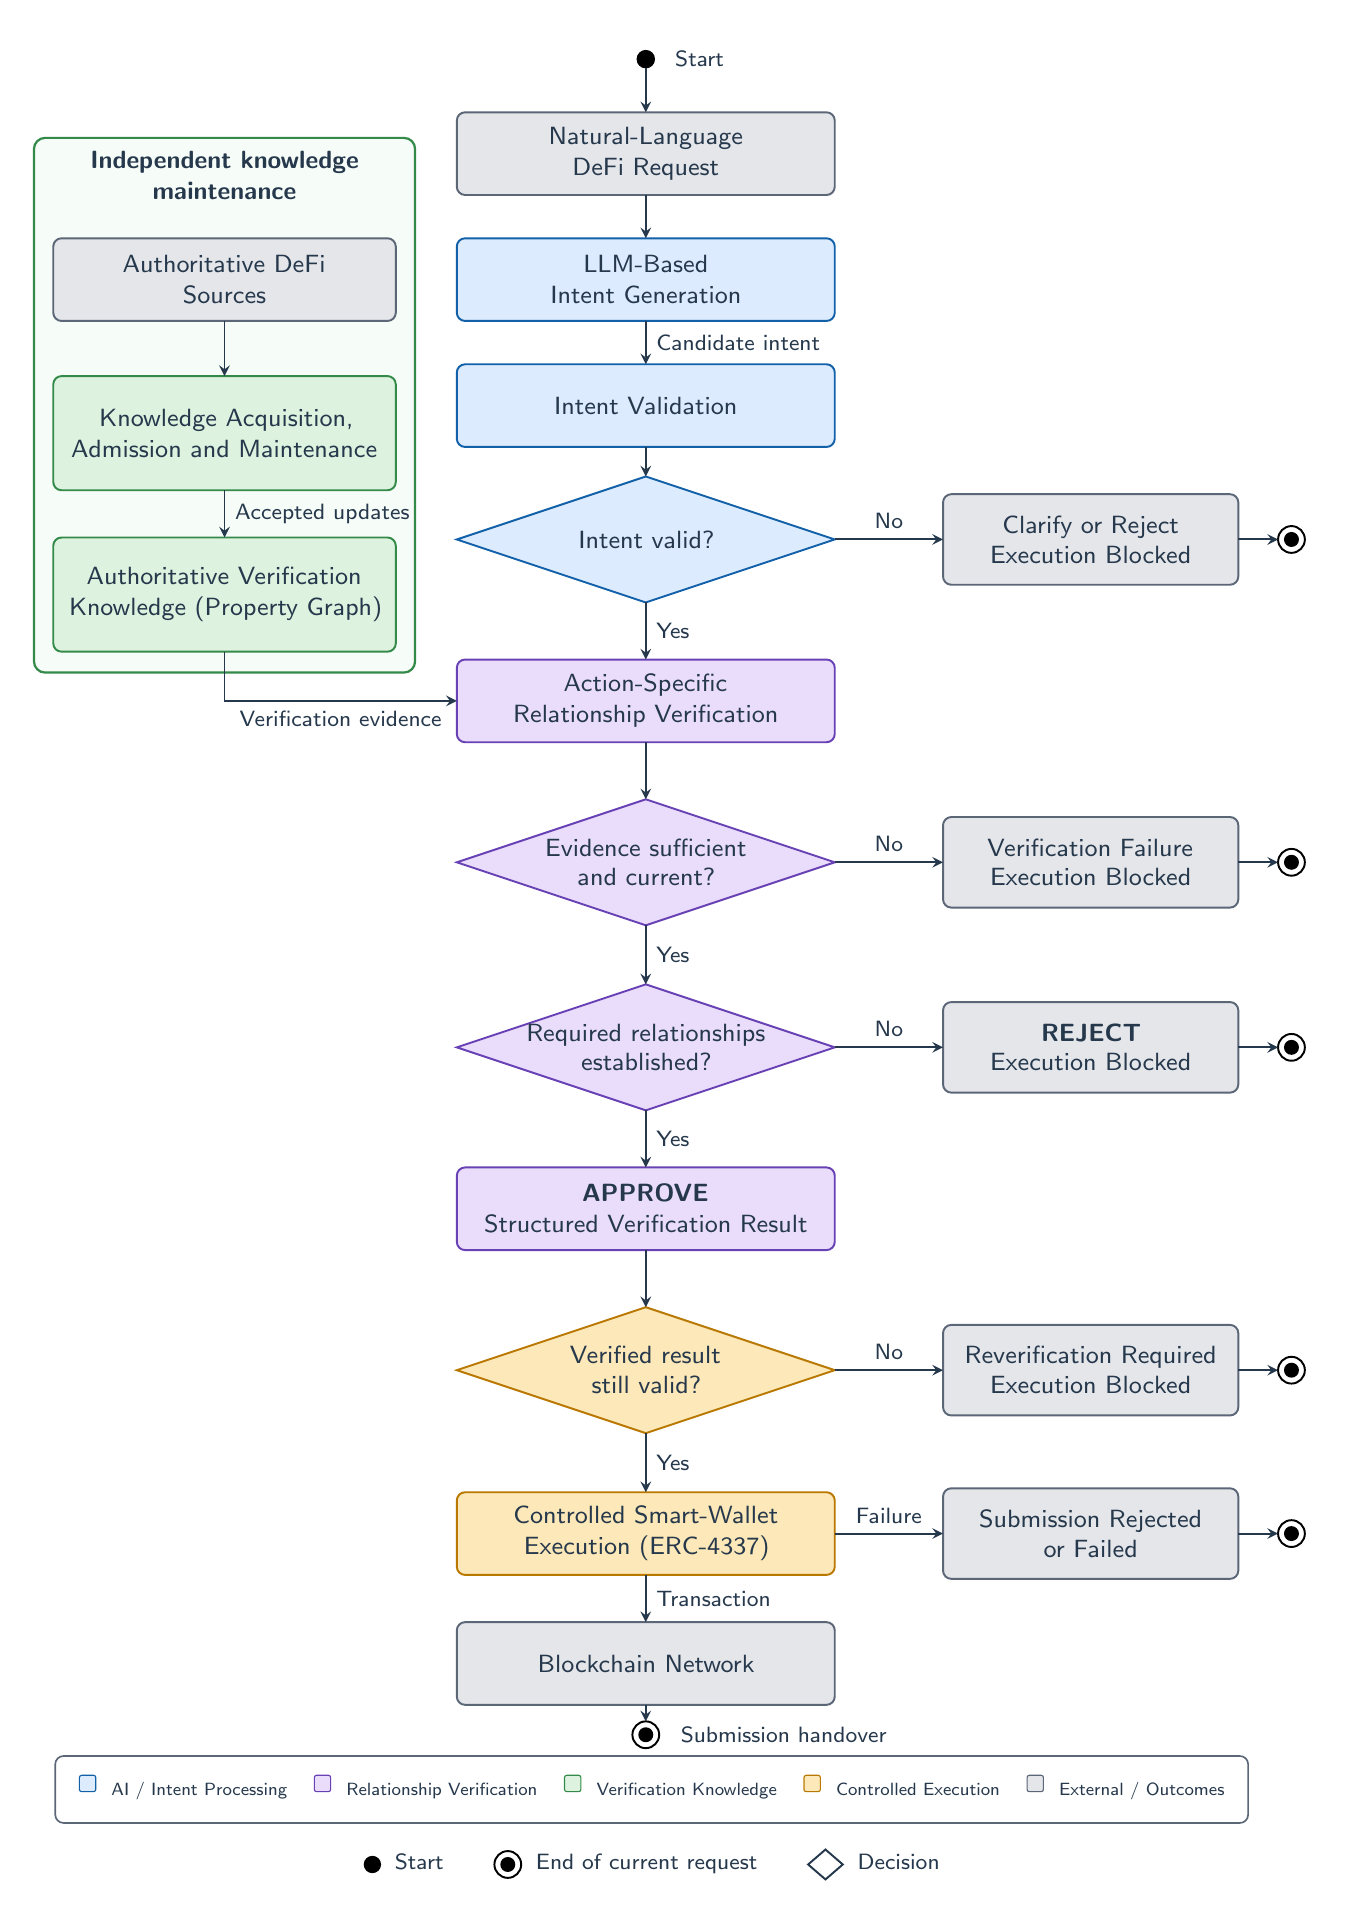
\begin{tikzpicture}[x=1cm,y=1cm,>=stealth]
\path[use as bounding box] (0,-0.20) rectangle (16.55,23.45);

% Subsystem colours, consistent with the component diagram.
\definecolor{archline}{HTML}{26384C}
\definecolor{aiborder}{HTML}{1261A8}
\definecolor{aifill}{HTML}{DCEBFE}
\definecolor{verborder}{HTML}{6842B5}
\definecolor{verfill}{HTML}{E9DDFB}
\definecolor{knowborder}{HTML}{338A49}
\definecolor{knowfill}{HTML}{DDF3DF}
\definecolor{execborder}{HTML}{B97800}
\definecolor{execfill}{HTML}{FCE8B8}
\definecolor{extborder}{HTML}{5B6677}
\definecolor{extfill}{HTML}{E4E6EA}

\tikzset{
  flowbox/.style={rectangle,rounded corners=3pt,line width=0.7pt,
    align=center,text=archline,font=\sffamily\fontsize{9.3}{11.2}\selectfont,
    text width=4.30cm,minimum width=4.80cm,minimum height=1.05cm,
    inner xsep=3pt,inner ysep=3pt,outer sep=0pt},
  ai/.style={flowbox,draw=aiborder,fill=aifill},
  verification/.style={flowbox,draw=verborder,fill=verfill},
  execution/.style={flowbox,draw=execborder,fill=execfill},
  external/.style={flowbox,draw=extborder,fill=extfill},
  knowledge/.style={flowbox,draw=knowborder,fill=knowfill,
    text width=3.95cm,minimum width=4.35cm,minimum height=1.45cm},
  outcome/.style={external,text width=3.35cm,minimum width=3.75cm,
    minimum height=1.15cm,font=\sffamily\fontsize{9}{10.8}\selectfont},
  flowarrow/.style={->,draw=archline,line width=0.70pt},
  arrowlabel/.style={font=\sffamily\fontsize{7.8}{9.2}\selectfont,
    text=archline,fill=none,inner sep=0.8pt,outer sep=0pt},
  annotation/.style={align=center,text=archline,
    font=\sffamily\fontsize{8.4}{10}\selectfont}
}

% Diamond dimensions and predictable connection points.
% Arguments: name, y, border colour, fill colour, text.
\def\FlowDecision#1#2#3#4#5{%
  \draw[draw=#3,fill=#4,line width=0.7pt]
    (7.85,{#2+0.80}) -- (10.25,#2) --
    (7.85,{#2-0.80}) -- (5.45,#2) -- cycle;
  \node[align=center,text=archline,text width=3.40cm,
    font=\sffamily\fontsize{9.0}{10.8}\selectfont,inner sep=0pt]
    at (7.85,#2) {#5};
  \coordinate (#1-north) at (7.85,{#2+0.80});
  \coordinate (#1-south) at (7.85,{#2-0.80});
  \coordinate (#1-east) at (10.25,#2);
}

% =========================================================
% Main request-processing path
% =========================================================
% UML-style initial node for one request-processing attempt.
\node[circle,draw=black,fill=black,minimum size=0.22cm,
  inner sep=0pt,outer sep=0pt] (requeststart) at (7.85,23.05) {};
\node[annotation,anchor=west] at (8.10,23.05) {Start};

\node[external] (request) at (7.85,21.85)
  {Natural-Language\\DeFi Request};
\node[ai] (generation) at (7.85,20.25)
  {LLM-Based\\Intent Generation};
\node[ai] (validation) at (7.85,18.65)
  {Intent Validation};
\FlowDecision{intent}{16.95}{aiborder}{aifill}
  {Intent valid?}

\draw[flowarrow] (requeststart.south) -- (request.north);
\draw[flowarrow] (request.south) -- (generation.north);
\draw[flowarrow] (generation.south) --
  node[arrowlabel,pos=0.5,right=3pt] {Candidate intent}
  (validation.north);
\draw[flowarrow] (validation.south) -- (intent-north);

\node[outcome] (intentfailure) at (13.50,16.95)
  {Clarify or Reject\\Execution Blocked};
\draw[flowarrow] (intent-east) --
  node[arrowlabel,pos=0.5,above=3pt] {No} (intentfailure.west);

\node[verification] (verify) at (7.85,14.90)
  {Action-Specific\\Relationship Verification};
\draw[flowarrow] (intent-south) --
  node[arrowlabel,pos=0.5,right=3pt] {Yes} (verify.north);

\FlowDecision{evidence}{12.85}{verborder}{verfill}
  {Evidence sufficient\\and current?}
\draw[flowarrow] (verify.south) -- (evidence-north);
\node[outcome] (insufficient) at (13.50,12.85)
  {Verification Failure\\Execution Blocked};
\draw[flowarrow] (evidence-east) --
  node[arrowlabel,pos=0.5,above=3pt] {No} (insufficient.west);

\FlowDecision{relationships}{10.50}{verborder}{verfill}
  {Required relationships\\established?}
\draw[flowarrow] (evidence-south) --
  node[arrowlabel,pos=0.5,right=3pt] {Yes} (relationships-north);
\node[outcome] (rejection) at (13.50,10.50)
  {\textbf{REJECT}\\Execution Blocked};
\draw[flowarrow] (relationships-east) --
  node[arrowlabel,pos=0.5,above=3pt] {No} (rejection.west);

\node[verification] (approved) at (7.85,8.45)
  {\textbf{APPROVE}\\Structured Verification Result};
\draw[flowarrow] (relationships-south) --
  node[arrowlabel,pos=0.5,right=3pt] {Yes} (approved.north);

% Includes the pre-execution check of the approved result.
\FlowDecision{valid}{6.40}{execborder}{execfill}
  {Verified result\\still valid?}
\draw[flowarrow] (approved.south) -- (valid-north);
\node[outcome] (reverify) at (13.50,6.40)
  {Reverification Required\\Execution Blocked};
\draw[flowarrow] (valid-east) --
  node[arrowlabel,pos=0.5,above=3pt] {No} (reverify.west);

\node[execution] (execution) at (7.85,4.325)
  {Controlled Smart-Wallet\\Execution (ERC-4337)};
\draw[flowarrow] (valid-south) --
  node[arrowlabel,pos=0.5,right=3pt] {Yes} (execution.north);
\node[outcome] (submissionfailure) at (13.50,4.325)
  {Submission Rejected\\or Failed};
\draw[flowarrow] (execution.east) --
  node[arrowlabel,pos=0.5,above=3pt] {Failure} (submissionfailure.west);

\node[external] (chain) at (7.85,2.675)
  {Blockchain Network};
\draw[flowarrow] (execution.south) --
  node[arrowlabel,pos=0.5,right=3pt] {Transaction} (chain.north);

% UML-style activity-final nodes end the current request attempt.
% They do not stop the independently maintained knowledge subsystem.
\def\FlowRequestEnd#1#2#3{%
  \node[circle,draw=black,fill=white,line width=0.7pt,
    minimum size=0.34cm,inner sep=0pt,outer sep=0pt]
    (#1) at (#2,#3) {};
  \fill[black] (#1.center) circle[radius=0.095cm];
}

\FlowRequestEnd{intentend}{16.05}{16.95}
\draw[flowarrow] (intentfailure.east) -- (intentend.west);

\FlowRequestEnd{evidenceend}{16.05}{12.85}
\draw[flowarrow] (insufficient.east) -- (evidenceend.west);

\FlowRequestEnd{rejectionend}{16.05}{10.50}
\draw[flowarrow] (rejection.east) -- (rejectionend.west);

\FlowRequestEnd{reverifyend}{16.05}{6.40}
\draw[flowarrow] (reverify.east) -- (reverifyend.west);

\FlowRequestEnd{submissionend}{16.05}{4.325}
\draw[flowarrow] (submissionfailure.east) -- (submissionend.west);

% This endpoint denotes handover for submission, not confirmed execution.
\FlowRequestEnd{handoverend}{7.85}{1.77}
\draw[flowarrow] (chain.south) -- (handoverend.north);
\node[annotation,anchor=west] at (8.17,1.77) {Submission handover};

% % =========================================================
% % Independent knowledge branch
% % =========================================================
% \node[external,text width=3.95cm,minimum width=4.35cm]
%   (sources) at (2.50,20.25) {Authoritative DeFi\\Sources};
% \node[knowledge] (acquisition) at (2.50,18.30)
%   {Knowledge Acquisition,\\Admission and\\Maintenance};
% \node[knowledge] (graph) at (2.50,16.25)
%   {Authoritative Verification\\Knowledge\\(Property Graph)};
% \draw[flowarrow] (sources.south) -- (acquisition.north);
% \draw[flowarrow] (acquisition.south) --
%   node[arrowlabel,pos=0.5,left=3pt] {Accepted updates} (graph.north);
% \draw[flowarrow] (graph.east) -- (5.075,16.25) --
%   (5.075,14.90) -- (verify.west);
% \node[annotation,text width=4.20cm] at (2.50,14.45)
%   {Maintained independently};

% =========================================================
% Independent knowledge maintenance
% =========================================================

% Separate panel: this process runs independently of user requests.
\draw[
  draw=knowborder,
  fill=knowfill!25!white,
  rounded corners=4pt,
  line width=0.8pt
] (0.08,15.26) rectangle (4.92,22.05);

\node[
  align=center,
  text=archline,
  font=\sffamily\bfseries\fontsize{9.3}{11.2}\selectfont,
  inner sep=0pt
] at (2.50,21.58) {Independent knowledge \\ maintenance};

% Existing knowledge stages, in their original colours.
\node[external,text width=3.95cm,minimum width=4.35cm]
  (sources) at (2.50,20.25)
  {Authoritative DeFi\\Sources};

\node[knowledge]
  (acquisition) at (2.50,18.30)
  {Knowledge Acquisition,\\Admission and Maintenance};

\node[knowledge]
  (graph) at (2.50,16.25)
  {Authoritative Verification\\Knowledge (Property Graph)};

\draw[flowarrow]
  (sources.south) -- (acquisition.north);

\draw[flowarrow]
  (acquisition.south) --
  node[arrowlabel,midway,right=3pt] {Accepted updates}
  (graph.north);

% The verifier uses evidence from the maintained graph.
% Route below the panel so the label stays clear of its border.
\draw[flowarrow]
  (graph.south) -- (2.50,14.90) --
  node[arrowlabel,midway,below=3pt] {Verification evidence}
  (verify.west);

% =========================================================
% One-row legend: aligned swatches and labels
% =========================================================
\begingroup

\def\LegendSwatch#1#2{%
  \tikz[baseline=-0.5ex]{%
    \draw[
      draw=#1,
      fill=#2,
      rounded corners=1pt,
      line width=0.5pt
    ] (0,0) rectangle (0.26,0.26);
  }%
  \hspace{4pt}%
}

\draw[draw=extborder,rounded corners=3pt,line width=0.6pt]
  (0.35,0.65) rectangle (15.50,1.50);

\node[
  font=\sffamily\fontsize{8.5}{10}\selectfont,
  text=archline,
  inner sep=0pt,
  outer sep=0pt
] at (7.925,1.075) {%
  \resizebox{14.55cm}{!}{%
    \begin{tabular}{
      @{}l@{\hspace{12pt}}
      l@{\hspace{12pt}}
      l@{\hspace{12pt}}
      l@{\hspace{12pt}}
      l@{}
    }
      \LegendSwatch{aiborder}{aifill} AI / Intent Processing
      &
      \LegendSwatch{verborder}{verfill} Relationship Verification
      &
      \LegendSwatch{knowborder}{knowfill} Verification Knowledge
      &
      \LegendSwatch{execborder}{execfill} Controlled Execution
      &
      \LegendSwatch{extborder}{extfill} External / Outcomes
    \end{tabular}%
  }%
};

\endgroup

% Compact, centred UML-style notation key
\node[
  annotation,
  inner sep=0pt,
  outer sep=0pt
] at (7.925,0.15) {%
  \begin{tabular}{
    @{}c@{\hspace{5pt}}l
    @{\hspace{18pt}}
    c@{\hspace{5pt}}l
    @{\hspace{18pt}}
    c@{\hspace{5pt}}l@{}
  }
    % Start
    \tikz[baseline=-0.5ex]{
      \fill[black] (0,0) circle[radius=0.11cm];
    }
    & Start
    &
    % End
    \tikz[baseline=-0.5ex]{
      \draw[draw=black,fill=white,line width=0.7pt]
        (0,0) circle[radius=0.17cm];
      \fill[black] (0,0) circle[radius=0.095cm];
    }
    & End of current request
    &
    % Decision
    \tikz[baseline=-0.5ex]{
      \draw[draw=archline,fill=white,line width=0.7pt]
        (0,0.19) -- (0.22,0) -- (0,-0.19) --
        (-0.22,0) -- cycle;
    }
    & Decision
  \end{tabular}%
};

\end{tikzpicture}
\endgroup%
    }
    \caption{Overall request-processing flow and supporting knowledge
    maintenance from natural-language input to controlled smart-wallet
    execution.}
    \label{fig:overall_system_flow}
\end{figure}
The language model converts the natural-language
request into a candidate intent, which must pass validation before
relationship verification begins. Validation checks whether the intent is
complete, valid, supported, and unambiguous. Requests that do not satisfy
these conditions require clarification or are rejected, and execution is
blocked.


The supporting knowledge branch shows how the authoritative property graph
is established and maintained independently of individual requests.
Information from authoritative DeFi sources, including official protocol
documentation, deployment records, and blockchain data, is acquired and
assessed for authority, consistency, and freshness before accepted entities
and relationships are added or updated. The maintained graph provides the
reference relationships and evidence used during verification.

Relationship verification evaluates the action-specific relationships
required by the validated intent. Approval requires sufficient and current
evidence establishing all mandatory relationships. If the evidence is
incomplete, stale, or unavailable, verification fails without approval.
Missing or inconsistent relationships support rejection only when the
applicable knowledge is sufficiently complete and current. An
\texttt{APPROVE} decision therefore indicates consistency with the
represented authoritative relationships within the supported scope; it does
not guarantee successful blockchain execution.

Controlled smart-wallet execution consumes the approved structured
verification result. Before submission, it checks that the
protected parameters remain unchanged, the approval has not expired, and
the referenced verification evidence remains applicable. If these conditions
are not satisfied, execution is blocked and renewed verification is required.
Even when the result remains valid, wallet authorization or execution-layer
validation may prevent successful submission. Such submission failures remain
distinct from the graph-verification decision. The blockchain endpoint in the
figure denotes submission rather than confirmation that the requested
operation has completed successfully.


It determines whether the action-specific execution relationships required
by the request can be established consistently and produces an approval,
rejection, or verification failure together with the relevant evidence
or failure reason.

Figure~\ref{fig:system_architecture} shows how the five conceptual elements
are organized into four subsystems. The arrows show the information exchanged
between them. Relationship Verification receives two inputs: a validated
intent from AI / Intent Processing, which interprets and validates the user's
request, and verification evidence from Verification Knowledge, which maintains
the authoritative property graph using records from DeFi sources. The verifier
uses this evidence to check the relationships required by the requested action.
Only an approved verification result is passed to Controlled Execution, which
checks that the approval remains valid before submitting the operation to the
blockchain network.

\begin{figure}[H]
    \centering
    \resizebox{0.98\textwidth}{!}{%
        
% \begin{tikzpicture}[x=1cm,y=1cm,>=stealth]

% % ------------------------------------------------------------
% % Bounding box
% % ------------------------------------------------------------
% \path[use as bounding box] (0,2.15) rectangle (10.55,14.55);

% % ------------------------------------------------------------
% % Colours
% % ------------------------------------------------------------
% \definecolor{archline}{HTML}{2F425A}
% \definecolor{archtext}{HTML}{1E293B}

% \definecolor{aiborder}{HTML}{1261A8}
% \definecolor{aifill}{HTML}{DCEBFE}
% \definecolor{aiboxfill}{HTML}{BFDDFD}

% \definecolor{knowborder}{HTML}{26864A}
% \definecolor{knowfill}{HTML}{E1F4E5}
% \definecolor{knowboxfill}{HTML}{CDECD2}

% \definecolor{verborder}{HTML}{3F2C8C}
% \definecolor{verfill}{HTML}{EAE6FA}
% \definecolor{verboxfill}{HTML}{DCD3FC}

% \definecolor{execborder}{HTML}{B86F00}
% \definecolor{execfill}{HTML}{FEEDCD}
% \definecolor{execboxfill}{HTML}{FEE3A8}

% \definecolor{extborder}{HTML}{44556B}
% \definecolor{extfill}{HTML}{DCDDE2}

% % ============================================================
% % Outer system boundary
% % ============================================================

% \draw[
%     draw=extborder,
%     fill=white,
%     rounded corners=0.10cm,
%     line width=0.85pt
% ] (0.55,4.5) rectangle (10.00,12.75);


% % ============================================================
% % External entities
% % ============================================================

% % User
% \draw[
%     draw=extborder,
%     fill=extfill,
%     rounded corners=0.08cm,
%     line width=0.80pt
% ] (1.15,13.55) rectangle (3.05,14.25);

% \node[
%     font=\bfseries\fontsize{5.8}{6.3}\selectfont,
%     text=archtext
% ] at (2.10,13.90)
% {User};

% % Authoritative DeFi Sources
% \draw[
%     draw=extborder,
%     fill=extfill,
%     rounded corners=0.08cm,
%     line width=0.80pt
% ] (8.10,13.55) rectangle (10.10,14.38);

% \node[
%     font=\bfseries\fontsize{4.8}{5.3}\selectfont,
%     text=archtext,
%     align=center
% ] at (9.10,13.965)
% {Authoritative\\DeFi Sources};

% % Blockchain Network
% \draw[
%     draw=extborder,
%     fill=extfill,
%     rounded corners=0.08cm,
%     line width=0.80pt
% ] (6.95,3.47) rectangle (9.35,4.20);

% \node[
%     font=\bfseries\fontsize{5.4}{5.9}\selectfont,
%     text=archtext
% ] at (8.15,3.835)
% {Blockchain Network};

% % ============================================================
% % Group containers (2 x 2 arrangement)
% % ============================================================

% % AI / Intent
% \draw[
%     draw=aiborder,
%     fill=aifill,
%     rounded corners=0.10cm,
%     line width=0.85pt
% ] (1.00,9.10) rectangle (4.55,11.85);

% \node[
%     anchor=west,
%     font=\bfseries\fontsize{6.6}{7.1}\selectfont,
%     text=archline
% ] at (1.20,11.58)
% {AI / Intent};

% % Verification Knowledge
% \draw[
%     draw=knowborder,
%     fill=knowfill,
%     rounded corners=0.10cm,
%     line width=0.85pt
% ] (5.35,9.10) rectangle (9.55,11.85);

% \node[
%     anchor=west,
%     font=\bfseries\fontsize{6.3}{6.8}\selectfont,
%     text=archline
% ] at (5.55,11.58)
% {Verification Knowledge};

% % Relationship Verification
% \draw[
%     draw=verborder,
%     fill=verfill,
%     rounded corners=0.10cm,
%     line width=0.85pt
% ] (1.00,5.35) rectangle (4.55,8.10);

% \node[
%     anchor=west,
%     font=\bfseries\fontsize{6.1}{6.6}\selectfont,
%     text=archline
% ] at (1.20,7.83)
% {Relationship Verification};

% % Controlled Execution
% \draw[
%     draw=execborder,
%     fill=execfill,
%     rounded corners=0.10cm,
%     line width=0.85pt
% ] (5.35,5.35) rectangle (9.55,8.10);

% \node[
%     anchor=west,
%     font=\bfseries\fontsize{6.4}{6.9}\selectfont,
%     text=archline
% ] at (5.55,7.83)
% {Controlled Execution};

% % ============================================================
% % Internal component boxes
% % ============================================================

% % --- AI / Intent ---
% \draw[
%     draw=aiborder,
%     fill=aiboxfill,
%     rounded corners=0.07cm,
%     line width=0.80pt
% ] (1.35,10.32) rectangle (4.20,11.05);

% \node[
%     font=\bfseries\fontsize{5.1}{5.6}\selectfont,
%     text=archtext,
%     align=center
% ] at (2.775,10.685)
% {LLM-Based Intent Generation};

% \draw[
%     draw=aiborder,
%     fill=aiboxfill,
%     rounded corners=0.07cm,
%     line width=0.80pt
% ] (1.35,9.42) rectangle (4.20,10.05);

% \node[
%     font=\bfseries\fontsize{5.0}{5.5}\selectfont,
%     text=archtext,
%     align=center
% ] at (2.775,9.735)
% {Intent Validation};

% % --- Verification Knowledge ---
% \draw[
%     draw=knowborder,
%     fill=knowboxfill,
%     rounded corners=0.07cm,
%     line width=0.80pt
% ] (5.72,10.35) rectangle (9.18,11.08);

% \node[
%     font=\bfseries\fontsize{4.9}{5.4}\selectfont,
%     text=archtext,
%     align=center
% ] at (7.45,10.715)
% {Knowledge Acquisition \& Maintenance};

% \draw[
%     draw=knowborder,
%     fill=knowboxfill,
%     rounded corners=0.07cm,
%     line width=0.80pt
% ] (5.72,9.40) rectangle (9.18,10.12);

% \node[
%     font=\bfseries\fontsize{4.9}{5.4}\selectfont,
%     text=archtext,
%     align=center
% ] at (7.45,9.76)
% {Authoritative Property Graph};

% % --- Relationship Verification ---
% \draw[
%     draw=verborder,
%     fill=verboxfill,
%     rounded corners=0.07cm,
%     line width=0.80pt
% ] (1.45,6.38) rectangle (4.10,7.12);

% \node[
%     font=\bfseries\fontsize{5.0}{5.5}\selectfont,
%     text=archtext,
%     align=center
% ] at (2.775,6.75)
% {Relationship\\ Verification \& Decision};

% % --- Controlled Execution ---
% \draw[
%     draw=execborder,
%     fill=execboxfill,
%     rounded corners=0.07cm,
%     line width=0.80pt
% ] (5.78,6.58) rectangle (9.12,7.28);

% \node[
%     font=\bfseries\fontsize{4.9}{5.4}\selectfont,
%     text=archtext,
%     align=center
% ] at (7.45,6.93)
% {Verified-Result Validity Check};

% \draw[
%     draw=execborder,
%     fill=execboxfill,
%     rounded corners=0.07cm,
%     line width=0.80pt
% ] (5.78,5.68) rectangle (9.12,6.28);

% \node[
%     font=\bfseries\fontsize{4.8}{5.3}\selectfont,
%     text=archtext,
%     align=center
% ] at (7.45,5.98)
% {ERC-4337 Smart-Wallet Execution};

% % ============================================================
% % Subtle architectural connectors
% % ============================================================

% % User -- AI / Intent
% \draw[
%     draw=archline,
%     line width=0.75pt
% ] (2.10,13.55) -- (2.10,12.20) -- (2.35,12.20) -- (2.35,11.85);

% % AI / Intent -- Relationship Verification
% \draw[
%     draw=archline,
%     line width=0.75pt
% ] (2.775,9.10) -- (2.775,8.10);

% % Authoritative DeFi Sources -- Verification Knowledge
% \draw[
%     draw=archline,
%     line width=0.75pt
% ] (9.10,13.55) -- (9.10,12.30) -- (8.70,12.30) -- (8.70,11.85);

% % Verification Knowledge -- Relationship Verification
% \draw[
%     draw=archline,
%     line width=0.75pt
% ] (5.35,9.88) -- (4.85,9.88) -- (4.85,7.05) -- (4.55,7.05);

% % Relationship Verification -- Controlled Execution
% \draw[
%     draw=archline,
%     line width=0.75pt
% ] (4.55,6.72) -- (4.95,6.72) -- (4.95,6.72) -- (5.35,6.72);

% % Controlled Execution -- Blockchain Network
% \draw[
%     draw=archline,
%     line width=0.75pt
% ] (8.20,5.35) -- (8.20,4.50) -- (8.15,4.50) -- (8.15,4.20);

% % =========================================================
% % LEGEND 
% % =========================================================

% % Outer legend rectangle
% \draw[draw=extborder,rounded corners=0.06cm,line width=0.65pt]
%   (0.23,2.30) rectangle (10.32,3.01);

% % 1 AI
% \draw[draw=aiborder,fill=aifill,rounded corners=0.03cm,line width=0.60pt]
%   (0.38,2.49) rectangle (0.70,2.81);
% \node[anchor=west,text=archline] at (0.60,2.65)
%   {\scalebox{0.38}{AI / Intent Processing}};

% % 2 Verification
% \draw[draw=verborder,fill=verfill,rounded corners=0.03cm,line width=0.60pt]
%   (2.28,2.49) rectangle (2.60,2.81);
% \node[anchor=west,text=archline] at (2.55,2.65)
%   {\scalebox{0.38}{Relationship Verification}};

% % 3 Knowledge
% \draw[draw=knowborder,fill=knowfill,rounded corners=0.03cm,line width=0.60pt]
%   (4.35,2.49) rectangle (4.67,2.81);
% \node[anchor=west,text=archline] at (4.67,2.65)
%   {\scalebox{0.38}{Verification Knowledge}};

% % 4 Execution
% \draw[draw=execborder,fill=execfill,rounded corners=0.03cm,line width=0.60pt]
%   (6.42,2.49) rectangle (6.74,2.81);
% \node[anchor=west,text=archline] at (6.74,2.65)
%   {\scalebox{0.38}{Controlled Execution}};

% % 5 External
% \draw[draw=extborder,fill=extfill,rounded corners=0.03cm,line width=0.60pt]
%   (8.42,2.49) rectangle (8.74,2.81);
% \node[anchor=west,text=archline] at (8.70,2.65)
%   {\scalebox{0.38}{External Environment}};
% \end{tikzpicture}

% All information flows point from sender to receiver; see notation key.
\begingroup
\definecolor{archline}{HTML}{2F425A}
\definecolor{archtext}{HTML}{1E293B}
\definecolor{aiborder}{HTML}{1261A8}
\definecolor{aifill}{HTML}{DCEBFE}
\definecolor{knowborder}{HTML}{26864A}
\definecolor{knowfill}{HTML}{E1F4E5}
\definecolor{verborder}{HTML}{3F2C8C}
\definecolor{verfill}{HTML}{EAE6FA}
\definecolor{execborder}{HTML}{B86F00}
\definecolor{execfill}{HTML}{FEEDCD}
\definecolor{extborder}{HTML}{44556B}
\definecolor{extfill}{HTML}{DCDDE2}

\usetikzlibrary{arrows}
\begin{tikzpicture}[x=1cm,y=1cm,
 every node/.style={text=archtext,font=\sffamily\small,align=center},
 infoflow/.style={->,>=angle 60,draw=archline,dash pattern=on 4pt off 2.5pt,line width=.78pt},
 assoc/.style={draw=archline,line width=.78pt},
 labeltext/.style={font=\sffamily\footnotesize,inner sep=2pt},
 ext/.style={draw=extborder,fill=extfill,minimum width=3.55cm,
   minimum height=.75cm,inner sep=2pt,outer sep=0pt}]
% UML component glyph: a classifier rectangle with two protruding tabs.
\def\ArchGlyph#1#2#3{%
  \begin{scope}[shift={(#1,#2)},draw=archline,line width=.6pt]
    \draw[fill=#3] (-.18,-.14) rectangle (.18,.14);
    \draw[fill=#3] (-.25,.035) rectangle (-.10,.095);
    \draw[fill=#3] (-.25,-.095) rectangle (-.10,-.035);
  \end{scope}}
% The four equal component symbols have a header and a responsibility list.
% Parameters: name, x, y, outline, fill, title, responsibilities.
\def\ArchComponent#1#2#3#4#5#6#7{%
  \node[rectangle,draw=#4,fill=#5,line width=.85pt,
     minimum width=5.10cm,minimum height=2.55cm,inner sep=0pt,
     outer sep=0pt] (#1) at (#2,#3) {};
  \begin{scope}[shift={(#1.center)}]
    \ArchGlyph{2.12}{.96}{#5}
    \node[font=\sffamily\bfseries\small,inner sep=0pt] at (0,.55) {#6};
    \draw[draw=#4,line width=.55pt] (-2.55,.08) -- (2.55,.08);
    \node[inner sep=0pt,font=\sffamily\fontsize{8.1}{10.8}\selectfont] at (0,-.57) {#7};
  \end{scope}}
\draw[draw=extborder,line width=.85pt] (0,1.7) rectangle (15.1,10.65);
\node[anchor=center,fill=white,inner xsep=5pt,font=\sffamily\bfseries\small]
 at (7.55,10.65) {AI-assisted DeFi verification system};

\ArchComponent{ai}{3.1}{8.57}{aiborder}{aifill}{AI / Intent Processing}
  {LLM-based intent generation\\Intent validation}
\ArchComponent{knowledge}{12.0}{8.57}{knowborder}{knowfill}{Verification Knowledge}
  {Acquire and maintain knowledge\\Authoritative property graph}
\ArchComponent{verifier}{3.1}{3.70}{verborder}{verfill}{Relationship Verification}
  {Action-specific relationship checks\\Verification decision and evidence}
\ArchComponent{exec}{12.0}{3.70}{execborder}{execfill}{Controlled Execution}
  {Verified-result validity check\\ERC-4337 smart-wallet execution}

% External entities.
\node[ext] (user) at (3.1,11.83) {User};
\node[ext] (sources) at (12,11.83) {Authoritative DeFi sources};
\node[ext] (chain) at (12,.61) {Blockchain network};

% Labels identify the information conveyed, rather than the calling component.
\draw[infoflow] (user.south) -- (ai.north);
\node[labeltext,anchor=west] at (3.18,11.04) {DeFi request};
\draw[infoflow] (sources.south) -- (knowledge.north);
\node[labeltext,anchor=east] at (11.91,11.04) {Protocol and deployment records};

% The verifier has two independent inputs, with distinct arrow endpoints.
\draw[infoflow] (ai.south) -- (verifier.north);
\node[labeltext,anchor=east] at (3.00,6.13) {Validated intent};
\draw[infoflow] (knowledge.south) -- (12.0,6.27) -- (4.95,6.27)
  -- (4.95,4.975);
\node[labeltext,anchor=south] at (8.48,6.34) {Verification evidence};
\draw[infoflow] (verifier.east) -- (exec.west);
\node[labeltext,anchor=south] at (7.55,3.80) {Approved\\verification result};
\draw[infoflow] (exec.south) -- (chain.north);
\node[labeltext,anchor=east] at (11.91,1.35) {Operation for submission};

% One-row colour legend, with a separate notation key underneath.
\draw[draw=extborder!65,rounded corners=2pt,line width=.55pt]
  (0,-1.88) rectangle (15.10,-.13);
\def\ArchSwatch#1#2{%
  \tikz[baseline=-.48ex]{\draw[draw=#1,fill=#2,line width=.55pt]
       (0,0) rectangle (.22,.22);}\hspace{3pt}}
\node[inner sep=0pt,font=\sffamily\fontsize{7.4}{9.2}\selectfont]
 at (7.55,-.54) {\makebox[14.50cm][s]{%
  \ArchSwatch{aiborder}{aifill}AI / Intent Processing\hfill
  \ArchSwatch{verborder}{verfill}Relationship Verification\hfill
  \ArchSwatch{knowborder}{knowfill}Verification Knowledge\hfill
  \ArchSwatch{execborder}{execfill}Controlled Execution\hfill
  \ArchSwatch{extborder}{extfill}External Environment}};
\draw[draw=extborder!35,line width=.4pt] (.27,-.96) -- (14.83,-.96);
\ArchGlyph{3.0}{-1.42}{white}
\node[labeltext,anchor=west] at (3.29,-1.42) {System component};
\draw[infoflow] (7.41,-1.42) -- (8.25,-1.42);
\node[labeltext,anchor=west] at (8.42,-1.42)
  {Information flow (sender to receiver)};
\end{tikzpicture}
\endgroup%
    }
   \caption{component diagram of the AI-assisted DeFi verification system.}
    \label{fig:system_architecture}
\end{figure}



% =========================================================
% 3.2 LLM-Based Intent Generation
% =========================================================

\section{LLM-Based Intent Generation}
\label{sec:intent_generation}

The first processing element converts the user's natural-language DeFi request
into a machine-readable representation. For example, a user may submit the
following request:

\begin{quote}
\textit{``Swap 50 USDT for WETH using Uniswap V3.''}
\end{quote}

In this example, the requested action is a swap, the protocol is Uniswap V3,
the input asset is USDT, the output asset is WETH, and the amount is 50 USDT.
Although these parameters are expressed in natural language, they must be
organized into a structured representation before they can be evaluated by
the relationship-verification component. The language model therefore
interprets the request, extracts this user-level information, and organizes
it according to a predefined structured-intent model.

Structured generation provides a predictable interface between probabilistic
language interpretation and subsequent deterministic processing. Constraining
language-model output to an expected structure can reduce variability in
generated outputs and improve their suitability for downstream processing
\cite{geng2023grammar}. Nevertheless, the generated output is treated only as
a \textit{candidate structured intent}; it is not trusted directly for
blockchain execution.

The information extracted in the example illustrates the general purpose of
the structured-intent model. At the conceptual level, a candidate intent may
contain the fields shown in Table~\ref{tab:structured_intent_fields}.

% \begin{table}[H]
% \centering
% \small
% \caption{Conceptual fields of the structured DeFi intent.}
% \label{tab:structured_intent_fields}
% \begin{tabular}{p{0.24\textwidth} p{0.70\textwidth}}
% \hline
% \textbf{Field} & \textbf{Purpose} \\
% \hline

% Action &
% Requested DeFi operation, such as swap, supply, withdraw, or borrow. \\

% Protocol &
% Requested DeFi protocol when explicitly specified or required by the
% supported operation. \\

% Network &
% Blockchain network on which the operation is intended to take place. \\

% Input / Asset &
% Asset provided, supplied, withdrawn, or borrowed depending on the action. \\

% Output Asset &
% Asset expected from an exchange operation, where applicable. \\

% Amount &
% Quantity associated with the requested operation. \\

% Recipient / Spender &
% Destination or authorization-related entity where required. \\

% Action-Specific Data &
% Additional user-level parameters required by a particular supported action. \\

% \hline
% \end{tabular}
% \end{table}

\begin{table}[H]
\centering
\small
\caption{Conceptual fields of the structured DeFi intent, with values
extracted from ``Swap 50 USDT for WETH using Uniswap V3.''}
\label{tab:structured_intent_fields}

\begin{tabular}{@{}p{0.20\textwidth} p{0.55\textwidth} p{0.16\textwidth}@{}}
\hline
\textbf{Field} & \textbf{Purpose} & \textbf{Value} \\
\hline

Action &
Requested DeFi operation, such as swap, supply, withdraw, or borrow. &
Swap \\

Protocol &
Requested DeFi protocol when explicitly specified or required by the
supported operation. &
Uniswap V3 \\

Network &
Blockchain network on which the operation is intended to take place. &
Not specified \\

Input / Asset &
Asset provided, supplied, withdrawn, or borrowed depending on the action. &
USDT \\

Output Asset &
Asset expected from an exchange operation, where applicable. &
WETH \\

Amount &
Quantity associated with the requested operation. &
50 USDT \\

Recipient / Spender &
Destination or authorization-related entity where required. &
Not specified \\

Action-Specific Data &
Additional user-level parameters required by a particular supported action. &
Not specified \\

\hline
\end{tabular}
\end{table}

The required fields depend on the requested action. A swap requires an input
asset, output asset, and amount, whereas a supply operation requires an asset
and amount but no output asset. The example request does not explicitly
specify a network. The network context may be specified by the user or
provided by the execution environment. In either case, it must be established
before relationship verification because protocol deployments and their
associated execution resources are network-specific.

The candidate intent describes \textit{what the user requests}, but does not
require the language model to select the final contract address, callable
function, liquidity pool, or transaction payload. These execution-specific
elements are resolved later using authoritative verification knowledge.
Whether the candidate intent is sufficiently complete, supported, and
unambiguous is determined by the intent-validation component described in
the following section.

% =========================================================
% 3.3 Intent Validation
% =========================================================

\section{Intent Validation}
\label{sec:intent_validation}

The candidate intent generated by the language model must be validated before
it is used for relationship verification. The purpose of this stage is to
determine whether the structured representation is sufficiently complete,
well-formed, supported, and unambiguous for deterministic processing. General schema-validation mechanisms commonly support checks such as required
properties, data types, permitted values, and numerical bounds
\cite{jsonschema2020}. In the proposed concept, these structural checks are
combined with action-specific and contextual DeFi checks.

Four categories of validation are considered:

\begin{enumerate}

    \item \textbf{Structural validation} checks whether the candidate follows
    the expected representation and contains the required fields in an
    appropriate form.

    \item \textbf{Action-specific validation} determines whether the fields
    required for the selected operation are present. For example, a swap
    requires both input and output assets, whereas a supply request requires
    an asset and amount.

    \item \textbf{Value validation} checks basic constraints on individual
    values. An amount, for example, must represent a permitted positive
    quantity.

    \item \textbf{Context and ambiguity validation} checks whether the
    requested action and network are within the supported scope and whether
    critical identifiers can be resolved unambiguously. An ambiguous asset
    identifier must not be resolved by guessing.

\end{enumerate}

If all required conditions are satisfied, the candidate becomes a
\textit{validated structured intent} and may proceed to relationship
verification. Missing, malformed, unsupported, or unresolved information
prevents further processing. Depending on the interaction model, the system may
request clarification from the user or reject the request. For the example swap request, validation checks whether the input asset, output
asset, and amount are present, whether the amount is permitted, whether the
action and network are supported, and whether the asset identifiers can be
interpreted unambiguously. It does not determine the router contract, callable
function, or liquidity pool.

Deterministic validation has a defined limitation. A structurally complete and
internally valid intent does not prove that the language model has perfectly
interpreted the user's meaning. The validation stage can identify missing,
invalid, unsupported, or ambiguous information, but it cannot generally prove
semantic equivalence between the original natural-language request and the
generated representation. The subsequent verification therefore assumes that
the validated intent represents the requested operation and focuses on whether
an authoritative execution structure can be established for it.


% =========================================================
% 3.4 Authoritative Verification Knowledge and Graph Model
% =========================================================

\section{Authoritative Verification Knowledge and Graph Model}
\label{sec:verification_knowledge}

Before a validated intent can be verified, the system requires an
authoritative representation of the execution relationships supported by
the relevant DeFi protocols. This verification knowledge is acquired,
checked, and maintained independently of the language model and individual
user requests. It represents accepted information about protocol deployments,
supported actions, contracts, callable functions, assets, liquidity pools,
lending reserves, and their relationships within the supported scope.

A graph-based representation is used because verification depends not only
on the validity of individual entities but also on their relationships.
For example, a legitimate contract or asset is insufficient if it does
not belong to the protocol deployment and action required by the current
request. The following subsections explain how this knowledge is established,
represented, and maintained for use by the relationship-verification component
described in Section~\ref{sec:relationship_verification}.

\subsection{Knowledge Acquisition and Admission}

The graph is constructed from authoritative protocol and blockchain information
rather than from execution information generated by the language model.
Relevant sources may include official deployment information, contract or
address registries, protocol-defined interfaces and documentation, and directly
verifiable on-chain protocol state. These sources provide the deployment, contract, function, asset, and
protocol-resource information required to construct the verification graph.
Table~\ref{tab:verification_sources} summarizes the main information categories
and their role in the graph. Examples include the network-specific deployment records published for Uniswap V3 and the contract addresses maintained in the Aave Address Book \cite{UniswapV3Deployments,AaveAddressBook}.

\begin{table}[H]
\centering
\caption{Conceptual sources of authoritative verification knowledge.}
\label{tab:verification_sources}
\small
\begin{tabular}{p{0.30\textwidth} p{0.29\textwidth} p{0.33\textwidth}}
\hline
\textbf{Information} &
\textbf{Source Category} &
\textbf{Purpose in the Graph} \\
\hline

Protocol deployment &
Official deployment information or registry &
Identifies network, version, and deployment context. \\

Contract information &
Official contract or address information &
Associates authoritative contracts with a deployment. \\

Callable functions &
Protocol-defined interfaces or documentation &
Associates functions with supported protocol actions. \\

Liquidity pools &
Verifiable protocol or on-chain state &
Associates pools with deployments, assets, and pool configuration. \\

Lending reserves &
Verifiable protocol or on-chain state &
Associates reserves with deployments and underlying assets. \\

Asset information &
Accepted protocol- or network-specific information &
Identifies assets in the correct blockchain context. \\

\hline
\end{tabular}
\end{table}

An important distinction is made between \textit{discovered information} and
\textit{accepted verification information}. Discovering an entity does not by
itself make that entity suitable for approving an execution. Before information
is admitted to the verification knowledge, its applicable context must be
established. Depending on the information type, this includes the originating
source, blockchain network, protocol and version, associated deployment,
synchronization time, and validity state.

Information whose source or applicable context cannot be established is not
used as positive verification evidence. The acquisition process can therefore
be summarized as:
\begin{figure}[H]
\centering
\resizebox{\linewidth}{!}{%

\begin{tikzpicture}[x=1cm,y=1cm,>=stealth]

% Colours
\definecolor{stepfill}{HTML}{F8FAFC}
\definecolor{stepborder}{HTML}{475569}
\definecolor{arrowcol}{HTML}{64748B}
\definecolor{steptext}{HTML}{1E293B}

% Authoritative Source
\draw[rounded corners=0.08cm, draw=stepborder,
      fill=stepfill, line width=0.6pt]
  (0,0) rectangle (3.2,1.1);
\node[align=center, text=steptext, font=\small]
  at (1.6,0.55)
  {\textit{Authoritative}\\\textit{Source}};

% Acquire
\draw[rounded corners=0.08cm, draw=stepborder,
      fill=stepfill, line width=0.6pt]
  (4.0,0) rectangle (6.2,1.1);
\node[align=center, text=steptext, font=\small]
  at (5.1,0.55)
  {\textit{Acquire}};

% Contextualize and Validate
\draw[rounded corners=0.08cm, draw=stepborder,
      fill=stepfill, line width=0.6pt]
  (7.55,0) rectangle (10.35,1.1);
\node[align=center, text=steptext, font=\small]
  at (8.95,0.55)
  {\textit{Contextualize}\\\textit{and Validate}};

% Admit as Verification Knowledge
\draw[rounded corners=0.08cm, draw=stepborder,
      fill=stepfill, line width=0.6pt]
  (11.7,0) rectangle (15.4,1.1);
\node[align=center, text=steptext, font=\small]
  at (13.55,0.55)
  {\textit{Admit as}\\\textit{Verification Knowledge}};

% Arrows connected to box edges
\draw[->, line width=0.7pt, draw=arrowcol]
  (3.2,0.55) -- (4.0,0.55);

\draw[->, line width=0.7pt, draw=arrowcol]
  (6.2,0.55) -- (7.55,0.55);

\draw[->, line width=0.7pt, draw=arrowcol]
  (10.35,0.55) -- (11.7,0.55);

\end{tikzpicture}%
}
\caption{Conceptual stages in establishing authoritative verification knowledge.}
\label{fig:knowledge_admission_flow}
\end{figure}

Knowledge acquisition continues after the graph is first populated and
takes place independently of individual user requests. During each
synchronization, the system compares information from authoritative sources
with the accepted records for the same network and protocol deployment.
New or changed information must meet the same admission criteria as the
original records. If a source confirms that a previously accepted
relationship is no longer valid, that relationship can no longer support
approval. If a source cannot be reached, the failed check does not renew
the freshness of the existing record.


The exact acquisition scripts, API calls, blockchain queries, and storage
operations are implementation concerns and are described in Chapter~\ref{chap:implementation}.

\subsection{Graph Model and Maintenance}
A property graph represents entities as nodes and their relationships as
edges; both can carry properties \cite{angles2018propertygraph}. In the
proposed model, nodes represent entities such as protocol deployments,
actions, contracts, and assets. The edges identify which deployment
supports an action, which contract exposes a function, and which assets
belong to a pool. Table~\ref{tab:graph_entities} summarizes the principal
entities.

\begin{table}[H]
\centering
\caption{Principal entities in the authoritative verification knowledge.}
\label{tab:graph_entities}
\small
\begin{tabular}{p{0.29\textwidth} p{0.66\textwidth}}
\hline
\textbf{Entity} & \textbf{Purpose} \\
\hline

Blockchain Network &
Defines the network context of a protocol deployment. \\

Protocol Deployment &
Represents a protocol deployment or version on a particular network. \\

Action &
Represents a supported DeFi operation such as swap, supply, withdraw, or
borrow. \\

Authoritative Contract &
Represents a contract accepted for the applicable protocol deployment. \\

Callable Function &
Represents a contract function associated with a supported action. \\

Asset &
Represents an asset in its applicable network context. \\

Liquidity Pool &
Represents an exchange resource and its participating assets and
configuration. \\

Reserve &
Represents a lending resource associated with an underlying asset. \\

Protocol-Specific Resource &
Represents additional resources required by a particular protocol or action. \\

\hline
\end{tabular}
\end{table}

Conceptually, the graph represents relationships such as a network hosting a
protocol deployment, a deployment supporting an action, a deployment using an
authoritative contract, a contract exposing a callable function, and a function
implementing an action. Additional branches associate deployments with
liquidity pools, reserves, assets, and other protocol-specific resources.

Knowledge completeness is assessed within a defined verification scope,
such as a particular network, protocol deployment, action, and resource
category. Freshness is assessed using the applicable update policy and
the recorded synchronization and validity information. A synchronization
timestamp alone does not establish that all required knowledge has been
acquired. If sufficient coverage or current applicability cannot be
established, missing relationships are treated as insufficient evidence.

Figure~\ref{fig:conceptual_graph_model} places the requested action at the
centre of the graph. The relationships around it show which deployment
supports the action, which function implements it, and which pool or
reserve can participate in it.

% \begin{figure}[H]
%     \centering
%     \includegraphics[width=0.80\textwidth]
%     {figures/conceptual_graph_model.png}
%     \caption{Conceptual action-centred graph model for representing
%     authoritative DeFi execution relationships.}
%     \label{fig:conceptual_graph_model}
% \end{figure}

\begin{figure}[H]
    \centering
    \resizebox{0.95\textwidth}{!}{%
        \begingroup
\hyphenpenalty=10000
\exhyphenpenalty=10000
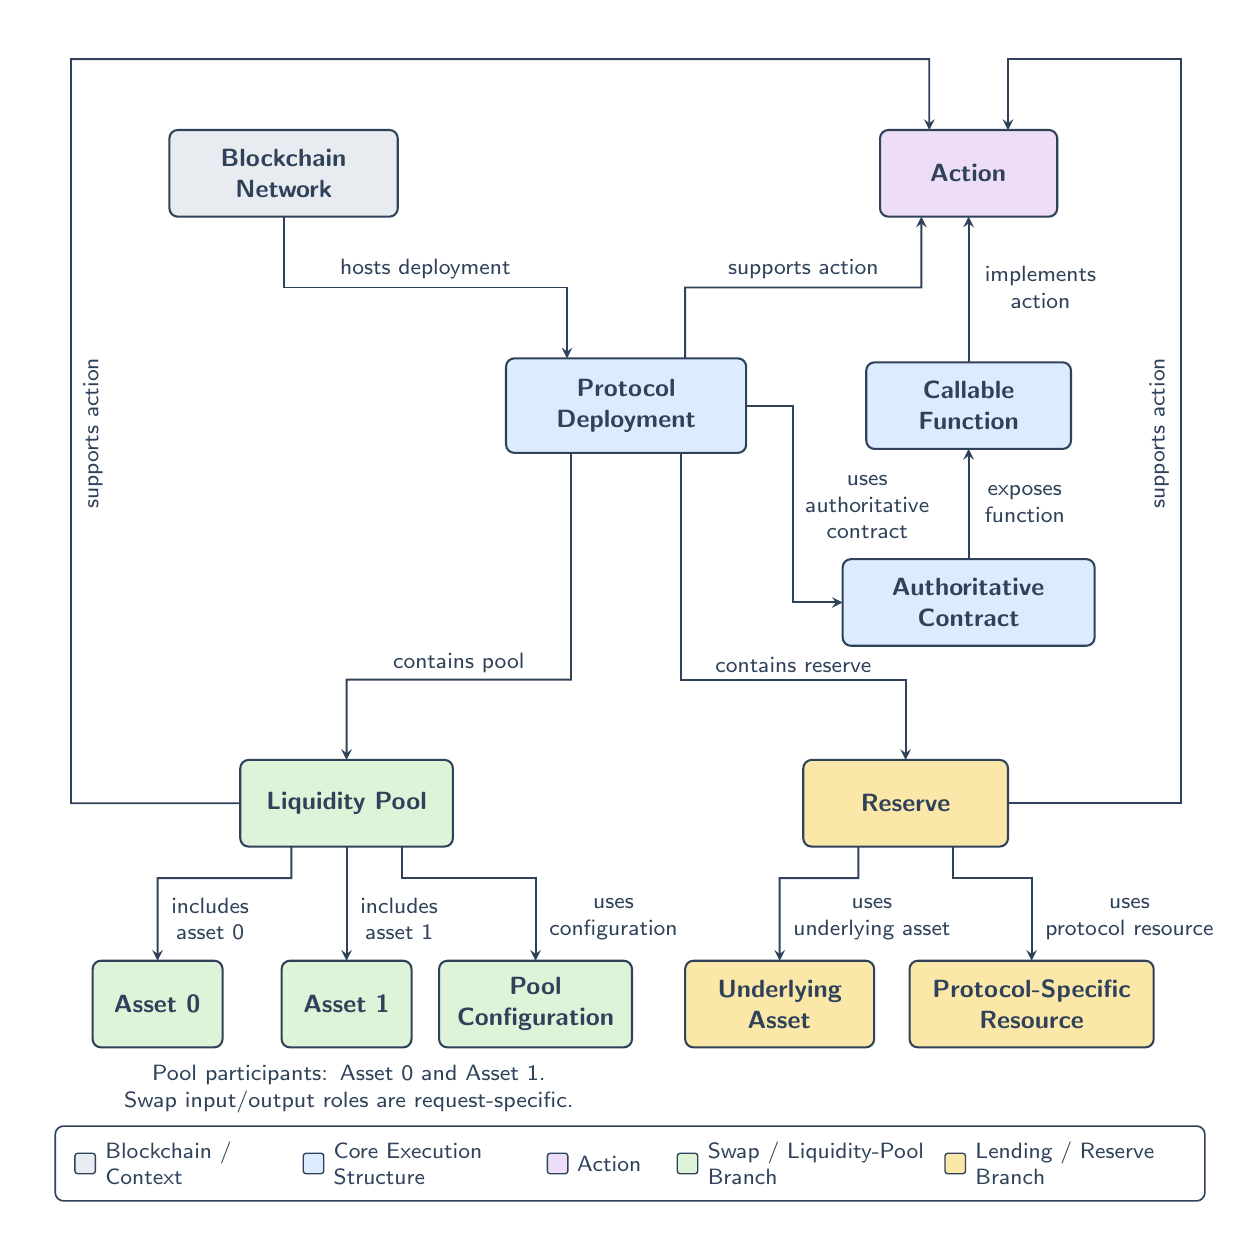
\begin{tikzpicture}[x=1cm,y=1cm,>=stealth]
\path[use as bounding box] (0,0) rectangle (15.25,15.05);

\definecolor{graphline}{HTML}{2F425A}
\definecolor{contextfill}{HTML}{E8ECF0}
\definecolor{corefill}{HTML}{DCEBFE}
\definecolor{actionfill}{HTML}{EEDDF6}
\definecolor{swapfill}{HTML}{DDF4D9}
\definecolor{lendfill}{HTML}{FBE8A9}

\tikzset{
  entity/.style={rectangle,rounded corners=3pt,draw=graphline,
    line width=0.75pt,align=center,text=graphline,
    inner xsep=4pt,inner ysep=4pt,outer sep=0pt,
    font=\sffamily\bfseries\fontsize{9.4}{11.2}\selectfont},
  relation/.style={->,draw=graphline,line width=0.70pt},
  relationlabel/.style={text=graphline,align=center,fill=white,
    inner sep=2pt,outer sep=0pt,
    font=\sffamily\fontsize{8.2}{9.6}\selectfont},
  note/.style={text=graphline,align=center,
    font=\sffamily\fontsize{8.1}{9.7}\selectfont},
  legendlabel/.style={text=graphline,anchor=west,inner sep=0pt,
    font=\sffamily\fontsize{8.0}{9.5}\selectfont}
}

% =========================================================
% Network, deployment and execution structure
% =========================================================
\node[entity,fill=contextfill,text width=2.50cm,
  minimum width=2.90cm,minimum height=1.10cm]
  (network) at (3.25,13.20) {Blockchain\\Network};
\node[entity,fill=actionfill,text width=1.95cm,
  minimum width=2.25cm,minimum height=1.10cm]
  (action) at (11.95,13.20) {Action};
\node[entity,fill=corefill,text width=2.65cm,
  minimum width=3.05cm,minimum height=1.20cm]
  (deployment) at (7.60,10.25) {Protocol\\Deployment};
\node[entity,fill=corefill,text width=2.20cm,
  minimum width=2.60cm,minimum height=1.10cm]
  (function) at (11.95,10.25) {Callable\\Function};
\node[entity,fill=corefill,text width=2.80cm,
  minimum width=3.20cm,minimum height=1.10cm]
  (contract) at (11.95,7.75) {Authoritative\\Contract};

% =========================================================
% Swap and lending branches: aligned parent and leaf rows
% =========================================================
\node[entity,fill=swapfill,text width=2.30cm,
  minimum width=2.70cm,minimum height=1.10cm]
  (pool) at (4.05,5.20) {Liquidity Pool};
\node[entity,fill=lendfill,text width=2.20cm,
  minimum width=2.60cm,minimum height=1.10cm]
  (reserve) at (11.15,5.20) {Reserve};

\node[entity,fill=swapfill,text width=1.35cm,
  minimum width=1.65cm,minimum height=1.10cm]
  (assetZero) at (1.65,2.65) {Asset 0};
\node[entity,fill=swapfill,text width=1.35cm,
  minimum width=1.65cm,minimum height=1.10cm]
  (assetOne) at (4.05,2.65) {Asset 1};
\node[entity,fill=swapfill,text width=2.15cm,
  minimum width=2.45cm,minimum height=1.10cm]
  (poolConfig) at (6.45,2.65) {Pool\\Configuration};
\node[entity,fill=lendfill,text width=2.00cm,
  minimum width=2.40cm,minimum height=1.10cm]
  (assetLend) at (9.55,2.65) {Underlying\\Asset};
\node[entity,fill=lendfill,text width=2.75cm,
  minimum width=3.10cm,minimum height=1.10cm]
  (resource) at (12.75,2.65) {Protocol-Specific\\Resource};

% =========================================================
% The two outer return paths enter Action through separate top ports.
\tikzset{edgecaption/.style={relationlabel,fill=none,inner sep=1pt}}
\draw[relation] (pool.west) -- (0.55,5.20) -- (0.55,14.65)
  -- (11.45,14.65) -- ([xshift=-0.50cm]action.north);
\draw[relation] (reserve.east) -- (14.65,5.20) -- (14.65,14.65)
  -- (12.45,14.65) -- ([xshift=0.50cm]action.north);
\node[edgecaption,rotate=90] at (0.83,9.90) {supports action};
\node[edgecaption,rotate=90] at (14.37,9.90) {supports action};

% Core execution structure.
\draw[relation] (network.south) -- (3.25,11.75)
  -- (6.85,11.75) -- ([xshift=-0.75cm]deployment.north);
\node[edgecaption,anchor=south] at (5.05,11.82) {hosts deployment};
\draw[relation] ([xshift=0.75cm]deployment.north) -- (8.35,11.75)
  -- (11.35,11.75) -- ([xshift=-0.60cm]action.south);
\node[edgecaption,anchor=south] at (9.85,11.82) {supports action};
\draw[relation] (function.north) -- (action.south);
\node[edgecaption,anchor=west] at (12.12,11.75) {implements\\action};
\draw[relation] (contract.north) -- (function.south);
\node[edgecaption,anchor=west] at (12.12,9.00) {exposes\\function};
\draw[relation] (deployment.east) -- (9.72,10.25)
  -- (9.72,7.75) -- (contract.west);
\node[edgecaption,anchor=west] at (9.84,8.96) {uses\\authoritative\\contract};

% Mirrored membership routes: separate departure ports, common bend height.
\draw[relation] ([xshift=-0.70cm]deployment.south) -- (6.90,6.77)
  -- (4.05,6.77) -- (pool.north);
\draw[relation] ([xshift=0.70cm]deployment.south) -- (8.30,6.77)
  -- (11.15,6.77) -- (reserve.north);
\node[edgecaption,anchor=south] at (5.475,6.82) {contains pool};
\node[edgecaption,anchor=south] at (9.725,6.82) {contains reserve};

% Each leaf has its own edge (no shared stem or ambiguous junction).
\draw[relation] ([xshift=-0.70cm]pool.south) -- (3.35,4.25)
  -- (1.65,4.25) -- (assetZero.north);
\draw[relation] (pool.south) -- (assetOne.north);
\draw[relation] ([xshift=0.70cm]pool.south) -- (4.75,4.25)
  -- (6.45,4.25) -- (poolConfig.north);
\draw[relation] ([xshift=-0.60cm]reserve.south) -- (10.55,4.25)
  -- (9.55,4.25) -- (assetLend.north);
\draw[relation] ([xshift=0.60cm]reserve.south) -- (11.75,4.25)
  -- (12.75,4.25) -- (resource.north);
\node[edgecaption,anchor=west] at (1.79,3.73) {includes\\asset 0};
\node[edgecaption,anchor=west] at (4.19,3.73) {includes\\asset 1};
\node[edgecaption,anchor=west] at (6.59,3.73) {uses\\configuration};
\node[edgecaption,anchor=west] at (9.69,3.73) {uses\\underlying asset};
\node[edgecaption,anchor=west] at (12.89,3.73) {uses\\protocol resource};

% Asset roles are request-specific, not additional graph entities.
\node[note,text width=7.00cm] at (4.05,1.57)
  {Pool participants: Asset 0 and Asset 1.\\
   Swap input/output roles are request-specific.};

% =========================================================
% One-row legend: conceptual roles, not approval or trust status
% =========================================================
\draw[draw=graphline,rounded corners=3pt,line width=0.6pt]
  (0.35,0.15) rectangle (14.95,1.10);
\foreach \GraphLegendX/\GraphLegendColour/\GraphLegendWidth/\GraphLegendText in {
  0.60/contextfill/2.35/{Blockchain /\\Context},
  3.50/corefill/2.55/{Core Execution\\Structure},
  6.60/actionfill/1.15/{Action},
  8.25/swapfill/2.75/{Swap / Liquidity-Pool\\Branch},
  11.65/lendfill/2.55/{Lending / Reserve\\Branch}}
{
  \draw[draw=graphline,fill=\GraphLegendColour,rounded corners=1pt,line width=0.5pt]
    (\GraphLegendX,0.495) rectangle ({\GraphLegendX+0.26},0.755);
  \node[legendlabel,text width=\GraphLegendWidth cm,align=left]
    at ({\GraphLegendX+0.38},0.625) {\GraphLegendText};
}
\end{tikzpicture}
\endgroup%
    }
    \caption{Conceptual action-centred property graph for authoritative
    DeFi verification knowledge.}
    \label{fig:conceptual_graph_model}
\end{figure}

The graph is intentionally action-centred because different operations require
different connected structures. A swap may require relationships among the
deployment, swap action, routing contract, function, liquidity pool, and
requested assets. A lending operation may instead require the deployment,
lending action, protocol contract, function, reserve, and underlying asset. The existence of a resource does not automatically imply that every action is
available for it. For example, the presence of an asset as a lending reserve
establishes reserve membership but does not by itself establish that supply or
borrowing is currently enabled. Action availability must therefore be
represented or verified separately from resource membership.

The W3C PROV-O ontology describes how information is derived from a source
and how its invalidation can be recorded \cite{w3cPROVO2013}. In the
proposed graph, each verification record identifies its source, the network
and protocol deployment to which it applies, its synchronization time, and
its validity state. The knowledge-maintenance process must therefore support both updates and
invalidation. A previously accepted contract, pool, reserve, or relationship
must not remain usable as positive verification evidence after it is no longer
applicable. New protocols, networks, assets, or actions can be incorporated by
extending the graph with additional accepted entities and relationships without
changing the overall verification principle.


% =========================================================
% 3.5 Relationship Verification and Decision
% =========================================================

\section{Relationship Verification and Decision}
\label{sec:relationship_verification}

After intent validation, the system determines whether the requested operation
can be mapped to an accepted execution structure. Unlike intent validation,
which evaluates the structured request itself, relationship verification
evaluates the execution relationships required to realize that request. The requested action determines the relationship pattern that must be
established. Conceptually, verification consists of identifying the applicable
execution context, determining the required relationship pattern, resolving the
corresponding entities from the authoritative graph, and evaluating whether all
mandatory relationships are supported by valid evidence.

% \subsection{Action-Specific Relationship Verification}

% Relationship verification determines whether the requested DeFi operation
% is supported by a consistent set of execution relationships in the
% authoritative property graph. The relationships that must be established
% depend on the requested action.

% Consider the example introduced in Section~\ref{sec:intent_generation}:

% \begin{quote}
% \textit{``Swap 50 USDT for WETH using Uniswap V3.''}
% \end{quote}

% After intent validation, the verifier uses the requested action, protocol,
% network, and assets to identify the required execution relationships.
% For this swap, it must establish that the applicable network hosts a
% Uniswap V3 deployment supporting the swap action. It must also identify
% an authoritative contract with a callable swap function and verify that
% a compatible liquidity pool supports the requested asset pair and
% applicable pool configuration.

% These checks establish whether the requested operation has a supported
% execution structure. The amount of 50 USDT remains a user-provided
% parameter; the graph is used to resolve and verify execution-specific
% information rather than to modify the requested operation.

% Other DeFi actions require different relationships. For example, a
% lending operation requires evidence of an applicable lending deployment,
% an authoritative contract and function for the requested action, and
% a reserve supporting the requested asset. The representative requirements
% for swap, supply, and borrow operations are summarized in
% Table~\ref{tab:verification_patterns}.

% \begin{table}[H]
% \centering
% \caption{Representative action-specific relationship requirements.}
% \label{tab:verification_patterns}

% \small

% \begin{tabular}{p{0.18\textwidth} p{0.77\textwidth}}
% \hline
% \textbf{Action} & \textbf{Required Verification Evidence} \\
% \hline

% Swap &
% The applicable network and protocol deployment support the swap action.
% An authoritative contract provides a callable swap function, and a
% compatible liquidity pool supports the requested asset pair and
% applicable pool configuration. \\

% Supply &
% The applicable network and lending deployment support the supply action.
% An authoritative contract provides a callable supply function, and a
% lending reserve supports the requested asset and supply operation. \\

% Borrow &
% The applicable network and lending deployment support the borrow action.
% An authoritative contract provides a callable borrow function, and a
% lending reserve supports the requested asset and borrow operation. \\

% \hline
% \end{tabular}
% \end{table}

% The verifier evaluates these requirements as connected relationships
% within the same network and protocol deployment. For example, an
% authoritative contract and a compatible liquidity pool cannot establish
% a valid swap execution structure if they belong to different deployments.
% An operation can therefore be approved only when all mandatory
% relationships for its action are established consistently.


% \subsection{Decision and Traceable Verification Result}

% The verification result directly determines the decision. A separate
% probabilistic decision component is not required.

% The conceptual approval rule is:

% \begin{quote}
% \textit{A request is approved only when the structured intent is valid and
% sufficient accepted evidence exists for every mandatory relationship required
% by the requested action and execution context.}
% \end{quote}

% An \textbf{APPROVE} result is produced only when all mandatory execution
% relationships can be established consistently using valid authoritative
% verification knowledge. If the available evidence establishes that the requested execution structure
% is unsupported or inconsistent, the verifier produces a \textbf{REJECT}
% result. For example, the requested action may not be supported by the
% applicable protocol deployment, or the required contract, function, and
% protocol resources may not form a consistent execution structure.

% The verifier obtains its evidence from the authoritative property graph
% described in Section~\ref{sec:verification_knowledge}. If the required
% information is missing, outdated, or unavailable, the verifier cannot
% establish whether the requested execution structure is supported. This
% condition is reported as a \textbf{verification failure}, rather than
% assuming that missing relationships are valid or treating incomplete
% knowledge as proof that the operation is unsupported. The absence of a matching relationship is treated as evidence of an
% unsupported operation only when the applicable verification knowledge is
% sufficiently complete and current for that check. Otherwise, the absence
% is treated as insufficient evidence and results in a verification failure.

% Both rejection and verification failure prevent blockchain execution.
% A request may proceed only after all mandatory relationships have been
% established using valid authoritative evidence.

% Figure~\ref{fig:verification_outcome_examples} illustrates these three
% outcomes for the same hypothetical validated swap request. Sufficient,
% current, and valid evidence establishing all mandatory relationships leads
% to approval. Complete and current knowledge, together with valid evidence
% establishing that the deployment does not support the requested action,
% leads to rejection. Stale or unavailable evidence instead produces a
% verification failure because action support cannot be established. Approval
% allows the verified result to proceed to the controlled execution checks;
% it does not guarantee successful blockchain execution.

% \begin{figure}[H]
%     \centering
%     \resizebox{0.98\linewidth}{!}{%
%         % % Requires \usepackage{tikz}. Include inside a figure environment.
% % Illustrative alternatives for the same validated request.
% \begingroup
% \begin{tikzpicture}[x=1cm,y=1cm,>=stealth]
% \definecolor{outcometext}{HTML}{1E293B}
% \definecolor{outcomeline}{HTML}{475569}
% \definecolor{outcomeneutral}{HTML}{F8FAFC}
% \definecolor{outcomeapprove}{HTML}{26864A}
% \definecolor{outcomeapprovefill}{HTML}{E1F4E5}
% \definecolor{outcomereject}{HTML}{A43A3A}
% \definecolor{outcomerejectfill}{HTML}{FBE8E8}
% \definecolor{outcomefailure}{HTML}{B86F00}
% \definecolor{outcomefailurefill}{HTML}{FEEDCD}

% \tikzset{
%   outcomeExampleBox/.style={draw=outcomeline,fill=outcomeneutral,
%     rounded corners=2pt,line width=0.65pt,align=center,text=outcometext,
%     inner sep=3pt,outer sep=0pt,font=\sffamily\fontsize{8.5}{10.5}\selectfont},
%   outcomeExampleText/.style={align=center,text=outcometext,inner sep=0pt,
%     font=\sffamily\fontsize{8.5}{10.5}\selectfont},
%   outcomeExampleArrow/.style={->,draw=outcomeline,line width=0.75pt}
% }

% \path[use as bounding box] (-0.05,0.60) rectangle (14.35,7.65);

% % A common request makes the difference in evidence explicit.
% \node[outcomeExampleBox,text width=13.15cm,minimum height=1.0cm]
%   (exampleRequest) at (7.15,7.08)
%   {\textbf{Validated request: swap 50 USDT for WETH}\\
%    Specified protocol deployment and blockchain network};

% \node[outcomeExampleText,font=\sffamily\fontsize{8}{9.5}\selectfont]
%   at (7.15,6.26)
%   {Three illustrative evidence conditions for the same request};

% % Equal panels and evidence boxes.
% \draw[draw=outcomeline,rounded corners=3pt,line width=0.6pt]
%   (0,0.72) rectangle (4.40,5.95);
% \draw[draw=outcomeline,rounded corners=3pt,line width=0.6pt]
%   (4.95,0.72) rectangle (9.35,5.95);
% \draw[draw=outcomeline,rounded corners=3pt,line width=0.6pt]
%   (9.90,0.72) rectangle (14.30,5.95);

% \node[outcomeExampleText,font=\sffamily\bfseries\fontsize{9}{11}\selectfont]
%   at (2.20,5.57) {Relationships established};
% \node[outcomeExampleText,font=\sffamily\bfseries\fontsize{9}{11}\selectfont]
%   at (7.15,5.57) {Unsupported action};
% \node[outcomeExampleText,font=\sffamily\bfseries\fontsize{9}{11}\selectfont]
%   at (12.10,5.57) {Insufficient valid evidence};

% \node[outcomeExampleBox,text width=3.65cm,minimum height=1.80cm]
%   (approveEvidence) at (2.20,4.30)
%   {Sufficient, current, valid\\
%    evidence establishes all\\
%    mandatory execution\\
%    relationships.};
% \node[outcomeExampleBox,text width=3.65cm,minimum height=1.80cm]
%   (rejectEvidence) at (7.15,4.30)
%   {Knowledge is complete\\
%    and current. Valid evidence\\
%    establishes that the swap\\
%    is unsupported.};
% \node[outcomeExampleBox,text width=3.65cm,minimum height=1.80cm]
%   (failureEvidence) at (12.10,4.30)
%   {Required deployment\\
%    evidence is stale or\\
%    unavailable; action support\\
%    cannot be established.};

% % Outcome boxes have identical dimensions.
% \node[outcomeExampleBox,text width=3.65cm,minimum height=1.05cm,
%   draw=outcomeapprove,fill=outcomeapprovefill,
%   font=\sffamily\bfseries\fontsize{9}{11}\selectfont]
%   (approveOutcome) at (2.20,2.53) {APPROVE};
% \node[outcomeExampleBox,text width=3.65cm,minimum height=1.05cm,
%   draw=outcomereject,fill=outcomerejectfill,
%   font=\sffamily\bfseries\fontsize{9}{11}\selectfont]
%   (rejectOutcome) at (7.15,2.53) {REJECT};
% \node[outcomeExampleBox,text width=3.65cm,minimum height=1.05cm,
%   draw=outcomefailure,fill=outcomefailurefill,
%   font=\sffamily\bfseries\fontsize{9}{11}\selectfont]
%   (failureOutcome) at (12.10,2.53) {VERIFICATION\\FAILURE};

% \draw[outcomeExampleArrow] (approveEvidence.south) -- (approveOutcome.north);
% \draw[outcomeExampleArrow] (rejectEvidence.south) -- (rejectOutcome.north);
% \draw[outcomeExampleArrow] (failureEvidence.south) -- (failureOutcome.north);

% \node[outcomeExampleText,text width=3.80cm] at (2.20,1.43)
%   {Forward approved result\\to controlled execution checks};
% \node[outcomeExampleText,text width=3.80cm] at (7.15,1.43)
%   {Block execution;\\report the unsupported action};
% \node[outcomeExampleText,text width=3.80cm] at (12.10,1.43)
%   {Block execution;\\report insufficient valid evidence};
% \end{tikzpicture}
% \endgroup
\begingroup
\definecolor{vInk}{HTML}{24394F}
\definecolor{vLine}{HTML}{506479}
\definecolor{vNode}{HTML}{F3F6FA}
\definecolor{vOk}{HTML}{206642}
\definecolor{vOkBg}{HTML}{E4F2E9}
\definecolor{vNo}{HTML}{923537}
\definecolor{vNoBg}{HTML}{F8E9E7}
\begin{tikzpicture}[x=1cm,y=1cm,>=stealth,
  every node/.style={font=\sffamily\small,text=vInk,align=center},
  vertex/.style={draw=vLine,fill=vNode,rounded corners=2pt,
    line width=.55pt,inner xsep=5pt,inner ysep=4pt,outer sep=0pt},
  edge/.style={->,draw=vLine,line width=.65pt},
  verb/.style={font=\sffamily\footnotesize,inner sep=1.3pt},
  title/.style={font=\sffamily\bfseries\small}]
\node[title] at (7.35,9.75) {Validated intent: swap 50 USDT for WETH on Uniswap V3};
\node[font=\sffamily\footnotesize] at (7.35,9.27)
  {Sepolia context\enspace$\cdot$\enspace Direct swap\enspace$\cdot$\enspace One eligible pool in this example};
\foreach \dx/\lettertag/\heading/\otherasset/\decision/\ink/\tint in {
  0/A/Matching pool pair/WETH/APPROVE/vOk/vOkBg,
  7.55/B/Conflicting pool pair/USDC/REJECT/vNo/vNoBg}{
  \begin{scope}[xshift=\dx cm]
    \draw[draw=vLine!55,rounded corners=3pt,line width=.55pt]
      (0,0) rectangle (7.15,8.85);
    \node[title] at (3.575,8.50) {\lettertag.\enspace \heading};
    \node[vertex] (net) at (3.575,7.75) {Sepolia};
    \node[vertex] (dep) at (3.575,6.45) {Uniswap V3 deployment};
    \node[vertex] (router) at (1.48,4.90) {Router};
    \node[vertex] (pool) at (5.27,4.90) {Pool $P$};
    \node[vertex] (func) at (1.48,3.48) {Swap function};
    \node[vertex] (action) at (1.48,2.05) {Swap action};
    \node[vertex] (assetA) at (4.23,3.00) {USDT};
    \node[vertex,draw=\ink,fill=\tint,text=\ink,font=\sffamily\bfseries\small]
      (assetB) at (6.28,3.00) {\otherasset};
    \draw[edge] (net.south) -- node[verb,right] {hosts} (dep.north);
    \draw[edge] (dep.south) -- (3.575,5.98) -| (router.north);
    \draw[edge] (dep.south) -- (3.575,5.98) -| (pool.north);
    \node[verb,right] at (1.48,5.66) {uses};
    \node[verb,left] at (5.27,5.66) {contains};
    \draw[edge] (router.south) -- node[verb,right] {exposes} (func.north);
    \draw[edge] (func.south) -- node[verb,right] {implements} (action.north);
    \draw[edge] (pool.south) -- (5.27,4.02) -- (4.23,4.02) -- (assetA.north);
    \draw[edge] (pool.south) -- (5.27,4.02) -- (6.28,4.02) -- (assetB.north);
    \node[verb] at (5.27,3.70) {includes};
    \node[font=\sffamily\footnotesize] at (5.25,2.15) {Required output: WETH};
    \draw[draw=vLine!35] (.30,1.49) -- (6.85,1.49);
    \node[title,text=\ink] at (3.575,1.04) {\decision};
    \def\firstpanel{A}
    \ifx\lettertag\firstpanel
      \node at (3.575,.48) {Both requested assets belong to $P$.};
    \else
      \node at (3.575,.48) {$P$ pairs USDT with USDC, not WETH.};
    \fi
  \end{scope}}
\end{tikzpicture}
\endgroup%
%     }
%     \caption{Illustrative verification outcomes for a DeFi request:
% approval, rejection, and verification failure.}
%     \label{fig:verification_outcome_examples}
% \end{figure}

% The result also records information required for traceability. Depending on the
% outcome, this includes:

% \begin{itemize}
%     \item the approval, rejection, or verification-failure decision;
%     \item a reason identifying the relevant failed or satisfied condition;
%     \item the entities and relationships relevant to the decision;
%     \item the execution information resolved from authoritative knowledge;
%     \item the user-provided parameters covered by the verification;
%     \item the authoritative evidence used; and
%     \item the time and validity context of the result.
% \end{itemize}

% For an approved operation, this result binds the validated intent to the
% resolved execution structure. It may therefore contain the network, protocol
% deployment, target contract, callable function, relevant assets, pool or
% reserve, amount, recipient or spender where applicable, and other protected
% action-specific parameters. For a rejected request, the reason should identify the failed condition without
% claiming information that was never resolved. For example, if no authoritative
% contract can be established, the result should report that condition rather
% than describing a mismatch with a particular contract. A successful result is valid only for the operation and context that were
% actually verified. Changes to protected parameters or invalidation of the
% underlying evidence require another verification before execution.

% Figure~\ref{fig:verification_sequence} illustrates the interaction between
% intent validation, relationship verification and decision, authoritative
% verification knowledge, and the request controller. \\
% The sequence starts once the candidate intent has successfully passed
% deterministic validation. The validated intent is then forwarded to the
% relationship-verification component, which identifies the relationships that
% must hold for the requested DeFi action. Using the action, protocol, network,
% and asset information from the intent, the verifier queries the authoritative
% graph for the corresponding deployment, contract, callable function, and
% protocol-specific resources such as a liquidity pool or lending reserve. The
% graph returns the available verification evidence, which is evaluated as one
% connected execution structure rather than as isolated entities. If sufficient, current, and valid evidence establishes all mandatory
% relationships within the same execution context, the verifier returns an
% approved structured verification result to the request controller,
% including the resolved execution information. If the applicable knowledge
% is sufficiently complete and current but the required relationships cannot
% be established, the verifier returns a rejection with the supporting reason
% and evidence. Otherwise, insufficient, invalid, stale, or unavailable
% evidence produces a verification failure rather than a supported rejection.

% \begin{figure}[H]
%     \centering
%     \resizebox{0.95\textwidth}{!}{%
%         
% \begingroup
% \hyphenpenalty=10000
% \exhyphenpenalty=10000
% \begin{tikzpicture}[x=1cm,y=1cm,>=stealth]
% \path[use as bounding box] (0.15,0.20) rectangle (16.35,20.35);

% % Original colours preserved exactly.
% \definecolor{seqtext}{HTML}{1E293B}
% \definecolor{seqborder}{HTML}{475569}
% \definecolor{seqarrow}{HTML}{64748B}
% \definecolor{seqfill}{HTML}{DBEAFE}

% \tikzset{
%   seqparticipant/.style={rectangle,rounded corners=2.5pt,
%     draw=seqborder,fill=seqfill,line width=0.75pt,
%     minimum width=3.50cm,minimum height=1.80cm,text width=3.10cm,
%     align=center,text=seqtext,inner xsep=3pt,inner ysep=3pt,
%     outer sep=0pt,font=\sffamily\bfseries\fontsize{9.3}{11.2}\selectfont},
%   seqlifeline/.style={draw=seqarrow,dash pattern=on 3pt off 1.8pt,line width=0.72pt},
%   seqmessage/.style={->,draw=seqarrow,line width=0.80pt},
%   seqreturn/.style={seqmessage,dashed,line width=0.75pt},
%   seqactivation/.style={draw=seqborder,fill=seqfill,line width=0.65pt},
%   seqmessagetext/.style={text=seqtext,align=center,fill=none,
%     inner sep=2pt,outer sep=0pt,
%     font=\sffamily\fontsize{9.0}{10.8}\selectfont},
%   seqselftext/.style={seqmessagetext,anchor=west,align=left,
%     text width=2.80cm,font=\sffamily\fontsize{8.6}{10.3}\selectfont},
%   seqguard/.style={anchor=north west,text=seqtext,align=left,
%     text width=3.40cm,fill=none,inner sep=2pt,outer sep=0pt,
%     font=\sffamily\fontsize{8.4}{10.0}\selectfont}
% }

% % Equal participant widths, heights and horizontal spacing.
% \def\SeqIntentX{2.05}
% \def\SeqVerifyX{6.10}
% \def\SeqGraphX{10.15}
% \def\SeqControllerX{14.20}

% \node[seqparticipant] (intent) at (\SeqIntentX,19.30)
%   {Intent\\Validation};
% \node[seqparticipant] (verifier) at (\SeqVerifyX,19.30)
%   {Relationship\\Verification \&\\Decision};
% \node[seqparticipant] (knowledge) at (\SeqGraphX,19.30)
%   {Authoritative\\Verification Knowledge\\
%    {\mdseries\fontsize{8.4}{10}\selectfont Property Graph}};
% \node[seqparticipant] (controller) at (\SeqControllerX,19.30)
%   {Request\\Controller};

% % Lifelines start at the bottom of the participant boxes.
% \draw[seqlifeline] (intent.south) -- (\SeqIntentX,1.65);
% \draw[seqlifeline] (verifier.south) -- (\SeqVerifyX,1.65);
% \draw[seqlifeline] (knowledge.south) -- (\SeqGraphX,1.65);
% \draw[seqlifeline] (controller.south) -- (\SeqControllerX,1.65);

% % =========================================================
% % 1. Receive the validated intent
% % =========================================================
% \draw[seqactivation] ({\SeqIntentX-0.09},17.75)
%   rectangle ({\SeqIntentX+0.09},17.20);
% \draw[seqactivation] ({\SeqVerifyX-0.10},17.55)
%   rectangle ({\SeqVerifyX+0.10},11.65);
% \draw[seqmessage] ({\SeqIntentX+0.09},17.55) --
%   node[seqmessagetext,pos=0.5,above=4pt,text width=3.45cm]
%     {Validated Intent}
%   ({\SeqVerifyX-0.10},17.55);

% % =========================================================
% % 2. Determine the action-specific relationship pattern
% % =========================================================
% \draw[seqmessage] ({\SeqVerifyX+0.10},16.65)
%   -- (6.93,16.65) -- (6.93,16.05)
%   -- ({\SeqVerifyX+0.10},16.05);
% \node[seqselftext] at (7.13,16.35)
%   {Determine required\\relationship pattern};

% % =========================================================
% % 3. Request required relationships from the property graph
% % =========================================================
% \draw[seqactivation] ({\SeqGraphX-0.10},14.85)
%   rectangle ({\SeqGraphX+0.10},13.35);
% \draw[seqmessage] ({\SeqVerifyX+0.10},14.85) --
%   node[seqmessagetext,pos=0.5,above=4pt,text width=3.45cm]
%     {Resolve required\\relationships}
%   ({\SeqGraphX-0.10},14.85);

% % =========================================================
% % 4. Return evidence or a knowledge-access failure status
% % =========================================================
% \draw[seqreturn] ({\SeqGraphX-0.10},13.55) --
%   node[seqmessagetext,pos=0.5,above=4pt,text width=3.45cm]
%     {Verification Evidence /\\Failure Status}
%   ({\SeqVerifyX+0.10},13.55);

% % =========================================================
% % 5. Evaluate the relationships and validity of the evidence
% % =========================================================
% \draw[seqmessage] ({\SeqVerifyX+0.10},12.75)
%   -- (6.93,12.75) -- (6.93,12.15)
%   -- ({\SeqVerifyX+0.10},12.15);
% \node[seqselftext] at (7.13,12.45)
%   {Check relationships\\and evidence validity};

% % =========================================================
% % UML alt fragment: three distinct verification outcomes
% % =========================================================
% \draw[draw=seqborder,line width=0.75pt]
%   (5.30,1.65) rectangle (15.85,11.10);

% % Fragment operator tab.
% \fill[seqfill] (5.30,10.65) rectangle (6.18,11.10);
% \draw[draw=seqborder,line width=0.75pt]
%   (5.30,11.10) -- (6.18,11.10) -- (6.18,10.65) -- (5.30,10.65);
% \node[text=seqtext,font=\sffamily\bfseries\fontsize{9}{10.8}\selectfont]
%   at (5.74,10.875) {alt};

% % ---------------------------------------------------------
% % APPROVE
% % ---------------------------------------------------------
% \node[seqguard] at (6.47,10.40)
%   {[All mandatory relationships established;
%     evidence sufficient, current and valid]};
% \draw[seqactivation] ({\SeqVerifyX-0.10},9.00)
%   rectangle ({\SeqVerifyX+0.10},8.30);
% \node[seqactivation,rectangle,minimum width=0.26cm,
%   minimum height=0.68cm,inner sep=0pt,outer sep=0pt]
%   (approveReceiver) at (\SeqControllerX,8.65) {};
% \draw[seqmessage] ({\SeqVerifyX+0.10},8.65) --
%   node[seqmessagetext,pos=0.755,above=5pt,text width=3.38cm]
%     {\textbf{APPROVE}\\Approved Structured Verification Result}
%   (approveReceiver.west);

% \draw[draw=seqarrow,dashed,line width=0.65pt]
%   (5.30,7.70) -- (15.85,7.70);

% % ---------------------------------------------------------
% % REJECT: adequate knowledge supports a negative conclusion
% % ---------------------------------------------------------
% \node[seqguard] at (6.47,7.35)
%   {[Valid evidence and complete, current knowledge;
%     required relationships not established]};
% \draw[seqactivation] ({\SeqVerifyX-0.10},5.90)
%   rectangle ({\SeqVerifyX+0.10},5.20);
% \node[seqactivation,rectangle,minimum width=0.26cm,
%   minimum height=0.68cm,inner sep=0pt,outer sep=0pt]
%   (rejectReceiver) at (\SeqControllerX,5.55) {};
% \draw[seqmessage] ({\SeqVerifyX+0.10},5.55) --
%   node[seqmessagetext,pos=0.755,above=5pt,text width=3.38cm]
%     {\textbf{REJECT}\\Reason and Verification Evidence}
%   (rejectReceiver.west);

% \draw[draw=seqarrow,dashed,line width=0.65pt]
%   (5.30,4.85) -- (15.85,4.85);

% % ---------------------------------------------------------
% % Verification failure: no supported approval or rejection
% % ---------------------------------------------------------
% \node[seqguard] at (6.47,4.50)
%   {[Otherwise: evidence insufficient or invalid]};
% \draw[seqactivation] ({\SeqVerifyX-0.10},3.20)
%   rectangle ({\SeqVerifyX+0.10},2.50);
% \node[seqactivation,rectangle,minimum width=0.26cm,
%   minimum height=0.68cm,inner sep=0pt,outer sep=0pt]
%   (failureReceiver) at (\SeqControllerX,2.85) {};
% \draw[seqmessage] ({\SeqVerifyX+0.10},2.85) --
%   node[seqmessagetext,pos=0.755,above=5pt,text width=3.38cm]
%     {\textbf{Verification Failure}\\Reason / Failure Status}
%   (failureReceiver.west);

% \node[text=seqtext,align=center,
%   font=\sffamily\fontsize{8.3}{10}\selectfont] at (8.25,0.75)
%   {Begins after intent validation. Blockchain execution is outside this sequence.};
% \end{tikzpicture}
% \endgroup

\begingroup
\definecolor{seqtext}{HTML}{1E293B}
\definecolor{seqborder}{HTML}{475569}
\definecolor{seqarrow}{HTML}{64748B}
\definecolor{seqfill}{HTML}{DBEAFE}
\begin{tikzpicture}[x=1cm,y=1cm,>=stealth,
 every node/.style={font=\sffamily\small,text=seqtext,align=center},
 head/.style={draw=seqborder,fill=seqfill,rounded corners=2pt,
   minimum width=4cm,minimum height=1.05cm,outer sep=0pt,
   font=\sffamily\bfseries\small},
 life/.style={draw=seqarrow,dash pattern=on 3pt off 2pt,line width=.6pt},
 msg/.style={->,draw=seqborder,line width=.85pt},
 lab/.style={above=2pt,inner sep=1pt},
 key/.style={anchor=west,align=left,inner sep=0pt}]
\node[head] (g) at (2.1,8.0) {Authoritative\strut\\Property Graph};
\node[head] (v) at (7.25,8.0) {Relationship Verifier};
\node[head] (c) at (12.4,8.0) {Request Controller};
\foreach \p in {g,v,c}
  \draw[life] (\p.south) -- (\p.south |- 0,2.65);

% All message tips terminate exactly on the recipient's lifeline.
\fill[seqborder] (3.78,6.52) circle (2.1pt);
\draw[msg] (3.78,6.52) -- node[lab]{1. Validated intent} (v |- 0,6.52);
\draw[msg] (v |- 0,5.49) -- node[lab]{2. Query required relationships} (g |- 0,5.49);
\draw[msg,dashed] (g |- 0,4.39) -- node[lab]{3. Return evidence or error} (v |- 0,4.39);
\draw[msg] (v |- 0,3.25) -- node[lab]{4. Send verification result} (c |- 0,3.25);

\draw[draw=seqborder!65,rounded corners=2pt] (.10,.05) rectangle (14.40,2.32);
\node[key,font=\sffamily\bfseries\small] at (.42,1.99) {How to read the result};
\node[key] at (.42,1.47) {\textbf{Approve}};
\node[key] at (4.45,1.47) {Current evidence confirms every required relationship.};
\node[key] at (.42,.94) {\textbf{Reject}};
\node[key] at (4.45,.94) {Current evidence rules out the request within the supported scope.};
\node[key] at (.42,.41) {\textbf{Verification failure}};
\node[key] at (4.45,.41) {There is too little reliable evidence to decide.};
\end{tikzpicture}
\endgroup%
%     }
%    \caption{Graph-based relationship verification after intent validation.}
%     \label{fig:verification_sequence}
% \end{figure}

% The verification component returns a traceable decision together with the
% relevant evidence or failure reason. Only an approved result is forwarded
% to controlled execution with its verified parameters unchanged. A rejected
% request or verification failure does not produce an execution handover.

\subsection{Action-Specific Relationship Verification}

The verifier receives the validated structured intent. For the example in
Section~\ref{sec:intent_generation}, its input is:

\begin{quote}
\small
\textbf{Action:} swap; \textbf{protocol:} Uniswap V3;
\textbf{network:} Sepolia;\\
\textbf{input asset:} USDT; \textbf{output asset:} WETH;
\textbf{amount:} 50 USDT.
\end{quote}

The user supplied the action, protocol, assets, and amount. The request
did not name a network; in this example, the execution environment supplied
Sepolia before verification. The asset symbols denote the identifiers
resolved for that network. The amount remains a protected parameter of the
request.

For a direct swap, the verifier looks for two connected branches in the
graph. Both must belong to the same Uniswap V3 deployment on the selected
network. On the contract branch, the deployment must support the swap
action and identify an authoritative router that exposes a function
implementing it. On the pool branch, a pool belonging to that deployment
must support the swap, contain both requested assets, and satisfy the
applicable pool configuration. For example, the Uniswap V3 pool interface
identifies the factory, the two tokens, and the fee tier.\footnote{Uniswap,
\textit{IUniswapV3PoolImmutables}, Uniswap V3 Core,
\url{https://github.com/Uniswap/v3-core/blob/main/contracts/interfaces/pool/IUniswapV3PoolImmutables.sol}.}
The token order recorded by the pool does not determine the direction
of the swap: the intent specifies USDT as the input and WETH as the output.

Table~\ref{tab:verification_patterns} summarizes the evidence required for
three representative actions.

\begin{table}[H]
\centering
\caption{Representative action-specific relationship requirements.}
\label{tab:verification_patterns}

\small

\begin{tabular}{p{0.18\textwidth} p{0.77\textwidth}}
\hline
\textbf{Action} & \textbf{Required Verification Evidence} \\
\hline

Swap &
The applicable network and protocol deployment support the swap action.
An authoritative contract provides a callable swap function, and a
compatible liquidity pool supports the requested asset pair and
applicable pool configuration. \\

Supply &
The applicable network and lending deployment support the supply action.
An authoritative contract provides a callable supply function, and a
lending reserve supports the requested asset and supply operation. \\

Borrow &
The applicable network and lending deployment support the borrow action.
An authoritative contract provides a callable borrow function, and a
lending reserve supports the requested asset and borrow operation. \\

\hline
\end{tabular}
\end{table}

A matching token pair alone is insufficient. For example, a pool from
another deployment cannot complete the required structure, even if it
contains USDT and WETH. Figure~\ref{fig:verification_outcome_examples}
shows how changing one pool relationship affects the decision when the
deployment and contract branch are held fixed.

\subsection{Decision and Traceable Verification Result}

The verification result directly determines the decision. A separate
probabilistic decision component is not required.

The conceptual approval rule is:

\begin{quote}
\textit{A request is approved only when the structured intent is valid and
sufficient accepted evidence exists for every mandatory relationship required
by the requested action and execution context.}
\end{quote}

An \textbf{APPROVE} result is produced only when all mandatory execution
relationships can be established consistently using valid authoritative
verification knowledge. If the available evidence establishes that the requested execution structure
is unsupported or inconsistent, the verifier produces a \textbf{REJECT}
result. For example, the requested action may not be supported by the
applicable protocol deployment, or the required contract, function, and
protocol resources may not form a consistent execution structure.

The verifier uses the authoritative property graph described in
Section~\ref{sec:verification_knowledge}. In their work on RDF data
sources, Darari et al.\ distinguish completeness for a specified part
of a dataset from completeness of the dataset as a whole
\cite{darari2013completeness}. The verifier applies this distinction
to the requested action and deployment. If current, valid evidence
covers all eligible resources and none satisfies a mandatory
relationship, the verifier returns \textbf{REJECT}. If the required
evidence is missing, stale, or unavailable, the verifier cannot establish
whether the relationship holds and reports a \textbf{verification failure}.
Both rejection and verification failure prevent blockchain execution.
A request may proceed only after all mandatory relationships have been
established using valid authoritative evidence.

Figure~\ref{fig:verification_outcome_examples} compares two hypothetical
graph snapshots for the same validated intent. For this example, the
accepted evidence is current and covers all eligible direct pools in the
selected deployment; only pool $P$ is eligible. The contract, action, and
configuration checks pass in both snapshots. In panel~A, $P$ contains USDT
and WETH, so all required relationships are established. In panel~B, the
recorded pair is USDT and USDC. Because the eligible pool set is complete,
this mismatch rules out the requested direct swap within the stated scope.
If the verifier instead lacks current evidence of the pair or cannot
establish coverage, the result is a \textbf{verification failure}: the
available evidence supports neither approval nor rejection.

\begin{figure}[H]
    \centering
    \resizebox{0.98\linewidth}{!}{%
        % % Requires \usepackage{tikz}. Include inside a figure environment.
% % Illustrative alternatives for the same validated request.
% \begingroup
% \begin{tikzpicture}[x=1cm,y=1cm,>=stealth]
% \definecolor{outcometext}{HTML}{1E293B}
% \definecolor{outcomeline}{HTML}{475569}
% \definecolor{outcomeneutral}{HTML}{F8FAFC}
% \definecolor{outcomeapprove}{HTML}{26864A}
% \definecolor{outcomeapprovefill}{HTML}{E1F4E5}
% \definecolor{outcomereject}{HTML}{A43A3A}
% \definecolor{outcomerejectfill}{HTML}{FBE8E8}
% \definecolor{outcomefailure}{HTML}{B86F00}
% \definecolor{outcomefailurefill}{HTML}{FEEDCD}

% \tikzset{
%   outcomeExampleBox/.style={draw=outcomeline,fill=outcomeneutral,
%     rounded corners=2pt,line width=0.65pt,align=center,text=outcometext,
%     inner sep=3pt,outer sep=0pt,font=\sffamily\fontsize{8.5}{10.5}\selectfont},
%   outcomeExampleText/.style={align=center,text=outcometext,inner sep=0pt,
%     font=\sffamily\fontsize{8.5}{10.5}\selectfont},
%   outcomeExampleArrow/.style={->,draw=outcomeline,line width=0.75pt}
% }

% \path[use as bounding box] (-0.05,0.60) rectangle (14.35,7.65);

% % A common request makes the difference in evidence explicit.
% \node[outcomeExampleBox,text width=13.15cm,minimum height=1.0cm]
%   (exampleRequest) at (7.15,7.08)
%   {\textbf{Validated request: swap 50 USDT for WETH}\\
%    Specified protocol deployment and blockchain network};

% \node[outcomeExampleText,font=\sffamily\fontsize{8}{9.5}\selectfont]
%   at (7.15,6.26)
%   {Three illustrative evidence conditions for the same request};

% % Equal panels and evidence boxes.
% \draw[draw=outcomeline,rounded corners=3pt,line width=0.6pt]
%   (0,0.72) rectangle (4.40,5.95);
% \draw[draw=outcomeline,rounded corners=3pt,line width=0.6pt]
%   (4.95,0.72) rectangle (9.35,5.95);
% \draw[draw=outcomeline,rounded corners=3pt,line width=0.6pt]
%   (9.90,0.72) rectangle (14.30,5.95);

% \node[outcomeExampleText,font=\sffamily\bfseries\fontsize{9}{11}\selectfont]
%   at (2.20,5.57) {Relationships established};
% \node[outcomeExampleText,font=\sffamily\bfseries\fontsize{9}{11}\selectfont]
%   at (7.15,5.57) {Unsupported action};
% \node[outcomeExampleText,font=\sffamily\bfseries\fontsize{9}{11}\selectfont]
%   at (12.10,5.57) {Insufficient valid evidence};

% \node[outcomeExampleBox,text width=3.65cm,minimum height=1.80cm]
%   (approveEvidence) at (2.20,4.30)
%   {Sufficient, current, valid\\
%    evidence establishes all\\
%    mandatory execution\\
%    relationships.};
% \node[outcomeExampleBox,text width=3.65cm,minimum height=1.80cm]
%   (rejectEvidence) at (7.15,4.30)
%   {Knowledge is complete\\
%    and current. Valid evidence\\
%    establishes that the swap\\
%    is unsupported.};
% \node[outcomeExampleBox,text width=3.65cm,minimum height=1.80cm]
%   (failureEvidence) at (12.10,4.30)
%   {Required deployment\\
%    evidence is stale or\\
%    unavailable; action support\\
%    cannot be established.};

% % Outcome boxes have identical dimensions.
% \node[outcomeExampleBox,text width=3.65cm,minimum height=1.05cm,
%   draw=outcomeapprove,fill=outcomeapprovefill,
%   font=\sffamily\bfseries\fontsize{9}{11}\selectfont]
%   (approveOutcome) at (2.20,2.53) {APPROVE};
% \node[outcomeExampleBox,text width=3.65cm,minimum height=1.05cm,
%   draw=outcomereject,fill=outcomerejectfill,
%   font=\sffamily\bfseries\fontsize{9}{11}\selectfont]
%   (rejectOutcome) at (7.15,2.53) {REJECT};
% \node[outcomeExampleBox,text width=3.65cm,minimum height=1.05cm,
%   draw=outcomefailure,fill=outcomefailurefill,
%   font=\sffamily\bfseries\fontsize{9}{11}\selectfont]
%   (failureOutcome) at (12.10,2.53) {VERIFICATION\\FAILURE};

% \draw[outcomeExampleArrow] (approveEvidence.south) -- (approveOutcome.north);
% \draw[outcomeExampleArrow] (rejectEvidence.south) -- (rejectOutcome.north);
% \draw[outcomeExampleArrow] (failureEvidence.south) -- (failureOutcome.north);

% \node[outcomeExampleText,text width=3.80cm] at (2.20,1.43)
%   {Forward approved result\\to controlled execution checks};
% \node[outcomeExampleText,text width=3.80cm] at (7.15,1.43)
%   {Block execution;\\report the unsupported action};
% \node[outcomeExampleText,text width=3.80cm] at (12.10,1.43)
%   {Block execution;\\report insufficient valid evidence};
% \end{tikzpicture}
% \endgroup
\begingroup
\definecolor{vInk}{HTML}{24394F}
\definecolor{vLine}{HTML}{506479}
\definecolor{vNode}{HTML}{F3F6FA}
\definecolor{vOk}{HTML}{206642}
\definecolor{vOkBg}{HTML}{E4F2E9}
\definecolor{vNo}{HTML}{923537}
\definecolor{vNoBg}{HTML}{F8E9E7}
\begin{tikzpicture}[x=1cm,y=1cm,>=stealth,
  every node/.style={font=\sffamily\small,text=vInk,align=center},
  vertex/.style={draw=vLine,fill=vNode,rounded corners=2pt,
    line width=.55pt,inner xsep=5pt,inner ysep=4pt,outer sep=0pt},
  edge/.style={->,draw=vLine,line width=.65pt},
  verb/.style={font=\sffamily\footnotesize,inner sep=1.3pt},
  title/.style={font=\sffamily\bfseries\small}]
\node[title] at (7.35,9.75) {Validated intent: swap 50 USDT for WETH on Uniswap V3};
\node[font=\sffamily\footnotesize] at (7.35,9.27)
  {Sepolia context\enspace$\cdot$\enspace Direct swap\enspace$\cdot$\enspace One eligible pool in this example};
\foreach \dx/\lettertag/\heading/\otherasset/\decision/\ink/\tint in {
  0/A/Matching pool pair/WETH/APPROVE/vOk/vOkBg,
  7.55/B/Conflicting pool pair/USDC/REJECT/vNo/vNoBg}{
  \begin{scope}[xshift=\dx cm]
    \draw[draw=vLine!55,rounded corners=3pt,line width=.55pt]
      (0,0) rectangle (7.15,8.85);
    \node[title] at (3.575,8.50) {\lettertag.\enspace \heading};
    \node[vertex] (net) at (3.575,7.75) {Sepolia};
    \node[vertex] (dep) at (3.575,6.45) {Uniswap V3 deployment};
    \node[vertex] (router) at (1.48,4.90) {Router};
    \node[vertex] (pool) at (5.27,4.90) {Pool $P$};
    \node[vertex] (func) at (1.48,3.48) {Swap function};
    \node[vertex] (action) at (1.48,2.05) {Swap action};
    \node[vertex] (assetA) at (4.23,3.00) {USDT};
    \node[vertex,draw=\ink,fill=\tint,text=\ink,font=\sffamily\bfseries\small]
      (assetB) at (6.28,3.00) {\otherasset};
    \draw[edge] (net.south) -- node[verb,right] {hosts} (dep.north);
    \draw[edge] (dep.south) -- (3.575,5.98) -| (router.north);
    \draw[edge] (dep.south) -- (3.575,5.98) -| (pool.north);
    \node[verb,right] at (1.48,5.66) {uses};
    \node[verb,left] at (5.27,5.66) {contains};
    \draw[edge] (router.south) -- node[verb,right] {exposes} (func.north);
    \draw[edge] (func.south) -- node[verb,right] {implements} (action.north);
    \draw[edge] (pool.south) -- (5.27,4.02) -- (4.23,4.02) -- (assetA.north);
    \draw[edge] (pool.south) -- (5.27,4.02) -- (6.28,4.02) -- (assetB.north);
    \node[verb] at (5.27,3.70) {includes};
    \node[font=\sffamily\footnotesize] at (5.25,2.15) {Required output: WETH};
    \draw[draw=vLine!35] (.30,1.49) -- (6.85,1.49);
    \node[title,text=\ink] at (3.575,1.04) {\decision};
    \def\firstpanel{A}
    \ifx\lettertag\firstpanel
      \node at (3.575,.48) {Both requested assets belong to $P$.};
    \else
      \node at (3.575,.48) {$P$ pairs USDT with USDC, not WETH.};
    \fi
  \end{scope}}
\end{tikzpicture}
\endgroup%
    }
    \caption{Direct swap verification for the same validated intent.}
    \label{fig:verification_outcome_examples}
\end{figure}

The result also records information required for traceability. Depending on the
outcome, this includes:

\begin{itemize}
    \item the approval, rejection, or verification-failure decision;
    \item a reason identifying the relevant failed or satisfied condition;
    \item the entities and relationships relevant to the decision;
    \item the execution information resolved from authoritative knowledge;
    \item the user-provided parameters covered by the verification;
    \item the authoritative evidence used; and
    \item the time and validity context of the result.
\end{itemize}

For an approved operation, this result binds the validated intent to the
resolved execution structure. It may therefore contain the network, protocol
deployment, target contract, callable function, relevant assets, pool or
reserve, amount, recipient or spender where applicable, and other protected
action-specific parameters. For a rejected request, the reason should identify the failed condition without
claiming information that was never resolved. For example, if no authoritative
contract can be established, the result should report that condition rather
than describing a mismatch with a particular contract. A successful result is valid only for the operation and context that were
actually verified. Changes to protected parameters or invalidation of the
underlying evidence require another verification before execution.

Figure~\ref{fig:verification_sequence} shows how the relationship verifier uses the authoritative property graph to evaluate a validated intent and returns the result to the request controller.\\
The sequence starts once the candidate intent has successfully passed
deterministic validation. The validated intent is then forwarded to the
relationship-verification component, which identifies the relationships that
must hold for the requested DeFi action. Using the action, protocol, network,
and asset information from the intent, the verifier queries the authoritative
graph for the corresponding deployment, contract, callable function, and
protocol-specific resources such as a liquidity pool or lending reserve. The
graph returns the available verification evidence, which is evaluated as one
connected execution structure rather than as isolated entities. If sufficient, current, and valid evidence establishes all mandatory
relationships within the same execution context, the verifier returns an
approved structured verification result to the request controller,
including the resolved execution information. If the applicable knowledge
is sufficiently complete and current but the required relationships cannot
be established, the verifier returns a rejection with the supporting reason
and evidence. Otherwise, insufficient, invalid, stale, or unavailable
evidence produces a verification failure rather than a supported rejection.

\begin{figure}[H]
    \centering
    \resizebox{0.95\textwidth}{!}{%
        
% \begingroup
% \hyphenpenalty=10000
% \exhyphenpenalty=10000
% \begin{tikzpicture}[x=1cm,y=1cm,>=stealth]
% \path[use as bounding box] (0.15,0.20) rectangle (16.35,20.35);

% % Original colours preserved exactly.
% \definecolor{seqtext}{HTML}{1E293B}
% \definecolor{seqborder}{HTML}{475569}
% \definecolor{seqarrow}{HTML}{64748B}
% \definecolor{seqfill}{HTML}{DBEAFE}

% \tikzset{
%   seqparticipant/.style={rectangle,rounded corners=2.5pt,
%     draw=seqborder,fill=seqfill,line width=0.75pt,
%     minimum width=3.50cm,minimum height=1.80cm,text width=3.10cm,
%     align=center,text=seqtext,inner xsep=3pt,inner ysep=3pt,
%     outer sep=0pt,font=\sffamily\bfseries\fontsize{9.3}{11.2}\selectfont},
%   seqlifeline/.style={draw=seqarrow,dash pattern=on 3pt off 1.8pt,line width=0.72pt},
%   seqmessage/.style={->,draw=seqarrow,line width=0.80pt},
%   seqreturn/.style={seqmessage,dashed,line width=0.75pt},
%   seqactivation/.style={draw=seqborder,fill=seqfill,line width=0.65pt},
%   seqmessagetext/.style={text=seqtext,align=center,fill=none,
%     inner sep=2pt,outer sep=0pt,
%     font=\sffamily\fontsize{9.0}{10.8}\selectfont},
%   seqselftext/.style={seqmessagetext,anchor=west,align=left,
%     text width=2.80cm,font=\sffamily\fontsize{8.6}{10.3}\selectfont},
%   seqguard/.style={anchor=north west,text=seqtext,align=left,
%     text width=3.40cm,fill=none,inner sep=2pt,outer sep=0pt,
%     font=\sffamily\fontsize{8.4}{10.0}\selectfont}
% }

% % Equal participant widths, heights and horizontal spacing.
% \def\SeqIntentX{2.05}
% \def\SeqVerifyX{6.10}
% \def\SeqGraphX{10.15}
% \def\SeqControllerX{14.20}

% \node[seqparticipant] (intent) at (\SeqIntentX,19.30)
%   {Intent\\Validation};
% \node[seqparticipant] (verifier) at (\SeqVerifyX,19.30)
%   {Relationship\\Verification \&\\Decision};
% \node[seqparticipant] (knowledge) at (\SeqGraphX,19.30)
%   {Authoritative\\Verification Knowledge\\
%    {\mdseries\fontsize{8.4}{10}\selectfont Property Graph}};
% \node[seqparticipant] (controller) at (\SeqControllerX,19.30)
%   {Request\\Controller};

% % Lifelines start at the bottom of the participant boxes.
% \draw[seqlifeline] (intent.south) -- (\SeqIntentX,1.65);
% \draw[seqlifeline] (verifier.south) -- (\SeqVerifyX,1.65);
% \draw[seqlifeline] (knowledge.south) -- (\SeqGraphX,1.65);
% \draw[seqlifeline] (controller.south) -- (\SeqControllerX,1.65);

% % =========================================================
% % 1. Receive the validated intent
% % =========================================================
% \draw[seqactivation] ({\SeqIntentX-0.09},17.75)
%   rectangle ({\SeqIntentX+0.09},17.20);
% \draw[seqactivation] ({\SeqVerifyX-0.10},17.55)
%   rectangle ({\SeqVerifyX+0.10},11.65);
% \draw[seqmessage] ({\SeqIntentX+0.09},17.55) --
%   node[seqmessagetext,pos=0.5,above=4pt,text width=3.45cm]
%     {Validated Intent}
%   ({\SeqVerifyX-0.10},17.55);

% % =========================================================
% % 2. Determine the action-specific relationship pattern
% % =========================================================
% \draw[seqmessage] ({\SeqVerifyX+0.10},16.65)
%   -- (6.93,16.65) -- (6.93,16.05)
%   -- ({\SeqVerifyX+0.10},16.05);
% \node[seqselftext] at (7.13,16.35)
%   {Determine required\\relationship pattern};

% % =========================================================
% % 3. Request required relationships from the property graph
% % =========================================================
% \draw[seqactivation] ({\SeqGraphX-0.10},14.85)
%   rectangle ({\SeqGraphX+0.10},13.35);
% \draw[seqmessage] ({\SeqVerifyX+0.10},14.85) --
%   node[seqmessagetext,pos=0.5,above=4pt,text width=3.45cm]
%     {Resolve required\\relationships}
%   ({\SeqGraphX-0.10},14.85);

% % =========================================================
% % 4. Return evidence or a knowledge-access failure status
% % =========================================================
% \draw[seqreturn] ({\SeqGraphX-0.10},13.55) --
%   node[seqmessagetext,pos=0.5,above=4pt,text width=3.45cm]
%     {Verification Evidence /\\Failure Status}
%   ({\SeqVerifyX+0.10},13.55);

% % =========================================================
% % 5. Evaluate the relationships and validity of the evidence
% % =========================================================
% \draw[seqmessage] ({\SeqVerifyX+0.10},12.75)
%   -- (6.93,12.75) -- (6.93,12.15)
%   -- ({\SeqVerifyX+0.10},12.15);
% \node[seqselftext] at (7.13,12.45)
%   {Check relationships\\and evidence validity};

% % =========================================================
% % UML alt fragment: three distinct verification outcomes
% % =========================================================
% \draw[draw=seqborder,line width=0.75pt]
%   (5.30,1.65) rectangle (15.85,11.10);

% % Fragment operator tab.
% \fill[seqfill] (5.30,10.65) rectangle (6.18,11.10);
% \draw[draw=seqborder,line width=0.75pt]
%   (5.30,11.10) -- (6.18,11.10) -- (6.18,10.65) -- (5.30,10.65);
% \node[text=seqtext,font=\sffamily\bfseries\fontsize{9}{10.8}\selectfont]
%   at (5.74,10.875) {alt};

% % ---------------------------------------------------------
% % APPROVE
% % ---------------------------------------------------------
% \node[seqguard] at (6.47,10.40)
%   {[All mandatory relationships established;
%     evidence sufficient, current and valid]};
% \draw[seqactivation] ({\SeqVerifyX-0.10},9.00)
%   rectangle ({\SeqVerifyX+0.10},8.30);
% \node[seqactivation,rectangle,minimum width=0.26cm,
%   minimum height=0.68cm,inner sep=0pt,outer sep=0pt]
%   (approveReceiver) at (\SeqControllerX,8.65) {};
% \draw[seqmessage] ({\SeqVerifyX+0.10},8.65) --
%   node[seqmessagetext,pos=0.755,above=5pt,text width=3.38cm]
%     {\textbf{APPROVE}\\Approved Structured Verification Result}
%   (approveReceiver.west);

% \draw[draw=seqarrow,dashed,line width=0.65pt]
%   (5.30,7.70) -- (15.85,7.70);

% % ---------------------------------------------------------
% % REJECT: adequate knowledge supports a negative conclusion
% % ---------------------------------------------------------
% \node[seqguard] at (6.47,7.35)
%   {[Valid evidence and complete, current knowledge;
%     required relationships not established]};
% \draw[seqactivation] ({\SeqVerifyX-0.10},5.90)
%   rectangle ({\SeqVerifyX+0.10},5.20);
% \node[seqactivation,rectangle,minimum width=0.26cm,
%   minimum height=0.68cm,inner sep=0pt,outer sep=0pt]
%   (rejectReceiver) at (\SeqControllerX,5.55) {};
% \draw[seqmessage] ({\SeqVerifyX+0.10},5.55) --
%   node[seqmessagetext,pos=0.755,above=5pt,text width=3.38cm]
%     {\textbf{REJECT}\\Reason and Verification Evidence}
%   (rejectReceiver.west);

% \draw[draw=seqarrow,dashed,line width=0.65pt]
%   (5.30,4.85) -- (15.85,4.85);

% % ---------------------------------------------------------
% % Verification failure: no supported approval or rejection
% % ---------------------------------------------------------
% \node[seqguard] at (6.47,4.50)
%   {[Otherwise: evidence insufficient or invalid]};
% \draw[seqactivation] ({\SeqVerifyX-0.10},3.20)
%   rectangle ({\SeqVerifyX+0.10},2.50);
% \node[seqactivation,rectangle,minimum width=0.26cm,
%   minimum height=0.68cm,inner sep=0pt,outer sep=0pt]
%   (failureReceiver) at (\SeqControllerX,2.85) {};
% \draw[seqmessage] ({\SeqVerifyX+0.10},2.85) --
%   node[seqmessagetext,pos=0.755,above=5pt,text width=3.38cm]
%     {\textbf{Verification Failure}\\Reason / Failure Status}
%   (failureReceiver.west);

% \node[text=seqtext,align=center,
%   font=\sffamily\fontsize{8.3}{10}\selectfont] at (8.25,0.75)
%   {Begins after intent validation. Blockchain execution is outside this sequence.};
% \end{tikzpicture}
% \endgroup

\begingroup
\definecolor{seqtext}{HTML}{1E293B}
\definecolor{seqborder}{HTML}{475569}
\definecolor{seqarrow}{HTML}{64748B}
\definecolor{seqfill}{HTML}{DBEAFE}
\begin{tikzpicture}[x=1cm,y=1cm,>=stealth,
 every node/.style={font=\sffamily\small,text=seqtext,align=center},
 head/.style={draw=seqborder,fill=seqfill,rounded corners=2pt,
   minimum width=4cm,minimum height=1.05cm,outer sep=0pt,
   font=\sffamily\bfseries\small},
 life/.style={draw=seqarrow,dash pattern=on 3pt off 2pt,line width=.6pt},
 msg/.style={->,draw=seqborder,line width=.85pt},
 lab/.style={above=2pt,inner sep=1pt},
 key/.style={anchor=west,align=left,inner sep=0pt}]
\node[head] (g) at (2.1,8.0) {Authoritative\strut\\Property Graph};
\node[head] (v) at (7.25,8.0) {Relationship Verifier};
\node[head] (c) at (12.4,8.0) {Request Controller};
\foreach \p in {g,v,c}
  \draw[life] (\p.south) -- (\p.south |- 0,2.65);

% All message tips terminate exactly on the recipient's lifeline.
\fill[seqborder] (3.78,6.52) circle (2.1pt);
\draw[msg] (3.78,6.52) -- node[lab]{1. Validated intent} (v |- 0,6.52);
\draw[msg] (v |- 0,5.49) -- node[lab]{2. Query required relationships} (g |- 0,5.49);
\draw[msg,dashed] (g |- 0,4.39) -- node[lab]{3. Return evidence or error} (v |- 0,4.39);
\draw[msg] (v |- 0,3.25) -- node[lab]{4. Send verification result} (c |- 0,3.25);

\draw[draw=seqborder!65,rounded corners=2pt] (.10,.05) rectangle (14.40,2.32);
\node[key,font=\sffamily\bfseries\small] at (.42,1.99) {How to read the result};
\node[key] at (.42,1.47) {\textbf{Approve}};
\node[key] at (4.45,1.47) {Current evidence confirms every required relationship.};
\node[key] at (.42,.94) {\textbf{Reject}};
\node[key] at (4.45,.94) {Current evidence rules out the request within the supported scope.};
\node[key] at (.42,.41) {\textbf{Verification failure}};
\node[key] at (4.45,.41) {There is too little reliable evidence to decide.};
\end{tikzpicture}
\endgroup%
    }
   \caption{Graph-based relationship verification after intent validation.}
    \label{fig:verification_sequence}
\end{figure}

The verification component returns a traceable decision together with the
relevant evidence or failure reason. Only an approved result is forwarded
to controlled execution with its verified parameters unchanged. A rejected
request or verification failure does not produce an execution handover.


% =========================================================
% 3.6 Controlled Smart-Wallet Execution
% =========================================================

\section{Controlled Smart-Wallet Execution}
\label{sec:controlled_execution}

The final conceptual element ensures that an approved operation is executed
within the conditions that were actually verified. The controlled execution
component therefore consumes the approved verification result rather than
reconstructing the operation from the original natural-language request. The verification result acts as the handover between relationship verification
and execution. It contains the protected parameters of the approved operation,
including the blockchain network, protocol deployment, target contract,
callable function, assets, amount, recipient or spender where applicable,
and other action-specific restrictions. These parameters define the
execution boundary of the approved operation.

An approved result also contains an expiry condition and a reference to the
verification evidence or knowledge state used for approval. Before blockchain
submission, the Controlled Smart-Wallet Execution component performs a final
validity check. It confirms that the operation to be submitted matches the
protected parameters, that the approval has not expired, and that the referenced
verification information remains applicable. If any of these conditions cannot
be confirmed, submission is blocked and the operation requires reverification.

This establishes the following invariant:

\begin{quote}
\textit{An operation may proceed to blockchain submission only if its
execution parameters match the approved verification result, the approval
has not expired, and the referenced verification evidence remains applicable.}
\end{quote}

The proposed concept uses an ERC-4337 smart wallet as the controlled execution
boundary. ERC-4337 provides an account-abstraction model that supports
programmable smart-account validation and execution \cite{erc4337}. Within
the proposed system, the controlled execution component constructs the
blockchain operation using the approved execution information and enforces
the required validity conditions before submission. The smart-wallet
execution mechanism must preserve the verified parameters and must not
independently replace the approved target contract, callable function,
assets, amount, or other protected information. The execution component must establish that the approval originates from
the trusted verification component and that the result has not been
altered. The approved result and its protected parameters must therefore
be preserved through a trusted handover. The concrete mechanism used
to establish this integrity is an implementation concern. A restricted
wallet validator can enforce this handover by checking an authorization
for the complete encoded call batch, including its account, network,
validity period, and one-time use. Administrative ownership remains
separate from the automated execution signer.

A rejected request, verification failure, expired approval, or modification
of protected parameters must not proceed to transaction submission. In this
way, the verification result acts as an execution constraint rather than
merely an advisory warning. The exact smart-wallet software,
account-abstraction provider, transaction-construction logic, signing
mechanism, and blockchain-submission interface are implementation concerns
described in Chapter~\ref{chap:implementation}.

% =========================================================
% 3.7 Summary
% =========================================================

\section{Summary}
\label{sec:concept_summary}

This chapter presented the conceptual design of the proposed pre-execution
verification system. The design separates natural-language interpretation,
deterministic intent validation, authoritative verification knowledge,
relationship verification, and controlled smart-wallet execution. An LLM first converts the user's natural-language request into a candidate
structured intent. Deterministic validation then checks whether the intent is
complete, supported, and sufficiently unambiguous for further processing.
Execution-specific information is not trusted from the language model; it is
resolved from authoritative graph-based knowledge constructed and maintained
from accepted protocol and blockchain sources. Relationship verification evaluates whether the entities required by the
validated intent form a consistent action-specific execution structure. Only
when all mandatory relationships can be established is an approved,
traceable verification result produced. This result carries the execution
information and evidence associated with the decision.

Finally, controlled smart-wallet execution ensures that only the verified
operation may continue toward blockchain submission and that critical
parameters cannot be changed without another verification step.

The concept therefore establishes the following overall path:

% \begin{center}
% \textit{Natural-Language Request}
% $\rightarrow$
% \textit{Candidate Intent}
% $\rightarrow$
% \textit{Intent Validation}
% $\rightarrow$
% \textit{Relationship Verification}
% $\rightarrow$
% \textit{Verified Decision}
% $\rightarrow$
% \textit{Controlled Execution}
% \end{center}
\begin{figure}[H]
\centering

\resizebox{\textwidth}{!}{%
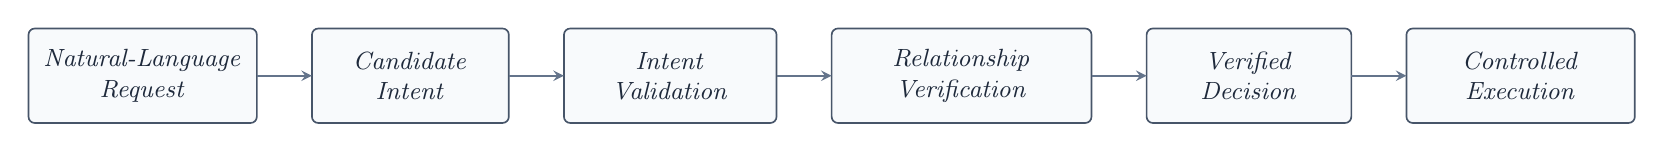
\begin{tikzpicture}[x=1cm,y=1cm,>=stealth]

% ------------------------------------------------------------
% Colours — neutral / non-colorful
% ------------------------------------------------------------
\definecolor{stepfill}{HTML}{F8FAFC}
\definecolor{stepborder}{HTML}{475569}
\definecolor{arrowcol}{HTML}{64748B}
\definecolor{steptext}{HTML}{1E293B}

% ------------------------------------------------------------
% Step 1 — Natural-Language Request
% ------------------------------------------------------------
\draw[
    rounded corners=0.08cm,
    draw=stepborder,
    fill=stepfill,
    line width=0.6pt
]
(0,0) rectangle (2.9,1.2);

\node[
    align=center,
    text=steptext,
    font=\small
] at (1.45,0.6)
{
    \textit{Natural-Language}\\
    \textit{Request}
};

% ------------------------------------------------------------
% Step 2 — Candidate Intent
% ------------------------------------------------------------
\draw[
    rounded corners=0.08cm,
    draw=stepborder,
    fill=stepfill,
    line width=0.6pt
]
(3.6,0) rectangle (6.1,1.2);

\node[
    align=center,
    text=steptext,
    font=\small
] at (4.85,0.6)
{
    \textit{Candidate}\\
    \textit{Intent}
};

% ------------------------------------------------------------
% Step 3 — Intent Validation
% ------------------------------------------------------------
\draw[
    rounded corners=0.08cm,
    draw=stepborder,
    fill=stepfill,
    line width=0.6pt
]
(6.8,0) rectangle (9.5,1.2);

\node[
    align=center,
    text=steptext,
    font=\small
] at (8.15,0.6)
{
    \textit{Intent}\\
    \textit{Validation}
};

% ------------------------------------------------------------
% Step 4 — Relationship Verification
% ------------------------------------------------------------
\draw[
    rounded corners=0.08cm,
    draw=stepborder,
    fill=stepfill,
    line width=0.6pt
]
(10.2,0) rectangle (13.5,1.2);

\node[
    align=center,
    text=steptext,
    font=\small
] at (11.85,0.6)
{
    \textit{Relationship}\\
    \textit{Verification}
};

% ------------------------------------------------------------
% Step 5 — Verified Decision
% ------------------------------------------------------------
\draw[
    rounded corners=0.08cm,
    draw=stepborder,
    fill=stepfill,
    line width=0.6pt
]
(14.2,0) rectangle (16.8,1.2);

\node[
    align=center,
    text=steptext,
    font=\small
] at (15.5,0.6)
{
    \textit{Verified}\\
    \textit{Decision}
};

% ------------------------------------------------------------
% Step 6 — Controlled Execution
% ------------------------------------------------------------
\draw[
    rounded corners=0.08cm,
    draw=stepborder,
    fill=stepfill,
    line width=0.6pt
]
(17.5,0) rectangle (20.4,1.2);

\node[
    align=center,
    text=steptext,
    font=\small
] at (18.95,0.6)
{
    \textit{Controlled}\\
    \textit{Execution}
};

% ------------------------------------------------------------
% Arrows
% ------------------------------------------------------------
\draw[->, line width=0.7pt, draw=arrowcol] (2.9,0.6) -- (3.6,0.6);
\draw[->, line width=0.7pt, draw=arrowcol] (6.1,0.6) -- (6.8,0.6);
\draw[->, line width=0.7pt, draw=arrowcol] (9.5,0.6) -- (10.2,0.6);
\draw[->, line width=0.7pt, draw=arrowcol] (13.5,0.6) -- (14.2,0.6);
\draw[->, line width=0.7pt, draw=arrowcol] (16.8,0.6) -- (17.5,0.6);

\end{tikzpicture}%
}

\caption{Summary of the conceptual workflow of the proposed system.}
\label{fig:concept_summary_flow}
\end{figure}

The following chapter describes how these conceptual elements are realized in
the prototype implementation.

\chapter{Implementation} \label{chap:implementation}

This chapter presents the prototypical implementation of the
graph-based DeFi verification concept developed in
Chapter~\ref{chap:concept}. It describes the technologies and
implementation decisions used to realize the proposed architecture,
with particular attention to structured intent processing,
authoritative knowledge acquisition, relationship verification,
and controlled blockchain execution.

The prototype supports Uniswap V3 single-hop ERC-20 swaps and
Aave V3 supply, withdrawal, borrowing, and repayment on Ethereum
Sepolia. The chapter follows the main components of the conceptual
architecture and discusses relevant implementation challenges
and deviations. The correctness, performance, and requirement
fulfilment of the prototype are assessed in
Chapter~\ref{chap:evaluation}.

%############ 4.1  Prototype Overview and Technology Choices  #######
\section{Prototype Overview and Technology Choices}
\label{sec:prototype_overview}

The prototype implements the four main responsibilities
introduced in Section~\ref{sec:overall_system_concept}:
AI-based intent processing, verification knowledge,
relationship verification, and controlled execution.
These responsibilities are realized through a browser-based
demonstration interface, a Python backend, a Neo4j property
graph, and a separate Node.js execution component.
Figure~\ref{fig:prototype_technology_stack} illustrates
the technologies and communication interfaces.

\begin{figure}[htbp]
    \centering
    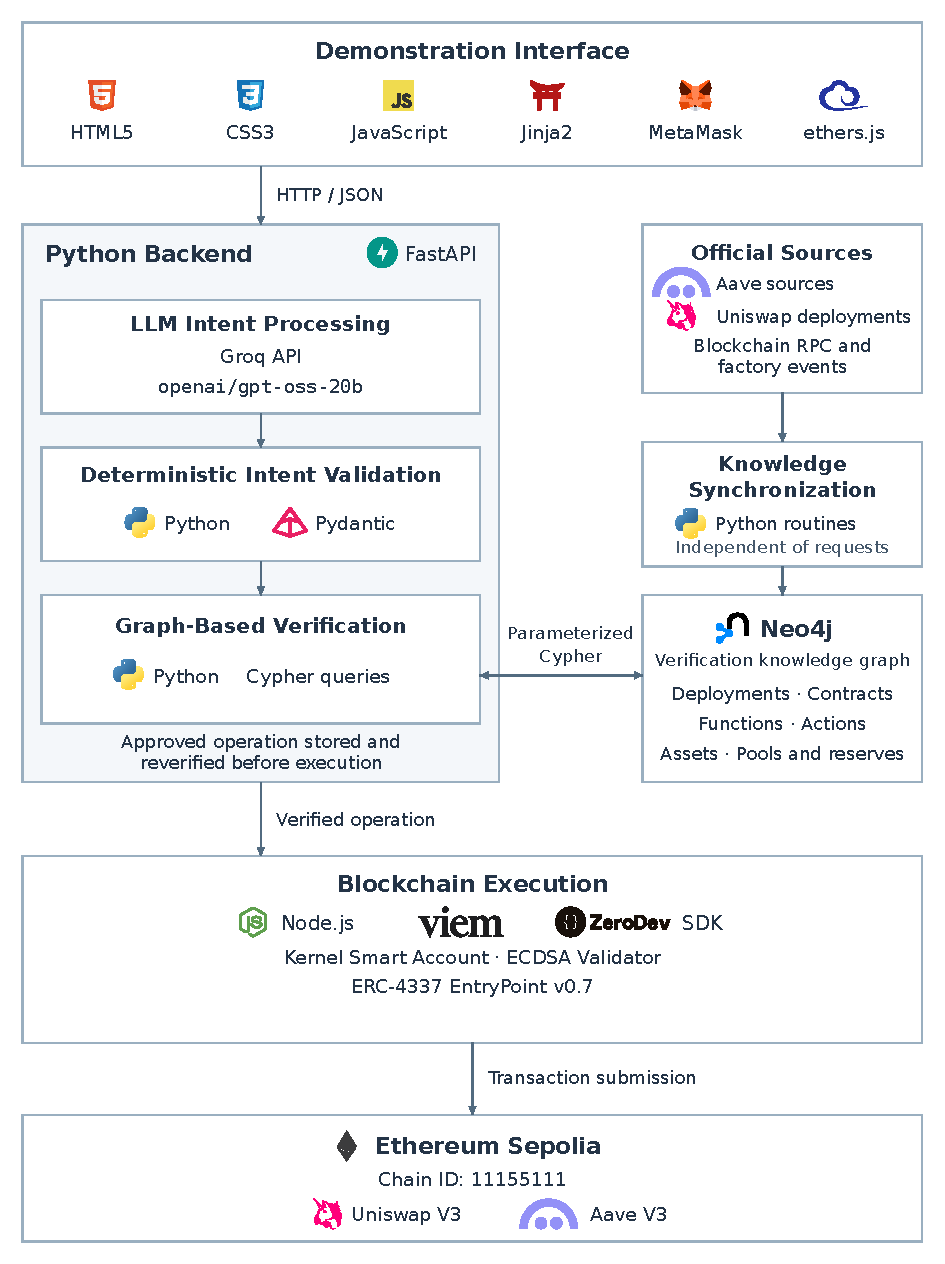
\includegraphics[width=\textwidth]
    {figures/prototype_technology_stack.pdf}
    \caption{Technology stack and communication interfaces
    of the prototype.}
    \label{fig:prototype_technology_stack}
\end{figure}

The demonstration interface is implemented using HTML, CSS,
JavaScript, and Jinja2. It supports natural-language requests,
clarification, verification results, and execution controls.
MetaMask and ethers.js provide browser-wallet connectivity,
while the interface communicates with the backend through
HTTP and JSON. The lightweight design was chosen to keep
the prototype focused on the verification mechanism. The Python backend uses FastAPI and Pydantic to manage API
requests, structured operation models, and the verification
workflow~\cite{implFastAPI,implPydantic}. Intent generation
uses the Groq API with \texttt{openai/gpt-oss-20b}, followed
by deterministic validation. This separation prevents
language-model output from directly determining
execution-critical contract information.

Neo4j was selected because the verification process
requires explicit relationships between protocol
deployments, actions, contracts, functions, and resources.
Parameterized Cypher queries evaluate these connections
against admitted knowledge~\cite{implNeo4jCypher}.
Protocol-specific Python routines acquire and synchronize
this knowledge independently of user requests.

Blockchain interaction is implemented in Node.js using
viem and the ZeroDev SDK. This separates the Python-based
verification logic from the JavaScript smart-account
infrastructure. Execution uses a ZeroDev Kernel smart
account with an ECDSA validator\footnote{In the ZeroDev
Kernel plugin model, a \texttt{sudo} validator provides
unrestricted signing authority, unlike a permission-limited
session-key validator~\cite{implZeroDevPlugins}.}
and ERC-4337 EntryPoint version~0.7
~\cite{implZeroDevSDK,implERC4337}.

Following graph approval, the backend stores the structured
operation and issues an expiring, single-use
\texttt{verification\_id}. Execution retrieves this
operation and repeats graph verification before preparing
the transaction, without reinterpreting the original
request. The implemented authority comparison does not,
however, bind every execution parameter to an immutable
knowledge snapshot. The execution environment is Ethereum Sepolia
(chain ID~11155111). The smart account is controlled by
a backend-configured signer rather than the MetaMask
account connected through the interface. The following
sections describe the implementation of the individual
verification and execution components.


%############ 4.2  LLM-Based Intent Generation  #######

\section{LLM-Based Intent Generation}
\label{sec:llm_intent_generation}

The intent-generation stage implements the language-interpretation
component described in Section~\ref{sec:intent_generation}.
It uses the Groq API with \texttt{openai/gpt-oss-20b} to
convert natural-language requests into candidate structured
intents. The system prompt specifies a JSON representation
containing the action, protocol, input and output assets,
amount, and network. Additional fields capture unsupported
actions, unhandled constraints, and explicitly requested
swap slippage.

The prompt instructs the model to extract information without
introducing assumptions about missing parameters. Unspecified
values are represented as \texttt{null}, while unsupported
operations or conditions should be preserved rather than
silently replaced. For example, ETH must not be substituted
with WETH, and a request mentioning Aave without an action
must not automatically be interpreted as a supply operation.
Contract addresses, functions, and other execution-specific
resources are excluded from the generated intent because
these are resolved through the verification graph. The model is configured with zero temperature, low reasoning
effort, a maximum of 512 completion tokens, and JSON-object
response mode. The latter restricts the response format but
does not enforce a complete intent schema
~\cite{implGroqJSON}. The parser therefore requires a valid
JSON object and retains the expected extraction fields.
Failed model calls or response-parsing attempts are retried
once before an error is returned.

Listing~\ref{lst:generated_intent} illustrates the expected
extraction format for a request to swap 12.375 USDC for WETH
on Uniswap V3 using Ethereum Sepolia with a slippage
tolerance of 0.25\%.

% JSON language definition
\lstdefinelanguage{JSON}{
    morestring=[b]",
    morekeywords={true,false,null},
    sensitive=true,
    showstringspaces=false
}
% Professional JSON listing colors
\definecolor{intentjsonbg}{HTML}{F8FAFC}
\definecolor{intentjsonborder}{HTML}{CBD5E1}
\definecolor{intentjsontext}{HTML}{1E293B}
\definecolor{intentjsonkeyword}{HTML}{1D4ED8}
\definecolor{intentjsonstring}{HTML}{9A3412}
\definecolor{intentjsonnumber}{HTML}{64748B}

% Professional JSON listing style
\lstdefinestyle{intentjson}{
    language=JSON,
    basicstyle=\ttfamily\footnotesize\color{intentjsontext},
    backgroundcolor=\color{intentjsonbg},
    keywordstyle=\color{intentjsonkeyword}\bfseries,
    stringstyle=\color{intentjsonstring},
    numbers=left,
    numberstyle=\ttfamily\tiny\color{intentjsonnumber},
    stepnumber=1,
    numbersep=10pt,
    frame=single,
    framerule=0.5pt,
    rulecolor=\color{intentjsonborder},
    framesep=6pt,
    xleftmargin=2em,
    framexleftmargin=2em,
    xrightmargin=0.5em,
    breaklines=true,
    breakatwhitespace=false,
    columns=fullflexible,
    keepspaces=true,
    showstringspaces=false,
    tabsize=2,
    captionpos=b,
    aboveskip=12pt,
    belowskip=12pt
}

\begin{lstlisting}[
    style=intentjson,
    caption={Illustrative LLM-generated candidate intent for a Uniswap V3 swap.},
    label={lst:generated_intent}
]
{
  "action": "swap",
  "protocol": "Uniswap V3",
  "token_in": "USDC",
  "token_out": "WETH",
  "amount": "12.375",
  "chain": "Ethereum Sepolia",
  "unsupported_action": null,
  "slippage": {
    "value": "0.25",
    "unit": "percent"
  },
  "unhandled_constraints": []
}
\end{lstlisting}


The listing represents the extraction format rather than a
recorded model response. Incomplete requests are processed
using a separate clarification prompt, which receives the
pending candidate, the missing fields, and the user's reply.
The extracted clarification is merged with the existing
candidate and validated again.

The resulting intent remains an untrusted interpretation
of the user's request. Its completeness, supported scope,
and parameter validity are checked by the deterministic
validation component described in
Section~\ref{sec:intent_validation_implementation}.


%############ 4.3  Intent Validation  #######


\section{Intent Validation}
\label{sec:intent_validation_implementation}

The validation stage implements the deterministic checks
described in Section~\ref{sec:intent_validation}. Its main
components are \texttt{llm/normalization.py} and the typed
models in \texttt{core/models.py}. The extracted JSON is
converted into an \texttt{IntentCandidate}, whose fields may
initially be empty to support clarification. Validation
determines whether the candidate represents a complete,
well-formed operation within the supported prototype scope.

Normalization resolves recognized aliases for actions,
protocols, assets, and networks. For example, a deposit
request can be mapped to the Aave supply action. The
supported combinations are Uniswap V3 swaps and Aave V3
supply, withdraw, borrow, and repay operations. Unsupported
actions, protocols, or combinations return
\texttt{UNSUPPORTED} without querying the graph. Amounts are parsed using Python's \texttt{Decimal} type and
must be positive, with no more than 18 fractional decimal
places after removing trailing zeros. Invalid amounts and
swaps with identical normalized input and output assets
produce \texttt{REJECTED}. Recognized Ethereum Sepolia
aliases resolve to chain ID~11155111. An omitted network
uses the configured Sepolia context, whereas an explicitly
different network is unsupported.

For swaps, an explicitly requested slippage tolerance is
converted into basis points\footnote{One basis point (bps)
corresponds to 0.01 percentage points. For example,
100~bps equals 1\%.} and must fall within the supported
range of 1 to 500~bps. When slippage is omitted, the
configured default of 100~bps is applied when preparing
the approved operation. Unsupported conditions, such as
custom recipients, deadlines, and requests containing
multiple operations, prevent further processing rather
than being silently omitted. Additional request-level
checks supplement the model's extraction of such
constraints.

Listing~\ref{lst:required_intent_fields} shows the
action-dependent completeness check implemented in
\texttt{normalization}. Missing information produces
\texttt{NEEDS\_CLARIFICATION} and identifies the fields
required to complete the operation.


% ==================================================
% Professional Python listing style
% ==================================================
\lstdefinestyle{intentpython}{
    language=Python,
    basicstyle=\ttfamily\footnotesize\color{intentjsontext},
    backgroundcolor=\color{intentjsonbg},
    keywordstyle=\color{intentjsonkeyword}\bfseries,
    stringstyle=\color{intentjsonstring},
    commentstyle=\color{intentjsonnumber}\itshape,
    numbers=left,
    numberstyle=\ttfamily\tiny\color{intentjsonnumber},
    stepnumber=1,
    numbersep=10pt,
    frame=single,
    framerule=0.5pt,
    rulecolor=\color{intentjsonborder},
    framesep=6pt,
    xleftmargin=2em,
    framexleftmargin=2em,
    xrightmargin=0.5em,
    breaklines=true,
    breakatwhitespace=false,
    columns=fullflexible,
    keepspaces=true,
    showstringspaces=false,
    tabsize=4,
    captionpos=b,
    aboveskip=12pt,
    belowskip=12pt
}

\begin{lstlisting}[
    style=intentpython,
    caption={Required-field validation and clarification handling.},
    label={lst:required_intent_fields}
]
required = ["action", "protocol", "amount", "token_in"]
if candidate.action == "swap":
    required.append("token_out")

missing = [
    name for name in required
    if getattr(candidate, name) is None
]

if missing:
    friendly = {
        "action": "operation",
        "protocol": "protocol",
        "amount": "amount",
        "token_in": "input asset",
        "token_out": "output asset",
    }

    labels = [friendly[name] for name in missing]

    return IntentResolution(
        status=Decision.NEEDS_CLARIFICATION,
        intent=candidate,
        missing_fields=missing,
        message="Please provide the " + ", ".join(labels) + ".",
        error_code="missing_fields",
    )
\end{lstlisting}


The pending candidate and missing fields are maintained
in process memory by \texttt{pipeline}.
Subsequent clarification responses are merged into the
candidate and validated again. This state has a configurable
expiry but does not survive an application restart.

Successful validation produces an internal
\texttt{APPROVED} status, indicating that the candidate
is ready for graph verification. It does not authorize
execution. Asset symbols are subsequently resolved against
the graph, although the implementation does not explicitly
detect every case of multiple contract addresses sharing
a symbol. Inconsistent capitalization between acquired
Aave symbols and exact-match graph queries may also prevent
a valid asset from being identified. Deterministic
validation therefore establishes structural suitability
without guaranteeing that the extracted intent fully
represents the user's original instruction.


%  #### 4.4 Authoritative Verification Knowledge and Graph Implementation ###

\section{Authoritative Verification Knowledge and Graph Implementation}
\label{sec:verification_knowledge_implementation}

The prototype maintains verification knowledge in a Neo4j
property graph, independently of language-model output and
individual user requests. Protocol-specific acquisition
procedures retrieve deployment and resource information
from external sources, validate the acquired data, and
admit the accepted relationships into the graph. Runtime
verification operates on this maintained representation,
as described in Section~\ref{sec:verification_knowledge}.

\subsection{Knowledge Acquisition and Admission}

The acquisition process distinguishes deployment information,
protocol resources, and callable functions. For Aave V3,
network-specific contract addresses and reserve mappings are
obtained from the official Aave address book
~\cite{implAaveAddressBook}. The acquired information
includes Pool contracts, underlying assets, reserve tokens,
oracles, and interest-rate strategies. Before admission,
the implementation normalizes addresses and checks that
the required contract and asset information is present.

Uniswap V3 deployment information is obtained from the
published deployment records~\cite{implUniswapDeployments}.
The acquisition procedure selects the applicable contracts,
including the factory, swap router, and quoter. It also
queries the blockchain for \texttt{PoolCreated} events,
after checking the RPC network identifier. Event retrieval
is divided into bounded block ranges to accommodate provider
limitations. The resulting records describe pool addresses,
participating tokens, fee tiers, and their creation context.

Discovered pools are not automatically accepted for
verification. The prototype applies a restricted asset
policy under which both pool tokens must belong to an
admitted set consisting of assets represented by active
Aave V3 reserves on the same network and the configured
canonical WETH address. Pools outside this set remain
represented in the graph but are marked as ineligible
for verification. This restriction is a local prototype
policy, not a requirement of the Uniswap protocol.

Callable functions are represented through a configured
interface registry. It associates supported actions with
contract roles, function signatures, and selectors using
the corresponding protocol interfaces
~\cite{implAavePool,implUniswapSingleSwap,implSolidityABI}.
The registry includes Aave lending operations, Uniswap's
\texttt{exactInputSingle} function, and the quoter function
required for swap preparation. Unlike deployment and
resource information, these function mappings are
maintained manually.

\subsection{Implemented Property-Graph Structure}

The graph distinguishes protocol families from their
network-specific deployments. Each deployment is associated
with a \texttt{Chain}, while contracts and tokens are
identified using their network and normalized address.
Selected identifiers are protected by uniqueness constraints,
and Cypher \texttt{MERGE} operations reuse existing graph
entities during synchronization~\cite{implNeo4jCypher}.


Uniswap V3 extends this structure with pools, tokens,
and fee tiers. A deployment connects to its pools through
\texttt{HAS\_POOL}, while \texttt{CREATED\_POOL} records
their factory origin. Token relationships identify the
pool endpoints and participating assets, and fee-tier
relationships preserve the pool configuration.
Figure~\ref{fig:uniswap_graph_implementation}
illustrates a selected subgraph from the implemented
Uniswap V3 verification knowledge. It shows concrete
relationships represented in Neo4j rather than a
complete graph schema. A more detailed reconstruction
of the retrieved graph instance is provided in
Figure~\ref{fig:appendix_uniswap_neo4j}.


\begin{figure}[H]
    \centering
    \resizebox{\linewidth}{!}{%
        

\begingroup
\definecolor{stepfill}{HTML}{F8FAFC}
\definecolor{stepborder}{HTML}{475569}
\definecolor{arrowcol}{HTML}{64748B}
\definecolor{steptext}{HTML}{1E293B}

\begin{tikzpicture}[
    >=stealth,
    graphnode/.style={
        draw=stepborder,
        fill=stepfill,
        text=steptext,
        rounded corners=2pt,
        line width=0.65pt,
        text width=2.67cm,
        minimum height=1.15cm,
        inner xsep=5pt,
        inner ysep=6pt,
        outer sep=0pt,
        align=center,
        font=\sffamily\fontsize{9}{11}\selectfont
    },
    edge/.style={
        ->,
        draw=arrowcol,
        line width=0.76pt,
        rounded corners=0pt,
        shorten <=1pt,
        shorten >=2pt
    },
    rel/.style={
        fill=white,
        text=steptext,
        inner xsep=3pt,
        inner ysep=1.5pt,
        align=center,
        font=\ttfamily\fontsize{7.6}{8.9}\selectfont
    }
]

% --- Top row -----------------------------------------------------
\node[graphnode] (family) at (-5.45,0)
    {\textbf{ProtocolFamily}\\Uniswap V3};
\node[graphnode, text width=3.06cm] (chain) at (5.45,0)
    {\textbf{Chain}\\Ethereum Sepolia\\{\footnotesize chain ID: 11155111}};

% --- Deployment --------------------------------------------------
\node[graphnode, text width=3.72cm] (deployment) at (0,-2.55)
    {\textbf{ProtocolDeployment}\\Uniswap V3 deployment};

% --- Contract layer ---------------------------------------------
\node[graphnode] (router) at (-5.45,-5.0)
    {\textbf{Contract}\\SwapRouter02\\{\footnotesize role: swap\_router}};
\node[graphnode] (factory) at (0,-5.0)
    {\textbf{Contract}\\Uniswap V3 Factory\\{\footnotesize role: factory}};
\node[graphnode] (quoter) at (5.45,-5.0)
    {\textbf{Contract}\\Quoter V2\\{\footnotesize role: quoter}};

% --- Function and pool layer ------------------------------------
\node[graphnode, text width=3.12cm] (execute) at (-5.45,-8.05)
    {\textbf{Function}\\\texttt{exactInputSingle}\\{\footnotesize purpose: execute}\\{\footnotesize selector: \texttt{0x04e45aaf}}};
\node[graphnode] (pool) at (0,-8.05)
    {\textbf{Pool}\\Uniswap V3 pool};
\node[graphnode, text width=4.04cm] (quote) at (5.45,-8.05)
    {\textbf{Function}\\\texttt{quoteExactInputSingle}\\{\footnotesize purpose: preflight}};

% --- Pool resources ---------------------------------------------
\node[graphnode] (token0) at (-2.35,-10.87)
    {\textbf{Token(USDC)}\\Pool token 0 \\{\footnotesize chain ID + address}};
\node[graphnode] (token1) at (2.35,-10.87)
    {\textbf{Token(WETH)}\\Pool token 1 \\{\footnotesize chain ID + address}};

% --- Terminal nodes ---------------------------------------------
\node[graphnode] (action) at (-5.45,-13.45)
    {\textbf{Action}\\\texttt{swap}};
\node[graphnode] (fee) at (0,-13.45)
    {\textbf{FeeTier}\\Pool fee\\configuration};

% --- Top relationships: mirrored orthogonal bends --------------
\draw[edge]
    (family.south) -- (-5.45,-1.36)
    -- node[rel, above, pos=0.50] {HAS\_DEPLOYMENT} (-1.20,-1.36)
    -- ([xshift=-1.20cm]deployment.north);
\draw[edge]
    (chain.south) -- (5.45,-1.36)
    -- node[rel, above, pos=0.50] {HOSTS} (1.20,-1.36)
    -- ([xshift=1.20cm]deployment.north);

% --- Contract ownership: mirrored routing lanes ----------------
\draw[edge]
    ([xshift=-1.47cm]deployment.south) -- (-1.47,-3.58)
    -- node[rel, above, pos=0.51] {DEPLOYED\_CONTRACT} (-5.45,-3.58)
    -- (router.north);
\draw[edge]
    (deployment.south) -- node[rel, left, pos=0.78]
    {DEPLOYED\_CONTRACT} (factory.north);
\draw[edge]
    ([xshift=1.47cm]deployment.south) -- (1.47,-3.58)
    -- node[rel, above, pos=0.49] {DEPLOYED\_CONTRACT} (5.45,-3.58)
    -- (quoter.north);

% --- Pool ownership: dedicated inter-column corridor -----------
\draw[edge]
    ([xshift=0.83cm]deployment.south) -- (0.83,-4.02)
    -- (2.95,-4.02)
    -- node[rel, left, pos=0.54] {HAS\_POOL} (2.95,-8.05)
    -- (pool.east);

% --- Direct contract/function and factory/pool connections ------
\draw[edge]
    (router.south) -- node[rel, left, pos=0.50]
    {EXPOSES\_FUNCTION} (execute.north);
\draw[edge]
    (factory.south) -- node[rel, left, pos=0.50]
    {CREATED\_POOL} (pool.north);
\draw[edge]
    (quoter.south) -- node[rel, right, pos=0.50]
    {EXPOSES\_FUNCTION} (quote.north);

% --- Resource relationships: symmetrical orthogonal bends ------
\draw[edge]
    ([xshift=-0.76cm]pool.south) -- (-0.76,-9.53)
    -- (-2.35,-9.53)
    -- node[rel, left, pos=0.52] {TOKEN0\\SUPPORTS\_TOKEN}
       (token0.north);
\draw[edge]
    ([xshift=0.76cm]pool.south) -- (0.76,-9.53)
    -- (2.35,-9.53)
    -- node[rel, right, pos=0.52] {TOKEN1\\SUPPORTS\_TOKEN}
       (token1.north);
\draw[edge]
    (pool.south) -- node[rel, right, pos=0.77]
    {USES\_FEE\_TIER} (fee.north);

% --- Action relationships: own channels, no node crossings ------
\draw[edge]
    (execute.south) -- node[rel, left, pos=0.58]
    {IMPLEMENTS\_ACTION} (action.north);

\draw[edge]
    (deployment.west) -- node[rel, above, pos=0.47]
    {SUPPORTS\_ACTION} (-8.18,-2.55)
    -- (-8.18,-13.45)
    -- (action.west);

\draw[edge]
    (quote.east) -- (8.22,-8.05)
    -- (8.22,-14.80)
    -- node[rel, above, pos=0.38] {IMPLEMENTS\_ACTION} (-5.45,-14.80)
    -- (action.south);

\end{tikzpicture}
\endgroup
%
    }
    \caption{Selected relationships in the implemented
    Uniswap V3 graph.}
    \label{fig:uniswap_graph_implementation}
\end{figure}

For Aave V3, each lending resource is represented as a
\texttt{Reserve} connected to its deployment through
\texttt{HAS\_RESERVE} and to its underlying asset through
\texttt{UNDERLYING\_ASSET}. Reserve-specific
\texttt{SUPPORTS\_ACTION} relationships describe the
represented lending operations. Additional connections
retain reserve-token, oracle, and interest-rate-strategy
information where available. 
Figure~\ref{fig:aave_graph_implementation}
illustrates the corresponding relationships for
an Aave V3 USDC supply operation. A detailed
reconstruction of the selected graph instance
is provided in Figure~\ref{fig:appendix_aave_neo4j}.


\begin{figure}[H]
    \centering
    \resizebox{\linewidth}{!}{%
        \begingroup
\definecolor{stepfill}{HTML}{F8FAFC}
\definecolor{stepborder}{HTML}{475569}
\definecolor{arrowcol}{HTML}{64748B}
\definecolor{steptext}{HTML}{1E293B}

\begin{tikzpicture}[
  >=stealth,
  graphnode/.style={
    draw=stepborder,
    fill=stepfill,
    text=steptext,
    rounded corners=2pt,
    line width=0.65pt,
    text width=2.78cm,
    minimum height=1.12cm,
    inner xsep=5pt,
    inner ysep=6pt,
    outer sep=0pt,
    align=center,
    font=\sffamily\fontsize{9.4}{11.4}\selectfont
  },
  edge/.style={
    ->,
    draw=arrowcol,
    line width=0.74pt,
    shorten <=1pt,
    shorten >=2pt
  },
  contextedge/.style={
    edge,
    densely dashed
  },
  rel/.style={
    fill=white,
    text=steptext,
    align=center,
    inner xsep=2.5pt,
    inner ysep=1.7pt,
    font=\ttfamily\fontsize{7.7}{9.0}\selectfont
  }
]

% --------------------------------------------------
% Nodes
% --------------------------------------------------

\node[graphnode] (family) at (-5.70,0)
  {\textbf{ProtocolFamily}\\Aave V3};

\node[graphnode,text width=3.00cm] (chain) at (5.70,0)
  {\textbf{Chain}\\Ethereum Sepolia\\
   {\footnotesize chain ID: 11155111}};

\node[graphnode,text width=3.85cm] (deployment)
  at (0,-2.60)
  {\textbf{ProtocolDeployment}\\Aave V3 deployment};

\node[graphnode] (reserve) at (-5.70,-5.35)
  {\textbf{Reserve}\\USDC reserve};

\node[graphnode] (pool) at (5.70,-5.35)
  {\textbf{Contract}\\Aave Pool\\
   {\footnotesize role: pool}};

\node[graphnode] (token) at (-5.70,-8.62)
  {\textbf{Token}\\USDC\\
   {\footnotesize underlying asset}};

\node[graphnode] (action) at (0,-8.62)
  {\textbf{Action}\\\texttt{supply}};

\node[graphnode,text width=3.20cm] (fn)
  at (5.70,-8.62)
  {\textbf{Function}\\\texttt{supply}\\
   {\footnotesize purpose: execute}\\
   {\footnotesize selector: \texttt{0x617ba037}}};

\node[graphnode] (atoken) at (-5.70,-11.85)
  {\textbf{Contract}\\USDC aToken};

\node[graphnode] (debt) at (0,-11.85)
  {\textbf{Contract}\\USDC\\
   {\footnotesize variable-debt token}};

% --------------------------------------------------
% Protocol and chain relationships
% --------------------------------------------------

\draw[edge]
  (family.south) -- (-5.70,-1.42)
  -- node[rel,above,pos=0.49]
     {HAS\_DEPLOYMENT} (-1.15,-1.42)
  -- ([xshift=-1.15cm]deployment.north);

\draw[edge]
  (chain.south) -- (5.70,-1.42)
  -- node[rel,above,pos=0.49]
     {HOSTS} (1.15,-1.42)
  -- ([xshift=1.15cm]deployment.north);

% --------------------------------------------------
% Deployment relationships
% --------------------------------------------------

\draw[edge]
  ([xshift=-1.40cm]deployment.south)
  -- (-1.40,-4.03)
  -- node[rel,above,pos=0.50]
     {HAS\_RESERVE} (-5.70,-4.03)
  -- (reserve.north);

\draw[edge]
  ([xshift=1.40cm]deployment.south)
  -- (1.40,-4.03)
  -- node[rel,above,pos=0.50]
     {DEPLOYED\_CONTRACT} (5.70,-4.03)
  -- (pool.north);

\draw[edge]
  (deployment.south)
  -- node[rel,right,pos=0.58]
     {SUPPORTS\_ACTION}
  (action.north);

% --------------------------------------------------
% Reserve and action relationships
% --------------------------------------------------

\draw[edge]
  (reserve.south)
  -- node[rel,right,pos=0.54]
     {UNDERLYING\_\\ASSET}
  (token.north);

\draw[edge]
  (reserve.east)
  -- (-2.65,-5.35)
  -- node[rel,right,pos=0.50]
     {SUPPORTS\_ACTION} (-2.65,-8.62)
  -- (action.west);

% --------------------------------------------------
% Contract and function relationships
% --------------------------------------------------

\draw[edge]
  (pool.south)
  -- node[rel,right,pos=0.53]
     {EXPOSES\_FUNCTION}
  (fn.north);

\draw[edge]
  (fn.west)
  -- node[rel,above,pos=0.49]
     {IMPLEMENTS\_\\ACTION}
  (action.east);

% --------------------------------------------------
% Supplementary reserve-token relationships
% Dashed edges distinguish contextual graph knowledge.
% --------------------------------------------------

% Reserve -> aToken
\draw[contextedge]
    ([yshift=-4pt]reserve.west)
    -| (-8.12,-11.85)
    -- (atoken.west);

\node[rel, rotate=90]
    at (-8.12,-8.55)
    {HAS\_A\_TOKEN};

% Reserve -> variable-debt token
\draw[contextedge]
    ([yshift=4pt]reserve.west)
    -| (-9.05,-13.28)
    -- node[rel,above,pos=0.46]
       {HAS\_VARIABLE\_DEBT\_TOKEN}
       (0,-13.28)
    -- (debt.south);

% aToken -> underlying asset
\draw[contextedge]
  (atoken.north)
  -- node[rel,right,pos=0.53]
     {REPRESENTS\_\\ASSET}
  (token.south);

% Variable-debt token -> underlying asset
\draw[contextedge]
  (debt.west)
  -- node[rel,above,pos=0.50]
     {DEBT\_FOR} (-3.33,-11.85)
  -- (-3.33,-8.62)
  -- (token.east);

\end{tikzpicture}
\endgroup
%
    }
    \caption{Selected relationships in the implemented
    Aave V3 graph for USDC supply.}
    \label{fig:aave_graph_implementation}
\end{figure}




% ==================================================
% Cypher language definition
% ==================================================
\lstdefinelanguage{Cypher}{
    morekeywords={
        MATCH,OPTIONAL,WHERE,WITH,RETURN,AS,
        AND,OR,NOT,ORDER,BY,LIMIT,MERGE,
        SET,CREATE,DELETE,DETACH,DISTINCT,
        UNWIND,CALL,YIELD,REMOVE,ON,
        CASE,WHEN,THEN,ELSE,END,IN
    },
    sensitive=false,
    morecomment=[l]{//},
    morestring=[b]',
    morestring=[b]"
}

% ==================================================
% Professional Cypher listing colors
% ==================================================
\definecolor{cypherbg}{HTML}{F8FAFC}
\definecolor{cypherborder}{HTML}{CBD5E1}
\definecolor{cyphertext}{HTML}{1E293B}
\definecolor{cypherkeyword}{HTML}{1D4ED8}
\definecolor{cypherstring}{HTML}{9A3412}
\definecolor{cypherlineno}{HTML}{64748B}

% ==================================================
% Professional Cypher listing style
% ==================================================
\lstdefinestyle{thesiscypher}{
    language=Cypher,
    basicstyle=\ttfamily\footnotesize\color{cyphertext},
    backgroundcolor=\color{cypherbg},
    keywordstyle=\color{cypherkeyword}\bfseries,
    stringstyle=\color{cypherstring},
    commentstyle=\color{cypherlineno}\itshape,
    numbers=left,
    numberstyle=\ttfamily\tiny\color{cypherlineno},
    stepnumber=1,
    numbersep=10pt,
    frame=single,
    framerule=0.5pt,
    rulecolor=\color{cypherborder},
    framesep=6pt,
    xleftmargin=2em,
    framexleftmargin=2em,
    xrightmargin=0.5em,
    breaklines=true,
    columns=fullflexible,
    keepspaces=true,
    showstringspaces=false,
    captionpos=b
}

\begin{lstlisting}[
    style=thesiscypher,
    caption={Selected Cypher statements for protocol deployment construction (abridged).},
    label={lst:deployment_graph_construction}
]
MERGE (chain:Chain {chain_id: $chain_id})
MERGE (family:ProtocolFamily {key: $protocol_key})
MERGE (deployment:ProtocolDeployment {key: $deployment_key})

SET deployment.chain_id = $chain_id,
    deployment.source_url = $source_url,
    deployment.graph_version = $graph_version,
    deployment.last_synced_at = $synced_at

MERGE (family)-[:HAS_DEPLOYMENT]->(deployment)
MERGE (chain)-[:HOSTS]->(deployment)
MERGE (deployment)-[:DEPLOYED_ON]->(chain)
\end{lstlisting}


Listing~\ref{lst:deployment_graph_construction}
illustrates how protocol deployments are connected to
their protocol families and blockchain networks.
Source references and synchronization timestamps
are retained as deployment properties.


The shared execution structure connects a deployment to
its supported actions through \texttt{SUPPORTS\_ACTION}
and to its contracts through \texttt{DEPLOYED\_CONTRACT}.
Contracts expose callable functions through
\texttt{EXPOSES\_FUNCTION}, while
\texttt{IMPLEMENTS\_ACTION} identifies the action
associated with each function. Contract roles and active
states are retained on the relevant relationships.

These protocol-specific structures preserve the relationships
needed to establish execution context. The figures present
selected stored relationships; the action-specific Cypher
queries in the following section determine which of these
relationships participate in verification.
Listing~\ref{lst:deployment_graph_construction}
illustrates the construction of a protocol deployment
and its relationship to the corresponding protocol
family and blockchain network. Source references and
synchronization timestamps are stored as properties
of the deployment.

\subsection{Synchronization, Freshness, and Implementation Limits}

Knowledge synchronization follows three stages:
acquisition, validation, and admission. Each protocol
deployment can be synchronized independently through
a command-line workflow. The source information is
retrieved and validated before existing deployment
relationships are updated. This prevents failed acquisition
from immediately replacing previously admitted knowledge. Synchronization outcomes are recorded through
\texttt{KnowledgeSource} nodes and
\texttt{SYNCHRONIZED\_FROM} relationships. The stored
information includes source references, synchronization
status, timestamps, and failure details. During successful
admission, applicable existing relationships are marked
inactive and those present in the accepted data are
reactivated. Historical graph entities can therefore
remain available without necessarily supporting new
verification approvals.

The verifier evaluates knowledge freshness using the most
recent successful synchronization timestamp, with a
configurable maximum age of 168 hours by default.
Unsuccessful synchronization attempts do not automatically
invalidate previously accepted information while that
information remains within the permitted age. Coverage
properties, including \texttt{pool\_discovery\_complete}
and \texttt{asset\_coverage}, indicate the scope of the
acquired data. They do not establish complete knowledge
of all protocol resources.

The synchronization process is invoked explicitly and
does not include a background scheduler or automatic
source-change monitoring. Furthermore, graph admission
consists of multiple database operations rather than
an atomic replacement of the entire deployment. A failure
during admission or a concurrent verification request
can therefore encounter a partially updated graph. Additional limitations concern the admission policies.
Uniswap pool eligibility depends partly on Aave reserve
information already stored in the graph, without an
independent freshness check of that dependency during
admission. For Aave, supply and withdrawal relationships
are inferred from parsed reserves, while borrowing and
repayment relationships depend on the presence of a
variable-debt token. The loader does not examine live
pause, freeze, or borrowing-enabled settings, and obsolete
reserve-action relationships are not comprehensively
removed.

Consequently, the graph represents admitted execution
relationships and their synchronization context, but
does not establish every aspect of current protocol
availability. It also does not preserve an immutable
knowledge snapshot for each verification. These limits
are considered when interpreting the verification
decisions described in the following section.


% ## 4.5 Relationship Verification and Decision  ##

\section{Relationship Verification and Decision}
\label{sec:relationship_verification_implementation}

The verifier implements the action-specific relationship checks
defined in Section~\ref{sec:relationship_verification} through
parameterized Cypher queries. It receives the normalized protocol,
action, assets, and chain identifier. The amount and slippage
parameters are retained for execution preparation but do not
participate in the graph queries. Verification is performed against
the admitted knowledge described in
Section~\ref{sec:verification_knowledge_implementation}.

\subsection{Action-Specific Relationship Verification}

% For Uniswap V3, the verifier requires a deployment that supports
% the swap action, an active and verification-eligible liquidity pool
% connecting the requested assets, and verified router and quoter
% contracts exposing the corresponding functions. All components
% must belong to the applicable deployment and network context.

% Listing~\ref{lst:uniswap_verification_query} presents the
% implemented relationship query. Rather than checking the
% existence of individual contracts or tokens independently,
% the query matches their required connections within the
% same deployment.

% \begin{lstlisting}[
%     style=thesiscypher,
%     caption={Parameterized relationship verification for a Uniswap V3 swap.},
%     label={lst:uniswap_verification_query}
% ]
% MATCH (family:ProtocolFamily)-[:HAS_DEPLOYMENT]->
%       (deployment:ProtocolDeployment {verified:true, chain_id:$chain_id})
% WHERE toLower(family.name) = toLower($protocol)
% MATCH (deployment)-[:SUPPORTS_ACTION]->(action:Action {name:'swap'})
% MATCH (deployment)-[pool_rel:HAS_POOL]->
%       (pool:Pool {verified:true, verification_eligible:true, active:true, chain_id:$chain_id})
% MATCH (pool)-[:SUPPORTS_TOKEN]->
%       (t1:Token {symbol:$token_in, verified:true, verification_eligible:true, chain_id:$chain_id})
% MATCH (pool)-[:SUPPORTS_TOKEN]->
%       (t2:Token {symbol:$token_out, verified:true, verification_eligible:true, chain_id:$chain_id})
% MATCH (deployment)-[router_rel:DEPLOYED_CONTRACT {role:'swap_router'}]->
%       (router:Contract {verified:true})-[:EXPOSES_FUNCTION]->
%       (fn:Function {verified:true, purpose:'execute'})-[:IMPLEMENTS_ACTION]->(action)
% MATCH (deployment)-[quoter_rel:DEPLOYED_CONTRACT {role:'quoter'}]->
%       (quoter:Contract {verified:true})-[:EXPOSES_FUNCTION]->
%       (:Function {verified:true, purpose:'preflight'})-[:IMPLEMENTS_ACTION]->(action)
% WHERE pool_rel.active=true AND router_rel.active=true AND quoter_rel.active=true
%   AND t1.address <> t2.address
%   AND t1.decimals IS NOT NULL AND t2.decimals IS NOT NULL AND pool.fee IS NOT NULL
% RETURN router.address AS address, quoter.address AS quoter_address,
%        pool.address AS pool_address, pool.fee AS pool_fee,
%        coalesce(pool.featured, false) AS featured,
%        t1.address AS token_in_address, t1.symbol AS token_in_symbol,
%        t1.decimals AS token_in_decimals,
%        t2.address AS token_out_address, t2.symbol AS token_out_symbol,
%        t2.decimals AS token_out_decimals,
%        fn.name AS function_name, fn.signature AS function_signature,
%        fn.selector AS function_selector,
%        family.name AS protocol, $chain_id AS chain_id
% ORDER BY featured DESC, pool.fee ASC, pool.address ASC
% LIMIT 20
% \end{lstlisting}

% The query returns graph-derived contract addresses, function
% information, pool fees, and token decimals. Matching routes
% are ordered by their recorded featured status, fee tier, and
% pool address, with a maximum of 20 results. This ordering
% does not represent price optimization. A matching path
% establishes structural compatibility with the stored
% knowledge but does not establish current liquidity or
% guarantee that the requested swap can be executed.

% Aave V3 uses a different relationship pattern because lending
% operations depend on reserves rather than liquidity pools.
% The verifier checks whether the deployment and the relevant
% reserve support the requested action. The reserve must
% reference the requested underlying asset, while the
% deployment's Pool contract must expose a function
% implementing the same action.

% Listing~\ref{lst:aave_verification_query} shows the
% corresponding query for supply, withdraw, borrow, and repay.

% \begin{lstlisting}[
%     style=thesiscypher,
%     caption={Parameterized reserve and function verification for Aave V3.},
%     label={lst:aave_verification_query}
% ]
% MATCH (family:ProtocolFamily)-[:HAS_DEPLOYMENT]->
%       (deployment:ProtocolDeployment {verified:true, chain_id:$chain_id})
% WHERE toLower(family.name) = toLower($protocol)
% MATCH (deployment)-[:SUPPORTS_ACTION]->(action:Action {name:$action})
% MATCH (deployment)-[reserve_rel:HAS_RESERVE]->
%       (reserve:Reserve {verified:true, active:true})
% MATCH (reserve)-[:UNDERLYING_ASSET]->
%       (token:Token {symbol:$token_in, chain_id:$chain_id, verified:true})
% MATCH (reserve)-[:SUPPORTS_ACTION]->(action)
% MATCH (deployment)-[pool_rel:DEPLOYED_CONTRACT {role:'pool'}]->
%       (pool:Contract {verified:true})-[:EXPOSES_FUNCTION]->
%       (fn:Function {verified:true, purpose:'execute'})-[:IMPLEMENTS_ACTION]->(action)
% WHERE reserve_rel.active=true AND pool_rel.active=true
% RETURN pool.address AS address, null AS pool_address,
%        token.address AS token_address, token.decimals AS token_decimals,
%        fn.name AS function_name, fn.signature AS function_signature,
%        fn.selector AS function_selector,
%        family.name AS protocol, $chain_id AS chain_id
% LIMIT 1
% \end{lstlisting}

% The returned contract, asset, and function information is
% used for subsequent transaction preparation. Unlike the
% Uniswap query, this pattern verifies an action-specific
% reserve relationship. It does not establish the user's
% available collateral, outstanding debt, health factor,
% or the feasibility of the requested lending operation.

For Uniswap V3, the verifier requires a deployment
supporting the swap action, an active and eligible
liquidity pool connecting the requested assets, and
verified router and quoter contracts exposing the
corresponding functions. These relationships must
match within the same deployment and network context.
The query returns contract addresses, function
information, pool fees, and token properties required
for execution preparation. Matching routes are ordered
by their recorded attributes rather than quoted prices.

Aave V3 follows a different relationship pattern because
lending operations depend on reserves rather than
liquidity pools. The verifier requires an active reserve
linked to the requested underlying asset, action support
from both the reserve and deployment, and a verified Pool
contract exposing the corresponding lending function.
The query returns the contract, asset, and function
information required for transaction preparation.

In both cases, verification checks connected relationships
rather than the independent existence of contracts and
assets. The complete parameterized Cypher queries are
provided in Appendix~\ref{app:runtime_verification_queries}.

Although both protocols use the same verification pipeline,
their implementations differ in knowledge acquisition,
graph relationships, and transaction preparation.
Table~\ref{tab:protocol_implementation_differences}
summarizes these differences and the components that
would need adaptation when supporting additional protocols.

\begin{table}[htbp]
\centering
\begingroup
\small
\renewcommand{\arraystretch}{1.18}
\caption{Protocol-specific implementation differences.}
\label{tab:protocol_implementation_differences}

\begin{tabular}{
    @{}
    p{0.21\linewidth}
    p{0.33\linewidth}
    p{0.33\linewidth}
    @{}
}
\hline
\textbf{Aspect} &
\textbf{Uniswap V3} &
\textbf{Aave V3} \\
\hline

Supported actions &
Swap &
Supply, withdraw, borrow, repay \\

Main resource &
Liquidity pool &
Lending reserve \\

Execution contracts &
SwapRouter02 and Quoter V2 &
Aave Pool \\

Required relationships &
Deployment, action, pool, assets, router, quoter,
and callable functions &
Deployment, action, reserve, underlying asset,
Pool contract, and callable function \\

Supporting graph data &
Factory origin, token positions, and fee tiers &
aToken and variable-debt token associations \\

Knowledge acquisition &
Deployment records and factory events &
Address-book and reserve information \\

Execution preparation &
Route quotation, slippage, balances,
and token allowances &
Lending calldata, balances, and
action-specific allowances \\

Extension requirements &
Pool discovery, routing, quoting,
and swap interfaces &
Reserve models, lending actions,
and protocol-specific interfaces \\

\hline
\end{tabular}
\endgroup
\end{table}


\subsection{Verification Decisions and Traceability}

Before evaluating the relationship patterns, the verifier
checks the availability and freshness of the applicable
knowledge. The most recent successful synchronization
timestamp is compared with a configurable age limit,
which defaults to 168 hours. Missing deployment information,
stale knowledge, or unavailable graph access prevents
approval and produces \texttt{INSUFFICIENT\_EVIDENCE}. A matching relationship pattern in fresh admitted knowledge
can produce \texttt{APPROVED}. When no matching path exists,
the verifier distinguishes an unsupported relationship
from incomplete knowledge. If the applicable coverage
indicator records sufficient completeness, the result is
\texttt{REJECTED}. Otherwise, the verifier returns
\texttt{INSUFFICIENT\_EVIDENCE}.

For Uniswap, the completeness assessment uses the recorded
pool-discovery indicator. For Aave, it uses the declared
address-book asset coverage. These indicators describe the
scope of locally synchronized knowledge rather than proving
universal protocol completeness. A positive relationship
match does not require exhaustive coverage of all protocol
resources. Requests outside the supported scope return
\texttt{UNSUPPORTED} before relationship matching. The verification result contains the decision, normalized
operation context, and resolved execution information or
an explanatory failure reason. 

Verification latency is
recorded separately from language-model interpretation and
blockchain submission. For unsuccessful outcomes, the implementation can also
produce structured diagnostic information. This includes
rule identifiers, relevant entities or relationships, and
expected and observed conditions where the available
evidence permits localization. Source, freshness, and
coverage information provide context for interpreting
the failure. These diagnostics are constructed through
deterministic checks rather than generated by the language
model.

Diagnostic inspection is bounded and does not necessarily
identify a unique cause. A failure may remain
\texttt{not\_localized}, or diagnostics may be
\texttt{unavailable}. Neither condition changes the
original verification decision.

Figures~\ref{fig:verification_result} and
\ref{fig:verification_rejection} illustrate the approved
and rejected outcomes presented through the prototype
interface.

\begin{figure}[H]
    \centering
    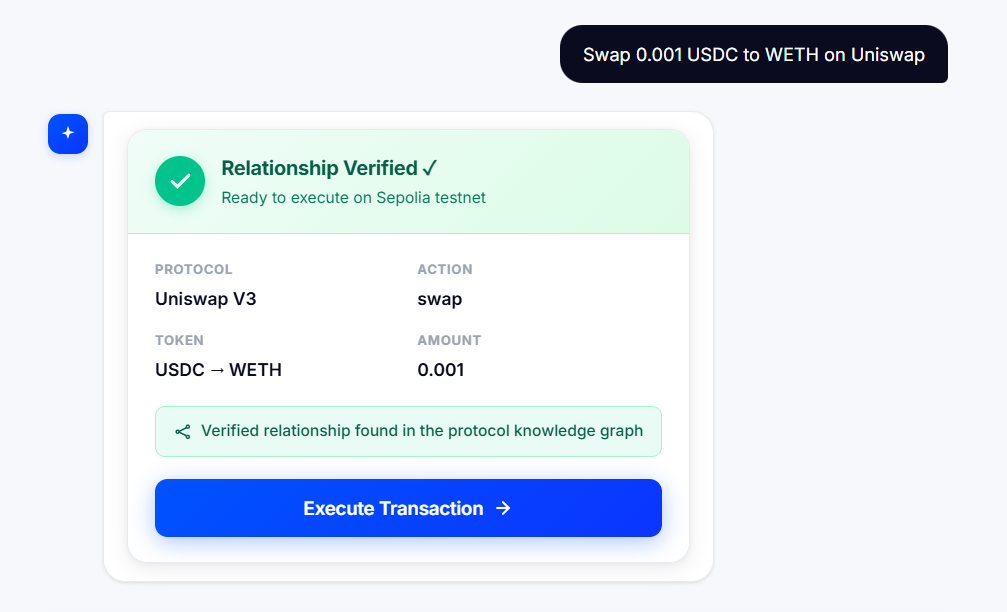
\includegraphics[width=0.90\linewidth]
        {figures/verification_result.png}
    \caption{Approved Uniswap V3 swap displayed before
    blockchain submission.}
    \label{fig:verification_result}
\end{figure}

An approved result establishes consistency with the
represented execution relationships within the admitted
knowledge context. It does not guarantee transaction
success, economic safety, or the absence of smart-contract
vulnerabilities. The returned information also does not
constitute a complete, immutable record of every verified
relationship.
\begin{figure}[H]
    \centering
    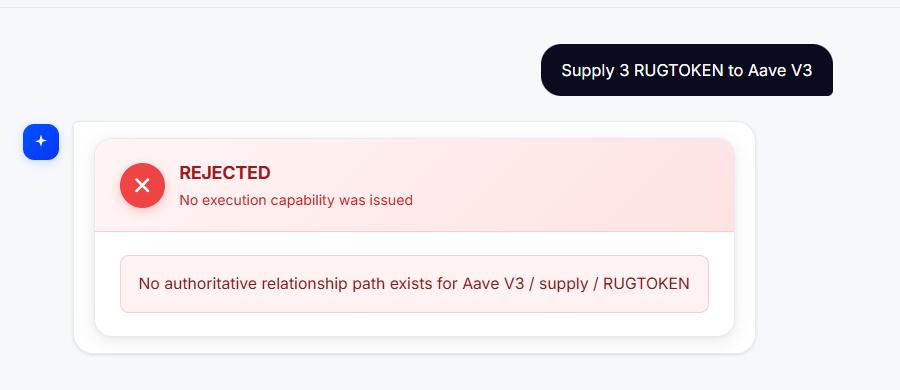
\includegraphics[width=0.85\linewidth]
        {figures/verification_result_failure.png}
    \caption{Rejected Aave V3 supply request for
    \texttt{RUGTOKEN}, without execution authorization.}
    \label{fig:verification_rejection}
\end{figure}


Following approval, the backend retains the structured
operation and creates an expiring verification identifier.
The controlled handover to smart-wallet execution is
described in the following section.


% % #### 4.6 Controlled Smart-Wallet Execution ###
\section{Controlled Smart-Wallet Execution}
\label{sec:controlled_execution_implementation}


After reviewing the approved operation, the user can
initiate execution through the demonstration interface.
This confirmation triggers the execution request but does
not constitute cryptographic authorization by the connected
MetaMask account. 




\begin{figure}[H]
    \centering
    \resizebox{0.95\linewidth}{!}{%
        % \begingroup
% \definecolor{stepfill}{HTML}{F8FAFC}
% \definecolor{stepborder}{HTML}{475569}
% \definecolor{arrowcol}{HTML}{64748B}
% \definecolor{steptext}{HTML}{1E293B}

% \begin{tikzpicture}[
%     >=stealth,
%     execbox/.style={
%         draw=stepborder,
%         fill=stepfill,
%         text=steptext,
%         rounded corners=2pt,
%         line width=0.6pt,
%         text width=6.2cm,
%         minimum height=1.6cm,
%         inner xsep=8pt,
%         inner ysep=6pt,
%         align=center,
%         font=\sffamily\linespread{1}\fontsize{10}{12}\selectfont,
%         execute at begin node={
%             \hyphenpenalty=10000
%             \exhyphenpenalty=10000
%         }
%     },
%     execarrow/.style={
%         ->,
%         draw=arrowcol,
%         line width=0.75pt,
%         shorten <=2pt,
%         shorten >=2pt
%     },
%     execfailure/.style={
%         draw=arrowcol,
%         line width=0.6pt,
%         dashed
%     }
% ]

% \node[execbox] (request) at (0,0)
%     {\textbf{Receive execution request}\\
%      Verification identifier\\
%      Wallet address};

% \node[execbox] (claim) at (0,-2.15)
%     {\textbf{Claim stored approval}\\
%      Check existence, expiry, and reuse\\
%      Retrieve approved operation};

% \node[execbox] (authority) at (0,-4.30)
%     {\textbf{Recheck graph authority}\\
%      Query using saved intent\\
%      Compare approval and current authority};

% \node[execbox] (prepare) at (0,-6.45)
%     {\textbf{Prepare protocol calls}\\
%      Validate parameters and local policy\\
%      Quotes, balances, and allowances};

% \node[execbox] (submit) at (0,-8.60)
%     {\textbf{Submit call batch}\\
%      Kernel smart account\\
%      ZeroDev bundler and paymaster};

% \node[execbox] (result) at (0,-10.75)
%     {\textbf{Return \texttt{EXECUTED}}\\
%      Transaction hash\\
%      Execution summary};

% \node[execbox, text width=2.8cm]
%     (failed) at (7.2,-4.30)
%     {\textbf{Return \texttt{FAILED}}\\
%      Failed check or\\
%      submission error};

% % Main processing path
% \draw[execarrow] (request.south) -- (claim.north);
% \draw[execarrow] (claim.south) -- (authority.north);
% \draw[execarrow] (authority.south) -- (prepare.north);
% \draw[execarrow] (prepare.south) -- (submit.north);
% \draw[execarrow] (submit.south) -- (result.north);

% % Shared failure path
% \draw[execfailure] (4.6,0) -- (4.6,-8.60);

% \draw[execfailure] (request.east) -- (4.6,0);
% \draw[execfailure] (claim.east) -- (4.6,-2.15);
% \draw[execfailure] (authority.east) -- (4.6,-4.30);
% \draw[execfailure] (prepare.east) -- (4.6,-6.45);
% \draw[execfailure] (submit.east) -- (4.6,-8.60);

% \draw[execarrow, dashed]
%     (4.6,-4.30) -- (failed.west);

% \end{tikzpicture}
% \endgroup

\begingroup
\definecolor{stepfill}{HTML}{F8FAFC}
\definecolor{stepborder}{HTML}{475569}
\definecolor{arrowcol}{HTML}{64748B}
\definecolor{steptext}{HTML}{1E293B}

\begin{tikzpicture}[
    >=stealth,
    execbox/.style={
        draw=stepborder,
        fill=stepfill,
        text=steptext,
        rounded corners=2pt,
        line width=0.6pt,
        text width=6.2cm,
        minimum height=1.6cm,
        inner xsep=8pt,
        inner ysep=6pt,
        align=center,
        font=\sffamily\linespread{1}\fontsize{10}{12}\selectfont,
        execute at begin node={
            \hyphenpenalty=10000
            \exhyphenpenalty=10000
        }
    },
    execarrow/.style={
        ->,
        draw=arrowcol,
        line width=0.75pt,
        shorten <=2pt,
        shorten >=2pt
    },
    execfailure/.style={
        draw=arrowcol,
        line width=0.6pt,
        dashed
    }
]

\node[execbox] (approve) at (0,0)
    {\textbf{User confirms approved operation}\\
     Review approved result\\
     Select \textit{Execute Transaction}};

\node[execbox] (request) at (0,-2.15)
    {\textbf{Receive execution request}\\
     Verification identifier\\
     Wallet address};

\node[execbox] (claim) at (0,-4.30)
    {\textbf{Claim stored approval}\\
     Check existence, expiry, and reuse\\
     Retrieve approved operation};

\node[execbox] (authority) at (0,-6.45)
    {\textbf{Recheck graph authority}\\
     Query using saved intent\\
     Compare approval and current authority};

\node[execbox] (prepare) at (0,-8.60)
    {\textbf{Prepare protocol calls}\\
     Check parameters and read-only state\\
     Attest exact batch and expiry};

\node[execbox] (submit) at (0,-10.75)
    {\textbf{Submit call batch}\\
     Restricted Kernel validator\\
     Exact batch, expiry, and one use};

\node[execbox] (result) at (0,-12.90)
    {\textbf{Return \texttt{EXECUTED}}\\
     Successful UserOperation receipt\\
     Execution summary};

\node[execbox, text width=2.8cm]
    (failed) at (7.2,-6.45)
    {\textbf{Return \texttt{FAILED}}\\
     Failed check or\\
     submission error};

% Main processing path
\draw[execarrow] (approve.south) -- (request.north);
\draw[execarrow] (request.south) -- (claim.north);
\draw[execarrow] (claim.south) -- (authority.north);
\draw[execarrow] (authority.south) -- (prepare.north);
\draw[execarrow] (prepare.south) -- (submit.north);
\draw[execarrow] (submit.south) -- (result.north);

% Shared failure path
\draw[execfailure] (4.6,-2.15) -- (4.6,-10.75);

\draw[execfailure] (request.east) -- (4.6,-2.15);
\draw[execfailure] (claim.east) -- (4.6,-4.30);
\draw[execfailure] (authority.east) -- (4.6,-6.45);
\draw[execfailure] (prepare.east) -- (4.6,-8.60);
\draw[execfailure] (submit.east) -- (4.6,-10.75);

\draw[execarrow, dashed]
    (4.6,-6.45) -- (failed.west);

\end{tikzpicture}
\endgroup%
    }
    \caption{Implemented controlled execution workflow after explicit user
confirmation of the approved operation.}
    \label{fig:controlled_execution_flow}
\end{figure}
The execution stage implements the controlled handover
described in Section~\ref{sec:controlled_execution}.
The client submits a verification identifier and wallet
address to \texttt{/api/execute}. The backend retrieves
the approved structured operation from server-side state
rather than reconstructing it from the original
natural-language request. Figure~\ref{fig:controlled_execution_flow}
shows the implemented workflow, including approval retrieval,
validity checks, transaction preparation, and submission.
\subsection{Approval Handover and Validity Checks}

Following successful graph verification, the backend
stores an \texttt{ApprovedOperation} under a randomly
generated \texttt{verification\_id}. The identifier
expires after a configurable period, set to 600 seconds
by default. A lock-protected claim operation retrieves
a copy of the stored approval and consumes the identifier,
preventing its reuse. The client cannot replace the
approved action, assets, amount, or contract information.
An unsuccessful execution attempt therefore requires
a new verification.

Before transaction preparation, the backend repeats
relationship verification using the stored intent.
The renewed result must be approved and retain the
original target contract and function selector.
For Aave operations, the underlying asset address and
decimals must also remain unchanged. For Uniswap swaps,
only originally retained routes that still match the renewed graph result
are passed to preparation. The comparison includes router, pool, fee tier,
assets, quoter, token decimals, function signature, and selector. Network,
protocol, and action must also remain unchanged. A failed comparison
prevents execution.


This mechanism reassesses graph authority without requiring an immutable
knowledge snapshot. The configured development smart account is retained
with the approval. After read-only preparation, the backend independently
checks the complete encoded batch against the retained operation. It then
authorizes those exact bytes; submission neither selects another route nor
recalculates the quote. The wallet authorization expires no later than the
original approval and at most 120 seconds after issuance.


\subsection{Transaction Preparation and Submission}

The backend invokes the Node.js execution component
through a subprocess interface that exchanges structured
JSON data. Blockchain interaction uses viem for contract
reads, amount conversion, and calldata encoding
~\cite{implViem}. The ZeroDev SDK provides a Kernel
3.1 smart account configured with ERC-4337 EntryPoint
version~0.7 on Ethereum Sepolia
~\cite{implZeroDevSDK,implERC4337}. A bundler handles
submission, while a paymaster supports transaction
sponsorship. In the restricted implementation, three signing roles are
separate. The privileged owner installs a custom ERC-7579 secondary
validator, \texttt{GraphBoundValidator}, on a development Kernel account.
A backend graph authority attests the prepared operation after capability
claim and re-verification. A restricted execution key signs the
UserOperation through the SDK's \texttt{regular} plugin. The execution
worker receives neither the owner key nor the authority key and has no
\texttt{sudo} fallback. The connected MetaMask address remains interface
context rather than proof of ownership of the configured smart account.

The validator checks the authority's signature over a commitment to the
complete Kernel execution calldata, account, chain, execution key, validator,
configuration epoch, approval identifier, and validity window. EntryPoint
enforces the returned time bounds. The validator consumes each approval
identifier once and enforces an owner-configured maximum UserOperation gas
cost. Consequently, changing a destination, selector, argument, native value,
or batch member invalidates the authorization. General message-signature
authorization and direct execution through this validator are disabled.
The owner retains installation and revocation authority. Installation
calldata is prepared separately; deployment and installation on Sepolia
were not performed during the supplementary local evaluation.

Before constructing a transaction, the execution
component checks the graph-derived contract addresses,
function signatures and selectors\footnote{A Solidity
function selector consists of the first four bytes
of the function signature's Keccak-256 hash and
identifies the function invoked by the encoded
call data~\cite{implSolidityABI}.}, token decimals,
and action-specific parameters. Amounts are converted
into token base units and checked for positive values.
A local allowlist restricts transaction destinations,
but the normal execution path can add currently
verified destinations to this list. It therefore
does not provide an independent user-defined
authorization policy. The allowlist remains an application-level preflight check. Independent
wallet enforcement is provided by the signed batch commitment and the
one-use validator. Token approvals are limited to the exact operation
amount; a reset to zero may precede them. A cumulative budget across
separately approved operations is not implemented.


Figure~\ref{fig:blockchain_execution} shows the
execution response for a Uniswap V3 swap, including
the transaction hash, smart-account address, and
quoted and minimum output amounts.

\begin{figure}[H]
    \centering
    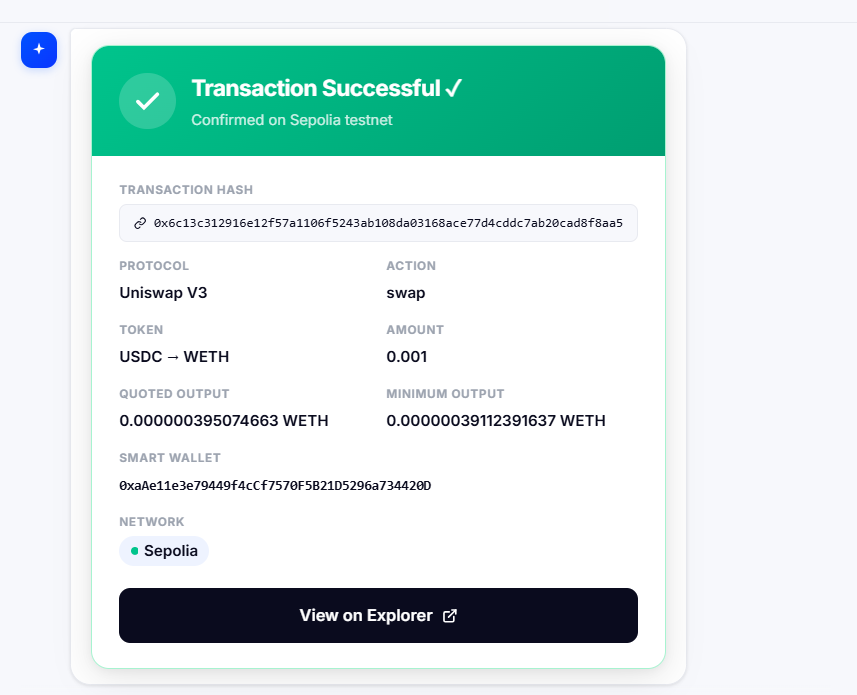
\includegraphics[width=0.95\linewidth]
        {figures/blockchain_execution.png}
    \caption{Transaction submission response for a
    Uniswap V3 swap on Ethereum Sepolia.}
    \label{fig:blockchain_execution}
\end{figure}

For Uniswap V3 swaps, the execution component obtains
quotes for retained routes that still match the renewed graph
verification and selects the route with the highest
positive quoted output. The minimum acceptable output
is calculated using the stored slippage tolerance,
with a default of 100 basis points when no value
was specified. Before invoking
\texttt{exactInputSingle}, the component checks the
smart account's token balance and allowance. Where
necessary, the submitted call batch resets an existing
non-zero allowance and approves the required input
amount~\cite{implUniswapSingleSwap}.

For Aave V3, the execution component prepares supply,
withdraw, borrow, and repay calls using the verified
Pool contract and underlying asset~\cite{implAavePool}.
Borrowing and repayment use variable interest-rate
mode~2, and the referral code defaults to zero.
Supply operations check the available token balance,
while supply and repayment prepare the necessary
allowance changes. Dedicated checks for borrowing
capacity, collateral sufficiency, outstanding debt,
and lending-position constraints are not implemented.
Graph approval therefore does not establish that
the lending transaction will succeed.

The Kernel client submits the authorized calldata and waits for a
successful UserOperation receipt before reporting \texttt{EXECUTED}.
The existing response reason code \texttt{TRANSACTION\_SUBMITTED} is
retained for interface compatibility. A reverted operation, failed
preparation, or submission error produces \texttt{FAILED}.



Receipt waiting does not provide persistent reconciliation, finality
monitoring, or post-execution balance checks. Figure~\ref{fig:blockchain_execution}
records the earlier demonstration and is not evidence of the new validator
on Sepolia. The supplementary authorization evidence is limited to local
contract execution, as described in Chapter~\ref{chap:evaluation}.


% ## 4.7 Summary ###

\section{Summary}
\label{sec:implementation_summary}

The prototype implements the proposed concept through distinct
stages of LLM-based intent generation, deterministic validation,
verification against maintained property-graph knowledge, and
controlled smart-wallet execution. Uniswap V3 swaps and Aave V3
supply, withdrawal, borrowing, and repayment are supported within
the configured Ethereum Sepolia context. Protocol-specific
knowledge acquisition and action-centred Cypher queries separate
language interpretation from the resolution of contracts, functions,
and protocol resources.

The implementation also reveals limitations in realizing the
conceptual guarantees. Knowledge synchronization requires external
invocation and is not fully atomic, while live Aave reserve
restrictions are only partially represented. Verification results
do not retain immutable evidence snapshots. The revised execution
endpoint retains matching routes and binds the prepared batch to a
one-use wallet authorization. The supplementary local tests establish
this enforcement boundary, while Sepolia installation, operational
bundler compatibility, and authentication of the connected browser
account remain outside the demonstrated scope.

The following chapter evaluates intent processing, relationship
verification, knowledge maintenance, and the controlled execution
handover against the defined requirements.



% Thesis Code Listings Configuration

% Colors
\definecolor{thesiscodebg}{HTML}{F8FAFC}
\definecolor{thesiscodeborder}{HTML}{CBD5E1}
\definecolor{thesiscodekw}{HTML}{1D4ED8}
\definecolor{thesiscodecomment}{HTML}{64748B}
\definecolor{thesiscodebrown}{HTML}{B45309}

% General style
\lstdefinestyle{thesiscode}{
    basicstyle=\ttfamily\footnotesize,
    backgroundcolor=\color{thesiscodebg},
    keywordstyle=\color{thesiscodekw}\bfseries,
    commentstyle=\color{thesiscodecomment},
    stringstyle=\color{thesiscodebrown},
    numbers=left,
    numberstyle=\tiny\color{thesiscodecomment},
    numbersep=6pt,
    frame=single,
    rulecolor=\color{thesiscodeborder},
    framerule=0.5pt,
    breaklines=true,
    breakatwhitespace=true,
    columns=fullflexible,
    keepspaces=true,
    showstringspaces=false,
    tabsize=4,
    captionpos=b,
    aboveskip=0.75\baselineskip,
    belowskip=0.8\baselineskip,
    xleftmargin=0.5em,
    xrightmargin=0.5em
}

% JSON language
\lstdefinelanguage{JSON}{
    morestring=[b]",
    morekeywords={true,false,null},
    keywordstyle=\color{thesiscodekw}\bfseries,
    stringstyle=\color{thesiscodebrown},
    sensitive=true
}

% Cypher language
\lstdefinelanguage{Cypher}{
    morekeywords={
        MATCH,WHERE,WITH,RETURN,AS,AND,OR,NOT,
        ORDER,BY,LIMIT,MERGE,SET,CREATE,DELETE,
        DISTINCT,OPTIONAL,TRUE,FALSE,NULL
    },
    sensitive=false,
    morecomment=[l]{//},
    morestring=[b]',
    morestring=[b]"
}

% Apply style
\lstset{style=thesiscode}


\chapter{Evaluation} \label{chap:evaluation}


This chapter evaluates the implemented prototype against the requirements
defined in Section~\ref{sec:requirements_analysis}. The evaluation
examines the correctness of natural-language intent processing,
action-specific relationship verification, and the maintenance of
verification knowledge. It also considers the traceability of
verification decisions, verification latency, and the controlled
handover of approved operations to smart-wallet execution.

The experimental evaluation separates intent processing from graph
verification to assess both stages independently and prevent
interpretation errors from being concealed by an apparently correct
final decision. It also distinguishes graph approval from transaction
preparation and blockchain execution. An approval indicates that the
requested operation is consistent with the admitted verification
knowledge within the supported prototype scope, but does not
guarantee successful execution. The chapter is divided into two parts. The experimental evaluation
presents the evaluation goals, methodology, results, and discussion,
including threats to validity. It examines the individual processing
stages and the complete verification pipeline, together with
knowledge-maintenance scenarios and supplementary execution-control
tests. The requirements evaluation then assesses the fulfilment of
requirements R1 to R6 using the experimental findings and compares the
prototype with the approach groups discussed in the state of the art
analysis.


% ### 5.1 Evaluation Goals ###

\section{Evaluation Goals}
\label{sec:evaluation_goals}

The main goal of the evaluation is to assess whether the implemented
prototype can correctly interpret natural-language DeFi requests and
verify the execution relationships required by the requested operations.
The evaluation focuses on Uniswap V3 swaps and Aave V3 lending operations
on Ethereum Sepolia. It examines the individual processing stages and
their interaction, with particular attention to preventing the approval
of operations that are inconsistent with the admitted verification
knowledge.

The evaluation addresses six research questions derived from the
requirements defined in Section~\ref{sec:requirements_analysis}:

\begin{enumerate}
    \item[\textbf{Q1:}] How accurately does the language model extract
    the requested action, protocol, assets, amount, network, and
    additional constraints, and how reliably do normalization and
    deterministic validation handle incomplete, ambiguous, or
    unsupported requests?

    \item[\textbf{Q2:}] Can graph-based verification correctly distinguish
    valid execution relationships from invalid combinations of known
    entities? How does the verifier respond when the available
    knowledge is incomplete, outdated, or unavailable?

    \item[\textbf{Q3:}] To what extent does the complete verification
    pipeline preserve the intended operation and its constraints
    while producing the appropriate verification decision?

    \item[\textbf{Q4:}] What proportion of eligible graph-verification
    requests is completed within the two-second threshold defined
    in R6, and how does verification latency vary across the
    evaluated requests?

    \item[\textbf{Q5:}] To what extent do the verification results
    provide sufficient evidence to identify the relevant execution
    relationships, validation conditions, and reasons for
    non-approval?

    \item[\textbf{Q6:}] To what extent do the implemented execution
    controls prevent unapproved, modified, expired, or previously
    used operations from proceeding toward transaction submission?
\end{enumerate}

The first three questions address intent processing, relationship
verification, and the interaction between these stages. Evaluating
intent processing and graph verification independently allows errors
introduced during interpretation or validation to be distinguished
from errors in the verification mechanism. The evaluation also
examines whether explicit relationship checks can identify invalid
execution paths that would remain undetected when only the existence
of individual entities is considered. Knowledge-maintenance
experiments complement these tests by examining how changes in
the available evidence affect verification decisions. The remaining questions concern the operational properties of the
prototype. Verification latency is assessed against the quantitative
requirement R6, while traceability is evaluated through the evidence
returned with each decision. The controlled execution handover is
examined separately to assess the implemented restrictions on
approved operations. This supplementary evaluation does not aim
to establish successful blockchain execution or the complete
security of the connected wallet.

The experimental findings provide the basis for assessing the
fulfilment of requirements R1 to R6 and comparing the prototype
with the approach groups examined in the state-of-the-art analysis.
The evaluation considers both the contribution of action-specific
relationship verification and the limitations arising from
natural-language interpretation, verification knowledge, and
execution controls.


% ## 5.2 Methodology ##

\section{Evaluation Methodology}
\label{sec:evaluation_methodology}

The evaluation examines intent processing and graph verification separately
before assessing their combined behaviour. Two natural-language request studies
are considered: an exploratory study with 400 prompts conducted on 19 and
20 October 2026, and a balanced follow-up with 600 prompts conducted from
22 to 24 October 2026. The studies use different datasets and are analysed
separately. Controlled experiments on graph relationships, knowledge
maintenance, traceability, and wallet handover provide additional evidence
about properties that cannot be established through prompt testing alone.

\subsection{Test Material and Reference Data}
\label{sec:evaluation_test_material}

The balanced dataset comprises 300 scenarios, each expressed in two formulations
intended to preserve the same operation and constraints.\footnote{The two
formulations belong to the same underlying scenario. They are used to examine
wording sensitivity and must not be treated as independent test cases.}
The resulting 600 prompts are distributed equally across six categories, as
shown in Table~\ref{tab:evaluation_dataset}. The supported operations are
single-hop Uniswap V3 ERC-20 swaps and Aave V3 supply, withdraw, borrow, and
repay on Ethereum Sepolia, with chain ID~11155111
\cite{implUniswapSingleSwap,implAavePool}.\footnote{The evaluated Uniswap
operation uses one pool for an exact-input swap. Requests requiring an
intermediate token or a multi-hop route are outside the prototype scope.}

\begin{table}[htbp]
    \centering
    \small
    \caption{Composition of the balanced request dataset.}
    \label{tab:evaluation_dataset}
    \begin{tabular}{p{0.63\linewidth}rr}
        \hline
        \textbf{Request category} & \textbf{Scenarios} & \textbf{Prompts} \\
        \hline
        Supported Uniswap V3 swaps & 50 & 100 \\
        Supported Aave V3 operations & 50 & 100 \\
        Known entities with invalid relationships & 50 & 100 \\
        Unknown or unsupported entities and operations & 50 & 100 \\
        Incomplete or ambiguous requests & 50 & 100 \\
        Invalid parameters or unsupported conditions & 50 & 100 \\
        \hline
        \textbf{Total} & \textbf{300} & \textbf{600} \\
        \hline
    \end{tabular}
\end{table}

The first two categories represent operations expected to be supported by the
admitted graph snapshot. The remaining categories examine different grounds
for non-approval, including invalid relationships, unsupported scope, and
missing information. Equal category sizes facilitate comparison but do not
reflect the frequency of these requests in actual DeFi use. 


The evaluation requests were constructed synthetically rather than
sampled directly from an existing transaction dataset. The six
categories in Table~\ref{tab:evaluation_dataset} provided the basis
for scenario construction. Supported requests were developed using
the implemented operations and the admitted Sepolia graph snapshot.
The remaining categories represented invalid execution relationships,
unsupported scope, incomplete or ambiguous instructions, and
invalid parameters or unsupported conditions.

For each category, 50 scenarios were prepared with assistant support,
using protocol documentation, the implemented prototype, the saved
graph snapshot, and observations from development. Each scenario
specified the intended operation or failure condition, the relevant
constraints, and the expected verification outcome. Where applicable,
the corresponding structured intent and required graph relationships
were also recorded. Two natural-language formulations were then
prepared for each scenario, with the intention of preserving the same
operation and constraints. This produced 300 scenarios and 600 prompts.

Examples from INTENT-TX-18K informed the earlier exploratory work,
but the balanced dataset consists of newly constructed scenarios
rather than unchanged records from that dataset.\footnote{raw dataset
\url{https://github.com/duanyiyao/intent-tx-18k/blob/main/dataset/eg_uniswap_samples.json}.}
Omitted networks use the configured Sepolia context, whereas
explicitly conflicting networks are unsupported.

Both datasets were executed using saved assistant-drafted references. Their
item-level independent human review was not documented. The 600-prompt
execution copy was locked before the run, but this does not make its labels
independently validated ground truth. The follow-up was informed by earlier
failures; screening also identified overlapping graph inputs and closely
related scenarios. Accordingly, the evaluation reports agreement with draft
references rather than validated population accuracy. Reference revisions,
if made after examining the results, must be documented separately without
replacing the original labels.

\subsection{Experimental Procedure}
\label{sec:evaluation_procedure}

The extraction component used the Groq-hosted model
\texttt{openai/gpt-oss-20b}. For the balanced run, temperature was set to zero,
reasoning effort to low, and the maximum completion length to 512 tokens.
One logical pass was completed, with a seeded order that interleaved request
categories and randomized formulation order within each pair. Interrupted
runs resumed from saved checkpoints. Previously recorded responses and
provider errors were retained rather than replaced by successful reruns.

\paragraph{Experiment A: Intent generation and validation.}
Each prompt was processed through language-model extraction, normalization,
and deterministic validation. The recorded raw response, structured intent,
constraint handling, validation disposition, and errors were compared with
the draft reference. Field mismatches were distinguished from cases in which
correctly extracted information was handled incorrectly by validation.
Clarification, unsupported conditions, and service failures were recorded as
separate outcomes.

\paragraph{Experiment B: Independent graph verification.}
Reference intents eligible for graph verification were submitted directly to
the Neo4j verifier, regardless of whether the language model processed their
corresponding prompts correctly. Requests lacking the fields necessary for a
graph decision were excluded from this experiment, with their eligibility
recorded. Predefined parameterized Cypher queries checked the action-specific
relationships against the admitted snapshot \cite{implNeo4jCypher}. Decisions
and selected execution evidence were compared with snapshot-derived reference
values. Counts of eligible calls and distinct graph inputs were maintained
separately because multiple prompts can require identical graph checks.

\paragraph{Experiment C: Complete verification pipeline.}
The recorded output from Experiment A was passed through the remaining
validation and, where eligible, graph-verification stages without manual
correction. Experiments A and C therefore shared the same model generation
for each prompt. Final decisions were compared with the original request's
draft reference, and the earliest identifiable stage of disagreement was
recorded. A graph decision that is correct for an incorrectly reduced intent
was not considered evidence of faithful interpretation of the original
request. The earlier 400-prompt study followed a separate exploratory procedure, with
primary formulations processed before alternatives and a provider-quota
interruption. The balanced follow-up used a different ordering and category
distribution. Its results are not pooled with the exploratory observations or
interpreted as a controlled before-and-after comparison.

\subsection{Controlled Verification and Execution Tests}
\label{sec:evaluation_controlled_experiments}

\paragraph{Experiment D: Relationship mutations.}
Twelve valid fixtures were tested in an isolated Neo4j environment, including
four Uniswap paths and eight Aave action and asset combinations. Each fixture
was evaluated unchanged and after five separate deletions of a required
relationship: action to function, contract to function, deployment to
contract, deployment to resource, and resource to asset. Entities remained
present, and the graph was restored between modifications. This produced
12 controls and 60 mutation cases. The full verifier was compared with an
entity-existence baseline that omitted connected relationship checks but
retained the relevant entity and network restrictions.\footnote{This baseline
isolates the value of checking connected execution paths; it is not a
comparison between Neo4j and an equally expressive relational implementation.}
The mutation cases share the same underlying fixtures and are not treated as
independent security observations.

\paragraph{Experiment E: Knowledge maintenance.}
For each protocol, six controlled conditions were examined: fresh knowledge,
stale knowledge, incomplete coverage, deactivation of an accepted
relationship, failed source acquisition, and database unavailability. The
12 scenarios were repeated three times. The recorded knowledge state,
freshness and coverage information, and verifier outcome were compared with
predefined expectations. Injected failures were distinguished from actual
source or database outages, and an operational failure was not interpreted as
a semantic rejection. A separate traceability audit examined whether verification results contained
an explicit decision, an identifiable rule or reason, the relevant entity or
relationship, and expected and observed values where applicable. Wallet
handover was assessed through existing controlled policy, capability, and
preparation tests, including expired or reused approvals and modified
parameters. These tests address the implemented ERC-4337-based execution
handover \cite{implERC4337}, but simulated wallet outcomes do not demonstrate
successful on-chain execution.\footnote{Graph approval establishes the
relationship checks for the interpreted intent. It does not by itself
establish wallet authorization, sufficient balances or collateral, or
transaction success.} The controlled experiments were conducted separately
from the 600-prompt language study.

A further authorization regression was conducted on 15 November 2026,
separately from the recorded experiments. It combined mocked backend
approval tests with an in-memory EVM running the actual Kernel 0.3.1,
EntryPoint 0.7, and custom secondary-validator contracts. Positive cases
covered the Uniswap swap and all four supported Aave actions. Negative
cases changed protected calldata and batch members or attempted expired,
reused, incorrectly scoped, or unrestricted authorization. Recording
contracts observed dispatched calls; they did not model liquidity,
collateral, or protocol economics. No testnet transaction was submitted.

\subsection{Measurements and Analysis}
\label{sec:evaluation_measurements}

Exact final-status agreement is the proportion of attempted prompts whose
observed final disposition matches the draft reference, including operational
errors in the denominator. Joint reference agreement additionally requires
validation-status agreement and matching specified intent fields and
missing-field sets for references expecting approval or clarification. For
other dispositions, the joint measure tests disposition agreement only; it
is not an exhaustive measure of semantic correctness. A secondary binary analysis treats \texttt{APPROVED} as the positive class
and all other normal decisions as non-approval. Precision, recall,
specificity, false-positive rate, false-negative rate, F1 score, and binary
accuracy are calculated from true positives, false positives, false
negatives, and true negatives. These measures use only prompts yielding a
normal decision. Provider and operational errors remain in the attempted
prompt count and are reported separately through decision coverage.\footnote{
An unavailable provider or database does not establish that the requested
operation is unsupported. Such failures must remain distinguishable from
normal verification decisions.} Binary agreement is less strict than exact
status agreement because different non-approval dispositions are combined.

For the paired analysis, observed decisions and draft-reference matches are
compared between the two formulations of each scenario. The designated primary
formulation is also reported separately. Since prompts share scenarios,
templates, and graph inputs, the analysis remains descriptive. Conventional
methods for binomial sample planning and confidence intervals assume an
appropriate sampling model \cite{evalNISTSampleSize,evalNISTConfidence,evalWilson1927}.
Such assumptions were not established here, so no inferential test or
confidence interval treating all 600 prompts as independent trials is used. Verification latency is measured from entry of a complete structured intent
into the graph-verification stage until its result becomes available. The
measurement includes Cypher queries and database processing but excludes
language-model generation, wallet preparation, and blockchain execution.
Requirement R6 specifies that at least 95\% of eligible verification decisions
must be returned within two seconds. The observed proportion is calculated as

\begin{equation}
    P_{\mathrm{R6}} =
    \frac{N_{\leq 2000\,\mathrm{ms}}}{N_{\mathrm{eligible}}}
    \times 100\%.
    \label{eq:evaluation_r6}
\end{equation}

The denominator includes all eligible graph-verification calls started,
including failures and timeouts. First calls and slow observations are
retained. Median, 95th percentile, maximum latency, and the proportion within
the threshold are reported both for all calls and for first occurrences of
distinct graph inputs.

\subsection{Reproducibility and Error Review}
\label{sec:evaluation_reproducibility}

The saved evidence includes dataset and reference versions, scenario identifiers,
model settings, application and graph snapshots, request order, checkpoints,
provider attempts, observed outcomes, timings, and errors. Aggregate
measurements are checked against case-level records; secret credentials and
signing material are excluded. Disagreements are examined using preserved
extraction and validation records, with observed behaviour separated from
retrospective explanations of its cause. Results are presented in
Section~\ref{sec:experimental_results}; their implications and threats to
validity are considered in the subsequent sections.


% 5.3 experimental results

\section{Experimental Results}
\label{sec:experimental_results}

% Restrained palette for thesis figures; defined locally in this section.
% TikZ/PGFPlots loads xcolor. No external chart images are required.
\definecolor{evalBlue}{HTML}{829FB4}
\definecolor{evalTeal}{HTML}{8DACA3}
\definecolor{evalSlate}{HTML}{9EAAB4}
\definecolor{evalRose}{HTML}{CAA5A0}
\definecolor{evalGrid}{HTML}{E8EDF0}
\definecolor{evalInk}{HTML}{2C3A45}
\pgfplotsset{
  evaluationAxis/.style={
    grid style={draw=evalGrid},
    axis line style={draw=evalSlate},
    tick style={draw=evalSlate},
    label style={color=evalInk},
    tick label style={color=evalInk}
  }
}

This section presents the results of the balanced 600-prompt
evaluation, followed by independent graph-verification and
controlled experiments. All agreement values refer to
assistant-drafted references without documented item-level
human review. The experiments did not establish successful
blockchain execution.

\subsection{Natural-Language Request Evaluation}
\label{sec:results_balanced}

% The exploratory study, conducted on 19 and 20 October 2026, contained
% 400 prompts from 200 scenario families. The final disposition matched the
% draft reference for 344 prompts (86.00\%), and 336 (84.00\%) satisfied the
% recorded joint-reference criterion. Three requests ended in provider errors.
% These findings are reported separately because the subsequent dataset had
% a different category distribution and construction procedure.

The balanced evaluation was conducted from 22 to 24 October 2026.
It comprised 300 scenarios, each expressed in two formulations,
resulting in 600 prompts distributed equally across six categories.
Of these attempts, 596 produced a normal decision and four ended
in provider quota errors. Exact final-status agreement with the
draft references was obtained for 534 prompts (89.00\%), while
529 prompts (88.17\%) satisfied the more restrictive joint-reference
criterion.

The joint measure additionally checks specified fields and missing-field sets
for requests expected to be approved or clarified. For other reference
outcomes, it tests the dispositions only and therefore does not establish
complete semantic correctness.

\begin{table}[H]
    \centering\small
    \caption{Principal outcomes of the balanced request evaluation.}
    \label{tab:results_balanced_summary}
    \begin{tabular}{p{0.70\linewidth}r}
    \hline
    \textbf{Measurement} & \textbf{Observed result} \\
    \hline
    Attempted prompts & 600 \\
    Completed decisions & 596 (99.33\%) \\
    Provider quota errors & 4 (0.67\%) \\
    Exact final-status matches & 534 (89.00\%) \\
    Joint draft-reference matches & 529 (88.17\%) \\
    \hline
    \end{tabular}
\end{table}

Figure~\ref{fig:results_category} shows the different outcomes across
request categories. Each category contains 100
prompts, including any operational errors. The joint measure uses the
restricted reference definition described in Section~\ref{sec:evaluation_measurements}. Supported Aave operations and invalid relationships
had high agreement with draft references; incomplete requests had the
lowest agreement.


\begin{figure}[htbp]
\centering
\begin{tikzpicture}
\definecolor{evalBlueSoft}{HTML}{809DBB}
\definecolor{evalGreenSoft}{HTML}{84AA96}
\begin{axis}[
    evaluationAxis,
    xbar,
    width=0.78\linewidth,
    height=7.1cm,
    xmin=0,
    xmax=112,
    xtick={0,20,40,60,80,100},
    xlabel={Matching prompts out of 100},
    xmajorgrids,
    grid style={evalGrid},
    symbolic y coords={
        Invalid parameters,
        Incomplete or ambiguous,
        Unknown or unsupported scope,
        Invalid relationships,
        Valid Aave,
        Valid Uniswap
    },
    ytick={
        Invalid parameters,
        Incomplete or ambiguous,
        Unknown or unsupported scope,
        Invalid relationships,
        Valid Aave,
        Valid Uniswap
    },
    yticklabel style={
        font=\footnotesize,
        text=evalInk
    },
    axis x line*=bottom,
    axis y line*=left,
    ytick style={draw=none},
    enlarge y limits=0.14,
    enlarge x limits=false,
    bar width=6.5pt,
    nodes near coords,
    point meta=x,
    every node near coord/.append style={
        font=\scriptsize,
        anchor=west,
        xshift=2pt
    },
    clip=false,
    legend style={
        at={(0.5,1.16)},
        anchor=south,
        legend columns=2,
        draw=none,
        font=\footnotesize,
        /tikz/every even column/.append style={
            column sep=0.8cm
        }
    }
]
% Exact final-status agreement
\addplot[
    fill=evalBlueSoft,
    draw=none,
    bar shift=-3.8pt,
    forget plot
] coordinates {
    (97,Invalid parameters)
    (57,Incomplete or ambiguous)
    (99,Unknown or unsupported scope)
    (100,Invalid relationships)
    (99,Valid Aave)
    (82,Valid Uniswap)
};
% Joint reference agreement
\addplot[
    fill=evalGreenSoft,
    draw=none,
    bar shift=3.8pt,
    forget plot
] coordinates {
    (97,Invalid parameters)
    (52,Incomplete or ambiguous)
    (99,Unknown or unsupported scope)
    (100,Invalid relationships)
    (99,Valid Aave)
    (82,Valid Uniswap)
};
% Legend with single rectangular symbols
\addlegendimage{area legend,fill=evalBlueSoft,draw=none}
\addlegendentry{Exact final status}
\addlegendimage{area legend,fill=evalGreenSoft,draw=none}
\addlegendentry{Joint reference match}
\end{axis}
\end{tikzpicture}
\caption{Agreement with the draft reference by request
category. Exact final-status agreement considers only
the final disposition, whereas joint reference agreement
also considers selected structured-intent fields.}
\label{fig:results_category}
\end{figure}


The complete outcome matrix in Figure~\ref{fig:results_full_matrix} retains
the distinctions between rejection, unsupported scope, clarification and
operational errors. Rows show draft references and columns the observed outcomes. Quota failures
are retained in the error column and are not counted as correct rejections. Among 100 requests expected to require clarification,
57 received that result, 38 were marked unsupported, four were rejected
and one ended in an error. For the binary assessment, \texttt{APPROVED} is the positive class; all other normal decisions are grouped as non-approval. There were
181 true positives (TP), 396 true negatives (TN), one false positive (FP)
and 18 false negatives (FN). The four quota errors remain outside the
596-decision matrix but are included in the 600-attempt totals.


\begin{figure}[H]
\centering
\begin{tikzpicture}[font=\footnotesize, text=evalInk]

    \def\cw{1.76}
    \def\ch{0.91}

    % Column heading
    \node[
        font=\footnotesize\bfseries,
        text=evalInk
    ] at ({2.5*\cw},1.34)
      {Observed pipeline outcome};

    % Row heading
    \node[
        anchor=east,
        font=\scriptsize\bfseries,
        text=evalInk
    ] at (-0.29,0.55)
      {Draft reference};

    % Column labels
    \foreach \x/\lab in {
        0/{Approved},
        1/{Rejected},
        2/{Unsupported},
        3/{\shortstack[c]{Needs\\clarification}},
        4/{Error}
    } {
        \node[
            font=\scriptsize,
            align=center,
            inner sep=1pt
        ] at ({(\x+0.5)*\cw},0.55) {\lab};
    }

    % Row labels
    \foreach \y/\lab in {
        0/{Approved},
        1/{Rejected},
        2/{Unsupported},
        3/{Clarification}
    } {
        \node[
            anchor=east,
            font=\scriptsize,
            inner sep=1pt
        ] at (-0.29,{-(\y+0.5)*\ch}) {\lab};
    }

    % Confusion matrix values
    \foreach \row/\a/\b/\c/\d/\e in {
        0/181/0/18/0/1,
        1/0/174/1/0/1,
        2/1/0/122/0/1,
        3/0/4/38/57/1
    } {
        \foreach \col/\v in {
            0/\a,1/\b,2/\c,3/\d,4/\e
        } {

            % Muted intensity based on count
            \pgfmathtruncatemacro{\shade}{
                \v>150?74:
                (\v>100?60:
                (\v>50?43:
                (\v>15?29:
                (\v>0?12:4))))
            }

            % Cell background
            \fill[evalBlue!\shade!white]
                ({\col*\cw},{-\row*\ch})
                rectangle
                ({(\col+1)*\cw},{-(\row+1)*\ch});

            % Subtle separation between cells
            \draw[white,line width=0.8pt]
                ({\col*\cw},{-\row*\ch})
                rectangle
                ({(\col+1)*\cw},{-(\row+1)*\ch});

            % Cell value
            \node[
                font=\footnotesize,
                text=evalInk
            ] at (
                {(\col+0.5)*\cw},
                {-(\row+0.5)*\ch}
            ) {\v};
        }
    }

    % Thin outer border
    \draw[
        evalSlate,
        line width=0.45pt
    ] (0,0) rectangle
      ({5*\cw},{-4*\ch});

\end{tikzpicture}

\caption{Full pipeline confusion matrix for all 600 attempted
prompts.}

\label{fig:results_full_matrix}
\end{figure}


Table~\ref{tab:results_binary_metrics} reports the binary metrics with
their denominators. Binary accuracy (96.81\%) is higher than exact-status
agreement (89.00\%) because, for example, an \texttt{UNSUPPORTED} response
to a request requiring clarification is still a binary true negative.
Consequently, binary accuracy must not be interpreted as complete
preservation of the user's intent. One quota error affected an approval reference and three affected
non-approval references; they are shown separately in
Table~\ref{tab:results_balanced_summary}.

\begin{figure}[H]
\centering
\begin{tikzpicture}[font=\small, text=evalInk, x=2.5cm, y=1.30cm]
\fill[evalTeal!54!white] (0,0) rectangle (1,-1);
\fill[evalBlue!20!white] (1,0) rectangle (2,-1);
\fill[evalRose!40!white] (0,-1) rectangle (1,-2);
\fill[evalBlue!67!white] (1,-1) rectangle (2,-2);
\draw[evalSlate] (0,0) rectangle (2,-2);
\draw[white] (1,0)--(1,-2) (0,-1)--(2,-1);
\node[evalInk] at (.5,-.5) {TP = 181};
\node at (1.5,-.5) {FN = 18};
\node at (.5,-1.5) {FP = 1};
\node[evalInk] at (1.5,-1.5) {TN = 396};
\node[anchor=east,font=\footnotesize] at (-0.1,-.5) {Should approve};
\node[anchor=east,font=\footnotesize] at (-0.1,-1.5) {Should not approve};
\node[font=\footnotesize,anchor=south] at (.5,0.10) {Approved};
\node[font=\footnotesize,anchor=south] at (1.5,0.10) {Not approved};
\node[font=\footnotesize] at (1,-2.3) {Observed decision};
\end{tikzpicture}
\caption{Binary approval confusion matrix for 596 completed decisions}
\label{fig:results_binary_matrix}
\end{figure}



\begin{table}[H]
\centering\small
\caption{Binary approval metrics for 596 completed decisions.}
\label{tab:results_binary_metrics}
\begin{tabular}{p{0.36\linewidth}p{0.29\linewidth}r}
\hline
\textbf{Measure} & \textbf{Calculation} & \textbf{Result} \\
\hline
Precision & $TP/(TP+FP)=181/182$ & 99.45\% \\
Recall & $TP/(TP+FN)=181/199$ & 90.95\% \\
Specificity & $TN/(TN+FP)=396/397$ & 99.75\% \\
False-positive rate & $FP/(FP+TN)=1/397$ & 0.25\% \\
False-negative rate & $FN/(FN+TP)=18/199$ & 9.05\% \\
F1 score & $2TP/(2TP+FP+FN)=362/381$ & 95.01\% \\
Binary accuracy & $(TP+TN)/596=577/596$ & 96.81\% \\
\hline
\end{tabular}
\end{table}

\subsection{Category Findings and Interpretation Errors}
\label{sec:results_errors_pairs}

\paragraph{Invalid relationships between known entities.}
All 100 requests in this category received the expected rejection,
without operational errors or false approvals. In 32 requests both assets
appeared in admitted Uniswap pools, but no admissible pool connected the
requested pair. The remaining 68 involved at least one known asset outside
the locally admitted Uniswap pool-asset set. These cases therefore also test
prototype admission policy, not exclusively missing relationships between
two admitted swap assets.

\paragraph{Unknown or unsupported entities and operations.}
This category produced 99 exact matches out of 100 requests. All 60 requests
specifying unsupported protocols, networks or actions were identified as
\texttt{UNSUPPORTED}. Of 38 requests using assets absent from the admitted
Aave reserves, 37 were rejected and one ended in a quota error. Two
native-asset boundary requests were rejected as expected. No false
approval was recorded. Absence from the local snapshot does not imply
that an asset is nonexistent or unsafe. Across the balanced study, 71 requests did not meet the joint-reference
criterion: 66 had a different final disposition and five had the expected
clarification status but mismatched fields. Figure~\ref{fig:results_errors}
shows the primary diagnoses obtained from retrospective inspection of the
recorded responses and validation results. The diagnoses were assigned retrospectively from stored responses and validation
records; they were not confirmed through a new execution after code changes.

\begin{figure}[H]
\centering
\begin{tikzpicture}
\begin{axis}[
    evaluationAxis,
    xbar,
    width=0.74\linewidth,
    height=7.4cm,
    xmin=0, xmax=43,
    xtick={0,10,20,30,40},
    xlabel={Number of prompts},
    xmajorgrids,
    grid style={evalGrid,line width=0.45pt},
    axis x line*=bottom,
    axis y line*=left,
    ytick style={draw=none},
    tick align=outside,
    major tick length=2pt,
    symbolic y coords={
        Negative amount,
        Intermediate token,
        Quota error,
        Ambiguous amount,
        Clarification fields,
        Slippage guard,
        Missing information
    },
    ytick={
        Negative amount,
        Intermediate token,
        Quota error,
        Ambiguous amount,
        Clarification fields,
        Slippage guard,
        Missing information
    },
    yticklabel style={font=\footnotesize,text=evalInk},
    enlarge y limits=0.14,
    enlarge x limits=false,
    bar width=13pt,
    bar shift=0pt,
    nodes near coords,
    point meta=x,
    every node near coord/.append style={
        font=\scriptsize,
        text=evalInk,
        anchor=west,
        xshift=2pt
    },
    clip=false,
]
\addplot[fill=evalSlate,draw=none] coordinates {
    (38,Missing information)
    (18,Slippage guard)
    (5,Clarification fields)
    (4,Ambiguous amount)
    (4,Quota error)
    (1,Negative amount)
};
\addplot[fill=evalRose,draw=none] coordinates {
    (1,Intermediate token)
};
\end{axis}
\end{tikzpicture}
\caption{Primary diagnoses for the 71 joint-reference mismatches. The highlighted intermediate-token case was the only false approval.}
\label{fig:results_errors}
\end{figure}

The 18 false negatives for supported Uniswap swaps all occurred in the
alternative wording. The model extracted the numerical slippage correctly,
but the deterministic text guard did not recognize expressions such as
``slippage must not exceed''. These requests were therefore marked
\texttt{UNSUPPORTED} before graph verification. In 38 incomplete requests, the model reported missing information as
an unsupported constraint, which took precedence over clarification.
Four further requests represented ambiguous amounts as prose and were
rejected. Five clarification responses omitted fields explicitly supplied
by the user.

One request received approval despite a draft reference requiring
non-approval. Its instruction was:
\begin{quote}
\emph{``On Ethereum Sepolia, use Uniswap V3 to swap an input of
23.8125 USDC for WETH; route through USDT as an intermediate token.''}
\end{quote}
The single false approval arose when the intent-generation model omitted
an intermediate-token requirement and produced a direct-swap intent.
The graph verifier approved this reduced intent because its specified
direct path was admitted by the verification graph. The error therefore
occurred during interpretation of the original request, rather than in
the graph verifier's assessment of the resulting direct-swap intent.
The draft reference remains subject to researcher review, and no
transaction was submitted.

To examine sensitivity to wording, each of the 300 evaluation scenarios
was expressed in two forms: a primary formulation and an alternative
formulation. The final status returned for each wording was compared
with the corresponding draft-reference status. As shown in
Figure~\ref{fig:results_pairs}, both wordings matched the reference in
250 pairs; only the primary wording matched in 24 pairs, only the
alternative wording in 10, and neither wording in 16. The two observed
statuses were identical in 263 pairs (87.67\%), although identical
outputs do not necessarily agree with the reference. Under the stricter
joint criterion, requiring agreement on both final status and selected
structured-intent fields, both wordings matched in 246 pairs (82.00\%).
These results describe paired formulations of the same scenarios, not
independent observations.

\begin{figure}[H]
\centering
\begin{tikzpicture}
\begin{axis}[
    evaluationAxis,
    xbar,
    width=0.82\linewidth,
    height=6.3cm,
    xmin=0, xmax=275,
    xtick={0,50,100,150,200,250},
    xlabel={Number of scenario pairs},
    xmajorgrids,
    grid style={evalGrid,line width=0.45pt},
    symbolic y coords={
        Neither wording matches,
        Only alternative matches,
        Only primary matches,
        Both wordings match
    },
    ytick={
        Neither wording matches,
        Only alternative matches,
        Only primary matches,
        Both wordings match
    },
    yticklabel style={font=\footnotesize,text=evalInk},
    ytick style={draw=none},
    bar width=16pt,
    bar shift=0pt,
    enlarge y limits=0.19,
    enlarge x limits=false,
    axis x line*=bottom,
    axis y line*=left,
    nodes near coords,
    point meta=x,
    every node near coord/.append style={
        font=\footnotesize,
        text=evalInk,
        anchor=west,
        xshift=3pt
    },
    clip=false
]
\addplot[fill=evalTeal,draw=none] coordinates {
    (16,Neither wording matches)
    (10,Only alternative matches)
    (24,Only primary matches)
    (250,Both wordings match)
};
\end{axis}
\end{tikzpicture}
\caption{Draft-reference final-status agreement across 300 pairs of
alternative formulations. Each pair represents two wordings of the
same evaluation scenario.}
\label{fig:results_pairs}
\end{figure}

\subsection{Independent Graph Verification and Performance}
\label{sec:results_graph_latency}

Experiment B submitted eligible reference intents directly to the graph
verifier, regardless of language-model extraction. All 340 calls matched
the draft decisions and selected execution evidence derived from the
admitted graph snapshot. They covered 170 paired scenarios but only
112 distinct graph inputs. This establishes snapshot conformance, not
independent verification of every underlying protocol fact or a complete
audit trail for rejected relationships. The verifier returned a decision within two seconds for 338 of 340 calls
(99.41\%). Among the first occurrences of the 112 distinct inputs,
110 met the threshold (98.21\%). Both populations meet the measured
R6 target of at least 95\% within two seconds, although they are not
independent workloads. The two slow calls lasted 12,327.911 ms and
2,549.117 ms; neither was excluded from the analysis. 

\begin{table}[htbp]
\centering\small
\caption{Direct reference-intent graph-verification latency.}
\label{tab:results_graph_latency}
\begin{tabular}{p{0.32\linewidth}rrrr}
\hline
\textbf{Population} & \textbf{Within 2 s} & \textbf{Median (ms)} &
\textbf{P95 (ms)} & \textbf{Max. (ms)} \\
\hline
All 340 calls & 338 (99.41\%) & 16.815 & 29.827 & 12,327.911 \\
First of 112 distinct inputs & 110 (98.21\%) & 16.684 & 58.905 & 12,327.911 \\
\hline
\end{tabular}
\end{table}

\begin{figure}[H]
\centering
\begin{tikzpicture}
\begin{axis}[
    evaluationAxis,
  xbar,width=.84\linewidth,height=3.3cm,xmin=0,xmax=103,
  symbolic y coords={First distinct inputs,All reference calls},ytick=data,
  xlabel={Decisions within two seconds (\%)},
  xtick={0,20,40,60,80,95,100},
  xmajorgrids,grid style={evalGrid},
  bar width=16pt,
  nodes near coords,every node near coord/.append style={font=\small,anchor=east},
  axis x line*=bottom,axis y line*=left,
]
\addplot[fill=evalTeal,draw=evalTeal!75!evalInk,fill opacity=0.88,draw opacity=0.35] coordinates {
  (98.21,First distinct inputs) (99.41,All reference calls)};
\draw[evalRose!85!evalInk,dashed,thick] (axis cs:95,First distinct inputs) -- (axis cs:95,All reference calls);
\end{axis}
\end{tikzpicture}
\caption{Proportion of graph-verification calls completed within the two-second
R6 threshold (dashed line at 95\%).}
\label{fig:results_latency}
\end{figure}

Figure~\ref{fig:results_latency} shows that all first and slow calls are retained and both plotted populations draw from the same run and are not independent.
The recorded timings include Cypher and database processing but exclude
model extraction, wallet preparation and blockchain execution. The measured
proportions apply to this test environment and do not establish a general
latency guarantee. A separate post-change timing regression from 24 October 2026 included
the additional diagnostic processing. Of 340 reference-intent calls,
339 (99.71\%) completed within two seconds; for first occurrences of
112 distinct inputs, 111 (99.11\%) met the threshold. Both proportions
satisfy R6 in this recorded workload. These measurements are separate
from the earlier results reported above and are not combined with them.


\subsection{Controlled Verification and Execution Tests}
\label{sec:results_controlled}

In the separate relationship-mutation experiment, both the full graph
verifier and an entity-existence baseline approved all 12 valid controls.
After removal of one required relationship, the graph verifier rejected
all 60 mutations, whereas the baseline approved all 60. The mutations
derive from 12 fixtures, so the comparison demonstrates the contribution
of connected relationship checks within those fixtures rather than a
population-wide detection rate. Figure~\ref{fig:results_mutation_baseline} shows that the results are grouped by the 12 underlying graph
fixtures; this is a controlled comparison, not a population estimate.

\begin{figure}[H]
\centering
\begin{tikzpicture}
\definecolor{evalGreenSoft}{HTML}{88A89A}
\definecolor{evalBlueSoft}{HTML}{89A4BC}
\begin{axis}[
    evaluationAxis,
    ybar,
    width=0.76\linewidth,
    height=5.2cm,
    ymin=0,
    ymax=110,
    ytick={0,20,40,60,80,100},
    ylabel={Correct outcome (\%)},
    symbolic x coords={Valid controls,Invalidated paths},
    xtick=data,
    xticklabel style={font=\footnotesize, text=evalInk},
    yticklabel style={font=\footnotesize, text=evalInk},
    axis x line*=bottom,
    axis y line*=left,
    tick align=outside,
    major tick length=2pt,
    ymajorgrids,
    grid style={evalGrid,line width=0.45pt},
    bar width=16pt,
    enlarge x limits=0.32,
    nodes near coords,
    point meta=y,
    every node near coord/.append style={
        font=\footnotesize,
        text=evalInk
    },
    legend style={
        at={(0.5,1.14)},
        anchor=south,
        legend columns=2,
        draw=none,
        font=\footnotesize,
        /tikz/every even column/.append style={column sep=0.9cm}
    },
    clip=false
]
\addplot[
    fill=evalGreenSoft,
    draw=none,
    bar shift=-9pt,
    forget plot
] coordinates {
    (Valid controls,100)
    (Invalidated paths,100)
};
\addplot[
    fill=evalBlueSoft,
    draw=none,
    bar shift=9pt,
    forget plot
] coordinates {
    (Valid controls,100)
    (Invalidated paths,0)
};
\addlegendimage{area legend,fill=evalGreenSoft,draw=none}
\addlegendentry{Full graph verifier}
\addlegendimage{area legend,fill=evalBlueSoft,draw=none}
\addlegendentry{Entity-existence baseline}
\end{axis}
\end{tikzpicture}
\caption{Correct approvals of the 12 valid controls and correct non-approvals
of the 60 altered paths.}
\label{fig:results_mutation_baseline}
\end{figure}

The knowledge-maintenance experiment produced 36 recorded results
across 12 controlled conditions, with three repetitions per condition.
All matched the predefined expectations. Stale or incomplete knowledge
prevented approval, while deactivated relationships were rejected when
coverage was declared complete. Simulated database failures were handled
as operational conditions. A strict traceability audit of the 72 relationship-test results found
explicit decisions in every case but no stable rule identifiers. Only
the 12 valid controls contained the specific expected relationship evidence;
none of the 60 mutation rejections identified the deleted edge and its
expected and observed values. Correct decisions therefore did not provide
complete explanatory traceability.

\noindent\textbf{Post-change traceability evaluation.}
The verification-result mechanism was subsequently extended with
rule-based diagnostics. A paired regression recorded on 24 October 2026
reused the 12 valid controls and 60 single-relationship mutations. All
72 verification decisions remained unchanged. For the 60 mutations,
the revised verifier identified the deleted relationship, including
its type and endpoints, and reported the applicable expected and
observed conditions in every case. For example, one Uniswap mutation
identified a missing \texttt{EXPOSES\_FUNCTION} relationship between the
router contract and \texttt{exactInputSingle}. Thus all four R5
criteria were demonstrated for this mutation subset. The result does not extend to every verification output. All 12 approved
controls retained the expected execution evidence but lacked an explicit
reason or verification-rule identifier, so R5 criterion C2 was not met
for these cases. Across the separate reference-intent and boundary
workloads, 13 results retained generic \texttt{not\_localized} diagnostics.
The 36 recorded knowledge-lifecycle calls preserved the distinction
between rejected relationships and insufficient evidence without
inventing specific missing relationships. Across 462 paired cases,
no decision changed after the diagnostic extension. A subsequent review
on 27 October reran 46 offline tests successfully and re-audited the
saved records, but could not perform new live graph tests because Neo4j
was unavailable.


Finally, 28 implemented wallet-policy and handover tests matched their
expected results. There are some limitations in which should be focused such as,
connected-wallet and backend-signer binding, cumulative ERC-20 spending
budgets, and persistent receipt reconciliation. Several responses were
simulated, and these tests did not establish live transaction success.

The separate November regression passed 213 Python tests and 74 JavaScript
tests. The latter included actual local EntryPoint and Kernel validation,
SDK signing, ABI checks before attestation, and disabled legacy entry points.
All five authorized protocol-call patterns executed locally, including
their required approval batches. With genuine restricted-key signatures,
the contracts rejected mutations of targets, selectors, assets, amounts,
recipients, spenders, allowances, swap conditions, and batch composition.
Expiry, reuse, account and chain mismatches, missing authority signatures,
gas-budget violations, and sudo or direct-call bypass attempts were also
rejected. These are new authorization results, not additional observations
in the original graph or language-model experiments.

% 5.4 discussion


\section{Discussion}
\label{sec:evaluation_discussion}

The results indicate that action-specific graph verification can establish
whether an interpreted DeFi operation follows the relationships admitted to
the knowledge graph. However, the correctness of the complete pipeline also
depends on preserving the original request. The difference between exact-status
and binary approval agreement is particularly relevant here: treating all
non-approval outcomes as equivalent conceals whether a request was correctly
rejected, classified as unsupported, or identified as requiring clarification.

The natural-language experiments exposed weaknesses primarily in constraint
handling and incomplete requests. In 18 supported Uniswap cases, the model
extracted the slippage value correctly, but deterministic validation did not
recognize the wording and prevented further verification. Other incomplete
requests were classified as unsupported rather than requiring clarification.
More importantly, a request to swap USDC for WETH through USDT as an
intermediate token was reduced to a direct swap. The graph verifier approved
the reduced operation, demonstrating that a valid graph path cannot establish
that an omitted user condition has been respected. No transaction was submitted.

The graph-specific experiments provide stronger evidence for the relationship
checks themselves. Reference-intent verification matched the admitted graph
snapshot, independently of language-model extraction. In the controlled
mutation experiment, the full verifier rejected all 60 altered paths while
the entity-existence baseline approved them. This shows why checking the
existence of contracts, functions, and assets separately is insufficient
when their required connections are invalid. It does not establish that
Neo4j is the only data model capable of performing these checks.

The knowledge-maintenance experiments further demonstrated the distinction
between an unsupported relationship and insufficient evidence. Stale or
incomplete knowledge prevented approval, whereas a deactivated relationship
could be rejected under declared complete coverage. A failed update did not
necessarily invalidate a previously admitted snapshot that remained current.
Verification latency met the two-second target of R6 for the measured graph
workloads, although individual slow calls remained. These results support
feasibility within the tested environment rather than a general performance
guarantee.

The experiments also revealed several limitations of the implemented prototype:

\begin{itemize}
    \item \textbf{Intent preservation.} The system can lose an explicit condition
    before graph verification. Different formulations can also produce
    different validation outcomes, particularly for slippage and ambiguity.

    \item \textbf{Verification knowledge.} Decisions depend on the correctness,
    freshness, and coverage of the admitted snapshot. The local Uniswap
    asset-admission restriction is a prototype policy, not an official
    dependency on Aave.

    \item \textbf{Execution control.} Controlled wallet tests support the
    implemented handover checks. The separate local contract regression
    additionally demonstrates exact-batch authorization and one-use limits.
    Browser-account authentication, cumulative budgets across approvals,
    persistent receipt reconciliation, and deployment validation remain
    incomplete. Local outcomes do not demonstrate Sepolia settlement.

    
\item \textbf{Traceability.} The revised verifier identified all 60
controlled missing relationships, but approved controls did not provide
an explicit reason or verification-rule identifier and some broader
requests retained generic diagnostics. Complete traceability for every
outcome was therefore not demonstrated.

\end{itemize}

An earlier exploratory study conducted on 19 and 20 October 2026
included 400 prompts. Of these, 344 (86.00\%) matched the drafted
final-status references and 336 (84.00\%) met the recorded joint
criterion. The exploratory study informed subsequent development,
but its dataset and procedure differed from the balanced evaluation.
The difference in aggregate agreement therefore cannot establish
a causal improvement. Both studies relied on assistant-drafted
references without documented independent item-level review.

% 5.5
\section{Requirements Evaluation}
\label{sec:requirements_evaluation}

The prototype is assessed against requirements R1 to R6 using the criteria defined
in Section~\ref{sec:requirements_analysis}. The qualitative assessment scale
for R1 to R5 and the separate latency scale for R6 are retained from
Tables~\ref{tab:general_assessment_scale} and~\ref{tab:r6_scale} in Chapter~\ref{chap:stateoftheart}. The ratings reflect the experimental evidence
and the mandatory criteria of each requirement, rather than the number of
technologies combined in the prototype.

\begingroup
\providecommand{\evThree}{\ensuremath{\bigstar\,\bigstar\,\bigstar}}
\providecommand{\evTwo}{\ensuremath{\bigstar\,\bigstar\,\circ}}
\providecommand{\evOne}{\ensuremath{\bigstar\,\circ\,\circ}}
\providecommand{\evZero}{\ensuremath{\circ\,\circ\,\circ}}

\noindent\textbf{R1: Complete and Unambiguous Structured Intent.}
The prototype produces structured intents and validates action-specific fields.
However, the language experiments found that incomplete instructions were
sometimes classified as unsupported and that an intermediate-token condition
could be omitted. The criteria concerning representation and mandatory fields
are supported, while consistent handling of ambiguity is not. R1 receives
\evTwo. Agreement with the assistant-drafted references does not establish
independently validated intent accuracy.

\medskip\noindent\textbf{R2: Intent-to-Execution Relationship Validation.}
Graph verification checks deployment, action, contract, function and resource
relationships before execution. All 340 direct reference-intent calls matched
the selected evidence and decisions of the admitted snapshot. In the controlled
comparison, the full verifier rejected all 60 relationship mutations that
an entity-existence baseline approved. These results support all four criteria
within the evaluated scope, giving R2 \evThree. They do not independently
establish the correctness of every protocol fact stored in the graph.

\medskip\noindent\textbf{R3: Authoritative and Maintainable Verification Knowledge.}
Protocol-specific acquisition records identifiable sources and deployment
context. The graph retains provenance, validity and freshness information,
and supports updating or invalidating relationships. Controlled lifecycle
experiments confirmed the expected handling of stale and incomplete knowledge,
relationship deactivation and simulated availability failures. The implemented
capabilities support R3 \evThree\ within the prototype scope. Continuous
correctness of all external protocol information was not established.


\noindent\textbf{R4: Pre-Execution Enforcement and Controlled Execution.}
The revised prototype produces an explicit decision before execution (C1)
and blocks rejected, unresolved, expired, or reused approvals (C2).
An owner-installed Kernel secondary validator independently restricts the
execution key to an authority-attested batch, account, network, validity
window, and one-use limit (C3). The commitment covers every encoded call
and its security-relevant arguments; changes require another approval and
authorization (C4). The separate November regression demonstrated these
properties through backend tests and actual local Kernel and EntryPoint
execution, including unauthorized operations signed by the restricted key.
All four criteria, including mandatory C2 and C3, are therefore supported
within this locally evaluated scope, yielding \evThree{}. This revises the
earlier \evOne{} assessment of the demonstration implementation; it does
not establish Sepolia deployment, public-bundler acceptance, or production
security.


\medskip\noindent\textbf{R5: Traceable Verification Result.}
The initial traceability audit found that rejected relationship
mutations did not identify the failed connection. After the diagnostic
extension, the verifier correctly localized all 60 controlled missing
relationships, including their endpoints and applicable expected and
observed conditions. Explicit decisions were preserved, and these
mutation cases satisfied all four R5 criteria. However, the 12 valid
controls lacked a reason or verification-rule identifier (C2), and
13 additional graph results retained generic, non-localized diagnostics.
The revised implementation therefore provides substantial but
incomplete traceability within the evaluated scope. R5 receives \evTwo;
the available evidence does not establish full coverage across all
verification outcomes.



\medskip\noindent\textbf{R6: Bounded Verification Time.}
Of the 340 direct reference-intent calls, 338 completed within two seconds
(99.41\%). The first occurrences of 112 distinct graph inputs achieved
110 timely results (98.21\%). Both recorded populations exceed the 95\%
threshold defined for R6 and support \evThree\ for the tested environment.
The calculation retains the slow calls and excludes language-model generation
and wallet processing. It is not a worst-case performance guarantee.

Table~\ref{tab:evaluation_approach_comparison} compares the prototype with the
five approach groups assessed using the assessment criteria from Chapter~\ref{chap:stateoftheart}. Their original ratings are
unchanged. \textit{N/E} indicates insufficient comparable evidence, rather
than a negative assessment.

\begin{table}[htbp]
    \centering
    \small
    \setlength{\tabcolsep}{3pt}
    \caption{Requirement coverage of existing approach groups and the
    implemented prototype}
    \label{tab:evaluation_approach_comparison}
    \begin{tabular}{>{\raggedright\arraybackslash}p{5.8cm}cccccc}
        \hline
        \textbf{Approach group} & \textbf{R1} & \textbf{R2} &
        \textbf{R3} & \textbf{R4} & \textbf{R5} & \textbf{R6} \\
        \hline
        Execution-Layer Security and Policy Enforcement
          & \evZero & \evOne & \evOne & \evThree & \evTwo & N/E \\
        AI-Agent Blockchain Execution
          & \evTwo & \evTwo & \evOne & \evOne & \evTwo & N/E \\
        Knowledge Retrieval and Grounding
          & \evZero & \evOne & \evOne & \evZero & \evZero & N/E \\
        Graph-Based Relationship Analysis
          & \evZero & \evOne & \evOne & \evZero & \evOne & N/E \\
        Smart Contract Security Analysis
          & \evZero & \evZero & \evOne & \evZero & \evOne & N/E \\
        \hline
\textbf{Implemented prototype}
  & \evTwo & \evThree & \evThree & \evThree & \evTwo & \evThree \\
        \hline
    \end{tabular}
\end{table}

The prototype combines intent interpretation, maintained verification
knowledge, and pre-execution relationship checks that existing approach
groups usually address separately. Its strongest demonstrated contribution
is the validation of connected execution relationships. The revised
traceability mechanism provides more specific diagnostic evidence, supporting
the R5 assessment. The revised R4 rating incorporates the separate local
contract-authorization evidence and does not extend the historical
Sepolia demonstration results. The comparison applies the common requirement criteria rather
than a direct experimental benchmark against the reviewed systems.


\endgroup

% 5.6

\section{Threats to Validity}
\label{sec:evaluation_threats}

The experimental findings are subject to several validity threats. These
concern the reliability and generalizability of the evaluation rather than
the prototype's functional limitations.

\medskip\noindent\textbf{Internal validity.}
The natural-language requests and reference outcomes were drafted with
assistant support and were not independently adjudicated by human reviewers.
Shared assumptions or errors may therefore affect the reported agreement.
Moreover, findings from the exploratory 400-prompt study informed the later
600-prompt dataset, which was not an untouched independent test set. The two
studies also used different scenario distributions, so differences between
their aggregate results do not establish a causal improvement. Four provider
quota errors were retained in the final study, but one execution period cannot
establish the long-term consistency of the external language-model service.

\medskip\noindent\textbf{Construct validity.}
Exact-status agreement measures consistency with drafted references, not
complete preservation of every original user condition. Binary approval
metrics also conceal differences between rejection, unsupported scope, and
clarification. The joint agreement measure checks selected fields only for
specified approved and clarification references. Similarly, independent graph
results establish agreement with the admitted snapshot rather than independent
on-chain correctness of every protocol fact. The entity-existence baseline
represents a deliberately limited alternative, while the mutation experiments
cover missing relationships rather than all possible execution-data errors.
The original wallet tests rely substantially on controlled or simulated
outcomes. The supplementary authorization tests use actual validation
contracts but substitute recording targets for DeFi protocols; they do not
test economic feasibility, public-bundler policy, or finality. The owner,
graph authority, RPC responses, and host credential isolation remain trust
assumptions. The new validator has not received an independent security
audit. R6
measures only graph-verification time, excluding intent generation and wallet
processing.

\medskip\noindent\textbf{External validity.}
The experiments cover selected Uniswap V3 and Aave V3 operations and assets
on Ethereum Sepolia. Synthetic, partly template-based requests may not reflect
the linguistic diversity, adversarial inputs, or changing conditions of
operational DeFi agents. The relationship mutations and injected knowledge
failures are controlled scenarios rather than representative samples of real
contract migrations, unreliable sources, or infrastructure outages. The
findings therefore cannot be generalized directly to other protocols,
networks, or production environments.

\medskip\noindent\textbf{Statistical conclusion validity.}
The 600 prompts comprise two formulations of 300 scenarios, while 340
reference-intent graph calls include only 112 distinct graph inputs. Repeated
and related observations cannot be treated as independent real-world samples.
Agreement rates and latency percentiles are therefore reported descriptively,
without independent-sample confidence intervals or significance claims.
The two slow graph calls and the observed false approval remain relevant;
their rarity in these experiments does not establish deployment probabilities.

Separating evaluation stages, retaining errors, and reporting paired and
distinct-input results reduce some of these risks. Stronger conclusions would
require independently reviewed references, more diverse deployments, and
repeated operational measurements. Any later implementation changes must be
supported by separate regression evidence.

% 5.7

\section{Summary}
\label{sec:evaluation_summary}

This chapter evaluated the prototype's intent processing, graph-based
relationship verification, knowledge maintenance, execution controls,
traceability, and verification time against the requirements defined in
Chapter~\ref{chap:stateoftheart}.

The balanced 600-prompt experiment achieved 89.00\% exact-status agreement
with the drafted references. Although binary approval classification was
more accurate, the results revealed difficulties with ambiguous requests
and preservation of user-specified constraints. In particular, an omitted
intermediate-token condition led to approval of a simplified swap. This
demonstrates that correct relationship verification cannot compensate for
an incorrectly interpreted intent. The independent graph experiment produced the expected snapshot-based
decisions in all 340 calls. Furthermore, the relationship verifier rejected
all 60 controlled relationship mutations that the entity-existence baseline
approved. Knowledge-maintenance tests demonstrated appropriate non-approval
behaviour under stale or incomplete evidence, while 99.41\% of reference-intent
verification calls completed within two seconds. These findings support the
effectiveness and feasibility of the proposed mechanism within the tested
scope. 

The requirements evaluation found strong coverage of relationship validation,
verification knowledge, and measured verification time. 
The initial traceability limitations were addressed through additional
deterministic diagnostics. A separate regression correctly localized
all 60 controlled missing relationships without changing the
verification decisions. However, incomplete reason information for
approved controls and generic diagnostics in some other cases prevent
a claim of complete traceability. The revised verifier also met the
specified latency target in the recorded post-change workload. Targeted
regression tests supported the revised R5 assessment. A later, separate
contract regression supports R4 within the local authorization scope.
Intent preservation and operational deployment assurance remain incomplete.

Overall, the evaluation supports the central contribution of this thesis:
explicit verification of action-specific DeFi execution relationships provides
an additional safeguard between AI-generated intent and blockchain execution.
Its effectiveness nevertheless depends on faithful intent interpretation,
reliable verification knowledge, and appropriate execution restrictions.
The findings remain limited to the evaluated protocols, network, and
experimental conditions.



\chapter{Conclusion} \label{chap:conclusion}


This thesis investigated how an AI-generated structured DeFi intent can
be verified against authoritative execution relationships before blockchain
submission. The central problem was that individually valid protocols,
contracts, functions, and assets can still form an inconsistent execution
structure. Neither a well-formed model response nor wallet authorization
establishes that these entities belong together for the proposed operation.
The objective was therefore to investigate a maintained, domain-specific
property graph as a pre-execution verification mechanism and to connect
its decisions to controlled ERC-4337 wallet execution.

The developed concept separates natural-language intent generation,
deterministic validation, verification-knowledge acquisition,
action-specific relationship verification, and controlled execution.
The language model produces a candidate intent, while execution-specific
contracts, functions, and protocol resources are resolved from admitted
graph knowledge. The prototype implements this approach using Neo4j for
selected Uniswap V3 single-hop swaps and Aave V3 supply, withdrawal,
borrowing, and repayment operations on Ethereum Sepolia. Approved
operations are retained server-side and reverified before transaction
preparation.

\medskip
\noindent\textbf{Contributions and Main Findings}

The principal contribution is an action-specific verification architecture
that evaluates the connections among execution entities within the
applicable network and protocol deployment. The graph serves as maintained
verification knowledge against which the structured operation is checked.
This makes the relationships required for approval explicit and separates
their verification from probabilistic language interpretation. The approach
also distinguishes evidence of an unsupported operation from insufficient
evidence, preventing either condition from authorizing execution.

The controlled relationship experiment provides the clearest evidence
for this contribution. Both the full verifier and an entity-existence
baseline approved 12 valid controls. After individual relationship
deletions, the full verifier rejected all 60 altered paths, whereas the
baseline approved all 60. Since the entities remained present, the
comparison demonstrates the importance of checking their required
connections. It supports the tested verification patterns without
establishing that a graph database is the only suitable implementation.

The evaluation also examined graph verification independently of
language-model output. All 340 direct reference-intent calls, covering
112 distinct graph inputs, agreed with the decisions and selected
execution evidence derived from the admitted snapshot. Of these calls,
338 completed within two seconds, corresponding to 99.41\%. The first
occurrences of distinct inputs met the threshold in 110 of 112 cases,
or 98.21\%. These results satisfy the prototype-specific R6 target for
the recorded workload. Separately, 36 knowledge-maintenance observations
across 12 controlled conditions matched the predefined expectations,
including non-approval under stale or incomplete evidence.

The balanced natural-language study produced 534 final-status matches
across 600 prompts, corresponding to 89.00\% agreement with the draft
references. The more restrictive joint-reference measure matched in
529 cases, or 88.17\%, while four attempts ended in provider quota errors.
These findings show that the complete pipeline remains less reliable
than the graph checks considered separately. The research objective
has therefore been achieved for relationship verification within the
admitted and evaluated scope, while integration with controlled wallet
execution was initially demonstrated at the application handover level.
A separate November regression subsequently demonstrated exact-batch,
one-use authorization through actual local Kernel and EntryPoint contracts.

\medskip
\noindent\textbf{Limitations}

The most important limitation concerns preservation of the original
request. In one evaluated case, the language model omitted an explicit
intermediate-token condition and produced a direct-swap intent. The
graph verifier approved that reduced operation because its relationships
were supported by the admitted knowledge. No transaction was submitted.
This demonstrates that relationship correctness does not establish
intent correctness: a verifier can correctly assess the operation it
receives while a user constraint has already been lost. The evaluation also has methodological boundaries. The natural-language
references were assistant-drafted without documented independent
item-level review, and the joint measure checks only selected aspects
of interpretation. The graph references were derived from the admitted
snapshot rather than an independent validation of every protocol fact.
Prompts, graph inputs, and mutation fixtures contain dependent
observations. Furthermore, the earlier 400-prompt study and the
600-prompt follow-up used different datasets and do not establish
causal improvement.

Verification remains dependent on the quality and maintenance of its
reference knowledge. Synchronization procedures automate acquisition
when invoked, but continuous source monitoring is not implemented.
Manually maintained function mappings, non-atomic updates, incomplete
removal of obsolete relationships, and limited representation of live
reserve restrictions constrain the meaning of approval. The graph
establishes consistency with admitted knowledge rather than complete
current transaction feasibility. Traceability and deployment assurance
also remain incomplete. The original 28 wallet-policy and handover tests
included simulated responses. The later local authorization regression
supports R4 for exact approved batches and one-use restrictions, but does
not establish Sepolia installation, public-bundler acceptance, cumulative
budgets across approvals, or successful testnet settlement.
The subsequent traceability regression correctly localized all 60
controlled relationship deletions and reported their expected and
observed conditions. However, approved controls still lacked an explicit
reason or verification-rule identifier, and some broader graph results
remained unlocalized. The improvement therefore supports traceability
for the tested mutation cases rather than complete R5 coverage across
all outcomes.

\medskip
\noindent\textbf{Future Work}

An immediate research direction is stronger preservation of explicit
user constraints throughout interpretation, validation, and transaction
preparation. This should be evaluated using independently reviewed
references and requests kept separate from development. Evaluation
should also distinguish failure to extract a constraint from failure
to enforce a correctly extracted constraint. Further work should strengthen knowledge maintenance through consistent
updates, dependency-aware freshness checks, and validation of relevant
protocol state. Extending the approach to additional protocols,
networks, and actions would help determine which relationship patterns
are reusable and which require protocol-specific verification rules.
Beyond the initial scope, multi-step operations offer a further research
question: how can individually valid actions be verified as a consistent
sequence when the output and state changes of one action affect the
requirements of the next?

Further work should independently audit and deploy the locally tested
authorization mechanism, validate public-bundler compatibility, and add
authenticated browser-account binding, cumulative budgets across approvals,
and persistent receipt reconciliation.
Comparing the property-graph implementation with equally expressive
rule-based or relational alternatives would also clarify the practical
benefits and costs of the chosen representation.

The thesis shows that explicit, action-specific relationship verification
can provide a useful safeguard between AI-generated DeFi intents and
blockchain execution. Its contribution is a verifiable connection between
an interpreted operation and admitted execution knowledge. The security
value of that connection depends on preserving the user's constraints,
maintaining the underlying knowledge, and enforcing the approved
operation at the execution boundary.

\bibliographystyle{IEEEtran}
\bibliography{bibliography}

%
% Attachments
%

\appendix
\part*{Appendix}
\markboth{}{}
\captionsetup{list=no}
\crefalias{chapter}{appsec}

\cleardoublepage
%\vspace*{0pt plus 1fill}
\begin{tucsimplesection}{Acknowledgment}
First and foremost, I would like to express my sincere gratitude to my supervisor, Mr. Lucas Schröder, for giving me the opportunity to work on this highly fascinating and challenging research topic. His invaluable feedback, rigorous academic standards, and continuous guidance were instrumental in shaping the architecture and direction of this thesis. A huge thanks to him for their technical support, insightful discussions, and patience during the implementation phases of this project.

Furthermore, my thanks go to the entire team at the VSR Professorship at TU Chemnitz for providing a stimulating academic environment.

Finally, I am deeply thankful to my family and friends. Their unwavering emotional support, encouragement, and understanding during the long months of research and writing made the completion of this Master’s thesis possible.
\end{tucsimplesection}
\vspace*{0pt plus 2.5fill}

% ============================================================
 % Criterion-Level Assessment
% ============================================================

\chapter{Criterion-Level Assessment of Existing Approaches}
\label{app:requirement_assessment}

This appendix documents the evidence underlying the
approach-group ratings presented in
Section~\ref{sec:sota_comparison}. The assessment
follows the requirement-specific criteria defined in
Section~\ref{sec:requirements_analysis}.

For R1--R5, each group is examined against four
criteria using the following notation:

\begin{itemize}
    \item \textbf{Y}: The reviewed evidence supports
    the criterion within the assessed scope.

    \item \textbf{P}: The approach provides partial or
    conditional support, but the complete criterion
    is not demonstrated.

    \item \textbf{--}: The criterion is not demonstrated
    within the reviewed scope.
\end{itemize}

Only criteria marked \textbf{Y} are counted when
assigning ratings. Mandatory conditions are applied
as defined in the Requirements Analysis. A zero-star
rating indicates that none of the criteria is
demonstrated within the assessed scope. It does not
mean that the approach could not be extended to
provide the corresponding capability.

The assessment is performed at the approach-group
level using documented characteristics and
representative implementations. Evidence from a
particular system is identified explicitly and
is not assumed to describe every implementation
within the group. Where several mechanisms provide
complementary capabilities, their combined contribution
is distinguished from the functionality of a
standalone approach.

% ============================================================
% A.1: R1
% ============================================================

\section{R1: Complete and Unambiguous Structured Intent}

R1 concerns transforming natural-language requests
into machine-readable intents, identifying mandatory
information, and detecting missing or ambiguous fields.

\begin{table}[H]
\centering
\small
\renewcommand{\arraystretch}{1.25}
\begin{tabular}{p{5.0cm}ccccc}
\hline
\textbf{Approach Group}
& \textbf{C1}
& \textbf{C2}
& \textbf{C3}
& \textbf{C4}
& \textbf{Rating} \\
\hline

Execution-Layer Security and Policy Enforcement
& -- & -- & -- & --
& $\circ\circ\circ$ \\

AI-Agent Blockchain Execution
& Y & Y & Y & P
& $\star\star\circ$ \\

Knowledge Retrieval and Grounding
& -- & -- & -- & --
& $\circ\circ\circ$ \\

Graph-Based Relationship Analysis
& -- & -- & -- & --
& $\circ\circ\circ$ \\

Smart Contract Security Analysis
& -- & -- & -- & --
& $\circ\circ\circ$ \\

\hline
\end{tabular}
\caption{Criterion-level assessment of R1}
\label{tab:appendix_r1}
\end{table}

\paragraph{Assessment rationale.}

AI-agent blockchain execution provides the main
contribution to R1. Coinbase AgentKit exposes
blockchain operations through structured action
interfaces and input schemas
\cite{coinbaseAgentKit2026,
coinbaseAgentKitActionSchemas2026}.
These mechanisms support machine-readable
representations (C1), action-specific parameters
(C2), and schema-based detection of missing or
invalid arguments (C3). Web3Agent further demonstrates the transformation
of natural-language instructions into structured
blockchain workflows \cite{fanWeb3Agent2026}.
However, schema validation does not independently
establish that ambiguities in the original user
request are consistently resolved through
clarification or rejection (C4).

The remaining groups primarily process prepared
operations, external knowledge, relationships,
or contract behaviour. Structured-intent generation
is not their independent objective. The three
supported criteria result in two stars for
AI-agent blockchain execution.

% ============================================================
% A.2: R2
% ============================================================

\section{R2: Intent-to-Execution Relationship Validation}

R2 requires verification of the selected deployment,
contract, callable function, and action-specific
resources before blockchain execution. C4 is
mandatory for a rating above one star.

\begin{table}[H]
\centering
\small
\renewcommand{\arraystretch}{1.25}
\begin{tabular}{p{5.0cm}ccccc}
\hline
\textbf{Approach Group}
& \textbf{C1}
& \textbf{C2}
& \textbf{C3}
& \textbf{C4}
& \textbf{Rating} \\
\hline

Execution-Layer Security and Policy Enforcement
& -- & P & -- & P
& $\circ\circ\circ$ \\

AI-Agent Blockchain Execution
& P & Y & P & Y
& $\star\circ\circ$ \\

Knowledge Retrieval and Grounding
& -- & -- & P & P
& $\circ\circ\circ$ \\

Graph-Based Relationship Analysis
& P & P & P & P
& $\circ\circ\circ$ \\

Smart Contract Security Analysis
& -- & -- & -- & --
& $\circ\circ\circ$ \\

\hline
\end{tabular}
\caption{Criterion-level assessment of R2}
\label{tab:appendix_r2}
\end{table}

\paragraph{Assessment rationale.}

Within AI-agent blockchain execution, Arbiter
provides direct evidence of pre-execution
intent-to-transaction validation
\cite{yaoArbiter2026}. Its validation nodes
examine operation matching, contract compatibility,
token addresses, and other transaction parameters. For the documented protocol-specific cases, the checks
provide evidence of transaction-target and action
compatibility under C2, as well as validation before
execution under C4.
However, the evidence does not establish systematic
verification of the selected protocol deployment
against an action in the full network-specific
context required by C1. Likewise, checking token
identity and protocol compatibility does not
demonstrate every pool, reserve, or resource
relationship required by C3. The group therefore receives one star, based on
two supported criteria. This acknowledges existing
pre-execution verification without attributing
the complete relationship model of R2 to Arbiter.

Execution-layer mechanisms can restrict permitted
contracts and functions
\cite{zeroDevPermissionPolicies2026,
safeSmartAccountGuards2026}.
However, such policies do not inherently establish
that those execution targets correspond to the
user's requested action. Knowledge retrieval and graph-based analysis
provide complementary capabilities. Retrieved
information may contain protocol details, while
graph queries can examine connected structures
\cite{edgeGraphRAG2024,
francisCypher2018}. Neither capability, by
itself, demonstrates the complete action-specific
verification checks defined by R2. Smart contract security analysis investigates
program behaviour and vulnerabilities rather
than the correctness of an execution path for
a particular user intent
\cite{feistSlither2019,
liuPropertyGPT2025}.

% ============================================================
% A.3: R3
% ============================================================

\section{R3: Authoritative and Maintainable Verification Knowledge}

R3 concerns source authority, provenance, knowledge
maintenance, and extensibility. C1 requires
identifiable trusted or authoritative sources and
is mandatory for a rating above one star.

\begin{table}[H]
\centering
\small
\renewcommand{\arraystretch}{1.25}
\begin{tabular}{p{5.0cm}ccccc}
\hline
\textbf{Approach Group}
& \textbf{C1}
& \textbf{C2}
& \textbf{C3}
& \textbf{C4}
& \textbf{Rating} \\
\hline

Execution-Layer Security and Policy Enforcement
& -- & P & P & Y
& $\star\circ\circ$ \\

AI-Agent Blockchain Execution
& -- & Y & P & P
& $\star\circ\circ$ \\

Knowledge Retrieval and Grounding
& -- & Y & P & Y
& $\star\circ\circ$ \\

Graph-Based Relationship Analysis
& -- & Y & P & Y
& $\star\circ\circ$ \\

Smart Contract Security Analysis
& -- & Y & P & P
& $\star\circ\circ$ \\

\hline
\end{tabular}
\caption{Criterion-level assessment of R3}
\label{tab:appendix_r3}
\end{table}

\paragraph{Assessment rationale.}

Execution-layer mechanisms allow additional
permissions and restrictions to be introduced
through configurable policies and modules.
ERC-7579 and ZeroDev illustrate this extensibility,
which contributes to C4
\cite{erc7579MinimalModularSmartAccounts2023,
zeroDevPermissionPolicies2026}.
However, maintaining account permissions does
not establish authoritative acquisition or
freshness of DeFi verification knowledge. AI-agent frameworks can identify relevant
operational context through action providers,
network configurations, and structured tool
definitions \cite{coinbaseAgentKit2026}.
This contributes to C2 within the documented
configuration. Nevertheless, authoritative
knowledge acquisition and invalidation are not
inherent capabilities of such frameworks.

Knowledge retrieval approaches maintain
external information separately from model
parameters \cite{lewisRetrievalAugmentedGeneration2020}.
GraphRAG further demonstrates the construction
and retrieval of connected information
\cite{edgeGraphRAG2024}.
These approaches support identifiable information
sources (C2) and the extension of knowledge
collections (C4). Updating the underlying
collection is possible, but automatic recognition
and invalidation of outdated protocol relationships
under C3 require additional mechanisms. Graph-based approaches provide an explicit
representation of entities and their relationships
\cite{hoganKnowledgeGraphs2021,
anglesPropertyGraphModel2018}.
Provenance information can be represented using
models such as PROV-O, supporting C2
\cite{w3cPROVO2013}. Graph structures can also
accommodate additional entities and relationships,
supporting C4. Reliable invalidation of outdated
verification information under C3 is not
guaranteed by the graph representation itself. Smart contract security analysis produces evidence
associated with specific contracts, functions,
or security properties. Tools such as Slither
and PropertyGPT demonstrate identifiable
analysis context, contributing to C2
\cite{feistSlither2019,liuPropertyGPT2025}.
However, contract-analysis results do not
independently establish authoritative and
maintained DeFi execution knowledge.

The decisive limitation across the groups is
C1. None of these mechanisms, considered as
reviewed general-purpose approach groups,
inherently establishes authoritative source
acquisition for the deployment-specific
verification information required by R3.
Consequently, none receives more than one star. Knowledge retrieval and graph-based analysis
provide different supporting capabilities.
Their identical ratings do not imply identical
purposes or technical characteristics.

% ============================================================
% A.4: R4
% ============================================================

\section{R4: Pre-Execution Enforcement and Controlled Execution}

R4 addresses pre-execution decisions, blocking
unapproved operations, enforcing execution
restrictions, and binding operations to approved
security-relevant parameters. C2 and C3 are
mandatory for ratings above one star.

\begin{table}[H]
\centering
\small
\renewcommand{\arraystretch}{1.25}
\begin{tabular}{p{5.0cm}ccccc}
\hline
\textbf{Approach Group}
& \textbf{C1}
& \textbf{C2}
& \textbf{C3}
& \textbf{C4}
& \textbf{Rating} \\
\hline

Execution-Layer Security and Policy Enforcement
& Y & Y & Y & Y
& $\star\star\star$ \\

AI-Agent Blockchain Execution
& Y & P & -- & P
& $\star\circ\circ$ \\

Knowledge Retrieval and Grounding
& -- & -- & -- & --
& $\circ\circ\circ$ \\

Graph-Based Relationship Analysis
& -- & -- & -- & --
& $\circ\circ\circ$ \\

Smart Contract Security Analysis
& -- & -- & -- & --
& $\circ\circ\circ$ \\

\hline
\end{tabular}
\caption{Criterion-level assessment of R4}
\label{tab:appendix_r4}
\end{table}

\paragraph{Assessment rationale.}

Execution-layer security provides the strongest
enforcement capabilities. ERC-4337 specifies
smart-account validation before processing
a UserOperation and incorporates the operation
data and blockchain context into its signed
operation hash
\cite{buterinERC4337AccountAbstraction2021}. Modular account architectures allow additional
validation mechanisms
\cite{erc7579MinimalModularSmartAccounts2023}.
Safe Guards can inspect transaction parameters
and block execution when configured conditions
are violated
\cite{safeSmartAccountGuards2026}.
ZeroDev permission policies restrict callable
contracts, functions, parameters, spending,
and delegated authority
\cite{zeroDevPermissionPolicies2026}.

Taken together, these mechanisms support
pre-execution authorisation (C1), blocking
disallowed operations (C2), and restricting
execution to configured policy conditions (C3).
Signed-operation validation and repeated policy
checks also provide mechanisms for preventing
unapproved modification of security-relevant
parameters (C4). The three-star assessment concerns the available
capabilities of an appropriately configured
policy-enforcement architecture. In particular,
C4 requires the approved security-relevant
parameters to be encoded in the operation or
enforced policy. ERC-4337 does not itself verify
natural-language intent, and a smart account does
not automatically consume an external graph-based
verification result. That integration remains a
separate responsibility. Within AI-agent blockchain execution, Arbiter
produces an explicit ACCEPT or REJECT decision
before transaction execution
\cite{yaoArbiter2026}, supporting C1.
However, a validation outcome does not
independently guarantee wallet-level blocking
or preservation of approved transaction
parameters. The group therefore receives
limited R4 coverage.

Retrieval, graph-based relationship analysis,
and smart contract security analysis do not
inherently enforce wallet execution restrictions.

% ============================================================
% A.5: R5
% ============================================================

\section{R5: Traceable Verification Result}

R5 concerns an identifiable verification
outcome, its reason, the responsible condition,
and expected and observed values where applicable.
C3 is mandatory for a rating above one star.

\begin{table}[H]
\centering
\small
\renewcommand{\arraystretch}{1.25}
\begin{tabular}{p{5.0cm}ccccc}
\hline
\textbf{Approach Group}
& \textbf{C1}
& \textbf{C2}
& \textbf{C3}
& \textbf{C4}
& \textbf{Rating} \\
\hline

Execution-Layer Security and Policy Enforcement
& Y & Y & Y & P
& $\star\star\circ$ \\

AI-Agent Blockchain Execution
& Y & Y & Y & P
& $\star\star\circ$ \\

Knowledge Retrieval and Grounding
& -- & P & -- & --
& $\circ\circ\circ$ \\

Graph-Based Relationship Analysis
& P & Y & Y & P
& $\star\circ\circ$ \\

Smart Contract Security Analysis
& P & Y & Y & P
& $\star\circ\circ$ \\

\hline
\end{tabular}
\caption{Criterion-level assessment of R5}
\label{tab:appendix_r5}
\end{table}

\paragraph{Assessment rationale.}

Execution-layer mechanisms can produce
identifiable policy outcomes and information
about failed execution conditions.
Safe Guards support checking transaction
parameters before execution, while simulation
tools such as Tenderly expose execution
status, contract calls, and transaction traces
\cite{safeSmartAccountGuards2026,
tenderlyTransactionSimulation2026}.
These capabilities contribute to C1--C3
within the policy and simulation context.
Complete reporting of expected and observed
intent-verification values under C4 is not
established as a general capability. Arbiter demonstrates traceable pre-execution
validation by producing explicit decisions,
identifiable failing nodes, and human-readable
reasons \cite{yaoArbiter2026}.
These mechanisms support C1, C2, and C3.
Although particular examples include conflicting
parameter values, complete coverage of C4
is not established across all validation cases.

Knowledge retrieval can return supporting
documents or contextual evidence. However,
retrieval evidence alone is not a structured
intent-verification outcome.

Graph validation mechanisms provide a
different form of traceability. SHACL defines
validation reports that identify affected
entities, property paths, and violated
constraints \cite{w3cSHACL2017}.
These capabilities support C2 and C3,
but do not inherently produce an approval
or rejection for a proposed DeFi intent. Smart contract security tools similarly
produce findings associated with particular
contracts, functions, and vulnerabilities.
Slither and PropertyGPT demonstrate identifiable
security-analysis evidence
\cite{feistSlither2019,liuPropertyGPT2025}.
Such findings support C2 and C3 within
contract analysis, but are not equivalent
to a complete intent-verification decision.

% ============================================================
% A.6: R6
% ============================================================

\section{R6: Bounded Verification Time}

R6 is assessed quantitatively. The measurement
begins when a complete structured intent reaches
the verification stage and ends when the
structured verification result is available.
The requirement specifies that at least 95\%
of decisions must complete within two seconds.

\begin{table}[H]
\centering
\small
\renewcommand{\arraystretch}{1.25}
\begin{tabular}{p{4.4cm}p{7.0cm}c}
\hline
\textbf{Approach Group}
& \textbf{Evidence Limitation}
& \textbf{Rating} \\
\hline

Execution-Layer Security and Policy Enforcement
& Wallet validation and simulation measurements
do not consistently isolate the defined
verification stage.
& \textit{N/E} \\

AI-Agent Blockchain Execution
& Reported verification latency does not
establish the required proportion of
decisions within two seconds.
& \textit{N/E} \\

Knowledge Retrieval and Grounding
& Retrieval and generation measurements
do not establish complete verification
latency.
& \textit{N/E} \\

Graph-Based Relationship Analysis
& Graph-query measurements do not necessarily
cover the complete verification process.
& \textit{N/E} \\

Smart Contract Security Analysis
& Contract-analysis measurements concern
different processing tasks and boundaries.
& \textit{N/E} \\

\hline
\end{tabular}
\caption{Assessment of available evidence for R6}
\label{tab:appendix_r6}
\end{table}

\paragraph{Assessment rationale.}

The reviewed approaches report different
performance metrics and measurement boundaries.
Arbiter, for example, reports end-to-end
validation latency that includes deterministic
rule execution and LLM-based reasoning
\cite{yaoArbiter2026}. Although these results provide relevant
performance evidence, reported average
latencies do not establish the proportion
of decisions completed within the specific
two-second threshold defined by R6.
Other approaches report retrieval,
graph-query, contract-analysis, or
transaction-processing times that are
not directly comparable with this boundary. Consequently, the available evidence does
not support a consistent quantitative rating
across the approach groups. The designation
\textit{N/E} indicates insufficient comparable
evidence rather than demonstrated failure
to meet the target.

R6 is measured directly for the proposed
prototype in Chapter~\ref{chap:evaluation}.

% ==========================================================
% Appendix: Graph Examples and Natural-Language Requests
% ==========================================================

\chapter{Property-Graph Instances and Example Requests}
\label{app:graph_instances}

This section presents selected graph instances from the
implemented verification knowledge and the Cypher queries
used to retrieve their relationships. The examples cover
Uniswap V3 swaps and Aave V3 lending operations on
Ethereum Sepolia. Natural-language requests are included
to illustrate the inputs supported by the prototype.


% ----------------------------------------------------------
% Uniswap V3
% ----------------------------------------------------------

\subsection{Uniswap V3 Graph Instance}

Figure~\ref{fig:appendix_uniswap_neo4j} reconstructs a
selected Uniswap V3 subgraph retrieved from Neo4j.
The deployment is connected to its protocol family,
network, router, factory, quoter, supported swap action,
and liquidity pool. The pool is further associated
with its participating tokens and fee tier.

\begin{figure}[H]
    \centering
    \resizebox{\linewidth}{!}{%
        
% Uniswap V3 Neo4j-style graph reconstruction.
% Requires TikZ and xcolor.
% Scaling is handled by the parent figure environment.

\begingroup

% --------------------------------------------------
% Colors
% --------------------------------------------------

\definecolor{bloomEdge}{HTML}{64748B}
\definecolor{bloomInk}{HTML}{1E293B}
\definecolor{bloomDeployment}{HTML}{13C9C8}
\definecolor{bloomContract}{HTML}{E7C5E6}
\definecolor{bloomFunction}{HTML}{62C8CF}
\definecolor{bloomAction}{HTML}{A9D6F7}
\definecolor{bloomPool}{HTML}{C9B640}
\definecolor{bloomFamily}{HTML}{D4C08C}
\definecolor{bloomChain}{HTML}{A7D6F7}
\definecolor{bloomToken}{HTML}{1CD7B5}
\definecolor{bloomFee}{HTML}{7AE7A0}

\begin{tikzpicture}[
  >=stealth,
  entity/.style={
    circle,
    draw=bloomEdge!25,
    line width=.45pt,
    fill=white,
    text=bloomInk,
    minimum size=1.42cm,
    inner sep=1.8pt,
    align=center,
    font=\sffamily\fontsize{8.8}{10}\selectfont
  },
  major/.style={
    entity,
    minimum size=1.76cm,
    font=\sffamily\fontsize{8.4}{9.8}\selectfont
  },
  longlabel/.style={
    entity,
    minimum size=1.66cm,
    font=\sffamily\fontsize{7.9}{9.0}\selectfont
  },
  link/.style={
    ->,
    draw=bloomEdge,
    line width=.82pt,
    shorten <=2pt,
    shorten >=3pt
  },
  relation/.style={
    fill=white,
    draw=none,
    text=bloomInk,
    inner xsep=2pt,
    inner ysep=1.9pt,
    font=\ttfamily\fontsize{7.1}{8.2}\selectfont
  }
]

% Consistent drawing boundary
\path[use as bounding box]
  (-10.5,-8.65) rectangle (10.15,8.5);

% --------------------------------------------------
% Graph entities
% --------------------------------------------------

\node[major,fill=bloomDeployment]
  (deployment) at (0,0)
  {Uniswap V3\\Ethereum...};

\node[entity,fill=bloomContract]
  (factory) at (-4.8,0.35)
  {UniswapV3\\Factory};

\node[entity,fill=bloomContract]
  (quoter) at (-1.7,4.95)
  {QuoterV2};

\node[longlabel,fill=bloomFunction]
  (quote) at (2.10,7.35)
  {quoteExact\\InputSingle};

\node[entity,fill=bloomAction]
  (action) at (4.3,4.25)
  {swap};

\node[entity,fill=bloomContract]
  (router) at (5.25,0.35)
  {SwapRouter\\02};

\node[longlabel,fill=bloomFunction]
  (execute) at (9.15,2.20)
  {exactInput\\Single};

\node[entity,fill=bloomChain]
  (chain) at (3.85,-3.15)
  {Ethereum\\Sepolia};

\node[entity,fill=bloomFamily]
  (family) at (0.80,-4.5)
  {Uniswap\\V3};

\node[entity,fill=bloomPool]
  (pool) at (-4.65,-3.65)
  {swap};

\node[longlabel,fill=bloomToken]
  (token0) at (-9.25,-3.1)
  {0x...\\token 0};

\node[longlabel,fill=bloomToken]
  (token1) at (-8.10,-7.1)
  {0x...\\token 1};

\node[entity,fill=bloomFee]
  (fee) at (-1.72,-7.45)
  {10000};

% --------------------------------------------------
% Protocol family and chain relationships
% --------------------------------------------------

% p1: ProtocolFamily -> ProtocolDeployment

\draw[link]
  (family.north)
  to[out=93,in=283,looseness=1.02]
  node[relation,sloped,above,pos=.56]
    {HAS\_DEPLOYMENT}
  (deployment.south);

% p2: Chain -> ProtocolDeployment

\draw[link]
  (chain.north west)
  to[out=145,in=310,looseness=1.03]
  node[relation,sloped,above,pos=.49]
    {HOSTS}
  (deployment.south east);

% --------------------------------------------------
% Deployment-to-contract relationships
% --------------------------------------------------

% p4: Deployment -> Factory

\draw[link]
  (deployment.west)
  to[out=172,in=3,looseness=1.02]
  node[relation,above,pos=.52]
    {DEPLOYED\_CONTRACT}
  (factory.east);

% p5: Deployment -> Quoter

\draw[link]
  (deployment.north west)
  to[out=114,in=291,looseness=1.01]
  node[relation,sloped,above,pos=.52]
    {DEPLOYED\_CONTRACT}
  (quoter.south east);

% p3: Deployment -> SwapRouter

\draw[link]
  (deployment.east)
  to[out=1,in=181,looseness=1.03]
  node[relation,above,pos=.51]
    {DEPLOYED\_CONTRACT}
  (router.west);

% --------------------------------------------------
% Quoter and preflight function
% --------------------------------------------------

% Quoter -> quoteExactInputSingle

\draw[link]
  (quoter.north east)
  to[out=38,in=210,looseness=1.03]
  node[relation,sloped,above,pos=.49]
    {EXPOSES\_FUNCTION}
  (quote.south west);

% quoteExactInputSingle -> swap action

\draw[link]
  (quote.south east)
  to[out=-50,in=118,looseness=.94]
  node[relation,sloped,above,pos=.51]
    {IMPLEMENTS\_ACTION}
  (action.north west);

% --------------------------------------------------
% Router and execution function
% --------------------------------------------------

% SwapRouter -> exactInputSingle

\draw[link]
  (router.north east)
  to[out=40,in=233,looseness=1.01]
  node[relation,sloped,above,pos=.53]
    {EXPOSES\_FUNCTION}
  (execute.south west);

% exactInputSingle -> swap action

\draw[link]
  (execute.north west)
  to[out=160,in=13,looseness=1.06]
  node[relation,sloped,above,pos=.49]
    {IMPLEMENTS\_ACTION}
  (action.east);

% --------------------------------------------------
% Deployment supports swap
% --------------------------------------------------

\draw[link]
  (deployment.north east)
  to[out=43,in=222,looseness=1.01]
  node[relation,sloped,above,pos=.47]
    {SUPPORTS\_ACTION}
  (action.south west);

% --------------------------------------------------
% Factory and pool relationships
% --------------------------------------------------

% Factory -> Pool

\draw[link]
  (factory.south)
  to[out=260,in=111,looseness=1.01]
  node[relation,sloped,above,pos=.51]
    {CREATED\_POOL}
  (pool.north west);

% Deployment -> Pool

\draw[link]
  (deployment.south west)
  to[out=223,in=29,looseness=1.0]
  node[relation,sloped,above,pos=.48]
    {HAS\_POOL}
  (pool.north east);

% --------------------------------------------------
% Pool -> Token 0
% Separate curved lanes
% --------------------------------------------------

% p8: TOKEN0

\draw[link]
  ([yshift=2.7mm]pool.west)
  to[out=168,in=18,looseness=1.02]
  node[relation,above,pos=.52]
    {TOKEN0}
  ([yshift=2.2mm]token0.east);

% p10: SUPPORTS_TOKEN

\draw[link]
  ([yshift=-2.7mm]pool.west)
  to[out=202,in=-14,looseness=1.03]
  node[relation,below,pos=.51]
    {SUPPORTS\_TOKEN}
  ([yshift=-2.0mm]token0.east);

% --------------------------------------------------
% Pool -> Token 1
% Independently curved relationship paths
% --------------------------------------------------

% p9: TOKEN1

\draw[link]
  ([xshift=-3.5mm]pool.south west)
  to[out=230,in=58,looseness=1.0]
  node[relation,sloped,above,pos=.41]
    {TOKEN1}
  ([xshift=2.4mm]token1.north east);

% p11: SUPPORTS_TOKEN

\draw[link]
  ([xshift=1.8mm]pool.south west)
  to[out=252,in=18,looseness=1.10]
  node[relation,sloped,below,pos=.49]
    {SUPPORTS\_TOKEN}
  (token1.east);

% --------------------------------------------------
% Pool -> FeeTier
% --------------------------------------------------

% p12: USES_FEE_TIER

\draw[link]
  (pool.south east)
  to[out=-52,in=117,looseness=1.03]
  node[relation,sloped,above,pos=.50]
    {USES\_FEE\_TIER}
  (fee.north west);

\end{tikzpicture}
\endgroup
%
    }
    \caption{TikZ reconstruction of selected Uniswap V3
    relationships in Neo4j on Ethereum Sepolia.}
    \label{fig:appendix_uniswap_neo4j}
\end{figure}

Listing~\ref{lst:appendix_uniswap_graph} contains the
Cypher query used to retrieve the connected graph
structure. It matches the deployment and its associated
execution and protocol resources, returning the selected
relationships as paths.

\begin{lstlisting}[
    style=thesiscypher,
    caption={Cypher query for retrieving the selected Uniswap V3 subgraph.},
    label={lst:appendix_uniswap_graph}
]
MATCH p1 =
  (family:ProtocolFamily {key: 'uniswap-v3'})
  -[:HAS_DEPLOYMENT]->
  (deployment:ProtocolDeployment {key: 'uniswap-v3:11155111'})

MATCH p2 =
  (chain:Chain {chain_id: 11155111})
  -[:HOSTS]->(deployment)

MATCH p3 =
  (deployment)
  -[:DEPLOYED_CONTRACT {role: 'swap_router', active: true}]->
  (router:Contract)
  -[:EXPOSES_FUNCTION]->
  (execute:Function {
    name: 'exactInputSingle',
    purpose: 'execute',
    selector: '0x04e45aaf'
  })
  -[:IMPLEMENTS_ACTION]->
  (action:Action {name: 'swap'})

MATCH p4 =
  (deployment)
  -[:DEPLOYED_CONTRACT {role: 'factory', active: true}]->
  (factory:Contract)
  -[:CREATED_POOL]->
  (pool:Pool {
    chain_id: 11155111,
    active: true,
    verified: true,
    verification_eligible: true
  })

MATCH p5 =
  (deployment)
  -[:DEPLOYED_CONTRACT {role: 'quoter', active: true}]->
  (quoter:Contract)
  -[:EXPOSES_FUNCTION]->
  (quote:Function {
    name: 'quoteExactInputSingle',
    purpose: 'preflight'
  })
  -[:IMPLEMENTS_ACTION]->(action)

MATCH p6 =
  (deployment)-[:HAS_POOL {active: true}]->(pool)

MATCH p7 =
  (deployment)-[:SUPPORTS_ACTION]->(action)

MATCH p8 =
  (pool)-[:TOKEN0]->(token0:Token)

MATCH p9 =
  (pool)-[:TOKEN1]->(token1:Token)

MATCH p10 =
  (pool)-[:SUPPORTS_TOKEN]->(token0)

MATCH p11 =
  (pool)-[:SUPPORTS_TOKEN]->(token1)

MATCH p12 =
  (pool)-[:USES_FEE_TIER]->(fee:FeeTier)

RETURN p1, p2, p3, p4, p5, p6,
       p7, p8, p9, p10, p11, p12
ORDER BY pool.address
LIMIT 1;
\end{lstlisting}

The query retrieves a selected connected graph instance
rather than evaluating a submitted transaction intent.
In particular, it does not constrain the participating
assets to a specific requested token pair or evaluate
knowledge freshness. These checks are handled separately
by the runtime verifier.


\medskip
\noindent\textbf{Example Natural-Language Swap Requests}

\medskip

Table~\ref{tab:uniswap_user_queries} presents illustrative
requests for Uniswap V3 intent generation and relationship
verification. The examples vary the phrasing, token
direction, amount, and slippage tolerance while remaining
within the supported swap operation.

\begin{table}[htbp]
\centering
\small
\renewcommand{\arraystretch}{1.15}
\caption{Example natural-language requests for Uniswap V3 swaps.}
\label{tab:uniswap_user_queries}
\begin{tabular}{@{}p{0.10\linewidth}p{0.85\linewidth}@{}}
\hline
\textbf{ID} & \textbf{Natural-language request} \\
\hline
U01 & Swap 10 USDT for WETH using Uniswap V3 on Ethereum Sepolia. \\
U02 & Swap 0.01 WETH for USDT using Uniswap V3 on Sepolia. \\
U03 & I want to swap 25 USDT to WETH through Uniswap V3. \\
U04 & Exchange 0.05 WETH for USDT using Uniswap V3 on Ethereum Sepolia. \\
U05 & Swap 15 USDT for WETH on Uniswap V3 with 0.5\% slippage. \\
U06 & Swap 0.02 WETH for USDT on Uniswap V3 with a slippage tolerance of 50 basis points. \\
U07 & Please convert 20 USDT into WETH using Uniswap V3 on Sepolia. \\
U08 & Using Uniswap V3 on Ethereum Sepolia, swap 30 USDT for WETH. \\
U09 & I would like to swap 0.03 WETH to USDT using Uniswap V3. \\
U10 & Swap 12.375 USDT for WETH using Uniswap V3 on Ethereum Sepolia with 1\% slippage. \\
\hline
\end{tabular}
\end{table}

These examples are illustrative inputs, not recorded
successful verification results. Approval requires
successful intent validation and a matching, active,
and eligible pool for the requested asset pair, together
with the required deployment, contract, function, and
action relationships in fresh verification knowledge.


% ----------------------------------------------------------
% Aave V3
% ----------------------------------------------------------

\subsection{Aave V3 Graph Instance}

Figure~\ref{fig:appendix_aave_neo4j} reconstructs the
relationships associated with a USDC supply operation
on Aave V3. The graph connects the protocol deployment,
reserve, underlying asset, Pool contract, supply function,
and supported action. It also includes the reserve's
aToken and variable-debt token associations.

\begin{figure}[H]
    \centering
    \resizebox{\linewidth}{!}{%
        
\begingroup

\definecolor{bloomEdge}{HTML}{718096}
\definecolor{bloomInk}{HTML}{172536}
\definecolor{bloomDeployment}{HTML}{14D2CA}
\definecolor{bloomPool}{HTML}{C6B83F}
\definecolor{bloomFunction}{HTML}{5FC5CE}
\definecolor{bloomAction}{HTML}{CFE5FF}
\definecolor{bloomReserve}{HTML}{FF8069}
\definecolor{bloomContract}{HTML}{E9CFE8}
\definecolor{bloomToken}{HTML}{18D9C2}
\definecolor{bloomFamily}{HTML}{D4C28D}
\definecolor{bloomChain}{HTML}{A5D9FD}

\begin{tikzpicture}[
  >=stealth,
  entity/.style={
    circle,
    draw=none,
    text=bloomInk,
    minimum size=17.5mm,
    inner sep=2.5pt,
    align=center,
    font=\sffamily\fontsize{8.8}{10.1}\selectfont
  },
  compact/.style={
    entity,
    font=\sffamily\fontsize{8.1}{9.4}\selectfont
  },
  main/.style={
    entity,
    minimum size=21mm,
    font=\sffamily\fontsize{8.3}{9.7}\selectfont
  },
  link/.style={
    ->,
    draw=bloomEdge,
    line width=0.75pt,
    shorten <=2pt,
    shorten >=3.1pt
  },
  relation/.style={
    fill=white,
    text=bloomInk,
    align=center,
    inner xsep=1.4pt,
    inner ysep=1pt,
    font=\ttfamily\fontsize{6.7}{7.7}\selectfont
  }
]

% Consistent drawing area
\path[use as bounding box]
  (-7.55,-5.25) rectangle (11.05,8.65);

% --------------------------------------------------
% Graph nodes
% --------------------------------------------------

\node[entity,fill=bloomFunction]
  (fn) at (-5.4,7.0)
  {supply};

\node[entity,fill=bloomAction]
  (action) at (1.5,7.0)
  {supply};

\node[entity,fill=bloomPool]
  (pool) at (-6.1,3.1)
  {POOL};

\node[main,fill=bloomDeployment]
  (deployment) at (-0.7,3.1)
  {Aave V3 ---\\Ethereum...};

\node[entity,fill=bloomReserve]
  (reserve) at (4.8,3.1)
  {TRUE};

\node[compact,fill=bloomContract]
  (debt) at (9.8,3.1)
  {USDC\\variableDe...};

\node[entity,fill=bloomFamily]
  (family) at (-6.1,-0.65)
  {Aave V3};

\node[compact,fill=bloomChain]
  (chain) at (-0.7,-0.95)
  {Ethereum\\Sepolia};

\node[compact,fill=bloomContract]
  (atoken) at (4.8,-1.5)
  {USDC\\aToken};

\node[compact,fill=bloomToken]
  (token) at (9.8,-3.75)
  {0x94a9d\\9ac8a2253...};

% --------------------------------------------------
% p1: Protocol family -> deployment
% --------------------------------------------------

\draw[link]
  (family.north east)
  to[out=35,in=225]
  node[relation,sloped,above,pos=0.48]
    {HAS\_DEPLOYMENT}
  (deployment.south west);

% --------------------------------------------------
% p2: Chain -> deployment
% --------------------------------------------------

\draw[link]
  (chain.north) --
  node[relation,right,pos=0.50]
    {HOSTS}
  (deployment.south);

% --------------------------------------------------
% p3: Deployment -> reserve -> token
% --------------------------------------------------

\draw[link]
  (deployment.east) --
  node[relation,above,pos=0.50]
    {HAS\_RESERVE}
  (reserve.west);

\draw[link]
  ([yshift=-4pt]reserve.south east)
  to[out=-45,in=150,looseness=0.95]
  node[relation,sloped,above,pos=0.55]
    {UNDERLYING\_ASSET}
  (token.north west);

% --------------------------------------------------
% p4: Deployment -> Pool -> Function -> Action
% --------------------------------------------------

\draw[link]
  (deployment.west) --
  node[relation,above,pos=0.50]
    {DEPLOYED\_CONTRACT}
  (pool.east);

\draw[link]
  (pool.north)
  to[out=80,in=245,looseness=0.90]
  node[relation,sloped,above,pos=0.53]
    {EXPOSES\_FUNCTION}
  (fn.south west);

\draw[link]
  (fn.east) --
  node[relation,above,pos=0.50]
    {IMPLEMENTS\_ACTION}
  (action.west);

% --------------------------------------------------
% p5: Deployment -> Action
% --------------------------------------------------

\draw[link]
  ([xshift=2pt]deployment.north)
  to[out=70,in=240,looseness=0.95]
  node[relation,sloped,above,pos=0.53]
    {SUPPORTS\_ACTION}
  (action.south west);

% --------------------------------------------------
% p6: Reserve -> Action
% --------------------------------------------------

\draw[link]
  (reserve.north west)
  to[out=125,in=305,looseness=0.98]
  node[relation,sloped,above,pos=0.53]
    {SUPPORTS\_ACTION}
  (action.south east);

% --------------------------------------------------
% p7: Reserve -> aToken -> underlying token
% --------------------------------------------------

\draw[link]
  (reserve.south)
  to[out=-92,in=88,looseness=0.92]
  node[relation,sloped,above,pos=0.52]
    {HAS\_A\_TOKEN}
  (atoken.north);

\draw[link]
  (atoken.south east)
  to[out=-33,in=225,looseness=1.05]
  node[relation,sloped,above,pos=0.53]
    {REPRESENTS\_ASSET}
  (token.south west);

% --------------------------------------------------
% p8: Reserve -> variable-debt token -> token
% --------------------------------------------------

\draw[link]
  (reserve.east) --
  node[relation,above,pos=0.50]
    {HAS\_VARIABLE\_\\DEBT\_TOKEN}
  (debt.west);

\draw[link]
  (debt.south) --
  node[relation,right,pos=0.48]
    {DEBT\_FOR}
  (token.north);

\end{tikzpicture}
\endgroup
%
    }
    \caption{TikZ reconstruction of selected Aave V3
    relationships for USDC supply on Ethereum Sepolia.}
    \label{fig:appendix_aave_neo4j}
\end{figure}

In the original Neo4j visualization, the reserve appears
with the caption \texttt{TRUE}. This is a display caption
rather than the reserve's entity type. The corresponding
node is identified as a \texttt{Reserve} in the query.

Listing~\ref{lst:appendix_aave_graph} retrieves the
connected supply-related graph instance, including
supplementary reserve-token relationships.

\begin{lstlisting}[
    style=thesiscypher,
    caption={Cypher query for retrieving the selected Aave V3 USDC supply subgraph.},
    label={lst:appendix_aave_graph}
]
MATCH p1 =
  (family:ProtocolFamily {key: 'aave-v3'})
  -[:HAS_DEPLOYMENT]->
  (deployment:ProtocolDeployment {key: 'aave-v3:11155111'})

MATCH p2 =
  (chain:Chain {chain_id: 11155111})
  -[:HOSTS]->(deployment)

MATCH p3 =
  (deployment)
  -[:HAS_RESERVE {active: true}]->
  (reserve:Reserve {active: true, verified: true})
  -[:UNDERLYING_ASSET]->
  (token:Token {
    symbol: 'USDC',
    chain_id: 11155111,
    verified: true
  })

MATCH p4 =
  (deployment)
  -[:DEPLOYED_CONTRACT {role: 'pool', active: true}]->
  (pool:Contract {verified: true})
  -[:EXPOSES_FUNCTION]->
  (fn:Function {
    name: 'supply',
    purpose: 'execute',
    selector: '0x617ba037'
  })
  -[:IMPLEMENTS_ACTION]->
  (action:Action {name: 'supply'})

MATCH p5 =
  (deployment)-[:SUPPORTS_ACTION]->(action)

MATCH p6 =
  (reserve)-[:SUPPORTS_ACTION]->(action)

MATCH p7 =
  (reserve)
  -[:HAS_A_TOKEN]->
  (atoken:Contract)
  -[:REPRESENTS_ASSET]->(token)

MATCH p8 =
  (reserve)
  -[:HAS_VARIABLE_DEBT_TOKEN]->
  (debt:Contract)
  -[:DEBT_FOR]->(token)

RETURN p1, p2, p3, p4, p5, p6, p7, p8;
\end{lstlisting}

This query retrieves the represented USDC supply
relationships. Unlike the runtime verifier, it also
matches the aToken and variable-debt token associations
for inspection. Their presence in this graph-inspection
query does not make all of these relationships mandatory
for supply verification.


\medskip
\noindent\textbf{Example Natural-Language Lending Requests}

\medskip

Table~\ref{tab:aave_user_queries} contains illustrative
requests for Aave V3 intent generation and relationship
verification. The supply requests correspond to the
action shown in Figure~\ref{fig:appendix_aave_neo4j}.
The remaining examples cover clarification and the
other supported lending actions.

\begin{table}[htbp]
\centering
\small
\renewcommand{\arraystretch}{1.15}
\caption{Example natural-language requests for Aave V3 operations.}
\label{tab:aave_user_queries}
\begin{tabular}{@{}p{0.10\linewidth}p{0.85\linewidth}@{}}
\hline
\textbf{ID} & \textbf{Natural-language request} \\
\hline
A01 & Supply 10 USDC to Aave V3 on Ethereum Sepolia. \\
A02 & Deposit 25 USDC into Aave V3 on Sepolia. \\
A03 & Supply 5 USDC to Aave V3. \\
A04 & I want to deposit 12.5 USDC into Aave V3 using Ethereum Sepolia. \\
A05 & Using Aave V3 on Sepolia, supply 50 USDC. \\
A06 & Please supply 0.75 USDC to Aave V3 on Ethereum Sepolia. \\
A07 & Add 20 USDC to the Aave V3 lending pool on Sepolia. \\
A08 & Supply USDC to Aave V3 on Ethereum Sepolia. \\
A09 & Withdraw 5 USDC from Aave V3 on Ethereum Sepolia. \\
A10 & Borrow 2 USDC from Aave V3 on Ethereum Sepolia. \\
A11 & Repay 2 USDC to Aave V3 on Ethereum Sepolia. \\
\hline
\end{tabular}
\end{table}

Requests A01--A07 target the supply action represented
in the graph, while A08 omits the amount and requires
clarification. Requests A09--A11 concern other supported
lending actions and depend on their corresponding
reserve and function relationships. The examples are
not recorded verification results, and graph approval
does not establish successful transaction execution.


% ==========================================================
% Appendix: Runtime Relationship Verification Queries
% ==========================================================

\section{Runtime Relationship Verification Queries}
\label{app:runtime_verification_queries}

The following queries implement the action-specific
relationship checks described in
Section~\ref{sec:relationship_verification_implementation}.
Unlike the preceding graph-inspection queries, they
receive parameters from validated intents and return
execution-relevant contract, function, and asset
information. The surrounding verifier separately
handles supported scope, knowledge freshness, coverage,
and decision classification.


% ----------------------------------------------------------
% Runtime Uniswap V3 verification
% ----------------------------------------------------------

\subsection{Uniswap V3 Swap Verification}

Listing~\ref{lst:uniswap_verification_query} matches
the execution relationships required for a Uniswap V3
swap. It establishes a connected path between the
deployment, requested assets, eligible pool, router,
quoter, and supported action.

\begin{lstlisting}[
    style=thesiscypher,
    caption={Parameterized relationship-verification query for Uniswap V3 swaps.},
    label={lst:uniswap_verification_query}
]
MATCH (family:ProtocolFamily)-[:HAS_DEPLOYMENT]->
      (deployment:ProtocolDeployment {verified:true, chain_id:$chain_id})
WHERE toLower(family.name) = toLower($protocol)

MATCH (deployment)-[:SUPPORTS_ACTION]->
      (action:Action {name:'swap'})

MATCH (deployment)-[pool_rel:HAS_POOL]->
      (pool:Pool {verified:true, verification_eligible:true, active:true, chain_id:$chain_id})

MATCH (pool)-[:SUPPORTS_TOKEN]->
      (t1:Token {symbol:$token_in, verified:true, verification_eligible:true, chain_id:$chain_id})

MATCH (pool)-[:SUPPORTS_TOKEN]->
      (t2:Token {symbol:$token_out, verified:true, verification_eligible:true, chain_id:$chain_id})

MATCH (deployment)-[router_rel:DEPLOYED_CONTRACT {role:'swap_router'}]->
      (router:Contract {verified:true})
      -[:EXPOSES_FUNCTION]->
      (fn:Function {verified:true, purpose:'execute'})
      -[:IMPLEMENTS_ACTION]->(action)

MATCH (deployment)-[quoter_rel:DEPLOYED_CONTRACT {role:'quoter'}]->
      (quoter:Contract {verified:true})
      -[:EXPOSES_FUNCTION]->
      (:Function {verified:true, purpose:'preflight'})
      -[:IMPLEMENTS_ACTION]->(action)

WHERE pool_rel.active=true
  AND router_rel.active=true
  AND quoter_rel.active=true
  AND t1.address <> t2.address
  AND t1.decimals IS NOT NULL
  AND t2.decimals IS NOT NULL
  AND pool.fee IS NOT NULL

RETURN router.address AS address,
       quoter.address AS quoter_address,
       pool.address AS pool_address,
       pool.fee AS pool_fee,
       coalesce(pool.featured, false) AS featured,
       t1.address AS token_in_address,
       t1.symbol AS token_in_symbol,
       t1.decimals AS token_in_decimals,
       t2.address AS token_out_address,
       t2.symbol AS token_out_symbol,
       t2.decimals AS token_out_decimals,
       fn.name AS function_name,
       fn.signature AS function_signature,
       fn.selector AS function_selector,
       family.name AS protocol,
       $chain_id AS chain_id

ORDER BY featured DESC, pool.fee ASC,
         pool.address ASC
LIMIT 20
\end{lstlisting}

The query returns up to 20 matching pool routes
and their associated execution information. The
ordering uses stored graph attributes and does not
select the economically optimal route. Quotation
and final route selection occur during transaction
preparation.


% ----------------------------------------------------------
% Runtime Aave V3 verification
% ----------------------------------------------------------

\subsection{Aave V3 Lending Verification}

Listing~\ref{lst:aave_verification_query} presents
the shared relationship pattern used for Aave V3
supply, withdraw, borrow, and repay operations.
The requested action must be supported by both
the deployment and the corresponding reserve,
and the Pool contract must expose a function
implementing that action.

\begin{lstlisting}[
    style=thesiscypher,
    caption={Parameterized relationship-verification query for Aave V3 lending operations.},
    label={lst:aave_verification_query}
]
MATCH (family:ProtocolFamily)-[:HAS_DEPLOYMENT]->
      (deployment:ProtocolDeployment {verified:true, chain_id:$chain_id})
WHERE toLower(family.name) = toLower($protocol)

MATCH (deployment)-[:SUPPORTS_ACTION]->
      (action:Action {name:$action})

MATCH (deployment)-[reserve_rel:HAS_RESERVE]->
      (reserve:Reserve {verified:true, active:true})

MATCH (reserve)-[:UNDERLYING_ASSET]->
      (token:Token {symbol:$token_in, chain_id:$chain_id, verified:true})

MATCH (reserve)-[:SUPPORTS_ACTION]->(action)

MATCH (deployment)-[pool_rel:DEPLOYED_CONTRACT {role:'pool'}]->
      (pool:Contract {verified:true})
      -[:EXPOSES_FUNCTION]->
      (fn:Function {verified:true, purpose:'execute'})
      -[:IMPLEMENTS_ACTION]->(action)

WHERE reserve_rel.active=true
  AND pool_rel.active=true

RETURN pool.address AS address,
       null AS pool_address,
       token.address AS token_address,
       token.decimals AS token_decimals,
       fn.name AS function_name,
       fn.signature AS function_signature,
       fn.selector AS function_selector,
       family.name AS protocol,
       $chain_id AS chain_id
LIMIT 1
\end{lstlisting}

The query returns the Pool contract, underlying asset,
and callable function associated with the requested
lending action. It does not establish the user's
available balance, collateral, outstanding debt, or
the feasibility of the operation.

The results of both runtime queries are interpreted
according to the knowledge-maintenance and decision
rules described in Chapter~\ref{chap:implementation}.
A matching path supports graph approval within the
admitted knowledge context, but does not independently
guarantee blockchain execution.

\chapter{Digital Appendix} \label{chap:digital_appendix}


The digital appendix contains the thesis documents, the prototypical
implementation, and the experimental materials supporting this work.
It provides access to the implementation described in Chapter~\ref{chap:implementation},
the evidence supporting Chapter~\ref{chap:evaluation}, and an inspectable copy of the
constructed Neo4j graph.

The materials follow the organization of the project repository:

\begin{verbatim}
defi-verification/
|-- thesis/
|   |-- DEFI_VERIFICATION.pdf
|   |-- source/
|   |-- figures/
|-- source/
|-- evaluation/
|   |-- 400_prompts/
|   |-- 600_prompts/
|   |-- datasets/
|   |-- graph/
|   |   |-- submission/
|   |       |-- database/
|   |       |-- evidence/
|   |       |-- figures/
|   |       |-- queries/
|   |       |-- README.md
|   |-- sources/
|   |-- tests/
|   |-- wallet/
|-- README.md
|-- requirements.txt
|-- requirements-dev.txt
|-- pytest.ini
|-- .env.example
\end{verbatim}

The directory listing shows the principal components. Additional
scripts, documentation, and integrity manifests are provided within
the corresponding directories.

\section{Thesis Documents}

The \texttt{thesis/} directory contains the final thesis in PDF format,
corresponding to the submitted printed version. The
\texttt{thesis/source/} directory contains the editable thesis project,
bibliography, and supporting files required to generate the document.
Editable diagram sources and figure-generation scripts are included
in \texttt{thesis/figures/}.

\section{Prototypical Implementation}

The \texttt{source/} directory contains the implementation of the
graph-based intent-verification system. It includes natural-language
intent extraction, normalization and validation, authoritative
knowledge acquisition, graph synchronization, relationship
verification, and the wallet execution adapter. The browser
interface and application tests are also included.

The root \texttt{README.md} documents software requirements,
installation, environment configuration, application startup, and
testing. Python dependencies are specified in
\texttt{requirements.txt} and \texttt{requirements-dev.txt}.
Node.js dependencies and their lock file are provided in
\texttt{source/wallet/}. The \texttt{.env.example} file describes
the required configuration without including secret credentials.

\section{Experimental Materials and Results}

The \texttt{evaluation/} directory contains evaluation runners,
datasets, reference information, raw observations, and analysis
outputs supporting Chapter~5.

\begin{description}
    \item[\texttt{400\_prompts/}]
    Materials from the exploratory 400-prompt study, including
    frozen inputs, recorded interpretations, verification outcomes,
    execution journals, and analysis outputs.

    \item[\texttt{600\_prompts/}]
    Materials from the balanced 600-prompt study, including
    the frozen dataset, execution order, recorded observations,
    error reviews, metrics, tables, and figures.

    \item[\texttt{datasets/}]
    Additional evaluation datasets and controlled test cases.

    \item[\texttt{graph/}]
    Evidence from graph-verification, controlled
    relationship-mutation, knowledge-maintenance, and traceability
    studies. The \texttt{submission/} subdirectory additionally
    provides the database export and inspection materials described
    below.

    \item[\texttt{wallet/}]
    Results from the supplementary controlled wallet evaluation.
    These observations concern policy and execution-boundary
    behaviour; simulated outcomes do not establish successful
    on-chain execution.

    \item[\texttt{sources/}]
    Source provenance, historical implementation snapshots,
    environment records, and supporting reproduction materials.

    \item[\texttt{tests/}]
    Tests for evaluation runners, datasets, metrics, and
    evidence-integrity checks.
\end{description}

Raw observations include recorded model interpretations, provider
attempts and errors, verification decisions, graph events, and
timings. Derived metrics and analysis outputs are retained alongside
the corresponding experimental records.

\section{Constructed Neo4j Graph}

The directory \texttt{evaluation/graph/submission/} contains
materials for inspecting the graph used by the prototype.
The submission snapshot was exported on 11 November 2026 using
Neo4j 2026.05.0 Enterprise.

\begin{description}
    \item[\texttt{database/}]
    Contains the native \texttt{neo4j.dump} database export and
    metadata recording its version, checksum, and validation.
    The export contains the \texttt{neo4j} user database;
    the system database and other local databases are excluded.

    \item[\texttt{queries/}]
    Contains read-only Cypher queries for displaying the protocol
    and deployment overview, inspecting an Aave V3 USDC supply
    subgraph, counting nodes and relationships, and examining
    knowledge provenance and synchronization timestamps.

    \item[\texttt{evidence/}]
    Contains saved query results, database counts, selected node
    and relationship properties, and a recorded response from the
    relationship verifier.

    \item[\texttt{figures/}]
    Contains PNG and SVG diagrams generated from the saved query
    results. These figures present selected stored relationships;
    they are not screenshots of the Neo4j interface or
    visualizations of the complete database.
\end{description}

The inspected database contains 3,736 nodes and 20,729 relationships,
including presentation and fixture metadata. The focused Aave supply
view contains eight nodes and nine relationships connecting the
network, protocol deployment, authorized contract and function,
supported action, reserve, and underlying token.

The recorded verifier response is
\texttt{INSUFFICIENT\_EVIDENCE}, with rule
\texttt{KNOWLEDGE.STALE}, because the stored knowledge exceeded the
configured freshness limit at inspection time. The structural
relationships remain visible, but their presence alone does not
establish current approval. The freshness policy and synchronization
timestamps were not modified to obtain a different result.

The submission snapshot is preserved separately from the historical
experimental evidence. It is not claimed to be the exact database
state used for the earlier evaluations. The export was successfully
loaded into an isolated data directory and passed an offline
consistency check. Restoration and inspection instructions are
provided in the accompanying \texttt{README.md}.

\section{Inspection and Reproduction}

The root \texttt{README.md} explains how to configure and run the
prototype. The file \texttt{evaluation/README.md} describes how to
inspect the retained experimental evidence, verify its integrity,
and execute the evaluation procedures.

Saved reports, observations, and graph figures can be inspected
without rerunning the experiments. Live evaluation requires the
documented external services, configuration, and graph prerequisites.
Repeated executions may produce different observations because
model responses, external knowledge sources, and blockchain state
can change.

Historical source snapshots and results retain their original
contents. Paths within these artifacts may therefore reflect the
directory structure used when the experiments were conducted.
New experiments should write their outputs to separate locations
rather than overwrite the retained evidence.



\cleardoublepage
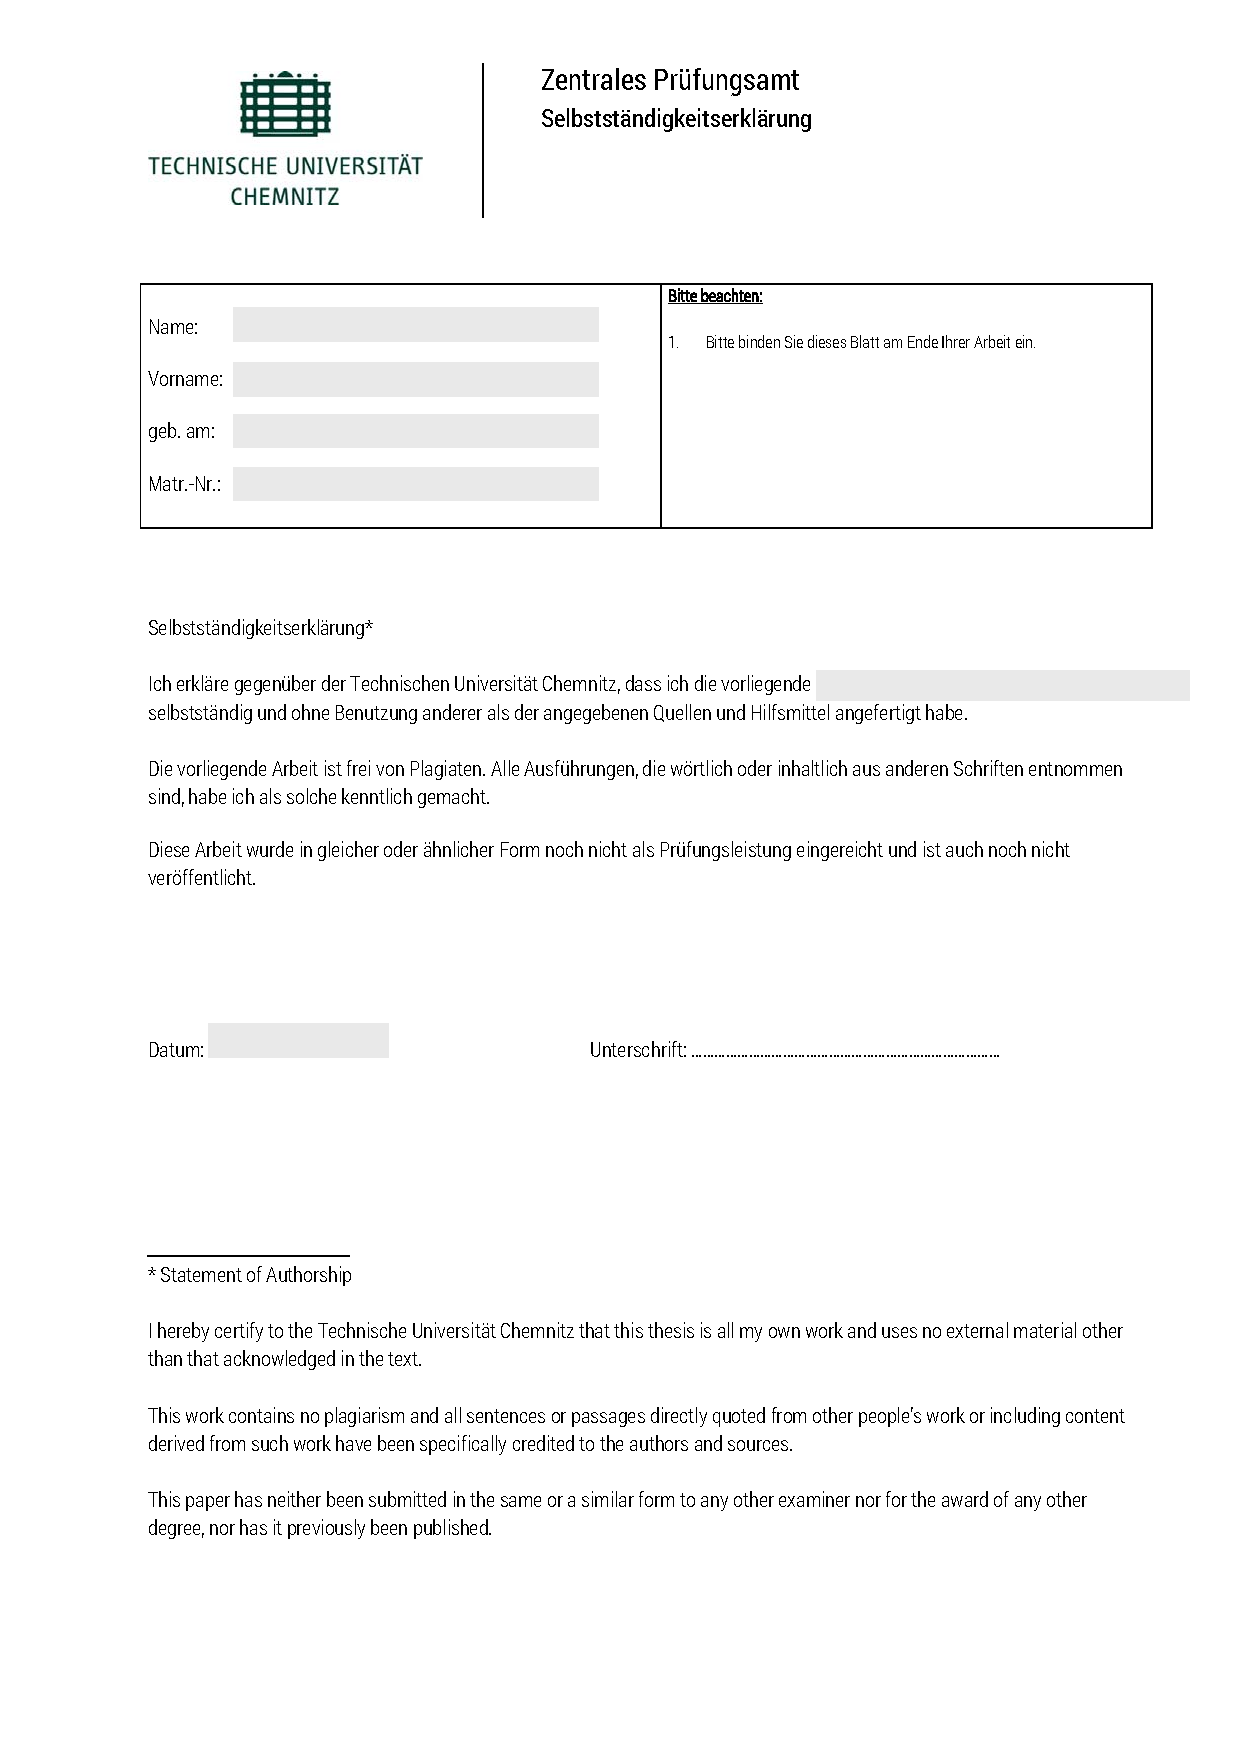
\includepdf[pages=-]{files/abschlussarbeit_selbststaendigkeitserklaerung.pdf} % you should replace this pdf with a filled-out version of your own % TODO: upload and replace the PDF with a filled-out version!
\end{document}
